
\newcommand{\packagename}[2]{\texttt{PACKAGENAME packagename}---keyword and name of this instance of the {#1} Package. \texttt{packagename} must be provided as a string, with no more than 16 characters. If not provided, then this {#1} Package instance will be given the name {#2}\_ibcnum, where ibcnum is the sequential {#1} Package number as determined by the order in the GWF Name File.}

\newcommand{\auxname}[1]{\texttt{AUXILIARY auxname [auxname2 [auxname3] ...]}---defines a list of one or more auxiliary variables, with the names \texttt{auxname}, \texttt{auxname2}, and so forth.  There is no limit on the number of auxiliary variables that can be provided on this line; however, lists of information provided in subsequent blocks must have a column of data for each auxiliary variable defined here.   Comments cannot be provided anywhere on this line as they will be interpreted as auxiliary variable names.  Auxiliary variables may not be used by the {#1} model, but they will be available for use by other parts of the program.  The ``AUX'' keyword can be used as a substitute for ``AUXILIARY''. The program will terminate with an error if auxiliary variables are specified on more than one line in the options block.}  

\newcommand{\auxmultname}[1]{\texttt{AUXMULTNAME auxnamemult}---name of auxiliary variable to be used as multiplier of {#1}.}

\newcommand{\boundnames}[1]{\texttt{BOUNDNAMES}---keyword to indicate that boundary names may be provided with the list of {#1} cells.}

\newcommand{\boundnamesnotlayered}[1]{\texttt{BOUNDNAMES}---keyword to indicate that boundary names may be provided with the list of {#1} cells. Incompatible with the READASARRAYS option.}

%\newcommand{\layered}{\texttt{LAYERED}---keyword to indicate that input will be read as arrays. Invalid for an unstructured grid (DISU).}

\newcommand{\printinput}[1]{\texttt{PRINT\_INPUT}---keyword to indicate that the list of {#1} information will be written to the listing file immediately after it is read.}

\newcommand{\printflows}[1]{\texttt{PRINT\_FLOWS}---keyword to indicate that the list of {#1} flow rates will be printed to the listing file for every stress period in which ``BUDGET PRINT'' is specified in Output Control.  If there is no Output Control option and \texttt{PRINT\_FLOWS} is specified, then flow rates are printed for the last time step of each stress period.}

\newcommand{\saveflows}[1]{\texttt{SAVE\_FLOWS}---keyword to indicate that {#1} flow terms will be written to the file specified with ``BUDGET SAVE FILE'' in Output Control.}

\newcommand{\timeseries}[0]{\texttt{TIMESERIESFILE time-series-filename}---defines a time-series file defining time series that can be used to assign time-varying values. See the ``Time-Variable Input'' section for instructions on using the time-series capability.}

\newcommand{\timearrayseries}{\texttt{TIMEARRAYSERIESFILE time-array-series-filename}---defines a time-array-series file defining a time-array series that can be used to assign time-varying values. See the ``Time-Variable Input'' section for instructions on using the time-array series capability.}

\newcommand{\timearrayserieslayered}{\texttt{TIMEARRAYSERIESFILE time-array-series-filename}---name of a time-array-series file defining a time-array series that can be used to assign time-varying values when input is read in array form. See the ``Time-Variable Input'' section for instructions on using the time-array series capability. Valid only when the READASARRAYS option is used.}

\newcommand{\maxbound}[1]{\texttt{MAXBOUND maxbound}---keyword and integer value specifying the maximum number of {#1} cells that will be specified for use during any stress period.}

\newcommand{\iper}[1]{\texttt{BEGIN PERIOD iper}---keywords and integer value specifying the starting stress period number for which the following list of {#1} cells will apply.  The list of {#1} cells specified in this block will remain active with their specified head values until a new ``BEGIN PERIOD'' block is detected.}

\newcommand{\cellid}[0]{\texttt{cellid}---is the cell identifier, and depends on the type of grid that is used for the simulation.  For a structured grid that uses the DIS input file, \texttt{cellid} is the layer, row, and column.   For a grid that uses the DISV input file, \texttt{cellid} is the layer and cell2d number.  If the model uses the unstructured discretization (DISU) input file, then \texttt{cellid} is the node number for the cell.}

\newcommand{\xyzaux}[1]{\texttt{x,y,z}---represents the values of the auxiliary variables for each {#1}. The values of auxiliary variables must be present for each {#1}. The values must be specified in the order of the auxiliary variables specified in the OPTIONS block.  If the package supports time series and the Options block includes a TIMESERIESFILE entry (see the ``Time-Variable Input'' section), values can be obtained from a time series by entering the time-series name in place of a numeric value.}

\newcommand{\boundname}[1]{\texttt{boundname}---name of the {#1} cell.  \texttt{boundname} is an ASCII character variable that can contain as many as 40 characters.  If \texttt{boundname} contains spaces in it, then the entire name must be enclosed within single quotes.}

\newcommand{\newtonopt}[1]{\texttt{NEWTON}---keyword that activates the Newton-Raphson formulation for the {#1} Package.}

\newcommand{\obsopt}[1]{\texttt{OBS8 observation-input-filename}---keyword and name of input file to define observations for the {#1} package. See the ``Observation utility'' section for instructions for preparing observation input files. Table \ref{table:obstype} lists observation type(s) supported by the {#1} package.}

\newcommand{\mover}[1]{\texttt{MOVER}---keyword to indicate that this instance of the {#1} Package can be used with the Water Mover (MVR) Package.  When the \texttt{MOVER} option is specified, additional memory is allocated within the package to store the available, provided, and received water.}

\newcommand{\packageperioddescription}{All of the stress package information in the PERIOD block will continue to apply for subsequent stress periods until the end of the simulation, or until another PERIOD block is encountered.  When a new PERIOD block is encountered, all of the stresses from the previous block are replaced with the stresses in the new PERIOD block.  Note that this behavior is different from the advanced packages (MAW, SFR, LAK, and UZF).  To turn off all of the stresses for a stress period, a PERIOD block must be specified with no entries.  If a PERIOD block is not specified for the first stress period, then no stresses will be applied until the \texttt{iper} value of the first PERIOD block in the file.}

\newcommand{\gwepackageperioddescription}{All of the stress package information in the PERIOD block will continue to apply for subsequent stress periods until the end of the simulation, or until another PERIOD block is encountered.  When a new PERIOD block is encountered, all of the stresses from the previous block are replaced with the stresses in the new PERIOD block.  Note that this behavior is different from the advanced packages (MWE, SFE, LKE, and UZE).  To turn off all of the stresses for a stress period, a PERIOD block must be specified with no entries.  If a PERIOD block is not specified for the first stress period, then no stresses will be applied until the \texttt{iper} value of the first PERIOD block in the file.}

\newcommand{\packageperioddescriptionarray}[1]{All of the stress package information in the PERIOD block will continue to apply for subsequent stress periods until the end of the simulation, or until another PERIOD block is encountered.  When a new PERIOD block is encountered, the array-based input specified by the user will replace the arrays currently in memory.  If an array is not specified in the period block, then that array will retain its present values in memory.  With the array-based input, the user must specify a {#1} rate of zero in order to turn {#1} off for a stress period.  This behavior is different from list-based input in which an empty PERIOD block results in no stresses being applied.}

\newcommand{\advancedpackageperioddescription}[2]{All of the advanced stress package information in the PERIOD block will continue to apply for subsequent stress periods until the end of the simulation, or until another PERIOD block is encountered.  When a new PERIOD block is encountered only the {#2} specified in the new period block will be changed.  A {#1} not specified in the new period block will continue to behave according to its specification in the previous PERIOD block.  Note that this behavior is different from the simple stress packages (CHD, WEL, DRN, RIV, GHB, RCH and EVT), in which any stress not specified in a new PERIOD block will be removed.  To turn off all of the advanced stresses for a stress period, a PERIOD block must be specified with settings that deactivate the {#2}.  If a PERIOD block is not specified for the first stress period, then no stresses will be applied.}


%Introduction for input instructions
\SECTION{Introduction}
This document is a technical reference document that describes the motivation and implementation of functionality added to \mf since the initial release \citep{modflow6framework, modflow6gwf} and not documented in separate U.S. Geological Survey publications, for example \cite{modflow6xt3d}. Examples have been included for the \mf components summarized in table~\ref{table:mf6enhance}.

\begin{table}[!ht]
  \small
  \centering
  \caption{\mf enhancements} \tabularnewline 

  \begin{tabular}{z{3.50cm}
                  z{3.50cm}
                  z{3.50cm}
                  z{3.50cm}
                  }
    % header
    \hline
    \rowcolor{Gray}
    \multicolumn{1}{ z{3.50cm} }{\textbf{\mf enhancements}} & 
    \multicolumn{1}{ z{3.50cm} }{\textbf{Chapter}} & 
    \multicolumn{1}{ z{3.50cm} }{\textbf{Initial \mf version}} & 
    \multicolumn{1}{ z{3.50cm} }{\textbf{Latest update -- \mf version}} \\
    \hline

    Specific Discharge &  \ref{ch:spdis} & 6.0.2    &  6.1.0  \\
\rowcolor{Gray}
    DRN Package Discharge Scaling &  \ref{ch:drn} & 6.1.1    &  --   \\
    MAW Package Connection Flow Correction &  \ref{ch:maw-qcorr} & 6.1.1    &  --   \\
\rowcolor{Gray}
    STO Package Specific Storage Revision &  \ref{ch:sto-mod} & 6.1.3    &  --   \\
    TVK and TVS Capabilities for NPF & \ref{ch:tvk-tvs} & 6.3.0  &  -- \\
\rowcolor{Gray}
    Generalized Coupling of Numerical Models & \ref{ch:gencouple} & 6.3.0 & -- \\
    VSC Package & \ref{ch:vscpackage} & 6.4.0 & -- \\
\rowcolor{Gray}
    Revised Parameterization of Transport for Combined Mobile and Immobile Domain Simulations & \ref{ch:sorption} & 6.4.2 & -- \\
    Groundwater Energy (GWE) Model & \ref{ch:gwemodel} & 6.5.0 & -- \\
\rowcolor{Gray}
    Particle Tracking (PRT) Model & \ref{ch:prtmodel} & 6.5.0 & -- \\
    \hline
  \end{tabular}
  \label{table:mf6enhance}
\end{table}




%Instructions for running a simulation
\SECTION{Running a Simulation}
\input{running_simulation.tex}

%General form of input instructions
\SECTION{Form of Input Instructions}
\mf differs from its predecessors in the form of the input.  Whereas previous MODFLOW versions read numerical values, arrays, and lists in a highly structured form, \mf reads information in the form of blocks and keywords.  \mf also reads arrays and lists of information, but these arrays and lists are tagged with identifying block names or keywords.  \mf will terminate with an error if it detects an unrecognized block or keyword.

\subsection{Block and Keyword Input} 

Input to \mf is provided within blocks.  A block is a section of an ASCII input file that begins with a line that has ``BEGIN'' followed by the name of the block and ends with a line the begins with ``END'' followed by the name of the block.  \mf will terminate with an error if blocks do not begin and end with the same name, or if a ``BEGIN'' or ``END'' line is missing.  Information within a block differs depending on the part of \mf that reads the block.  In general, keywords are used within blocks to turn options on or specify the type of information that follows the keyword.  If an unrecognized keyword is encountered in a block, \mf will terminate with an error.

The keyword approach is adopted in \mf to improve readability of the \mf input files, enhance discovery of errors in input files, and improve support for backward compatibility by allowing the program to expand in functionality while allowing previously developed models to be run with newer versions of the program.

Within these user instructions, keywords are shown in capital letters to differentiate them from other input that is provided by the user.  For example, ``BEGIN'' and ``END'' are recognized by \mf, and so they are capitalized.  Also, line indentation is used within these user instructions to help with readability of the blocks.  Typically, lines within a block are indented two spaces to accentuate that the lines are part of the block.  This indentation is not enforced by the program, but users are encouraged to use it within their own input files to improve readability.

Unless stated otherwise in this user guide, information contained within a block can be listed in any order.  If the same keyword is provided more than once, then the program will use the last information provided by that keyword.

Comment lines and blanks lines are also allowed within most blocks and within most input files.  Valid comment characters include ``\#'' ``!'', and ``//''.  Comments can also be placed at the end of some input lines, after the required information.  Comments are not allowed at the end of some lines if the program is required to read an arbitrary number of non-keyword items.  Comments included at the end of the line must be separated from the rest of the line by at least one space.

Unless otherwise noted in the input instructions, multiple blocks of the same name cannot be specified in a single input file.  The block order within the input file must follow the order presented in the input instructions.  Each input file typically begins with an OPTIONS block, which is generally not required, followed by one or more data blocks.

The following is an example of how the input instructions for a block are presented in this document.  
\begin{lstlisting}[style=blockdefinition]
BEGIN OPTIONS
  [AUXILIARY <auxiliary(naux)>]
  [PRINT_INPUT]
  [MAXIMUM_ITERATION <maxsfrit>]
END OPTIONS
\end{lstlisting}
This example shows the items that may be specified with this OPTIONS block.  Optional items are enclosed between ``['' and ``]'' symbols.  The ``\texttt{<}'' and ``\texttt{>}'' symbols indicate a variable that must be provided by the user.  In this case, \texttt{auxiliary} is an array of size \texttt{naux}.  Because there are bracket symbols around the entire item, the user it not required to specify anything for this item.  Likewise, the user may or may not invoke the ``\texttt{PRINT\_INPUT}'' option.  Lastly, the user can specify ``\texttt{MAXIMUM\_ITERATION}'' followed by a numeric value for ``\texttt{maxsfrit}''.  If the user does not specify an optional item, then a default condition will apply.  Behavior of the default condition is described in the input instructions for that item.

\vspace{6pt}\noindent A valid user input block for OPTIONS might be:

\begin{lstlisting}[style=inputfile]
#This is my options block
BEGIN OPTIONS
  AUXILIARY temperature salinity
  MAXIMUM_ITERATION 10
END OPTIONS
\end{lstlisting}

\noindent The following is another valid user input block for OPTIONS:

\begin{lstlisting}[style=inputfile]
#This is an alternative options block
BEGIN OPTIONS
  # Assign two auxiliary variables
  AUXILIARY temperature salinity
  # Specify the maximum iteration
  MAXIMUM_ITERATION 10
  #specify the print input option
  PRINT_INPUT
END OPTIONS
#done with the options block
\end{lstlisting}

\subsection{Specification of Block Information in OPEN/CLOSE File} 
For most blocks, information can be read from a separate text file.  In this case, all of the information for the block must reside in the text file.  The file name is specified using the OPEN/CLOSE keyword as the first and only entry in the block as follows:

\begin{lstlisting}[style=inputfile]
#This is an alternative options block
BEGIN OPTIONS
  OPEN/CLOSE myoptblock.txt
END OPTIONS
\end{lstlisting}

\noindent When MODFLOW encounters the OPEN/CLOSE keyword, the program opens the specified file on unit 99 and continues processing the information in the file as if it were within the block itself.  When the program reaches the end of the file, the file is closed, and the program returns to reading the original package file.  The next line after the OPEN/CLOSE line must end the block.

Some blocks do not support the OPEN/CLOSE capability.  A list of all of the blocks, organized by component and input file type, are listed in a table in appendix A.  This table also indicates the blocks that do not support the OPEN/CLOSE capability.

\subsection{Text Color}

Note that text color in the input instructions is indicative of special features or behaviors associated with the variables printed in that color.  Specifically, the {\color{blue} text color of blue} is reserved to indicate a variable that may be represented with a time series.  The {\color{red} text color of red} is reserved for keywords or variables that are supported only in the extended build of \mf.  The extended build is covered in its own section in this document.


\subsection{File Name Input}
Some blocks may require that a file name be entered.  Although spaces within a file name are not generally recommended, they can be specified if the entire file name is enclosed within single quotes, which means that the file name itself cannot have a single quote within it.  On Windows computers, file names are not case sensitive, and thus, ``model.dis'' can be referenced within the input files as ``MODEL.DIS''.  On some other operating systems, however, file names are case sensitive and the case used in the input instructions must exactly reflect the case used to name the file.

\subsection{Lengths of Character Variables}
Character variables, which are used to store names of models, packages, observations and other objects, are limited in the number of characters that can be used. Table \ref{table:characterlength} lists the limit used for each type of character variable.

\FloatBarrier
\begin{table}[H]
\caption{Character variable maximum sizes}
\small
\begin{center}
\begin{tabular*}{\columnwidth}{l l l}
\hline
\hline
\textbf{Size limit name} & \textbf{Size} & \textbf{Variable(s) affected} \\
\hline
LENAUXNAME & 16 & Auxiliary variable names \\
LENBOUNDNAME & 40 & Boundary names \\
LENMODELNAME & 16 & Model names \\
LENOBSNAME & 40 & Observation names \\
LENPACKAGENAME & 16 & Package names \\
LENSOLUTIONNAME & 16 & Solution names \\
LENTIMESERIESNAME & 40 & Time-series and time-array-series names \\
\hline
\end{tabular*}
\label{table:characterlength}
\end{center}
\normalsize
\end{table}

\FloatBarrier

\subsection{Integer and Floating Point Variables}
\mf uses integer and floating point variables throughout the program.  The sizes of these variables are defined in a single module within the program.  Information about the precision, range, and size of integers and floating point real variables is written to the top of the simulation list file: 

{\small
\begin{lstlisting}[style=modeloutput]
MODFLOW was compiled using uniform precision.

Real Variables
  KIND: 8
  TINY (smallest non-zero value):    2.225074-308
  HUGE (largest value):    1.797693+308
  PRECISION: 15
  SIZE IN BITS: 64

Integer Variables
  KIND: 4
  HUGE (largest value): 2147483647
  SIZE IN BITS: 32

Long Integer Variables
  KIND: 8
  HUGE (largest value): 9223372036854775807
  SIZE IN BITS: 64

Logical Variables
  KIND: 4
  SIZE IN BITS: 32
\end{lstlisting}
}

This information indicates that real variables have about 15 digits of precision.  The smallest positive non-zero value that can be stored is 2.2e-308.  The largest value that can be stored is 1.8e+308.  If the user enters a value in an input file that cannot be stored, such as 1.9335e-310 for example, then the program can produce unexpected results.  This does not affect an exact value of zero, which can be stored accurately.  Integer variables also have a maximum and minimum value, which is about 2 billion.  Values larger and smaller than this cannot be stored.  These numbers are rarely exceeded for most practical problems, but as the size of models (number of nodes) increase into the billions, then the program may need to be recompiled using a larger size for integer variables. Long integers are used to calculate the amount of memory allocated in the memory manager:

{\small
\begin{lstlisting}[style=modeloutput]
 MEMORY MANAGER TOTAL STORAGE BY DATA TYPE, IN MEGABYTES
 -------------------------------
                    ALLOCATED   
 DATA TYPE           MEMORY     
 -------------------------------
 Character        1.53300000E-03
 Logical          4.40000000E-05
 Integer          100.03799     
 Real             223.43994     
 -------------------------------
 Total            323.47951     
 -------------------------------
\end{lstlisting}
}

Currently, standard precision 4 byte logical variables are used throughout the program.

\subsection{Array Input (READARRAY)}
Some \mf Model packages require arrays of information to be provided by the user.  This information is read using a generic READARRAY capability in \mf.  Within this user guide, variables that are read with READARRAY are marked accordingly, as shown in example input instructions for a DATA block.  

\begin{lstlisting}[style=blockdefinition]
BEGIN DATA
  ARRAY1
    <array1(nval)> -- READARRAY
END DATA
\end{lstlisting}

\noindent In this example, the uppercase ARRAY1 is a text string that is recognized by the program.  While reading through the DATA block, the program would recognize ARRAY1, and would then use READARRAY to fill \texttt{array1} with \texttt{nval} values.

\subsubsection{READARRAY Control Line}

READARRAY works similar to the array readers in previous MODFLOW versions.  It begins by reading a control line.  The control line has one of three forms shown below, and is limited to a length of 999 characters.

\begin{lstlisting}[style=blockdefinition]
1. CONSTANT <constant> 
\end{lstlisting}
With CONSTANT, all values in the array are set equal to \texttt{constant}. 

\begin{lstlisting}[style=blockdefinition]
2. INTERNAL [FACTOR <factor>] [IPRN <iprn>] 
\end{lstlisting}
With INTERNAL, the individual array elements will be read from the same file that contains the control line. 

\begin{lstlisting}[style=blockdefinition]
3. OPEN/CLOSE <fname> [FACTOR <factor>] [(BINARY)] [IPRN <iprn>]
\end{lstlisting}
With OPEN/CLOSE, the array will be read from the file whose name is specified by \texttt{fname}. This file will be opened just prior to reading the array and closed immediately after the array is read. A file that is read using this control line can contain only a single array. 

\subsubsection{READARRAY Variable Descriptions}

\begin{description}

\item \texttt{<constant>}---is a real number constant for real arrays and an integer constant for integer arrays. The \texttt{constant} value is assigned to the entire array. 

\item \texttt{FACTOR <factor>}---are a keyword and a real number factor for real arrays and an integer factor for integer arrays. The individual elements of the array are multiplied by \texttt{factor} after they are read. If \texttt{factor} is specified as 0, then it is changed to 1.

\item \texttt{(BINARY)}---is an option that indicates the OPEN/CLOSE file contains array data in binary (unformatted) form. A binary file that can be read by MODFLOW may be created in only two ways. The first way is to use MODFLOW to create the file by saving heads in a binary file. This is commonly done when the user desires to use computed heads from one simulation as initial heads for a subsequent simulation. The other way to create a binary file is to write a special program that generates a binary file.  ``(BINARY)'' can be specified only when the control line is OPEN/CLOSE.

\item \texttt{IPRN <iprn>}---are a keyword and a flag that indicates whether the array being read should be written to the Listing File after the array has been read and a code for indicating the format that should be used when the array is written. The format codes are the same as for MODFLOW-2005. IPRN is set to zero when the specified value exceeds those defined. If IPRN is less than zero or if the keyword and flag are omitted, the array will not be printed.  This IPRN capability is not functional for all data sets, and will eventually become unsupported for all packages.  For some packages that have transitioned to the new input data processor, the EXPORT\_ARRAY\_ASCII option can be specified in the package OPTIONS block.  When this option is active, input arrays will be written to external text files.

\end{description}

\begin{longtable}{p{2cm} p{2cm} p{2cm} p{2cm}}
\caption{IPRN Code and corresponding print formats for array readers.  These print codes determine how the user-provided array is written to the list file} 
\tabularnewline
\hline
\hline
\textbf{IPRN} & \textbf{Real} & \textbf{Integer} \\
\hline
\endhead
\hline
\endfoot
0 & 10G11.4 & 10I11 \\
1 & 11G10.3 & 60I1 \\
2 & 9G13.6 & 40I2 \\
3 & 15F7.1 & 30I3 \\
4 & 15F7.2 & 25I4 \\
5 & 15F7.3 & 20I5 \\
6 & 15F7.4 & 10I11 \\
7 & 20F5.0 & 25I2 \\
8 & 20F5.1 & 15I4 \\
9 & 20F5.2 & 10I6 \\
10 & 20F5.3 &  \\
11 & 20F5.4 &  \\
12 & 10G11.4 & \\
13 & 10F6.0 &  \\
14 & 10F6.1 &  \\
15 & 10F6.2 &  \\
16 & 10F6.3 &  \\
17 & 10F6.4 &  \\
18 & 10F6.5 &  \\
19 & 5G12.5 &  \\
20 & 6G11.4 &  \\
21 & 7G9.2 &  \\
%\label{table:ndim}
\end{longtable}


\subsubsection{READARRAY Examples}

The following examples use free-format control lines for reading an array. The example array is a real array consisting of 4 rows with 7 columns per row: 

\begin{lstlisting}[style=inputfile]
CONSTANT 5.7      This sets an entire array to the value "5.7". 
INTERNAL FACTOR 1.0 IPRN 3            This reads the array values from the 
 1.2 3.7 9.3 4.2 2.2 9.9 1.0      file that contains the control line. 
 3.3 4.9 7.3 7.5 8.2 8.7 6.6      Thus, the values immediately follow the 
 4.5 5.7 2.2 1.1 1.7 6.7 6.9      control line. 
 7.4 3.5 7.8 8.5 7.4 6.8 8.8 
OPEN/CLOSE inp.txt FACTOR 1.0 IPRN 3    Read array from formatted file "inp.dat". 
OPEN/CLOSE inp.bin FACTOR 1.0 (BINARY) IPRN 3     Read array from binary file "inp.bin". 
OPEN/CLOSE test.dat FACTOR 1.0 IPRN 3     Read array from file "test.dat". 
\end{lstlisting}


Some arrays define information that is required for the entire model grid, or part of a model grid.  This type of information is provided in a special type of data block called a ``GRIDDATA'' block.  For example, hydraulic conductivity is required for every cell in the model grid.  Hydraulic conductivity is read from a ``GRIDDATA'' block in the \mf GWF NPF Package input file.  For GRIDDATA arrays with one value for every cell in the model grid, the arrays can optionally be read in a LAYERED format, in which an array is provided for each layer of the grid.  Alternatively, the array can be read for the entire model grid.  As an example, consider the GRIDDATA block for the \mf GWF or GWT IC Package shown below:

\lstinputlisting[style=blockdefinition]{./mf6ivar/tex/gwf-ic-griddata.dat}

Here, the initial heads for the model are provided in the \texttt{strt} array.  If the optional LAYERED keyword is present, then a separate array is provided for each layer.  If the LAYERED keyword is not present, then the entire starting head array is read at once.  The LAYERED keyword may be useful to discretization packages of type DIS and DISV, which support the concept of layers.  Models defined with the DISU Package are not layered.

Note that the \mf Extended build also supports an optional NETCDF keyword.  This keyword is not compatible with the LAYERED keyword and is a valid option only if a model NetCDF input file is configured.  This type of workflow is covered in the section which describes Extended \mf.

For a structured DIS model, the READARRAY utility is used to read arrays that are dimensioned to the full size of the grid (of size \texttt{nlay*nrow*ncol}). This utility first reads an array name, which associates the input to be read with the desired array.  For these arrays, an optional keyword ``LAYERED'' can be located next to the array name.  If ``LAYERED'' is detected, then a control line is provided for each layer and the array is filled with values for each model layer.  If the ``LAYERED'' keyword is absent, then a single control line is used and the entire array is filled at once.

For example, the following block shows one way the \mf GWF model starting head array (STRT) could be specified for a model with 4 layers.  Following the array name and the ``LAYERED'' keyword are four control lines, one for each layer.

\begin{lstlisting}[style=inputfile]
  STRT LAYERED
     CONSTANT 10.0  #layer 1
     CONSTANT 10.0  #layer 2
     CONSTANT 10.0  #layer 3
     CONSTANT 10.0  #layer 4
\end{lstlisting}

In this next example, the ``LAYERED'' keyword is absent.  In this case, the control line applies to the entire \texttt{strt} array.  One control line is required, and a constant value of 10.0 will be assigned to STRT for all cells in the model grid.

\begin{lstlisting}[style=inputfile]
  STRT
     CONSTANT 10.0  #applies to all cells in the grid
\end{lstlisting}

In the next example, the ``LAYERED'' keyword is present and binary files are used for each layer. A control line with the ``BINARY'' keyword is required for each layer.

\begin{lstlisting}[style=inputfile]
  STRT LAYERED
     OPEN/CLOSE strt.layer1.bin (BINARY)  #layer1
     OPEN/CLOSE strt.layer2.bin (BINARY)  #layer2
     OPEN/CLOSE strt.layer3.bin (BINARY)  #layer3
     OPEN/CLOSE strt.layer4.bin (BINARY)  #layer4
\end{lstlisting}

In the next example, the ``LAYERED'' keyword is absent. In this case, a single control line with the ``BINARY'' keyword is required and the binary file will include the entire data array.

\begin{lstlisting}[style=inputfile]
  STRT
     OPEN/CLOSE strt.bin (BINARY)  #layers1-4
\end{lstlisting}

A consequence of the way binary input files have been implemented in \mf, simulated dependent variable binary output (for example, head and concentration) cannot be used as binary array input for a model. Instead, simulated dependent variable binary output must be processed and split into separate binary files for each layer or combined into a single array equal to the size of the grid (for DIS grids this would be an array equal to NCOL * NROW * NLAY).

\subsubsection{Description of Binary Array Input Files}
All floating point variables are written to the binary input files as DOUBLE PRECISION Fortran variables. Integer variables are written to the input files as Fortran integer variables. Some variables are character strings and are indicated as so in the following descriptions. Binary array data are written using the following two records:

\vspace{5mm}
\noindent Record 1: \texttt{KSTP,KPER,PERTIM,TOTIM,TEXT,M1,M2,M3} \\
\noindent Record 2: \texttt{DATA} \\

\vspace{5mm}
\noindent where

\begin{description} \itemsep0pt \parskip0pt \parsep0pt
\item \texttt{KSTP} is the time step number;
\item \texttt{KPER} is the stress period number;
\item \texttt{PERTIM} is the time value for the current stress period; 
\item \texttt{TOTIM} is the total simulation time;
\item \texttt{TEXT} is a character string (character*16);
\item \texttt{M1} is the length of the data in the fastest varying direction;
\item \texttt{M2} is the length of the data in the second fastest varying direction;
\item \texttt{M3} can be any value but is typically 1 or the layer number for the data; and
\item \texttt{DATA} is the array data of size (M1*M2).
\end{description}
 
\noindent The values specified for \texttt{M1}, \texttt{M2}, and \texttt{M3} in Record 1 are dependent on the grid type and if the ``LAYERED'' keyword is present on the READARRAY control line.  For binary array data, \texttt{KSTP}, \texttt{KPER}, \texttt{PERTIM}, \texttt{TOTIM}, and \texttt{TEXT} can be set to any value. Binary array input file specifications for each discretization type are given below.

\paragraph{DIS Grids}
For DIS grids,  \texttt{M1=NCOL}, \texttt{M2=NROW}, and \texttt{M3=ILAY} when the ``LAYERED'' keyword is present on the READARRAY control line. For this case, record 1 and 2 should be written as:

\vspace{5mm}
\noindent Record 1: \texttt{KSTP,KPER,PERTIM,TOTIM,TEXT,M1,M2,M3} \\
\noindent Record 2: \texttt{((DATA(J,I,ILAY),J=1,NCOL),I=1,NROW)} \\

\vspace{5mm}
\noindent where

\begin{description} \itemsep0pt \parskip0pt \parsep0pt
\item \texttt{NCOL} is the number of columns;
\item \texttt{NROW} is the number of rows; and
\item \texttt{ILAY} is the layer number.
\end{description}

\noindent For DIS grids, \texttt{M1=NCOL*NROW*NLAY}, \texttt{M2=1}, and \texttt{M3=1} when the ``LAYERED'' keyword is absent on the READARRAY control line. For this case, record 1 and 2 should be written as:

\vspace{5mm}
\noindent Record 1: \texttt{KSTP,KPER,PERTIM,TOTIM,TEXT,M1,M2,M3} \\
\noindent Record 2: \texttt{(((DATA(J,I,K),J=1,NCOL),I=1,NROW),K=1,NLAY)} \\

\vspace{5mm}
\noindent where

\begin{description} \itemsep0pt \parskip0pt \parsep0pt
\item \texttt{NLAY} is the number of layers.
\end{description}

\paragraph{DISV Grids}
For DISV grids, \texttt{M1=NCPL}, \texttt{M2=1}, and \texttt{M3=ILAY} when the ``LAYERED'' keyword is present on the READARRAY control line. For this case, record 1 and 2 should be written as:

\vspace{5mm}
\noindent Record 1: \texttt{KSTP,KPER,PERTIM,TOTIM,TEXT,M1,M2,M3} \\
\noindent Record 2: \texttt{(DATA(J,ILAY),J=1,NCPL)} \\

\vspace{5mm}
\noindent where

\begin{description} \itemsep0pt \parskip0pt \parsep0pt
\item \texttt{NCPL} is the number of cells per layer.
\end{description}

\noindent For DISV grids, \texttt{M1=NCPL*NLAY}, \texttt{M2=1}, and \texttt{M3=1} when the ``LAYERED'' keyword is absent on the READARRAY control line. For this case, record 1 and 2 should be written as:

\vspace{5mm}
\noindent Record 1: \texttt{KSTP,KPER,PERTIM,TOTIM,TEXT,M1,M2,M3} \\
\noindent Record 2: \texttt{((DATA(J,K),J=1,NCPL),K=1,NLAY)} \\


\paragraph{DISU Grids}
For DISU grids, \texttt{M1=NODES}, \texttt{M2=1}, \texttt{M3=1}. For this case, record 1 and 2 should be written as:


\vspace{5mm}
\noindent Record 1: \texttt{KSTP,KPER,PERTIM,TOTIM,TEXT,M1,M2,M3} \\
\noindent Record 2: \texttt{(DATA(N),N=1,NODES)} \\

\vspace{5mm}
\noindent where

\begin{description} \itemsep0pt \parskip0pt \parsep0pt
\item \texttt{NODES} is the number cells in the model grid.
\end{description}

\subsection{List Input}
Some items consist of several variables, such as layer, row, column, stage, and conductance, for example.  List input refers to a block of data with a separate item on each line.  For some common list types, the first set of variables is a cell identifier (denoted as \texttt{cellid} in this guide), such as layer, row, and column. With lists, the input data for each item must start on a new line. All variables for an item are assumed to be contained in a single line.  Each input variable has a data type, which can be Double Precision, Integer, or Character. Integers are whole numbers and must not include a decimal point or exponent. Double Precision numbers can include a decimal point and an exponent. If no decimal point is included in the entered value, then the decimal point is assumed to be at the right side of the value. Any printable character is allowed for character variables. 

Variables starting with the letters I-N are most commonly integers; however, in some instances, a character string may start with the letters I-N. Variables starting with the letters A-H and O-Z are primarily double precision numbers; however, these variable names may also be used for character data.  In \mf all variables are explicitly declared within the source code, as opposed to the implicit type declaration in previous MODFLOW versions.  This explicit declaration means that the variable type can be easily determined from the source code.

Free formatting is used throughout the input instructions.  With free format, values are not required to occupy a fixed number of columns in a line. Each value can occupy one or more columns as required to represent the value; however, the values must still be included in the prescribed order. One or more spaces, or a single comma optionally combined with spaces, must separate adjacent values. Also, a numeric value of zero must be explicitly represented with 0 and not by one or more spaces when free format is used, because detecting the difference between a space that represents 0 and a space that represents a value separator is not possible. Free format is similar to Fortran's list directed input.

Two capabilities included in Fortran's list-directed input are not included in the free-format input implemented in \mf. Null values in which input values are left unchanged from their previous values are not allowed. In general, MODFLOW's input values are not defined prior to their input.  A ``/'' cannot be used to terminate an input line without including values for all the variables; data values for all required input variables must be explicitly specified on an input line.  For character data, MODFLOW's free format implementation is less stringent than the list-directed input of Fortran. Fortran requires character data to be delineated by apostrophes. MODFLOW does not require apostrophes unless a blank or a comma is part of a character variable.

As an example of a list, consider the PERIOD block for the GHB Package.  The input format is  shown below:

\lstinputlisting[style=blockdefinition]{./mf6ivar/tex/gwf-ghb-period.dat}

Each line represents a separate item, which consists of variables.  In this case, the first variable of the item, \texttt{cellid} is an array of size \texttt{ncelldim}.  The next two variables of the item are \texttt{bhead} and \texttt{cond}.  Lastly, the item has two optional variables, \texttt{aux} and \texttt{boundname}.  Three of the variables shown in the list are colored in blue.  Variables that are colored in blue mean that they can be represented with a time series.  The time series capability is described in the section on Time-Variable Input in this document.  

The following is simple example of a PERIOD block for the GHB Package, which shows how a list is entered by the user.

\begin{lstlisting}[style=inputfile]
BEGIN PERIOD 1
#      lay       row       col     stage      cond
         1        13         1     988.0     0.038
         1        14         9    1045.0     0.038
END PERIOD
\end{lstlisting}

As described earlier in the section on ``Block and Keyword Input,'' block information can be read from a separate text file.  To activate reading a list from separate text file, the first and only entry in the block must be a control line of the following form:  

\begin{lstlisting}[style=blockdefinition]
  OPEN/CLOSE <fname>
\end{lstlisting}

\noindent where \texttt{fname} is the name of the file containing the list.  Lists for the stress packages (CHD, WEL, DRN, RIV, GHB, RCH, and EVT) have an additional BINARY option.  The BINARY  option is not supported for the advanced stress packages (LAK, MAW, SFR, UZF, LKT, MWT, SFT, UZT).  The BINARY options is specified as follows:

\begin{lstlisting}[style=blockdefinition]
  OPEN/CLOSE <fname> [(BINARY)]
\end{lstlisting}

If the (BINARY) keyword is found on the control line, then the file is opened as an unformatted file on unit 99, and the list is read.  There are a number of requirements for using the (BINARY) option for lists.  All stress package lists begin with integer values for the \texttt{cellid} (layer, row, and column, for example).  These values must be represented as integer numbers in the unformatted file.  Also, all auxiliary data must be included in the binary file; auxiliary data must be represented as double precision numbers.  Lastly, the (BINARY) option does not support entry of \texttt{boundname}, and so the BOUNDNAMES option should not be activated in the OPTIONS block for the package.  
\subsubsection{Description of Binary List Input Files}
All floating point variables are written to the binary input files as DOUBLE PRECISION Fortran variables. Integer variables are written to the input files as Fortran integer variables. Auxiliary variables can be included in binary list input files but as indicated previously binary list input files can not be used for packages that include BOUNDNAMES keyword in the OPTIONS block. The format of binary list data are described below.

\vspace{5mm}
\noindent Record 1: \texttt{(CELLID(N),(RLIST(I,N),I=1,NDAT)(AUXVAR(I,N),I=1, NAUX), N=1,NLIST)}\\

\noindent where

\begin{description} \itemsep0pt \parskip0pt \parsep0pt
\item \texttt{CELLID} is the cell identifier, and depends on the type of grid that is used for the simulation.;
\item \texttt{RLIST} is a double precision two-dimensional array of size (NDAT,NLIST) containing the stress package PERIOD data;
\item \texttt{NDAT} is the number of columns in RLIST, which is the number of columns of real data in the stress package PERIOD data;
\item \texttt{AUXVAR} is a double precision two-dimensional array of size (NAUX,NLIST)  containing the auxiliary data for the stress package PERIOD data;
\item \texttt{NAUX} is the number of columns in AUXVAR, which is the number of columns of real auxiliary data the in stress package PERIOD data;
\item \texttt{NLIST} is the size of the list;
\end{description}

\noindent For a structured grid that uses the DIS input file, CELLID is the layer, row, and column. For a grid that uses the DISV input file, CELLID is the layer and CELL2D number. If the model uses the unstructured discretization (DISU) input file, CELLID is the node number for the cell. \texttt{NLIST} must be less than or equal to \texttt{MAXBOUND} for a stress package. \texttt{NAUX} is determined by the number of \texttt{AUXILIARY} variable names define in the OPTIONS block for the stress package.


%Processing of program input
\SECTION{Processing of Program Input}
An effort is underway to process program input early in program runtime, before the simulation is created, in a general way that is not dependent on any given component.  This capability is called the \mf Input Data Processor (IDP).  Components that have been updated to use IDP no longer directly read or process file inputs but instead access input data from internally managed memory locations. 

\subsection{Supported Components}

A specific set of \mf components has been updated in the current version to use the IDP routines, as shown in Table~\ref{table:idmsupported}.  Two integration steps have been taken for each file type listed in the table.  First, IDP has been updated to support the reading and loading of variable input data for the component.  File types listed in the table, each previously read and processed by the component, are now processed by IDP.  Second, the component itself has been refactored to retrieve input from managed memory locations in a predictable way.  Components and associated file types shown in table~\ref{table:idmsupported} are described in more detail in later sections of this document.

\begin{table}[H]
\caption{Components and subcomponents that are read using Input Data Processor (IDP) routines}
\small
\begin{center}
%\begin{tabular*}{\columnwidth}{l l}
\begin{longtable}{p{6cm} p{4cm}}
\hline
\hline
\textbf{Component / Subcomponent} & \textbf{File Type} \\
\hline
SIM/NAM & mfsim.nam \\
SIM/TDIS & TDIS6 \\
\hline
GWF/NAM & GWF name file \\
GWF/CHD & CHD6 \\
GWF/DIS & DIS6 \\
GWF/DISU & DISU6 \\
GWF/DISV & DISV6 \\
GWF/DRN & DRN6 \\
GWF/EVT & EVT6 \\
GWF/EVTA & EVT6 \\
GWF/GHB & GHB6 \\
GWF/IC & IC6 \\
GWF/NPF & NPF6 \\
GWF/RCH & RCH6 \\
GWF/RCHA & RCH6 \\
GWF/RIV & RIV6 \\
GWF/WEL & WEL6 \\
\hline
GWT/NAM & GWT name file \\
GWT/CNC & CNC6 \\
GWT/DIS & DIS6 \\
GWT/DISU & DISU6 \\
GWT/DISV & DISV6 \\
GWT/DSP & DSP6 \\
GWT/IC & IC6 \\
\hline
GWE/NAM & GWE name file \\
GWE/CND & CND6 \\
GWE/CTP & CTP6 \\
GWE/DIS & DIS6 \\ 
GWE/DISU & DISU6 \\
GWE/DISV & DISV6 \\
GWE/IC & IC6 \\
\hline
PRT/NAM & PRT name file \\
PRT/DIS & DIS6 \\ 
PRT/DISV & DISV6 \\
PRT/MIP & MIP \\
\hline
EXG/GWFGWF & GWF6-GWF6 \\
EXG/GWFGWT & GWF6-GWT6 \\
EXG/GWTGWT & GWT6-GWT6 \\
EXG/GWFGWE & GWF6-GWE6 \\
EXG/GWEGWE & GWE6-GWE6 \\
EXG/GWFPRT & GWF6-PRT6 \\
\hline
\end{longtable}
\label{table:idmsupported}
\end{center}
\normalsize
\end{table}

\subsection{Scope of Change}

The Input Data Processor introduces transparent changes that are beyond the scope of this document.  Input logging differences, however, are readily apparent when comparing to earlier versions of \mf.  These differences are primarily related to timing as input files processed by IDP are read before the simulation has been created.  Logging appears in the simulation log (mfsim.lst) in part because simulation models and their associated listing files do not exist at the time when input is read.  In addition, input logging reflects only what was read and loaded to memory as further processing and use is deferred to the simulation components that the input is intended for.  Summaries of memory managed variables, including input data variables loaded by IDP, are possible to view in the simulation listing files with a Simulation Name File option described later. 

\subsection{Example of Logging}

Below is an example of simulation logging (to the mfsim.lst output file) for two model package input files read and loaded by IDP routines.  The first logging block results from processing a DIS6 input file and the second logging block results from processing an NPF6 input file.  Variable names in the blocks are described in later sections of this document.

\small
\begin{lstlisting}[style=modeloutput]

 Loading input for GWF-NO-VSC-SFR01/DIS
 # File generated by Flopy version 3.3.7 on 05/31/2023 at 12:56:15.
   String detected: LENGTH_UNITS = M
   Integer detected: NLAY = 1
   Integer detected: NROW = 60
   Integer detected: NCOL = 200
   Double precision 1D constant array detected: DELR = 50.000000000000000
   Double precision 1D constant array detected: DELC = 50.000000000000000
   Double precision 2D array detected: TOP ranges from 230.07503124999999 to 303.32871875000001
   Double precision 3D constant array detected: BOTM = 0.0000000000000000
 Loading input complete...

 Loading input for GWF-NO-VSC-SFR01/NPF
 # File generated by Flopy version 3.3.7 on 05/31/2023 at 12:56:15.
   Keyword detected: SAVE_SPECIFIC_DISCHARGE
   Integer 1D constant array detected: ICELLTYPE = 1
   Double precision 1D constant array detected: K = 1.0000000000000000
 Loading input complete...
\end{lstlisting}


%Simulation name file
\newpage
\SECTION{Simulation Name File}
The simulation name file contains information about simulation options, simulation timing, models that are present in the simulation, how models exchange information, and how models are solved.

The present version of \mf uses the concept of a solution group.  For most simulations, a solution group will contain one solution and one model within that solution.  The solution group is designed, however, so that multiple solutions can be solved together in a picard iteration loop.  This might be used in the future to iteratively couple models that cannot be tightly coupled at the matrix level within a single numerical solution.  The solution group is flexible so that multiple solution groups can be included in a simulation.  More information on solution groups will be added to this document as new model types and exchanges are added that can take advantage of the concept.

The simulation name file is read from a file in the current working directory with the name ``mfsim.nam''.  Input within the simulation name file is provided through the following input blocks, which must be listed in the order shown below.  The options block itself is optional.  All other blocks are required.

\vspace{5mm}
\subsection{Structure of Blocks}
\lstinputlisting[style=blockdefinition]{./mf6ivar/tex/sim-nam-options.dat}
\lstinputlisting[style=blockdefinition]{./mf6ivar/tex/sim-nam-timing.dat}
\lstinputlisting[style=blockdefinition]{./mf6ivar/tex/sim-nam-models.dat}
\lstinputlisting[style=blockdefinition]{./mf6ivar/tex/sim-nam-exchanges.dat}
\lstinputlisting[style=blockdefinition]{./mf6ivar/tex/sim-nam-solutiongroup.dat}

\vspace{5mm}
\subsection{Explanation of Variables}
\begin{description}
\input{./mf6ivar/tex/sim-nam-desc.tex}
\end{description}

\begin{table}[h]
\caption{Model types available in Version \modflowversion}
\small
\begin{center}
\begin{tabular*}{\columnwidth}{l l}
\hline
\hline
Mtype & Type of Model \\
\hline
GWF6 & Groundwater Flow Model \\
GWT6 & Groundwater Transport Model \\
GWE6 & Groundwater Energy Model \\
PRT6 & Particle Tracking Model \\
\hline 
\end{tabular*}
\label{table:mtype}
\end{center}
\normalsize
\end{table}

\begin{table}[h]
\caption{Exchange types available in Version \modflowversion}
\small
\begin{center}
\begin{tabular*}{\columnwidth}{l p{13cm}}
\hline
\hline
Exgtype & Type of Exchange \\
\hline
GWF6-GWF6 & Exchange between two Groundwater Flow Models.  Input for this file is described in a dedicated section in this guide. \\
GWF6-GWT6 & Exchange between a Groundwater Flow Model and a Groundwater Transport Model.  In the present version, a filename is required for this exchange and the file must exist, however, nothing is read from this file.  \\
GWT6-GWT6 & Exchange between two Groundwater Transport Models.  Input for this file is described in a dedicated section in this guide. \\
GWF6-GWE6 & Exchange between a Groundwater Flow Model and a Groundwater Energy Model.  In the present version, a filename is required for this exchange and the file must exist, however, nothing is read from this file.  \\
GWE6-GWE6 & Exchange between two Groundwater Energy Models.  Input for this file is described in a dedicated section in this guide. \\
GWF6-PRT6 & Exchange between a Groundwater Flow Model and a Particle Tracking Model.  In the present version, a filename is required for this exchange and the file must exist, however, nothing is read from this file.  \\
\hline
\end{tabular*}
\label{table:exgtype}
\end{center}
\normalsize
\end{table}

\vspace{5mm}
\subsection{Example Input File}
\lstinputlisting[style=inputfile]{./mf6ivar/examples/sim-nam-example.dat}



%Simulation timing
\newpage
\SECTION{Temporal Discretization (TDIS) Package}
\input{simulation_timing.tex}

\newpage
\SECTION{Adaptive Time Step (ATS) Utility}
The Adaptive Time Step (ATS) utility for the TDIS Package can be activated by specifying the ATS6 option in the TDIS input file.  If activated, \mf will read ATS input according to the following description.

Adaptive time stepping will be used for any stress periods that are listed in the PERIODDATA block of the ATS input file.  If a stress period is adaptive, then the \texttt{nstp} and \texttt{tsmult} parameters in the TDIS input file have no effect on time step progression.  Instead the ATS settings specified for the period are used to control the time step progression.

The ATS implementation implemented in \mf is patterned after the approach implemented in MODFLOW-USG.  There are two fundamental parts to the ATS utility.  The first is the capability to handle failure of a solution to converge.  If ATS is active for a stress period in which the solution fails to converge, then the program will continue to try smaller time steps until convergence is achieved or the length of the time step reaches the lower allowable limit (\texttt{dtmin}).  Once this lower limit on the time step is reached, then the program will follow the established logic for non-adaptive time steps.  That is, the program will either stop and write concluding information, or the program will continue to the next time step if the CONTINUE option is specified in the simulation name file.

The second fundamental part of the ATS utility is dynamic adjustment of the time step size according to simulation behavior.  The ATS utility in \mf has been implemented in a generic and modular manner in which any model, exchange, or solution can submit a preferred time length to be used in determining the time step length.  The ATS utility will proceed with the smallest time step submitted by these different simulation components.  In the present implementation, time steps may be adjusted by the following components.

\begin{itemize}
\item The numerical solution will submit a preferred time step length based on the convergence pattern for the previous time step.  If the numerical solution is relatively easy (as measured by the number of outer iterations), then the length of the next time step will increase by a factor of the \texttt{dtadj} variable.  Conversely, if the solution is difficult to obtain, then the length of the next time step will decrease, by dividing the previous time step length by the \texttt{dtadj} variable.  This time-step adjustment is on by default, but can be turned off by specifying a value of zero for the ATS\_OUTER\_MAXIMUM\_FRACTION option in the Iterative Model Solution (IMS).

\item The Advection (ADV) Package of the Groundwater Transport (GWT) or Groundwater Energy Transport (GWE) Model will submit a maximum time-step length subject to Courant constraints if the user specifies a non-zero value for the ATS\_PERCEL option.
\end{itemize}

In the present ATS implementation, time series variables are interpolated based on the starting and ending times of the time step.  If solution failure was encountered and a time step is retried with a smaller time step size, time series variables are re-interpolated for the shortened time step.  In most cases, this is the intended behavior, however, if time series contain a much finer level of temporal detail, then this additional detail could exacerbate convergence problems.

A limitation with the present ATS implementation is that there is no way to explicitly specify times within a stress period for saving output.  Output can be obtained at the end of a period, and within a period according the Output Control time step settings.  For example, the Output Control settings allow for printing and saving based on the FIRST, LAST, FREQUENCY, and STEPS options, but these are based on time steps, the lengths of which are adaptive and not necessarily known before the simulation.  Thus, there is no way to request output at specific times within a stress period managed by ATS.  If observations are used for models and packages, observations are written for every time step.  For automated parameter estimation applications, additional post-processing of output files may be required in order to align simulated values with measurements.  

\vspace{5mm}
\subsection{Structure of Blocks}
%\lstinputlisting[style=blockdefinition]{./mf6ivar/tex/sim-ats-options.dat}
\lstinputlisting[style=blockdefinition]{./mf6ivar/tex/utl-ats-dimensions.dat}
\lstinputlisting[style=blockdefinition]{./mf6ivar/tex/utl-ats-perioddata.dat}

\vspace{5mm}
\subsection{Explanation of Variables}
\begin{description}
\input{./mf6ivar/tex/utl-ats-desc.tex}
\end{description}

\vspace{5mm}
\subsection{Example Input File}
\lstinputlisting[style=inputfile]{./mf6ivar/examples/utl-ats-example.dat}



%GWF Model Input Instructions
\newpage
\SECTION{Groundwater Flow (GWF) Model Input}
This section describes the data files for a \mf Groundwater Flow (GWF) Model.  A GWF Model is added to the simulation by including a GWF entry in the MODELS block of the simulation name file.

There are three types of spatial discretization approaches that can be used with the GWF Model.  Input for a GWF Model may be entered in a structured form, like for previous MODFLOW versions, in that users specify cells using their layer, row, and column indices.  Users may also work with a layered grid in which cells are defined using vertices.  In this case, users specify cells using the layer number and the cell number.  Lastly, GWF Models may be entered as fully unstructured models, in which cells are specified using only their cell number.  Once a spatial discretization approach has been selected, then all input with cell indices must be entered accordingly.

The GWF Model is designed to permit input to be gathered, as it is needed, from many different files.  Likewise, results from the model calculations can be written to a number of output files. The GWF Model Listing File is a key file to which the GWF model output is written.  As \mf runs, information about the GWF Model is written to the GWF Model Listing File, including much of the input data (as a record of the simulation) and calculated results.  Details about the files used by each package are provided in this section on the GWF Model Instructions.

\mf is further designed to allow the user to control the amount, type, and frequency of information to be output. Much of the output will be written to the Simulation and GWF Model Listing Files, but some model output can be written to other files.  The Listing Files can become very large for common models.  Text editors are useful for examining the Listing File. The GWF Model Listing File includes a summary of the input data read for all packages.  In addition, the GWF Model Listing File optionally contains calculated head controlled by time step, and the overall volumetric budget controlled by time step. The Listing Files also contain information about solver convergence and error messages.  Output to other files can include head and cell-by-cell flow terms for use in calculations external to the model or in user-supplied applications such as plotting programs.

The GWF Model reads a file called the Name File, which specifies most of the files that will be used in a simulation. Several files are always required whereas other files are optional depending on the simulation. The Output Control Package receives instructions from the user to control the amount and frequency of output.  Details about the Name File and the Output Control Package are described in this section.

\subsection{Information for Existing MODFLOW Users}
\mf contains most of the functionality of MODFLOW-2005, MODFLOW-NWT, MODFLOW-USG, and MODFLOW-LGR.  To the existing MODFLOW user, however, \mf will feel different from previous MODFLOW versions.  Some packages have been divided, renamed, or removed, and some capabilities, which previously caused confusion or were implemented due to computer memory limitations, are no longer supported (for example, ``quasi-3d confining units'' are not supported in the GWF Model).  The form of the input files for \mf is different from previous MODFLOW versions in that input files are now divided into blocks, and keywords are used to specify options and input variables.  Extensive testing was used as part of the development process to ensure that \mf simulation results are identical to the results from previous MODFLOW versions.  In some cases, it was not possible to exactly replicate the simulation results from previous MODFLOW versions.  In those cases, the differences could be explained by an option that is no longer supported, or because of slight differences in the underlying formulation.  

The following list has been updated from \cite{modflow6gwf}, and summarizes the major differences between the GWF Model in \mf and previous versions of MODFLOW.  This list is intended for those with a general understanding of the capabilities in previous versions of MODFLOW.

\begin{enumerate}

\item The GWF Model in \mf supports three alternative input packages for specifying the grid used to discretize the groundwater system.  
\begin{itemize}
\item The Discretization (DIS) Package defines a grid based on layers, rows, and columns.  In this report, this type of grid is referred to as a ``regular MODFLOW grid'' because it corresponds to traditional MODFLOW grids.  An interior cell in a regular MODFLOW grid is connected to four adjacent cells in the same layer, to one overlying cell, and to one underlying cell.
\item The Discretization by Vertices (DISV) Package defines a grid using a list of ($x$, $y$) vertex pairs and the number of layers.  A list of vertices is provided by the user to define a two-dimensional horizontal grid in plan view.  This list of vertices may define a regular MODFLOW grid, or they may define more complex grids, such as grids consisting of triangles, hexagons, or Voronoi polygons, for example.  This same two-dimensional horizontal grid applies to each layer in the model.  Cells defined using the DISV Package are referenced by layer number and by the cell number within the horizontal grid.  Within a layer, a cell may be horizontally connected to any number of surrounding cells in that layer.  In the vertical direction a cell can be connected to only one overlying cell and only one underlying cell.  Grids defined with the DISV Package are considered to be unstructured.
\item The unstructured Discretization (DISU) Package is the most flexible of the three packages and is patterned after the unstructured grid implemented in MODFLOW-USG.  For each cell, the user specifies a list of connected cells and the connection properties.  When the DISU Package is used, cells are referenced only by their cell number; unlike the MODFLOW-USG approach, there is no concept of a layer in the DISU Package in \mf, but cells may still overlie or underlie one another.  
\end{itemize}

\item For the three grid types supported in the GWF Model (DIS, DISV, and DISU), cells can be permanently excluded from the grid for the simulation.  Input values (such as hydraulic conductivity) are still required for these excluded cells, and the program will write special codes or zero values for output, but the program does not allocate memory or store values for excluded cells during run time.  In this case, the matrix equations are formulated for a reduced system in which only the included cells are numbered.  Users can also mark excluded cells as ``vertical pass-through cells,'' but this option is only available for DIS and DISV grids.  When these vertical pass-through cells are encountered, the program connects the cells overlying and underlying the pass-through cell.  This capability allows ``pinched'' cells to be removed from the solution.  These options to exclude cells or exclude them as pass-through cells are available through specification of the IDOMAIN array.

\item There is no longer a Basic Package input file.  Initial head values are specified using an Initial Conditions (IC) Package, and constant heads are specified using the Time Varying Specified Head (CHD) Package.  Cells that are permanently excluded from the simulation can be eliminated using the IDOMAIN capability entered through the DIS or DISV Packages.  For a cell that may transition from inactive (``dry'') to active (``wet'') during a simulation, the user can start the cell as inactive by assigning an initial head below the cell bottom.

\item The Newton-Raphson formulations and accompanying upstream weighting schemes implemented in MODFLOW-NWT and MODFLOW-USG for handling dry or nearly dry cells have been synthesized into a single formulation.  The Newton-Raphson formulation in the GWF Model for \mf remains an optional alternative to the standard formulation used in most previous MODFLOW versions. Much of the \cite{modflow6gwf} report is focused on systematically explaining standard and Newton-Raphson formulations for the GWF Model and its packages.

\item Information on temporal discretization, such as number of stress periods, period lengths, number of time steps, and time step multipliers, is specified at the simulation level, rather than for an individual model.  This information is provided in the Timing Module, which controls the temporal discretization and applies to all models within a simulation.  The Timing Module is part of the \mf framework and is described separately in \cite{modflow6framework}.

\item Aquifer properties used to calculate hydraulic conductance are specified in the Node Property Flow (NPF) Package.  In \mf, the NPF Package calculates intercell conductance values, manages cell wetting and drying, and adds Newton-Raphson terms for intercell flow expressions.  The NPF Package allows individual cells to be designated as confined or convertible; this was not an option in previous MODFLOW versions as the designation was by layer.  The NPF Package also has several options for simulating drainage problems and problems involving perched aquifers where an active cell overlies a partially saturated cell.  The default NPF Package behavior (in which none of these options are set) is the most stable for typical groundwater problems.  The default NPF Package behavior does not correspond to the default behavior for other MODFLOW internal flow packages.  The NPF Package does not support quasi-3D confining units.  The NPF Package replaces the Layer Property Flow (LPF), Block-Centered Flow (BCF), and Upstream Weighting (UPW) Packages from previous MODFLOW versions.  Capabilities of the Hydrogeologic Unit Flow (HUF) Package \citep{anderman2000modflow, anderman2003modflow} are not supported in the GWF Model of \mf.

\item Aquifer storage properties are specified in the Storage (STO) Package.  If the STO Package is excluded for a model, then the model represents steady-state conditions.  If the STO Package is included, users can specify steady-state or transient conditions by stress period as needed.  Compressible storage contributions are no longer approximated as zero for unconfined layers; contributions from pore drainage and compressible storage are separated in the model output.

\item The Horizontal Flow Barrier (HFB) Package \citep{hsieh1993hfb, modflow2005} in \mf allows barrier properties and locations to change by stress period.  The capability to change barriers by stress period was not supported in previous MODFLOW versions.

\item The GWF Model in \mf allows multiple stress packages of the same type to be specified for a single GWF Model.  This capability is also available in MODFLOW-CDSS \citep{banta2011modflow}.  Package entries written to the budget file and budget terms in the listing file are written separately for each package.

\item Input of boundary conditions for simulation in multiple stress periods is entered differently than for previous MODFLOW versions. Boundary conditions are specified for a stress period in a ``PERIOD'' block. These boundary conditions remain active at their specified values until a subsequent ``PERIOD'' block is encountered or the end of the simulation is reached.  Individual entries within the ``PERIOD'' block can be specified as a time-series entry.  Values for these variables, which may correspond to a well pumping rate or a drain conductance, for example, are interpolated from a time-series dataset, for each time step, using several different interpolation options.

\item The Flow and Head Boundary (FHB) Package \citep{leake1997documentation, modflow2005} is not supported in \mf; however, its capabilities can be replicated using the WEL Package, the CHD Package, and the new time-series capability.

\item There is one Evapotranspiration (EVT) Package for \mf. The \mf EVT Package contains the functionality of the MODFLOW-2005 EVT Package, the Segmented Evapotranspiration (ETS) Package \citep{modflowdrtpack}, and the Riparian Evapotranspiration (RIP-ET) Package \citep{modflowripetpack}.

\item A new Multi-Aquifer Well (MAW) Package replaces the Multi-Node Well (MNW1 and MNW2) Packages \citep{halford2002, konikow2009}. The new package does not contain all of the options available in MNW1 and MNW2, but it does contain the most commonly used ones.  It also has new capabilities for simulating flowing wells. The MAW Package is solved as part of the matrix solution and is tightly coupled with the GWF Model. This tight coupling with the GWF Model may substantially improve convergence for simulations of groundwater flow to multi-aquifer wells.

\item Most capabilities of the Stream (STR) and Streamflow Routing (SFR) Packages \citep{prudic1989str, modflowsfr1pack, modflowsfr2pack} are included in \mf as a new SFR Package.  The new SFR Package contains all of the functionality of the SFR Package in MODFLOW-2005 with the following exceptions: (a) the concept of a ``segment'' has been eliminated, and (b) unsaturated zone flow beneath stream reaches cannot be simulated.

\item A new Lake (LAK) Package replaces the existing MODFLOW Lake Packages \citep{modflowlak3pack}. In addition to being able to represent lakes that are incised into the model grid, the new LAK Package can also represent sub-grid scale lakes that are conceptualized as being on top of the model.  The status of a lake can change during the simulation between \texttt{ACTIVE}, \texttt{INACTIVE}, and \texttt{CONSTANT}.  The new package contains most of the capabilities available in previous LAK Packages, including the ability to apply recharge and evapotranspiration to underlying cells if the lake is dry.  The LAK Package documented here does not represent unsaturated zone flow beneath a lake or support for the coalescing lake option described in \cite{modflowlak3pack}. 

\item A new Unsaturated Zone Flow (UZF) Package, based on the one described by \cite{UZF}, is included in the GWF Model of \mf. The new UZF Package allows the UZF capabilities to be applied to only selected cells of the GWF model. The new UZF Package also supports a multi-layer option, which allows for vertical heterogeneity in unsaturated zone properties.

\item A new Water Mover (MVR) Package is included in \mf.  The MVR Package can be used to transfer water from individual ``provider'' features of selected packages (WEL, DRN, RIV, GHB, MAW, SFR, LAK, and UZF) to individual ''receiver'' features of the advanced packages (MAW, SFR, LAK, and UZF).  Simple rules are used to determine how much of the available water is moved from the provider to the receiver, which allows management controls to be represented. 

\item A new Skeletal Storage, Compaction, and Subsidence (CSUB) Package was added to \mf in version 6.1.0. The CSUB Package is documented in \cite{modflow6csub}.  The one-dimensional effective-stress based compaction theory implemented in the CSUB Package is based on \cite{leake2007modflow}. The numerical approach used for delay interbeds in the CSUB package is based on \cite{hoffmann2003modflow} and uses the same one-dimensional effective-stress based compaction theory as coarse-grained and fine-grained no-delay interbed sediments.

\item \mf contains a flexible new Observation (OBS) capability, which allows the user to define many different types of continuous-in-time observations.  The new OBS capability replaces the Observation Process \citep{hill2000modflow}, the Gage Package, and the HYDMOD capability \citep{hanson1999documentation} in previous MODFLOW versions.  Flow, head, and drawdown observations can be obtained for the GWF Model.  Flow and other package-specific observations, such as the head in a multi-aquifer well or lake stage, for example, can also be obtained.  These observed values can be used subsequently with a parameter estimation program or they can be used to make time-series plots of a wide range of simulated values.  The new OBS capability does not support specification of field-measured observations, calculation of residuals, or interpolation within a grid, as was supported in previous versions of the MODFLOW OBS Process.

\item The GWF Model described in this report does not support the following list of packages and capabilities.  Support for some of these capabilities may be added in future \mf versions.
  \begin{itemize}
    \item Drain with Return Flow Package \citep{modflowdrtpack},
    \item Reservoir Package \citep{fenske1996documentation},
    \item Seawater Intrusion Package \citep{bakker2013documentation},
    \item Surface-Water Routing Process \citep{hughes2012documentation},
    \item Connected Linear Network Process \citep{modflowusg},
    \item Parameter Value File \citep{modflow2005}, and
    \item Link to the MT3DMS Contaminant Transport Model \citep{zheng2001modflow}.  However, MT3D-USGS can read the head and budget files created by MODFLOW 6, but only if the GWF Model uses the DIS Package.  MT3D-USGS will not work with GWF output if the DISV or DISU Packages are used.
  \end{itemize}

\end{enumerate}

In addition to this list of major differences, there are other differences between \mf and previous MODFLOW versions in terms of the input and output files and the way users interact with the program.  These differences include:

\begin{enumerate}

\item The \mf program begins by reading a simulation name file.  The simulation name file must be named ``mfsim.nam.''

\item All real variables in \mf are declared as double precision floating point numbers.  Real variables written to binary output files are also written in double precision.

\item Unit numbers are no longer specified by the user.  Unit numbers are determined automatically by \mf based upon user-provided file names.

\item The GWF Model name file contains a list of packages that are active for the model.  Names for output files are not specified in the name file.  Names for output files, such as the head and budget files are specified in the OC Package.

\item The EXTERNAL option for reading arrays and lists is no longer supported; however, the OPEN/CLOSE option is still supported.  The SFAC option for lists is no longer supported; however, many packages allow for specification of an auxiliary variable which can serve as a multiplier on a column of values in the list.

\item The CHD Package contains new flexibility.  Cells can transition between constant-head cells and active cells during the simulation.  This was not allowed in previous MODFLOW versions.  Also, the CHD Packages no longer performs linear interpolation between a starting (shead) and ending head (ehead).  Only a single head value is provided for each constant-head cell.  The capability to linearly interpolate a head value for each time step within a stress period is available through the use of time series.

\item There are two different forms of input for the RCH, EVT, SPC, and SPT Packages: array-based input and list-based input.  For models that use DIS Package, input for these packages can be provided as arrays, which is consistent with previous MODFLOW versions.  To use array input, the user must specify the READASARRAYS keyword in the options block.  The READASARRAYS option can also be used for models that use the DISV Package.  If the READASARRAYS option is not specified, then input to the aforementioned packages is provided in list form.  List-based input is the only option supported when the DISU Package is used.

List-based input offers several advantages over the array-based input for specifying recharge and evapotranspiration.  First, multiple list entries can be specified for a single cell.  This makes it possible to divide a cell into multiple areas, and assign a different recharge or evapotranspiration rate for each area (perhaps based on land use or some other criteria).  In this case, the user would likely specify an auxiliary variable to serve as a multiplier.  This multiplier would be calculated by the user and provided in the input file as the fractional cell are for the individual recharge entries.  Another advantage to using list-based input for specifying recharge is that ``boundnames'' can be specified.  Boundnames work with the Observations capability and can be used to sum recharge or evapotranspiration rates for entries with the same boundname.  A disadvantage of the list-based input is that one cannot easily assign recharge or evapotranspiration rates to the entire model without specifying a list of model cells.  For this reason \mf also supports array-based input.

\item Calculation and reporting of drawdown for the model grid is no longer supported, as this calculation is easily performed as a postprocessing step.  Calculation of drawdown is supported as an observation type by the OBS Package; 
drawdown is calculated as the difference between the starting head specified in the IC Package and the calculated head.

\item There are differences in the output files created by \mf, such as:
\begin{itemize}

\item A separate listing file is written for the simulation.  This simulation listing file contains information about the simulation, including solver information.  Separate listing files are written for each GWF Model that is part of the simulation.

\item Unformatted head files written by \mf are consistent with those written by previous MODFLOW versions; however, all real values are written in double precision.

\item The budget file written by the GWF Model is always written in ``compact'' form (as opposed to full three-dimensional arrays) and uses new method codes, which allow model and package names to be written to the file.  Simulated intercell flows are always written in a compressed sparse row format, even for regular MODFLOW grids.

\item Information about the GWF Model grid is written to a separate file, called a ``binary grid file'' each time the model runs.  The binary grid file can be used by postprocessing programs for subsequent analysis.  The format of the binary grid file is described in a section on ``Binary Output Files.''

\end{itemize}


\end{enumerate}


\subsection{Units of Length and Time}
The GWF Model formulates the groundwater flow equation without using prescribed length and time units. Any consistent units of length and time can be used when specifying the input data for a simulation. This capability gives a certain amount of freedom to the user, but care must be exercised to avoid mixing units.  The program cannot detect the use of inconsistent units.  For example, if hydraulic conductivity is entered in units of feet per day and pumpage as cubic meters per second, the program will run, but the results will be meaningless. Other processes generally are expected to work with consistent length and time units; however, other processes could conceivably place restrictions on which units are supported.

The user can set flags that specify the length and time units (see the input instructions for the Timing Module and Spatial Discretization Files), which may be useful in various parts of MODFLOW.  For example, the program will label the table of simulation time with time units if the time units are specified by the optional TIME\_UNITS label, which can be set in the TDIS Package.  If the time units are not specified, the program still runs, but the table of simulation time does not indicate the time units. An optional LENGTH\_UNITS label can be set in the Discretization Package. Situations in other processes may require that the length or time units be specified.  In such situations, the input instructions will state the requirements. Remember that specifying the unit flags does not enforce consistent use of units.  The user must insure that consistent units are used in all input data.

\subsection{Steady-State Simulations}
A steady-state simulation is represented by a single stress period having a single time step with the storage term set to zero. Setting the number and length of stress periods and time steps is the responsibility of the Timing Module of the \mf framework. The length of the stress period and time step will not affect the head solution because the time derivative is not calculated in a steady-state problem. Setting the storage term to zero is the responsibility of the Storage Package. Most other packages need not "know" that a simulation is steady state.

A GWF Model also can be mixed transient and steady state because each stress period can be designated transient or steady state.  Thus, a GWF Model can start with a steady-state stress period and continue with one or more transient stress periods.  The settings for controlling steady-state and transient options are in the Storage Package.  If the Storage Package is not specified for a GWF Model, then the storage terms are zero and the GWF Model will be steady state.

\subsection{Volumetric Budget}
A summary of all inflows (sources) and outflows (sinks) of water is called a water budget.  The water budget for the GWF Model is termed a volumetric budget because volumes of water and volumetric flow rates are involved; thus strictly speaking, a volumetric budget is not a mass balance, although this term has been used in other model reports.  \mf calculates a water budget for the overall model as a check on the acceptability of the solution, and to provide a summary of the sources and sinks of water to the flow system.  The water budget is printed to the GWF Model Listing File for selected time steps.

Numerical solution techniques for simultaneous equations do not always result in a correct answer; in particular, iterative solvers may stop iterating before a sufficiently close approximation to the solution is attained.  A water budget provides an indication of the overall acceptability of the solution.  The system of equations solved by the model actually consists of a flow continuity statement for each model cell.  Continuity should also exist for the total flows into and out of the model---that is, the difference between total inflow and total outflow should equal the total change in storage.  In the model program, the water budget is calculated independently of the equation solution process, and in this sense may provide independent evidence of a valid solution.

The total budget as printed in the output does not include internal flows between model cells---only flows into or out of the model as a whole. For example, flow to or from rivers, flow to or from constant-head cells, and flow to or from wells are all included in the overall budget terms.  Flow into and out of storage is also considered part of the overall budget inasmuch as accumulation in storage effectively removes water from the flow system and storage release effectively adds water to the flow---even though neither process, in itself, involves the transfer of water into or out of the ground-water regime.  Each hydrologic package calculates its own contribution to the budget.

For every time step, the budget subroutine of each hydrologic package calculates the rate of flow into and out of the system due to the process simulated by the package.  The inflows and outflows for each component of flow are stored separately.  Most packages deal with only one such component of flow.  In addition to flow, the volumes of water entering and leaving the model during the time step are calculated as the product of flow rate and time-step length.  Cumulative volumes, from the beginning of the simulation, are then calculated and stored.

The GWF Model uses the inflows, outflows, and cumulative volumes to write the budget to the Listing File at the times requested by the model user.  When a budget is written, the flow rates for the last time step and cumulative volumes from the beginning of simulation are written for each component of flow.  Inflows are written separately from outflows.  Following the convention indicated above, water entering storage is treated as an outflow (that is, as a loss of water from the flow system) while water released from storage is treated as an inflow (that is, a source of water to the flow system).  In addition, total inflow and total outflow are written, as well as the difference between total inflow and outflow.  The difference is then written as a percentage error, calculated using the formula:

\begin{equation}
D = \frac{100 (IN-OUT)}{(IN + OUT) / 2}
\end{equation}

\noindent where $D$ is the percentage error term, $IN$ is the total inflow to the system, and $OUT$ is the total outflow.

If the model equations are solved correctly, the percentage error should be small.  In general, flow rates may be taken as an indication of solution validity for the time step to which they apply, while cumulative volumes are an indication of validity for the entire simulation up to the time of the output.  The budget is written to the GWF Model Listing File at the end of each stress period whether requested or not.

\subsection{Cell-By-Cell Flows}
In some situations, calculating flow terms for various subregions of the model is useful.  To facilitate such calculations, provision has been made to save flow terms for individual cells in a separate binary file so they can be used in computations external to the model itself.  These individual cell flows are referred to here as ``cell-by-cell'' flow terms and are of four general types: (1) cell-by-cell stress flows, or flows into or from an individual cell caused by one of the external stresses represented in the model, such as evapotranspiration or recharge; (2) cell-by-cell storage terms, which give the rate of accumulation or depletion of storage in an individual cell; and (3) internal cell-by-cell flows, which are actually the flows across individual cell faces---that is, between adjacent model cells.  These four kinds of cell-by-cell flow terms are discussed further in subsequent paragraphs.  To save any of these cell-by-cell terms, two flags in the model input must be set.  The input to the Output Control file indicates the time steps for which cell-by-cell terms are to be saved. In addition, each hydrologic package includes an option called SAVE\_FLOWS that must be set if the cell-by-cell terms computed by that package are to be saved.  Thus, if the appropriate option in the Evapotranspiration Package input is set, cell-by-cell evapotranspiration terms will be saved for each time step for which the saving of cell-by-cell flow is requested through the Output Control Option.  Only flow values are saved in the cell-by-cell files; neither water volumes nor cumulative water volumes are included.  The flow dimensions are volume per unit time, where volume and time are in the same units used for all model input data.  The cell-by-cell flow values are stored in unformatted form to make the most efficient use of disk space; see the Budget File section toward the end of this user guide for information on how the data are written to a file.

The cell-by-cell storage term gives the net flow to or from storage in a variable-head cell.  The net storage for each cell in the grid is saved in transient simulations if the appropriate flags are set.  Withdrawal from storage in the cell is considered positive, whereas accumulation in storage is considered negative.

The cell-by-cell constant-head flow term gives the flow into or out of an individual constant-head cell (specified with the CHD Package).  This term is always associated with the constant-head cell itself, rather than with the surrounding cells that contribute or receive the flow.  A constant-head cell may be surrounded by as many as six adjacent variable-head cells for a regular grid or any number of cells for the other grid types.  The cell-by-cell calculation provides a single flow value for each constant-head cell, representing the algebraic sum of the flows between that cell and all of the adjacent variable-head cells.  A positive value indicates that the net flow is away from the constant-head cell (into the variable-head part of the grid); a negative value indicates that the net flow is into the constant-head cell.

The internal cell-by-cell flow values represent flows across the individual faces of a model cell.  Flows between cells are written in the compressed row storage format, whereby the flow between cell $n$ and each one of its connecting $m$ neighbor cells are contained in a single one-dimensional array.  Flows are positive for the cell in question.  Thus the flow reported for cell $n$ and its connection with cell $m$ is opposite in sign to the flow reported for cell $m$ and its connection with cell $n$.  These internal cell-by-cell flow values are useful in calculations of the groundwater flow into various subregions of the model, or in constructing flow vectors.

Cell-by-cell stress flows are flow rates into or out of the model, at a particular cell, owing to one particular external stress.  For example, the cell-by-cell evapotranspiration term for cell $n$ would give the flow out of the model by evapotranspiration from cell $n$.  Cell-by-cell stress flows are considered positive if flow is into the cell, and negative if out of the cell.

\newpage
\subsection{GWF Model Name File}
The GWE Model Name File specifies the options and packages that are active for a GWE model.  The Name File contains two blocks: OPTIONS  and PACKAGES. The length of each line must be 299 characters or less. The lines in each block can be in any order.  Files listed in the PACKAGES block must exist when the program starts. 

Comment lines are indicated when the first character in a line is one of the valid comment characters.  Commented lines can be located anywhere in the file. Any text characters can follow the comment character. Comment lines have no effect on the simulation; their purpose is to allow users to provide documentation about a particular simulation. 

\vspace{5mm}
\subsubsection{Structure of Blocks}
\lstinputlisting[style=blockdefinition]{./mf6ivar/tex/gwe-nam-options.dat}
\lstinputlisting[style=blockdefinition]{./mf6ivar/tex/gwe-nam-packages.dat}

\vspace{5mm}
\subsubsection{Explanation of Variables}
\begin{description}
\input{./mf6ivar/tex/gwe-nam-desc.tex}
\end{description}

\begin{table}[H]
\caption{Ftype values described in this report.  The \texttt{Pname} column indicates whether or not a package name can be provided in the name file.  The capability to provide a package name also indicates that the GWE Model can have more than one package of that Ftype}
\small
\begin{center}
\begin{tabular*}{\columnwidth}{l l l}
\hline
\hline
Ftype & Input File Description & \texttt{Pname}\\
\hline
DIS6 & Rectilinear Discretization Input File \\
DISV6 & Discretization by Vertices Input File \\
DISU6 & Unstructured Discretization Input File \\
FMI6 & Flow Model Interface Package &  \\ 
IC6 & Initial Conditions Package \\
OC6 & Output Control Option \\
ADV6 & Advection Package \\ 
CND6 & Conduction and Dispersion Package \\ 
SSM6 & Source and Sink Mixing Package \\ 
EST6 & Energy Storage and Transfer Package \\
CTP6 & Constant Temperature Package & * \\ 
ESL6 & Energy Source Loading Package & * \\
SFE6 & Streamflow Energy Transport Package & * \\
LKE6 & Lake Energy Transport Package & * \\
MWE6 & Multi-Aquifer Well Energy Transport Package & * \\
UZE6 & Unsaturated-Zone Energy Transport Package & * \\
MVE6 & Mover Energy Transport Package \\
OBS6 & Observations Option \\
\hline 
\end{tabular*}
\label{table:ftype-gwe}
\end{center}
\normalsize
\end{table}

\vspace{5mm}
\subsubsection{Example Input File}
\lstinputlisting[style=inputfile]{./mf6ivar/examples/gwe-nam-example.dat}



\newpage
\subsection{Structured Discretization (DIS) Input File}
\input{gwf/dis}

\newpage
\subsection{Discretization by Vertices (DISV) Input File}
\input{gwf/disv}

\newpage
\subsection{Unstructured Discretization (DISU) Input File}
\input{gwf/disu}

\newpage
\subsection{Initial Conditions (IC) Package}
Initial Conditions (IC) Package information is read from the file that is specified by ``IC6'' as the file type.  Only one IC Package can be specified for a GWF model. 

\vspace{5mm}
\subsubsection{Structure of Blocks}
\lstinputlisting[style=blockdefinition]{./mf6ivar/tex/gwf-ic-options.dat}
\lstinputlisting[style=blockdefinition]{./mf6ivar/tex/gwf-ic-griddata.dat}

\vspace{5mm}
\subsubsection{Explanation of Variables}
\begin{description}
\input{./mf6ivar/tex/gwf-ic-desc.tex}
\end{description}

\vspace{5mm}
\subsubsection{Example Input File}
\lstinputlisting[style=inputfile]{./mf6ivar/examples/gwf-ic-example.dat}



\newpage
\subsection{Output Control (OC) Option}
Input to the Output Control Option of the Groundwater Energy Transport Model is read from the file that is specified as type ``OC6'' in the Name File. If no ``OC6'' file is specified, default output control is used. The Output Control Option determines how and when temperatures are printed to the listing file and/or written to a separate binary output file.  Under the default, temperature and the overall energy transport budget are written to the Listing File at the end of every stress period. The default printout format for temperatures is 10G11.4.  The temperatures and overall energy transport budget are also written to the list file if the simulation terminates prematurely due to failed convergence.

Output Control data must be specified using words.  The numeric codes supported in earlier MODFLOW versions can no longer be used.

For the PRINT and SAVE options of temperature, there is no option to specify individual layers.  Whenever the temperature array is printed or saved, all layers are printed or saved.

\vspace{5mm}
\subsubsection{Structure of Blocks}
\vspace{5mm}

\noindent \textit{FOR EACH SIMULATION}
\lstinputlisting[style=blockdefinition]{./mf6ivar/tex/gwe-oc-options.dat}
\vspace{5mm}
\noindent \textit{FOR ANY STRESS PERIOD}
\lstinputlisting[style=blockdefinition]{./mf6ivar/tex/gwe-oc-period.dat}

\vspace{5mm}
\subsubsection{Explanation of Variables}
\begin{description}
\input{./mf6ivar/tex/gwe-oc-desc.tex}
\end{description}

\vspace{5mm}
\subsubsection{Example Input File}
\lstinputlisting[style=inputfile]{./mf6ivar/examples/gwe-oc-example.dat}


\newpage
\subsection{Observation (OBS) Utility for a GWF Model}
\input{gwf/gwf-obs}

\newpage
\subsection{Node Property Flow (NPF) Package}
\input{gwf/npf}

\newpage
\subsection{Time-Varying Hydraulic Conductivity (TVK) Package}
\input{gwf/tvk}

\newpage
\subsection{Horizontal Flow Barrier (HFB) Package}
\input{gwf/hfb}

\newpage
\subsection{Storage (STO) Package}
Input to the Storage (STO) Package is read from the file that has type ``STO6'' in the Name File.  If the STO Package is not included for a model, then storage changes will not be calculated, and thus, the model will be steady state.  Only one STO Package can be specified for a OLF model.

\vspace{5mm}
\subsubsection{Structure of Blocks}

\vspace{5mm}
\noindent \textit{FOR EACH SIMULATION}
\lstinputlisting[style=blockdefinition]{./mf6ivar/tex/olf-sto-options.dat}
\vspace{5mm}
\noindent \textit{FOR ANY STRESS PERIOD}
\lstinputlisting[style=blockdefinition]{./mf6ivar/tex/olf-sto-period.dat}

\vspace{5mm}
\subsubsection{Explanation of Variables}
\begin{description}
\input{./mf6ivar/tex/olf-sto-desc.tex}
\end{description}

\vspace{5mm}
\subsubsection{Example Input File}
\lstinputlisting[style=inputfile]{./mf6ivar/examples/olf-sto-example.dat}



\newpage
\subsection{Time-Varying Storage (TVS) Package}
\input{gwf/tvs}

\newpage
\subsection{Skeletal Storage, Compaction, and Subsidence (CSUB) Package}
Input to the Skeletal Storage, Compaction, and Subsidence (CSUB) Package is read from the file that has type ``CSUB6'' in the Name File.  Technical details for the CSUB Package are described in \cite{modflow6csub}.  If the CSUB Package is not included for a model, then storage changes resulting from compaction will not be calculated.  Only one CSUB Package can be specified for a GWF model. Only the first and last stress period can be specified to be STEADY-STATE in the STO Package when the CSUB Package is being used in the GWF model. Also the specific storage (SS) must be specified to be zero in the STO Package for every cell.

\vspace{5mm}
\subsubsection{Structure of Blocks}

\vspace{5mm}
\noindent \textit{FOR EACH SIMULATION}
\lstinputlisting[style=blockdefinition]{./mf6ivar/tex/gwf-csub-options.dat}
\lstinputlisting[style=blockdefinition]{./mf6ivar/tex/gwf-csub-dimensions.dat}
\lstinputlisting[style=blockdefinition]{./mf6ivar/tex/gwf-csub-griddata.dat}
\lstinputlisting[style=blockdefinition]{./mf6ivar/tex/gwf-csub-packagedata.dat}
\vspace{5mm}
\noindent \textit{FOR ANY STRESS PERIOD}
\lstinputlisting[style=blockdefinition]{./mf6ivar/tex/gwf-csub-period.dat}
\packageperioddescription

\vspace{5mm}
\subsubsection{Explanation of Variables}
\begin{description}
\input{./mf6ivar/tex/gwf-csub-desc.tex}
\end{description}

\vspace{5mm}
\subsubsection{Example Input File}
\lstinputlisting[style=inputfile]{./mf6ivar/examples/gwf-csub-example.dat}


\vspace{5mm}
\subsubsection{Available observation types}
Subsidence Package observations include all of the terms that contribute to the continuity equation for each GWF cell. The data required for each CSUB Package observation type is defined in table~\ref{table:gwf-csubobstype}. Negative and positive values for \texttt{CSUB} observations represent a loss from and gain to the GWF model, respectively.


\begin{longtable}{p{2cm} p{2.75cm} p{2cm} p{1.25cm} p{7cm}}
\caption{Available CSUB Package observation types} \tabularnewline

\hline
\hline
\textbf{Stress Package} & \textbf{Observation type} & \textbf{ID} & \textbf{ID2} & \textbf{Description} \\
\hline
\endfirsthead

\captionsetup{textformat=simple}
\caption*{\textbf{Table \arabic{table}.}{\quad}Available CSUB Package observation types.---Continued} \\

\hline
\hline
\textbf{Stress Package} & \textbf{Observation type} & \textbf{ID} & \textbf{ID2} & \textbf{Description} \\
\hline
\endhead

\hline
\multicolumn{5}{l}{\textbf{NOTE}: The NODATA value is reported for steady-state stress periods.} \\
\endfoot

CSUB & csub & icsubno or boundname & -- & Flow between the groundwater system and a interbed or group of interbeds. \\
CSUB & inelastic-csub & icsubno or boundname & -- & Flow between the groundwater system and a interbed or group of interbeds from inelastic compaction. \\
CSUB & elastic-csub & icsubno or boundname & -- & Flow between the groundwater system and a interbed or group of interbeds from elastic compaction. \\
CSUB & coarse-csub & cellid & -- & Flow between the groundwater system and coarse-grained materials in a GWF cell. \\
CSUB & csub-cell & cellid & -- & Flow between the groundwater system for all interbeds and coarse-grained materials in a GWF cell. \\
CSUB & wcomp-csub-cell & cellid & -- & Flow between the groundwater system for all interbeds and coarse-grained materials in a GWF cell from water compressibility. \\

CSUB & sk & icsubno & -- & Convertible interbed storativity in a interbed. Convertible interbed storativity is inelastic interbed storativity if the current effective stress is greater than the preconsolidation stress. \\
CSUB & ske & icsubno & -- & Elastic interbed storativity in a interbed. \\
CSUB & sk-cell & cellid & -- & Convertible interbed and coarse-grained material storativity in a GWF cell. Convertible interbed storativity is inelastic interbed storativity if the current effective stress is greater than the preconsolidation stress. \\
CSUB & ske-cell & cellid & -- & Elastic interbed and coarse-grained material storativity in a GWF cell. \\

CSUB & estress-cell & cellid & -- & effective stress in a GWF cell. \\
CSUB & gstress-cell & cellid & -- & geostatic stress in a GWF cell. \\

CSUB & interbed-compaction & icsubno  & -- & interbed compaction in a interbed. \\
CSUB & inelastic-compaction &  icsubno & -- & inelastic interbed compaction in a interbed. \\
CSUB & elastic-compaction &  icsubno & -- & elastic interbed compaction a interbed. \\
CSUB & coarse-compaction & cellid  & -- & elastic compaction in coarse-grained materials in a GWF cell. \\
CSUB & inelastic-compaction-cell &  cellid & -- & inelastic compaction in all interbeds in a GWF cell. \\
CSUB & elastic-compaction-cell &  cellid & -- & elastic compaction in coarse-grained materials and all interbeds in a GWF cell. \\
CSUB & compaction-cell & cellid  & -- & total compaction in coarse-grained materials and all interbeds in a GWF cell. \\

CSUB & thickness & icsubno & -- & thickness of a interbed. \\
CSUB & coarse-thickness & cellid & -- & thickness of coarse-grained materials in a GWF cell. \\
CSUB & thickness-cell & cellid & -- & total thickness of coarse-grained materials and all interbeds in a GWF cell. \\

CSUB & theta & icsubno & -- & porosity of a interbed. \\
CSUB & coarse-theta & cellid  & -- & porosity of coarse-grained materials in a GWF cell. \\
CSUB & theta-cell & cellid  & -- & thickness-weighted porosity of coarse-grained materials and all interbeds in a GWF cell. \\

CSUB & delay-flowtop & icsubno or boundname  & -- & Flow between the groundwater system and a delay interbed or group of interbeds across the top of the interbed(s). \\
CSUB & delay-flowbot & icsubno or boundname  & -- & Flow between the groundwater system and a delay interbed or group of interbeds across the bottom of the interbed(s). \\

CSUB & delay-head & icsubno & idcellno & head in interbed in delay cell idcellno (1 $<=$ idcellno $<=$ NDELAYCELLS). \\
CSUB & delay-gstress & icsubno  & idcellno & geostatic stress in interbed in delay cell idcellno (1 $<=$ idcellno $<=$ NDELAYCELLS). \\
CSUB & delay-estress & icsubno  & idcellno & effective stress in interbed in delay cell idcellno (1 $<=$ idcellno $<=$ NDELAYCELLS). \\
CSUB & delay-preconstress & icsubno  & idcellno & preconsolidation stress in interbed in delay cell idcellno (1 $<=$ idcellno $<=$ NDELAYCELLS). \\
CSUB & delay-compaction & icsubno  & idcellno & compaction in interbed in delay cell idcellno (1 $<=$ idcellno $<=$ NDELAYCELLS). \\
CSUB & delay-thickness & icsubno  & idcellno & thickness of interbed or group of interbeds in delay cell idcellno (1 $<=$ idcellno $<=$ NDELAYCELLS). \\
CSUB & delay-theta & icsubno  & idcellno & porosity of interbed in delay cell idcellno (1 $<=$ idcellno $<=$ NDELAYCELLS). \\

CSUB & preconstress-cell & cellid  & -- & preconsolidation stress in a GWF cell containing at least one interbed.

\label{table:gwf-csubobstype}
\end{longtable}

\vspace{5mm}
\subsubsection{Example Observation Input File}
\lstinputlisting[style=inputfile]{./mf6ivar/examples/gwf-csub-example-obs.dat}

\newpage
\subsection{Buoyancy (BUY) Package}
\input{gwf/buy}

\newpage
\subsection{Viscosity (VSC) Package}
Input to the Viscosity (VSC) Package is read from the file that has type ``VSC6'' in the Name File.  If the VSC Package is active within a groundwater flow model, then the model will account for the dependence of fluid viscosity on solute concentration and the resulting changes in hydraulic conductivity and stress-package conductances, which vary inversely with viscosity.  Viscosity can be calculated as a function of one or more groundwater solute transport (GWT) species using an approach described in the Supplemental Technical Information document distributed with MODFLOW 6 (Chapter 8).  Only one VSC Package can be specified for a GWF model. The VSC Package can be coupled with one or more GWT Models so that the fluid viscosity is updated dynamically with one or more simulated concentration fields.

The VSC Package calculates fluid viscosity using the following equation from \cite{langevin2008seawat}:

\begin{equation}
\label{eqn:visclinear}
\mu = VISCREF + \sum_{i=1}^{NVISCSPECIES} DVISCDC_i \left ( CONCENTRATION_i - CVISCREF_i \right )
\end{equation}

\noindent where $\mu$ is the calculated viscosity, $VISCREF$ is the viscosity of a reference fluid, typically taken to be freshwater at a temperature of 20 degrees Celsius, $NVISCSPECIES$ is the number of chemical species that contribute to the viscosity calculation, $DVISCDC_i$ is the parameter that describes how viscosity changes linearly as a function of concentration for chemical species $i$ (i.e. the slope of a line that relates viscosity to concentration), $CONCENTRATION_i$ is the concentration of species $i$, and $CVISCREF_i$ is the reference concentration for species $i$ corresponding to when the viscosity of the reference fluid is equal to $VISCREF$, which is normally set to a concentration of zero.

In many applications, variations in temperature have a greater effect on fluid viscosity than variations in solute concentration. When a GWT model is formulated such that one of the transported ``species'' is heat (thermal energy), with ``concentration'' used to represent temperature \citep{zheng2010supplemental}, the viscosity can vary linearly with temperature, as it can with any other ``concentration.''  In that case, $CONCENTRATION_i$ and $CVISCREF_i$ represent the simulated and reference temperatures, respectively, and $DVISCDC_i$ represents the rate at which viscosity changes with temperature. In addition, the viscosity formula can optionally include a nonlinear dependence on temperature. In that case, equation 3 becomes

\begin{equation}
\label{eqn:viscnonlinear}
\mu = \mu_T(T) + \sum_{i=1}^{NVISCSPECIES} DVISCDC_i \left ( CONCENTRATION_i - CVISCREF_i \right )
\end{equation}

\noindent where the first term on the right-hand side, $\mu_T(T)$, is a nonlinear function of temperature, and the summation corresponds to the summation in equation \ref{eqn:visclinear}, in which one of the ``species'' is heat. The nonlinear term in equation \ref{eqn:viscnonlinear} is of the form

\begin{equation}
\label{eqn:munonlinear}
\mu_T(T) = CVISCREF_i \cdot A_2^{\left [ \frac {-A_3 \left ( CONCENTRATION_i - CVISCREF_i \right ) } {\left ( CONCENTRATION_i + A_4 \right ) \left ( CVISCREF_i + A_4 \right )} \right ]}
\end{equation}

\noindent where the coefficients $A_2$, $A_3$, and $A_4$ are specified by the user.  Values for $A_2$, $A_3$, and $A_4$ are commonly 10, 248.7, and 133.15, respectively  \citep{langevin2008seawat, Voss1984sutra}.
 
\subsubsection{Stress Packages}

For head-dependent stress packages, the VSC Package can adjust the conductance used to calculate flow between the boundary and the aquifer to account for variations in viscosity. Conductance is assumed to vary inversely with viscosity.

By default, the boundary viscosity is set equal to VISCREF, which, for freshwater, is typically set equal to 1.0. However, there are two additional options for setting the viscosity of a boundary package.  The first is to assign an auxiliary variable with the name ``VISCOSITY''.  If an auxiliary variable named ``VISCOSITY'' is detected, then it will be assigned as the viscosity of the fluid entering from the boundary.  Alternatively, a viscosity value can be calculated for each boundary using the viscosity equation described above and one or more concentrations provided as auxiliary variables.  In this case, the user must assign one auxiliary variable for each AUXSPECIESNAME listed in the PACKAGEDATA block below.  Thus, there must be NVISCSPECIES auxiliary variables, each with the identical name as those specified in PACKAGEDATA.  The VSC Package will calculate the viscosity for each boundary using these concentrations and the values specified for VISCREF, DVISCDC, and CVISCREF.  If the boundary package contains an auxiliary variable named VISCOSITY and also contains AUXSPECIESNAME auxiliary variables, then the boundary viscosity value will be assigned to the one in the VISCOSITY auxiliary variable.

A GWT Model can be used to calculate concentrations for the advanced stress packages (LAK, SFR, MAW, and UZF) if corresponding advanced transport packages are specified (LKT, SFT, MWT, and UZT).  The advanced stress packages have an input option called FLOW\_PACKAGE\_AUXILIARY\_NAME.  When activated, this option will result in the simulated concentration for a lake or other feature being copied from the advanced transport package into the auxiliary variable for the corresponding GWF stress package.  This means that the viscosity for a lake or stream, for example, can be dynamically updated during the simulation using concentrations from advanced transport packages that are fed into auxiliary variables in the advanced stress packages, and ultimately used by the VSC Package to calculate a fluid viscosity.  This concept also applies when multiple GWT Models are used simultaneously to simulate multiple species.  In this case, multiple auxiliary variables are required for an advanced stress package, with each one representing a concentration from a different GWT Model.  


\begin{longtable}{p{3cm} p{12cm}}
\caption{Description of viscosity terms for stress packages}
\tabularnewline
\hline
\hline
\textbf{Stress Package} & \textbf{Note} \\
\hline
\endhead
\hline
\endfoot
GHB & A VISCOSITY auxiliary variable or one or more auxiliary variables for calculating viscosity in the equation of state can be specified \\
RIV & A VISCOSITY auxiliary variable or one or more auxiliary variables for calculating viscosity in the equation of state can be specified \\
DRN & The drain formulation assumes that the drain boundary contains water of the same viscosity as the discharging water; auxiliary variables have no effect on the drain calculation  \\
LAK & A VISCOSITY auxiliary variable or one or more auxiliary variables for calculating viscosity in the equation of state can be specified \\
SFR & A VISCOSITY auxiliary variable or one or more auxiliary variables for calculating viscosity in the equation of state can be specified \\
MAW & A VISCOSITY auxiliary variable or one or more auxiliary variables for calculating viscosity in the equation of state can be specified \\
UZF & Viscosity variations not implemented \\
\end{longtable}

\vspace{5mm}
\subsubsection{Structure of Blocks}

\vspace{5mm}
\noindent \textit{FOR EACH SIMULATION}
\lstinputlisting[style=blockdefinition]{./mf6ivar/tex/gwf-vsc-options.dat}
\lstinputlisting[style=blockdefinition]{./mf6ivar/tex/gwf-vsc-dimensions.dat}
\lstinputlisting[style=blockdefinition]{./mf6ivar/tex/gwf-vsc-packagedata.dat}

\vspace{5mm}
\subsubsection{Explanation of Variables}
\begin{description}
\input{./mf6ivar/tex/gwf-vsc-desc.tex}
\end{description}

\vspace{5mm}
\subsubsection{Example Input File}
\lstinputlisting[style=inputfile]{./mf6ivar/examples/gwf-vsc-example.dat}


\newpage
\subsection{Constant-Head (CHD) Package}

Input to the Constant-Head (CHD) Package is read from the file that has type ``CHD6'' in the Name File.  Any number of CHD Packages can be specified for a single model; however, an error will occur if a CHD Package attempts to make a CHF cell a constant-head cell when that cell has already been designated as a constant-head cell either within the present CHD Package or within another CHD Package.

\vspace{5mm}
\subsubsection{Structure of Blocks}
\vspace{5mm}

\noindent \textit{FOR EACH SIMULATION}
\lstinputlisting[style=blockdefinition]{./mf6ivar/tex/chf-chd-options.dat}
\lstinputlisting[style=blockdefinition]{./mf6ivar/tex/chf-chd-dimensions.dat}
\vspace{5mm}
\noindent \textit{FOR ANY STRESS PERIOD}
\lstinputlisting[style=blockdefinition]{./mf6ivar/tex/chf-chd-period.dat}
\packageperioddescription

\vspace{5mm}
\subsubsection{Explanation of Variables}
\begin{description}
\input{./mf6ivar/tex/chf-chd-desc.tex}
\end{description}

\vspace{5mm}
\subsubsection{Example Input File}
\lstinputlisting[style=inputfile]{./mf6ivar/examples/chf-chd-example.dat}

%\vspace{5mm}
%\subsubsection{Available observation types}
%CHD Package observations are limited to the simulated constant head flow rate (\texttt{chd}). The data required for the CHD Package observation type is defined in table~\ref{table:chf-chdobstype}. Negative and positive values for an observation represent a loss from and gain to the GWF model, respectively.

%\begin{longtable}{p{2cm} p{2.75cm} p{2cm} p{1.25cm} p{7cm}}
%\caption{Available CHD Package observation types} \tabularnewline
%
%\hline
%\hline
%\textbf{Model} & \textbf{Observation type} & \textbf{ID} & \textbf{ID2} & \textbf{Description} \\
%\hline
%\endhead
%
%\hline
%\endfoot
%
%\input{../Common/gwf-chdobs.tex}
%\label{table:gwf-chdobstype}
%\end{longtable}
%
%\vspace{5mm}
%\subsubsection{Example Observation Input File}
%\lstinputlisting[style=inputfile]{./mf6ivar/examples/gwf-chd-example-obs.dat}



\newpage
\subsection{Well (WEL) Package}
\input{gwf/wel}

\newpage
\subsection{Drain (DRN) Package}
\input{gwf/drn}

\newpage
\subsection{River (RIV) Package}
\input{gwf/riv}

\newpage
\subsection{General-Head Boundary (GHB) Package}
\input{gwf/ghb}

\newpage
\subsection{Recharge (RCH) Package -- List-Based Input}
\input{gwf/rch}

\newpage
\subsection{Recharge (RCH) Package -- Array-Based Input}

Input to the Recharge (RCH) Package is read from the file that has type ``RCH6'' in the Name File.  Any number of RCH Packages can be specified for a single groundwater flow model.

Recharge input can be specified using lists or arrays.  Array-based input for recharge is activated by providing READASARRAYS within the OPTIONS block.   Instructions for specifying list-based recharge is described in the previous section.  Array-based input for recharge provides a similar approach for providing recharge rates as previous MODFLOW versions.  Array-based input for recharge can be used only with the DIS and DISV Packages.  Array-based input for recharge cannot be used with the DISU Package.

When array-based input is used for recharge, the DIMENSIONS block should not be specified.  The array size is determined from the model grid. 

\vspace{5mm}
\subsubsection{Structure of Blocks}
\vspace{5mm}

\noindent \textit{FOR EACH SIMULATION}
\lstinputlisting[style=blockdefinition]{./mf6ivar/tex/gwf-rcha-options.dat}
\vspace{5mm}
\noindent \textit{FOR ANY STRESS PERIOD}
\lstinputlisting[style=blockdefinition]{./mf6ivar/tex/gwf-rcha-period.dat}
\packageperioddescriptionarray{recharge}

\vspace{5mm}
\subsubsection{Explanation of Variables}
\begin{description}
\input{./mf6ivar/tex/gwf-rcha-desc.tex}
\end{description}

\vspace{5mm}
\subsubsection{Example Input File}
\lstinputlisting[style=inputfile]{./mf6ivar/examples/gwf-rcha-example.dat}



\newpage
\subsection{Evapotranspiration (EVT) Package -- List-Based Input}
\input{gwf/evt}

\newpage
\subsection{Evapotranspiration (EVT) Package -- Array-Based Input}
Input to the Evapotranspiration (EVT) Package is read from the file that has type ``EVT6'' in the Name File. Any number of EVT Packages can be specified for a single groundwater flow model. All single-valued variables are free format.

Evapotranspiration input can be specified using lists or arrays.  Array-based input for evapotranspiration is activated by providing READASARRAYS within the OPTIONS block.   Instructions for specifying list-based evapotranspiration is described in the previous section.  Array-based input for evapotranspiration provides a similar approach for providing evapotranspiration rates as previous MODFLOW versions.  Array-based input for evapotranspiration can be used only with the DIS and DISV Packages.  Array-based input for evapotranspiration cannot be used with the DISU Package.

When array-based input is used for evapotranspiration, the DIMENSIONS block should not be specified.  The array size is determined from the model grid.   Segmented evapotranspiration cannot be used with the READASARRAYS option.

\vspace{5mm}
\subsubsection{Structure of Blocks}
\vspace{5mm}

\noindent \textit{FOR EACH SIMULATION}
\lstinputlisting[style=blockdefinition]{./mf6ivar/tex/gwf-evta-options.dat}
\vspace{5mm}
\noindent \textit{FOR ANY STRESS PERIOD}
\lstinputlisting[style=blockdefinition]{./mf6ivar/tex/gwf-evta-period.dat}
\packageperioddescriptionarray{evapotranspiration}

\vspace{5mm}
\subsubsection{Explanation of Variables}
\begin{description}
\input{./mf6ivar/tex/gwf-evta-desc.tex}
\end{description}

\vspace{5mm}
\subsubsection{Example Input File}
\lstinputlisting[style=inputfile]{./mf6ivar/examples/gwf-evta-example.dat}


\newpage
\subsection{Multi-Aquifer Well (MAW) Package}
\input{gwf/maw}

\newpage
\subsection{Streamflow Routing (SFR) Package}
Input to the Streamflow Routing (SFR) Package is read from the file that has type ``SFR6'' in the Name File. Any number of SFR Packages can be specified for a single groundwater flow model; however, water cannot be routed between reaches in separate packages except in cases where the MVR Package is used to route water between separate packages. Reaches can be specified to have a wide-rectangular cross-section or an irregular cross-section with an arbitrary number of station-height points (added in version 6.3.0). Irregular cross-sections are discussed in the \hyperref[sec:n-point]{Streamflow Routing Package Cross-Section Table Input File} section.

Reach connectivity must be explicitly specified for this version of the SFR Package, unlike the abbreviated SFR Package segment connectivity specified in previous versions of MODFLOW. Explicit specification of reach connectivity has been adopted to facilitate better validation of stream network connectivity by the program. Explicit reach connectivity means that a reach must be specified as an upstream connection for all downstream connections to the reach. Downstream connections for a reach are denoted with a negative reach number. Flow in a reach is unidirectional, always flowing from the upstream end to the downstream end of a reach. An example of the reach connectivity for a hypothetical stream network is shown in figure~\ref{fig:sfr-connectivity}.

\begin{figure}[ht]
	\centering
	\includegraphics[scale=1.0]{../Figures/sfr-connectivity}
	\caption[Illustration of a simple stream network having seven reaches with a junction having two reaches, a confluence of two reaches, and the resulting reach connectivity]{Simple stream network having seven reaches with a junction having two reaches, a confluence of two reaches, and the resulting reach connectivity. Downstream connections for a reach must include the reach as an upstream connection for all downstream connections to the reach. Downstream connections for a  reach are denoted with a negative reach number}
	\label{fig:sfr-connectivity}
\end{figure}

\vspace{5mm}
\subsubsection{Structure of Blocks}

\vspace{5mm}
\noindent \textit{FOR EACH SIMULATION}
\lstinputlisting[style=blockdefinition]{./mf6ivar/tex/gwf-sfr-options.dat}
\lstinputlisting[style=blockdefinition]{./mf6ivar/tex/gwf-sfr-dimensions.dat}
\lstinputlisting[style=blockdefinition]{./mf6ivar/tex/gwf-sfr-packagedata.dat}

\vspace{5mm}
\noindent \textit{CROSSSECTIONS BLOCK IS OPTIONAL}
\lstinputlisting[style=blockdefinition]{./mf6ivar/tex/gwf-sfr-crosssections.dat}

\lstinputlisting[style=blockdefinition]{./mf6ivar/tex/gwf-sfr-connectiondata.dat}

\vspace{5mm}
\noindent \textit{IF ndv IS GREATER THAN ZERO FOR ANY REACH}
\lstinputlisting[style=blockdefinition]{./mf6ivar/tex/gwf-sfr-diversions.dat}

\vspace{5mm}
\noindent \textit{FOR ANY STRESS PERIOD}
\lstinputlisting[style=blockdefinition]{./mf6ivar/tex/gwf-sfr-period.dat}
\advancedpackageperioddescription{reach}{reaches}

\vspace{5mm}
\subsubsection{Explanation of Variables}
\begin{description}
% DO NOT MODIFY THIS FILE DIRECTLY.  IT IS CREATED BY mf6ivar.py 

\item \textbf{Block: OPTIONS}

\begin{description}
\item \texttt{auxiliary}---defines an array of one or more auxiliary variable names.  There is no limit on the number of auxiliary variables that can be provided on this line; however, lists of information provided in subsequent blocks must have a column of data for each auxiliary variable name defined here.   The number of auxiliary variables detected on this line determines the value for naux.  Comments cannot be provided anywhere on this line as they will be interpreted as auxiliary variable names.  Auxiliary variables may not be used by the package, but they will be available for use by other parts of the program.  The program will terminate with an error if auxiliary variables are specified on more than one line in the options block.

\item \texttt{BOUNDNAMES}---keyword to indicate that boundary names may be provided with the list of stream reach cells.

\item \texttt{PRINT\_INPUT}---keyword to indicate that the list of stream reach information will be written to the listing file immediately after it is read.

\item \texttt{PRINT\_STAGE}---keyword to indicate that the list of stream reach stages will be printed to the listing file for every stress period in which ``HEAD PRINT'' is specified in Output Control.  If there is no Output Control option and PRINT\_STAGE is specified, then stages are printed for the last time step of each stress period.

\item \texttt{PRINT\_FLOWS}---keyword to indicate that the list of stream reach flow rates will be printed to the listing file for every stress period time step in which ``BUDGET PRINT'' is specified in Output Control.  If there is no Output Control option and ``PRINT\_FLOWS'' is specified, then flow rates are printed for the last time step of each stress period.

\item \texttt{SAVE\_FLOWS}---keyword to indicate that stream reach flow terms will be written to the file specified with ``BUDGET FILEOUT'' in Output Control.

\item \texttt{STAGE}---keyword to specify that record corresponds to stage.

\item \texttt{stagefile}---name of the binary output file to write stage information.

\item \texttt{BUDGET}---keyword to specify that record corresponds to the budget.

\item \texttt{FILEOUT}---keyword to specify that an output filename is expected next.

\item \texttt{budgetfile}---name of the binary output file to write budget information.

\item \texttt{BUDGETCSV}---keyword to specify that record corresponds to the budget CSV.

\item \texttt{budgetcsvfile}---name of the comma-separated value (CSV) output file to write budget summary information.  A budget summary record will be written to this file for each time step of the simulation.

\item \texttt{PACKAGE\_CONVERGENCE}---keyword to specify that record corresponds to the package convergence comma spaced values file.

\item \texttt{package\_convergence\_filename}---name of the comma spaced values output file to write package convergence information.

\item \texttt{TS6}---keyword to specify that record corresponds to a time-series file.

\item \texttt{FILEIN}---keyword to specify that an input filename is expected next.

\item \texttt{ts6\_filename}---defines a time-series file defining time series that can be used to assign time-varying values. See the ``Time-Variable Input'' section for instructions on using the time-series capability.

\item \texttt{OBS6}---keyword to specify that record corresponds to an observations file.

\item \texttt{obs6\_filename}---name of input file to define observations for the SFR package. See the ``Observation utility'' section for instructions for preparing observation input files. Tables \ref{table:gwf-obstypetable} and \ref{table:gwt-obstypetable} lists observation type(s) supported by the SFR package.

\item \texttt{MOVER}---keyword to indicate that this instance of the SFR Package can be used with the Water Mover (MVR) Package.  When the MOVER option is specified, additional memory is allocated within the package to store the available, provided, and received water.

\item \texttt{maximum\_picard\_iterations}---value that defines the maximum number of Streamflow Routing picard iterations allowed when solving for reach stages and flows as part of the GWF formulate step. Picard iterations are used to minimize differences in SFR package results between subsequent GWF picard (non-linear) iterations as a result of non-optimal reach numbering. If reaches are numbered in order, from upstream to downstream, MAXIMUM\_PICARD\_ITERATIONS can be set to 1 to reduce model run time. By default, MAXIMUM\_PICARD\_ITERATIONS is equal to 100.

\item \texttt{maximum\_iterations}---value that defines the maximum number of Streamflow Routing Newton-Raphson iterations allowed for a reach. By default, MAXIMUM\_ITERATIONS is equal to 100.

\item \texttt{maximum\_depth\_change}---value that defines the depth closure tolerance. By default, DMAXCHG is equal to $1 \times 10^{-5}$.

\item \texttt{unit\_conversion}---value (or conversion factor) that is used in calculating stream depth for stream reach. A constant of 1.486 is used for flow units of cubic feet per second, and a constant of 1.0 is used for units of cubic meters per second. The constant must be multiplied by 86,400 when using time units of days in the simulation.

\end{description}
\item \textbf{Block: DIMENSIONS}

\begin{description}
\item \texttt{nreaches}---integer value specifying the number of stream reaches.  There must be NREACHES entries in the PACKAGEDATA block.

\end{description}
\item \textbf{Block: PACKAGEDATA}

\begin{description}
\item \texttt{rno}---integer value that defines the reach number associated with the specified PACKAGEDATA data on the line. RNO must be greater than zero and less than or equal to NREACHES. Reach information must be specified for every reach or the program will terminate with an error.  The program will also terminate with an error if information for a reach is specified more than once.

\item \texttt{cellid}---The keyword `NONE' must be specified for reaches that are not connected to an underlying GWF cell. The keyword `NONE' is used for reaches that are in cells that have IDOMAIN values less than one or are in areas not covered by the GWF model grid. Reach-aquifer flow is not calculated if the keyword `NONE' is specified.

\item \texttt{rlen}---real value that defines the reach length. RLEN must be greater than zero.

\item \texttt{rwid}---real value that defines the reach width. RWID must be greater than zero.

\item \texttt{rgrd}---real value that defines the stream gradient (slope) across the reach. RGRD must be greater than zero.

\item \texttt{rtp}---real value that defines the bottom elevation of the reach.

\item \texttt{rbth}---real value that defines the thickness of the reach streambed. RBTH can be any value if CELLID is `NONE'. Otherwise, RBTH must be greater than zero.

\item \texttt{rhk}---real value that defines the hydraulic conductivity of the reach streambed. RHK can be any positive value if CELLID is `NONE'. Otherwise, RHK must be greater than zero.

\item \textcolor{blue}{\texttt{man}---real or character value that defines the Manning's roughness coefficient for the reach. MAN must be greater than zero.  If the Options block includes a TIMESERIESFILE entry (see the ``Time-Variable Input'' section), values can be obtained from a time series by entering the time-series name in place of a numeric value.}

\item \texttt{ncon}---integer value that defines the number of reaches connected to the reach.  If a value of zero is specified for NCON an entry for RNO is still required in the subsequent CONNECTIONDATA block.

\item \textcolor{blue}{\texttt{ustrf}---real value that defines the fraction of upstream flow from each upstream reach that is applied as upstream inflow to the reach. The sum of all USTRF values for all reaches connected to the same upstream reach must be equal to one and USTRF must be greater than or equal to zero. If the Options block includes a TIMESERIESFILE entry (see the ``Time-Variable Input'' section), values can be obtained from a time series by entering the time-series name in place of a numeric value.}

\item \texttt{ndv}---integer value that defines the number of downstream diversions for the reach.

\item \textcolor{blue}{\texttt{aux}---represents the values of the auxiliary variables for each stream reach. The values of auxiliary variables must be present for each stream reach. The values must be specified in the order of the auxiliary variables specified in the OPTIONS block.  If the package supports time series and the Options block includes a TIMESERIESFILE entry (see the ``Time-Variable Input'' section), values can be obtained from a time series by entering the time-series name in place of a numeric value.}

\item \texttt{boundname}---name of the stream reach cell.  BOUNDNAME is an ASCII character variable that can contain as many as 40 characters.  If BOUNDNAME contains spaces in it, then the entire name must be enclosed within single quotes.

\end{description}
\item \textbf{Block: CROSSSECTIONS}

\begin{description}
\item \texttt{rno}---integer value that defines the reach number associated with the specified cross-section table file on the line. RNO must be greater than zero and less than or equal to NREACHES. The program will also terminate with an error if table information for a reach is specified more than once.

\item \texttt{TAB6}---keyword to specify that record corresponds to a cross-section table file.

\item \texttt{FILEIN}---keyword to specify that an input filename is expected next.

\item \texttt{tab6\_filename}---character string that defines the path and filename for the file containing cross-section table data for the reach. The TAB6\_FILENAME file includes the number of entries in the file and the station elevation data in terms of the fractional width and the reach depth. Instructions for creating the TAB6\_FILENAME input file are provided in SFR Reach Cross-Section Table Input File section.

\end{description}
\item \textbf{Block: CONNECTIONDATA}

\begin{description}
\item \texttt{rno}---integer value that defines the reach number associated with the specified CONNECTIONDATA data on the line. RNO must be greater than zero and less than or equal to NREACHES. Reach connection information must be specified for every reach or the program will terminate with an error.  The program will also terminate with an error if connection information for a reach is specified more than once.

\item \texttt{ic}---integer value that defines the reach number of the reach connected to the current reach and whether it is connected to the upstream or downstream end of the reach. Negative IC numbers indicate connected reaches are connected to the downstream end of the current reach. Positive IC numbers indicate connected reaches are connected to the upstream end of the current reach. The absolute value of IC must be greater than zero and less than or equal to NREACHES. IC should not be specified when NCON is zero but must be specified otherwise.

\end{description}
\item \textbf{Block: DIVERSIONS}

\begin{description}
\item \texttt{rno}---integer value that defines the reach number associated with the specified DIVERSIONS data on the line. RNO must be greater than zero and less than or equal to NREACHES.  Reach diversion information must be specified for every reach with a NDV value greater than 0 or the program will terminate with an error.  The program will also terminate with an error if diversion information for a given reach diversion is specified more than once.

\item \texttt{idv}---integer value that defines the downstream diversion number for the diversion for reach RNO. IDV must be greater than zero and less than or equal to NDV for reach RNO.

\item \texttt{iconr}---integer value that defines the downstream reach that will receive the diverted water. IDV must be greater than zero and less than or equal to NREACHES. Furthermore, reach  ICONR must be a downstream connection for reach RNO.

\item \texttt{cprior}---character string value that defines the the prioritization system for the diversion, such as when insufficient water is available to meet all diversion stipulations, and is used in conjunction with the value of FLOW value specified in the STRESS\_PERIOD\_DATA section. Available diversion options include:  (1) CPRIOR = `FRACTION', then the amount of the diversion is computed as a fraction of the streamflow leaving reach RNO ($Q_{DS}$); in this case, 0.0 $\le$ DIVFLOW $\le$ 1.0.  (2) CPRIOR = `EXCESS', a diversion is made only if $Q_{DS}$ for reach RNO exceeds the value of DIVFLOW. If this occurs, then the quantity of water diverted is the excess flow ($Q_{DS} -$ DIVFLOW) and $Q_{DS}$ from reach RNO is set equal to DIVFLOW. This represents a flood-control type of diversion, as described by Danskin and Hanson (2002). (3) CPRIOR = `THRESHOLD', then if $Q_{DS}$ in reach RNO is less than the specified diversion flow DIVFLOW, no water is diverted from reach RNO. If $Q_{DS}$ in reach RNO is greater than or equal to DIVFLOW, DIVFLOW is diverted and $Q_{DS}$ is set to the remainder ($Q_{DS} -$ DIVFLOW)). This approach assumes that once flow in the stream is sufficiently low, diversions from the stream cease, and is the `priority' algorithm that originally was programmed into the STR1 Package (Prudic, 1989).  (4) CPRIOR = `UPTO' -- if $Q_{DS}$ in reach RNO is greater than or equal to the specified diversion flow DIVFLOW, $Q_{DS}$ is reduced by DIVFLOW. If $Q_{DS}$ in reach RNO is less than DIVFLOW, DIVFLOW is set to $Q_{DS}$ and there will be no flow available for reaches connected to downstream end of reach RNO.

\end{description}
\item \textbf{Block: PERIOD}

\begin{description}
\item \texttt{iper}---integer value specifying the starting stress period number for which the data specified in the PERIOD block apply.  IPER must be less than or equal to NPER in the TDIS Package and greater than zero.  The IPER value assigned to a stress period block must be greater than the IPER value assigned for the previous PERIOD block.  The information specified in the PERIOD block will continue to apply for all subsequent stress periods, unless the program encounters another PERIOD block.

\item \texttt{rno}---integer value that defines the reach number associated with the specified PERIOD data on the line. RNO must be greater than zero and less than or equal to NREACHES.

\item \texttt{sfrsetting}---line of information that is parsed into a keyword and values.  Keyword values that can be used to start the SFRSETTING string include: STATUS, MANNING, STAGE, INFLOW, RAINFALL, EVAPORATION, RUNOFF, DIVERSION, UPSTREAM\_FRACTION, and AUXILIARY.

\begin{lstlisting}[style=blockdefinition]
STATUS <status>
MANNING <@manning@>
STAGE <@stage@>
INFLOW <@inflow@>
RAINFALL <@rainfall@>
EVAPORATION <@evaporation@>
RUNOFF <@runoff@>
DIVERSION <idv> <@divflow@> 
UPSTREAM_FRACTION <upstream_fraction>
CROSS_SECTION TAB6 FILEIN <tab6_filename> 
AUXILIARY <auxname> <@auxval@> 
\end{lstlisting}

\item \texttt{status}---keyword option to define stream reach status.  STATUS can be ACTIVE, INACTIVE, or SIMPLE. The SIMPLE STATUS option simulates streamflow using a user-specified stage for a reach or a stage set to the top of the reach (depth = 0). In cases where the simulated leakage calculated using the specified stage exceeds the sum of inflows to the reach, the stage is set to the top of the reach and leakage is set equal to the sum of inflows. Upstream fractions should be changed using the UPSTREAM\_FRACTION SFRSETTING if the status for one or more reaches is changed to ACTIVE or INACTIVE. For example, if one of two downstream connections for a reach is inactivated, the upstream fraction for the active and inactive downstream reach should be changed to 1.0 and 0.0, respectively, to ensure that the active reach receives all of the downstream outflow from the upstream reach. By default, STATUS is ACTIVE.

\item \textcolor{blue}{\texttt{manning}---real or character value that defines the Manning's roughness coefficient for the reach. MANNING must be greater than zero.  If the Options block includes a TIMESERIESFILE entry (see the ``Time-Variable Input'' section), values can be obtained from a time series by entering the time-series name in place of a numeric value.}

\item \textcolor{blue}{\texttt{stage}---real or character value that defines the stage for the reach. The specified STAGE is only applied if the reach uses the simple routing option. If STAGE is not specified for reaches that use the simple routing option, the specified stage is set to the top of the reach. If the Options block includes a TIMESERIESFILE entry (see the ``Time-Variable Input'' section), values can be obtained from a time series by entering the time-series name in place of a numeric value.}

\item \textcolor{blue}{\texttt{inflow}---real or character value that defines the volumetric inflow rate for the streamflow routing reach. If the Options block includes a TIMESERIESFILE entry (see the ``Time-Variable Input'' section), values can be obtained from a time series by entering the time-series name in place of a numeric value. By default, inflow rates are zero for each reach.}

\item \textcolor{blue}{\texttt{rainfall}---real or character value that defines the  volumetric rate per unit area of water added by precipitation directly on the streamflow routing reach. If the Options block includes a TIMESERIESFILE entry (see the ``Time-Variable Input'' section), values can be obtained from a time series by entering the time-series name in place of a numeric value. By default, rainfall  rates are zero for each reach.}

\item \textcolor{blue}{\texttt{evaporation}---real or character value that defines the volumetric rate per unit area of water subtracted by evaporation from the streamflow routing reach. A positive evaporation rate should be provided. If the Options block includes a TIMESERIESFILE entry (see the ``Time-Variable Input'' section), values can be obtained from a time series by entering the time-series name in place of a numeric value. If the volumetric evaporation rate for a reach exceeds the sources of water to the reach (upstream and specified inflows, rainfall, and runoff but excluding groundwater leakage into the reach) the volumetric evaporation rate is limited to the sources of water to the reach. By default, evaporation rates are zero for each reach.}

\item \textcolor{blue}{\texttt{runoff}---real or character value that defines the volumetric rate of diffuse overland runoff that enters the streamflow routing reach. If the Options block includes a TIMESERIESFILE entry (see the ``Time-Variable Input'' section), values can be obtained from a time series by entering the time-series name in place of a numeric value. If the volumetric runoff rate for a reach is negative and exceeds inflows to the reach (upstream and specified inflows, and rainfall but excluding groundwater leakage into the reach) the volumetric runoff rate is limited to inflows to the reach and the volumetric evaporation rate for the reach is set to zero. By default, runoff rates are zero for each reach.}

\item \texttt{DIVERSION}---keyword to indicate diversion record.

\item \texttt{idv}---an integer value specifying which diversion of reach RNO that DIVFLOW is being specified for.  Must be less or equal to ndv for the current reach (RNO).

\item \textcolor{blue}{\texttt{divflow}---real or character value that defines the volumetric diversion (DIVFLOW) rate for the streamflow routing reach. If the Options block includes a TIMESERIESFILE entry (see the ``Time-Variable Input'' section), values can be obtained from a time series by entering the time-series name in place of a numeric value.}

\item \texttt{upstream\_fraction}---real value that defines the fraction of upstream flow (USTRF) from each upstream reach that is applied as upstream inflow to the reach. The sum of all USTRF values for all reaches connected to the same upstream reach must be equal to one.

\item \texttt{CROSS\_SECTION}---keyword to specify that record corresponds to a reach cross-section.

\item \texttt{TAB6}---keyword to specify that record corresponds to a cross-section table file.

\item \texttt{FILEIN}---keyword to specify that an input filename is expected next.

\item \texttt{tab6\_filename}---character string that defines the path and filename for the file containing cross-section table data for the reach. The TAB6\_FILENAME file includes the number of entries in the file and the station elevation data in terms of the fractional width and the reach depth. Instructions for creating the TAB6\_FILENAME input file are provided in SFR Reach Cross-Section Table Input File section.

\item \texttt{AUXILIARY}---keyword for specifying auxiliary variable.

\item \texttt{auxname}---name for the auxiliary variable to be assigned AUXVAL.  AUXNAME must match one of the auxiliary variable names defined in the OPTIONS block. If AUXNAME does not match one of the auxiliary variable names defined in the OPTIONS block the data are ignored.

\item \textcolor{blue}{\texttt{auxval}---value for the auxiliary variable.  If the Options block includes a TIMESERIESFILE entry (see the ``Time-Variable Input'' section), values can be obtained from a time series by entering the time-series name in place of a numeric value.}

\end{description}


\end{description}

\vspace{5mm}
\subsubsection{Example Input File}
\lstinputlisting[style=inputfile]{./mf6ivar/examples/gwf-sfr-example.dat}

\vspace{5mm}
\subsubsection{Available observation types}
Streamflow Routing Package observations include reach stage and all of the terms that contribute to the continuity equation for each stream reach. Additional SFR Package observations include the sum of inflows from upstream reaches and from mover terms (\texttt{upstream-flow}) and downstream outflow from a reach prior to diversions and the mover package (\texttt{downstream-flow}). The data required for each SFR Package observation type is defined in table~\ref{table:gwf-sfrobstype}. Negative and positive values for \texttt{sfr} observations represent a loss from and gain to the GWF model, respectively. For all other flow terms, negative and positive values represent a loss from and gain from the SFR package, respectively.

\FloatBarrier
\begin{longtable}{p{2cm} p{2.75cm} p{2cm} p{1.25cm} p{7cm}}
\caption{Available SFR Package observation types} \tabularnewline

\hline
\hline
\textbf{Stress Package} & \textbf{Observation type} & \textbf{ID} & \textbf{ID2} & \textbf{Description} \\
\hline
\endfirsthead

\captionsetup{textformat=simple}
\caption*{\textbf{Table \arabic{table}.}{\quad}Available SFR Package observation types.---Continued} \\

\hline
\hline
\textbf{Stress Package} & \textbf{Observation type} & \textbf{ID} & \textbf{ID2} & \textbf{Description} \\
\hline
\endhead


\hline
\endfoot

SFR & stage & ifno or boundname & -- & Surface-water stage in a stream-reach boundary. If boundname is specified, boundname must be unique for each reach. \\
SFR & ext-inflow & ifno or boundname & -- & Inflow into a stream-reach from an external boundary for a stream-reach or a group of stream-reaches. \\
SFR & inflow & ifno or boundname & -- & Inflow into a stream-reach from upstream reaches for a stream-reach or a group of stream-reaches. \\
SFR & from-mvr & ifno or boundname & -- & Inflow into a stream-reach from the MVR package for a stream-reach or a group of stream-reaches. \\
SFR & rainfall & ifno or boundname & -- & Rainfall rate applied to a stream-reach or a group of stream-reaches. \\
SFR & runoff & ifno or boundname & -- & Runoff rate applied to a stream-reach or a group of stream-reaches. \\
SFR & sfr & ifno or boundname & -- & Simulated flow rate for a stream-reach and its aquifer connection for a stream-reach or a group of stream-reaches. \\
SFR & evaporation & ifno or boundname & -- & Simulated evaporation rate from a stream-reach or a group of stream-reaches. \\
SFR & outflow & ifno or boundname & -- & Outflow from a stream-reach to downstream reaches for a stream-reach or a group of stream-reaches. \\
SFR & ext-outflow & ifno or boundname & -- & Outflow from a stream-reach to an external boundary for a stream-reach or a group of stream-reaches. \\
SFR & to-mvr & ifno or boundname & -- & Outflow from a stream-reach that is available for the MVR package for a stream-reach or a group of stream-reaches. \\
SFR & upstream-flow & ifno or boundname & -- & Upstream flow for a stream-reach or a group of stream-reaches from upstream reaches and the MVR package. \\
SFR & downstream-flow & ifno or boundname & -- & Downstream flow for a stream-reach or a group of stream-reaches prior to diversions and the MVR package. \\
SFR & depth & ifno or boundname & -- & Surface-water depth in a stream-reach boundary. If boundname is specified, boundname must be unique for each reach. \\
SFR & wet-perimeter & ifno or boundname & -- & Wetted perimeter in a stream-reach boundary. If boundname is specified, boundname must be unique for each reach. \\
SFR & wet-area & ifno or boundname & -- & Wetted cross-section area in a stream-reach boundary. If boundname is specified, boundname must be unique for each reach. \\
SFR & wet-width & ifno or boundname & -- & Wetted top width in a stream-reach boundary. If boundname is specified, boundname must be unique for each reach. \\


\label{table:gwf-sfrobstype}
\end{longtable}
\FloatBarrier

\vspace{5mm}
\subsubsection{Example Observation Input File}
\lstinputlisting[style=inputfile]{./mf6ivar/examples/gwf-sfr-example-obs.dat}

\newpage
\subsection{Streamflow Routing Package Cross-Section Table Input File} \label{sec:n-point}

The approach used to represent irregular cross-sections in the SFR Package is a generalization of the 8-point cross-section available in the SFR Package for previous versions of MODFLOW \citep{modflowsfr1pack}. The station-height data for irregular cross-sections is specified as xfraction and height data (fig.~\ref{fig:sfr-n-point}), which is converted to station position using the specified reach width (RWID) and elevation using the specified bottom elevation of the reach (RTP). Fraction values were specified for the station data to maintain use of the specified reach width for reaches using irregular cross-sections. Furthermore, use of a maximum xfraction value less than or greater than one allows users to vary the width of a reach during a simulation.

Manning's roughness coefficient fractions can optionally be specified with the xfraction-height data for a irregular cross-section to represent roughness coefficient variations in a channel (for example, different channel and overbank Manning's roughness coefficients). When Manning's coefficient fractions are specified, the streamflow is calculated for each segment of the cross-section and summed to calculate the total streamflow for a reach; this is the same approach used in the SFR Package for previous versions of MODFLOW \citep{modflowsfr1pack} to calculate the stream flow for the left bank, defined channel, and right bank. Fraction values are specified for irregular cross-section Manning's roughness coefficient data in order to allow users to also set Manning's roughness coefficients in the stress period data and using timeseries.


\begin{figure}[ht]
	\centering
	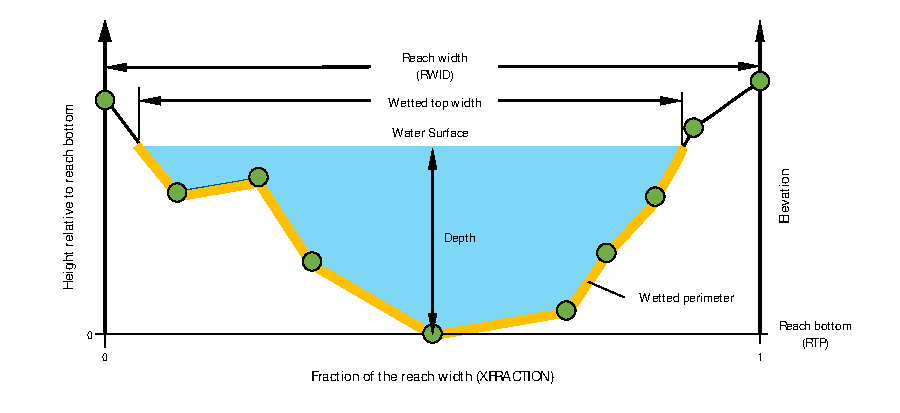
\includegraphics[scale=1.0]{../Figures/n-point-cross-section}
	\caption[Illustration of a irregular cross section used to compute depth, wetted top width, wetted perimeter, and wetted cross-sectional area for a stream reach]{Irregular cross section used to compute depth, wetted top width, wetted perimeter, and wetted cross-sectional area for a stream reach for the case where the maximum XFRACTION is one}
	\label{fig:sfr-n-point}
\end{figure}

Cross-Section tables are specified by including file names in the CROSSSECTIONS or PERIOD blocks of the SFR Package for specific reaches.  These file names correspond to a Streamflow Routing cross-section table input file.  The format of the Streamflow Routing cross-section table input file is described here.

\vspace{5mm}
\subsubsection{Structure of Blocks}
\vspace{5mm}

\lstinputlisting[style=blockdefinition]{./mf6ivar/tex/utl-sfrtab-dimensions.dat}
\lstinputlisting[style=blockdefinition]{./mf6ivar/tex/utl-sfrtab-table.dat}
\vspace{5mm}

\vspace{5mm}
\subsubsection{Explanation of Variables}
\begin{description}
% DO NOT MODIFY THIS FILE DIRECTLY.  IT IS CREATED BY mf6ivar.py 

\item \textbf{Block: DIMENSIONS}

\begin{description}
\item \texttt{nrow}---integer value specifying the number of rows in the reach cross-section table. There must be NROW rows of data in the TABLE block.

\item \texttt{ncol}---integer value specifying the number of columns in the reach cross-section table. There must be NCOL columns of data in the TABLE block. NCOL must be equal to 2 if MANFRACTION is not specified or 3 otherwise.

\end{description}
\item \textbf{Block: TABLE}

\begin{description}
\item \texttt{xfraction}---real value that defines the station (x) data for the cross-section as a fraction of the width (RWID) of the reach. XFRACTION must be greater than or equal to zero but can be greater than one. XFRACTION values can be used to decrease or increase the width of a reach from the specified reach width (RWID).

\item \texttt{height}---real value that is the height relative to the top of the lowest elevation of the streambed (RTP) and corresponding to the station data on the same line. HEIGHT must be greater than or equal to zero and at least one cross-section height must be equal to zero.

\item \texttt{manfraction}---real value that defines the Manning's roughness coefficient data for the cross-section as a fraction of the Manning's roughness coefficient for the reach (MAN) and corresponding to the station data on the same line. MANFRACTION must be greater than zero. MANFRACTION is applied from the XFRACTION value on the same line to the XFRACTION value on the next line. Although a MANFRACTION value is specified on the last line, any value greater than zero can be applied to MANFRACTION(NROW). MANFRACTION is only specified if NCOL is 3. If MANFRACTION is not specified, the Manning's roughness coefficient for the reach (MAN) is applied to the entire cross-section.

\end{description}


\end{description}

\subsubsection{Example Input File}
\lstinputlisting[style=inputfile]{./mf6ivar/examples/utl-sfrtab-example.dat}



\newpage
\subsection{Lake (LAK) Package}
\input{gwf/lak}

\newpage
\subsection{Unsaturated Zone Flow (UZF) Package}
\input{gwf/uzf}

\newpage
\subsection{Water Mover (MVR) Package}
The MVR Package can be used to transfer water from a provider to a receiver.  Providers are extraction wells, streamflow routing reaches, lakes and other model features that can be conceptualized as having water available.  The list of packages that can provide water to the MVR Package are:

\begin{itemize}
  \item Well Package
  \item Drain Package
  \item River Package
  \item General-Head Boundary Package
  \item Multi-Aquifer Well Package
  \item Streamflow Routing Package
  \item Unsaturated Zone Flow Package
  \item Lake Package
\end{itemize}

Receivers are package features within the model that solve a continuity equation of inflows, outflows, and change in storage.  These features include multi-aquifer wells, streamflow routing reaches, lakes, and unsaturated zone flow cells.  The list of packages that can receive water is shorter than the provider list, because the WEL, DRN, RIV, and GHB Packages do not represent a continuity equation (boundary stages or elevations are specified by the user).  Therefore, the list of packages that can act as receivers are:

\begin{itemize}
  \item Multi-Aquifer Well Package
  \item Streamflow Routing Package
  \item Unsaturated Zone Flow Package
  \item Lake Package
\end{itemize}

\noindent The program will terminate with an error if the MVR is used with an unsupported package type.

The MVR Package is based on the calculation of available water that can be moved from one package feature to another.  The equations used to determine how much water can be transferred are as follows, where $Q_P$ is the flow rate that can be supported by the provider (the available flow rate), and $Q_R$ is the actual rate of water transferred to the receiver.

\begin{enumerate}
\item A FACTOR can be specified such that 

$Q_R = \alpha Q_P$

\noindent where $\alpha$ is the factor to convert the provider flow rate to the receiver flow rate.

\item An EXCESS rate can be specified by the user as $Q_S$ such that

\[
    Q_R = 
\begin{cases}
    Q_P - Q_S, & \text{if } Q_P > Q_S \\
    0,              & \text{otherwise}
\end{cases}
\]

\noindent In the EXCESS case, any water that exceeds the user specified rate is provided to the receiver.  No water is provided to the receiver if the available water is less than the user specified value.

\item A THRESHOLD rate can be specified for $Q_S$ such that

\[
    Q_R = 
\begin{cases}
    0, & \text{if } Q_S > Q_P \\
    Q_S,              & \text{otherwise}
\end{cases}
\]

\noindent In the THRESHOLD case, no flow is provided to the receiver until the available water exceeds the user specified $Q_S$ rate.  Once the available water exceeds the user specified rate, then the $Q_S$ rate is provided to the receiver.

\item An UPTO rate can be specified for $Q_S$ such that

\[
    Q_R = 
\begin{cases}
    Q_S, & \text{if } Q_P > Q_S \\
    Q_P,              & \text{otherwise}
\end{cases}
\]

\noindent In the UPTO case, all of the available water will be taken from the provider up to the $Q_S$ value specified by the user.  Once $Q_S$ is exceeded, the receiver will continue to get the $Q_S$ value specified by the user.
\end{enumerate}

\noindent In the MVR PERIOD block (as shown below), the user assigns the equation used for each individual entry by specifying FACTOR, EXCESS, THRESHOLD, or UPTO to the input variable \texttt{mvrtype}.

Input to the Water Mover (MVR) Package is read from the file that has type ``MVR6'' in the Name File.  Only one MVR Package can be used per GWF Model.

\vspace{5mm}
\subsubsection{Structure of Blocks}
\vspace{5mm}

\noindent \textit{FOR EACH SIMULATION}
\lstinputlisting[style=blockdefinition]{./mf6ivar/tex/gwf-mvr-options.dat}
\lstinputlisting[style=blockdefinition]{./mf6ivar/tex/gwf-mvr-dimensions.dat}
\lstinputlisting[style=blockdefinition]{./mf6ivar/tex/gwf-mvr-packages.dat}
\vspace{5mm}
\noindent \textit{FOR ANY STRESS PERIOD}
\lstinputlisting[style=blockdefinition]{./mf6ivar/tex/gwf-mvr-period.dat}
All of the mover information in the PERIOD block will continue to apply for subsequent stress periods until the end of the simulation, or until another PERIOD block is encountered.  When a new PERIOD block is encountered, all of the movers from the previous block are replaced with the movers in the new PERIOD block.  Note that this behavior is different from the other advanced packages (MAW, SFR, LAK, and UZF).  To turn off all of the movers for a stress period, a PERIOD block must be specified with no entries.  If a PERIOD block is not specified for the first stress period, then no movers will be applied until the \texttt{iper} value of the first PERIOD block in the file.


\vspace{5mm}
\subsubsection{Explanation of Variables}
\begin{description}
\input{./mf6ivar/tex/gwf-mvr-desc.tex}
\end{description}

\vspace{5mm}
\subsubsection{Example Input File}
\lstinputlisting[style=inputfile]{./mf6ivar/examples/gwf-mvr-example.dat}


\newpage
\subsection{Ghost-Node Correction (GNC) Package}
\input{gwf/gnc}

\newpage
\subsection{Groundwater Flow (GWF) Exchange}
Input to the Groundwater Flow (GWF-GWF) Exchange is read from the file that has type ``GWF6-GWF6'' in the Simulation Name File.

The XT3D capability, which can be used to improve the accuracy of the flow calculation for certain types of cell connections and to represent anisotropic groundwater flow, is not implemented for the GWF-GWF Exchange.

\vspace{5mm}
\subsubsection{Structure of Blocks}
\lstinputlisting[style=blockdefinition]{./mf6ivar/tex/exg-gwfgwf-options.dat}
\lstinputlisting[style=blockdefinition]{./mf6ivar/tex/exg-gwfgwf-dimensions.dat}
\lstinputlisting[style=blockdefinition]{./mf6ivar/tex/exg-gwfgwf-exchangedata.dat}

\vspace{5mm}
\subsubsection{Explanation of Variables}
\begin{description}
\input{./mf6ivar/tex/exg-gwfgwf-desc.tex}
\end{description}

\vspace{5mm}
\subsubsection{Example Input File}
\lstinputlisting[style=inputfile]{./mf6ivar/examples/exg-gwfgwf-example.dat}

\vspace{5mm}
\subsubsection{Available observation types}
GWF-GWF Exchange observations include the simulated flow for any exchange (\texttt{flow-ja-face}). The data required for each GWF-GWF Exchange observation type is defined in table~\ref{table:gwf-gwfobstype}. For \texttt{flow-ja-face} observation types, negative and positive values represent a loss from and gain to the first model specified for this exchange.

\begin{longtable}{p{2cm} p{2.75cm} p{2cm} p{1.25cm} p{7cm}}
\caption{Available GWF-GWF Exchange observation types} \tabularnewline

\hline
\hline
\textbf{Exchange} & \textbf{Observation type} & \textbf{ID} & \textbf{ID2} & \textbf{Description} \\
\hline
\endhead

\hline
\endfoot

GWF-GWF & flow-ja-face & exchange number or boundname & -- & Flow between model 1 and model 2 for a specified exchange (which is the consecutive exchange number listed in the EXCHANGEDATA block), or the sum of these exchange flows by boundname if boundname is specified.
\label{table:gwf-gwfobstype}
\end{longtable}


\vspace{5mm}
\subsubsection{Example Observation Input File}
\lstinputlisting[style=inputfile]{./mf6ivar/examples/exg-gwfgwf-example-obs.dat}





%GWT Model Input Instructions
\newpage
\SECTION{Groundwater Transport (GWT) Model Input}
The GWT Model simulates three-dimensional transport of a single solute species in flowing groundwater \citep{modflow6gwt}.  The GWT Model solves the solute transport equation using numerical methods and a generalized control-volume finite-difference approach, which can be used with regular MODFLOW grids (DIS Package) or with unstructured grids (DISV and DISU Packages).  The GWT Model is designed to work with most of the new capabilities released with the GWF Model, including the Newton flow formulation, unstructured grids, advanced packages, and the movement of water between packages.  The GWF and GWT Models operate simultaneously during a \mf simulation to represent coupled groundwater flow and solute transport.  The GWT Model can also run separately from a GWF Model by reading the heads and flows saved by a previously run GWF Model.  The GWT model is also capable of working with the flows from another groundwater flow model, as long as the flows from that model can be written in the correct form to flow and head files.  

The purpose of the GWT Model is to calculate changes in solute concentration in both space and time.  Solute concentrations within an aquifer can change in response to multiple solute transport processes.  These processes include (1) advective transport of solute with flowing groundwater, (2) the combined hydrodynamic dispersion processes of velocity-dependent mechanical dispersion and chemical diffusion, (3) sorption of solutes by the aquifer matrix either by adsorption to individual solid grains or by absorption into solid grains, (4) transfer of solute into very low permeability aquifer material (called an immobile domain) where it can be stored and later released, (5) first- or zero-order solute decay or production in response to chemical or biological reactions, (6) mixing with fluids from groundwater sources and sinks, and (7) direct addition of solute mass.

With the present implementation, there can be multiple domains and multiple phases.  There is a single mobile domain, which normally consists of flowing groundwater, and there can be one or more immobile domains.  The GWT Model simulates the dissolved phase of chemical constituents in both the mobile and immobile domains.  The dissolved phase is also referred to in this report as the aqueous phase.  If sorption is represented, then the GWT Model also simulates the solid phase of the chemical constituent in both the mobile and immobile domains.  The dissolved and solid phases of the chemical constituent are tracked in the different domains by the GWT Model and can be reported as output as requested by the user.

This section describes the data files for a \mf Groundwater Transport (GWT) Model.  A GWT Model is added to the simulation by including a GWT entry in the MODELS block of the simulation name file.  There are three types of spatial discretization approaches that can be used with the GWT Model: DIS, DISV, and DISU.  The input instructions for these three packages are not described here in this section on GWT Model input; input instructions for these three packages are described in the section on GWF Model input.

The GWT Model is designed to permit input to be gathered, as it is needed, from many different files.  Likewise, results from the model calculations can be written to a number of output files. The GWT Model Listing File is a key file to which the GWT model output is written.  As \mf runs, information about the GWT Model is written to the GWT Model Listing File, including much of the input data (as a record of the simulation) and calculated results.  Details about the files used by each package are provided in this section on the GWT Model Instructions.

The GWT Model reads a file called the Name File, which specifies most of the files that will be used in a simulation. Several files are always required whereas other files are optional depending on the simulation. The Output Control Package receives instructions from the user to control the amount and frequency of output.  Details about the Name File and the Output Control Package are described in this section.

For the GWT Model, ``flows'' (unless stated otherwise) represent solute mass ``flow'' in mass per time, rather than groundwater flow.  

\subsection{Information for Existing Solute Transport Modelers}
The \mf GWT Model contains most of the functionality of MODFLOW-GWT, MT3DMS, MT3D-USGS and MODFLOW-USG.  The following list summarizes major differences between the GWT Model in \mf and previous MODFLOW-based solute transport programs.

\begin{enumerate}

\item The GWT Model simulates transport of a single chemical species; however, because \mf allows for multiple models of the same type to be included in a single simulation, multiple species can be represented by using multiple GWT Models.

\item For most simulations, the GWT Model needs groundwater flows for every cell in the model grid, for all boundary conditions, for all advanced package flow terms, and for other terms, such as the flow of water in or out of storage.  The GWT Model can access these flows in a GWF Model that is running in the same simulation as the GWT Model.  Alternatively, the GWT Model can read binary head and budget files created from a previous GWF Model simulation (provided these files contain all of the required information for all time steps); there is no specialized flow and transport link file \citep{zheng2001modflow} as there is for MT3D.  Details on these two different use cases are provided in the chapter on the FMI Package.

\item The GWT Model is based on a generalized control-volume finite-difference method, which means that solute transport can be simulated using regular MODFLOW grids consisting of layers, rows, and columns, or solute transport can be simulated using unstructured grids.

\item Advection can be simulated using central-in-space weighting, upstream weighting, or an implicit second-order TVD scheme.  The GWT model does not have the Method of Characteristics (particle-based approaches) or an explicit TVD scheme.  Consequently, the GWT Model may require a higher level of spatial discretization than other transport models that use higher order terms for advection dominated systems.  This can be an important limitation for some problems, which require the preservation of sharp solute fronts. 

\item Variable-density flow and transport can be simulated by including a GWF Model and a GWT Model in the same \mf simulation.  The Buoyancy Package should be activated for the GWF Model so that fluid density is calculated as a function of simulated concentration.  If more than one chemical species is represented then the Buoyancy Package allows the simulated concentration for each of them to be used in the density equation of state.   \cite{langevin2020hydraulic} describe the hydraulic-head formation that is implemented in the Buoyancy Package for variable-density groundwater flow and present the results from \mf variable-density simulations.  The variable-density capabilities available in \mf replicate and extend the capabilities available in SEAWAT to include the Newton flow formulation and unstructured grids, for example.  

\item The GWT Model has a Source and Sink Mixing (SSM) Package for representing the effects of GWF stress package inflows and outflows on simulated concentrations.  There are two ways in which users can assign concentrations to the individual features in these stress package.  The first way is to activate a concentration auxiliary variable in the corresponding GWF stress package.  In the SSM input file, the user provides the name of the auxiliary variable to be used for concentration.  The second way is to create a special SPC file, which contains user-assigned time-varying concentrations for stress package features.

\item The GWT model includes the MST and IST Packages.  These two package collectively comprise the capabilities of the MT3DMS Reactions Package.

\item The MST Package contains the linear, Freundlich, and Langmuir isotherms for representing sorption.  The IST Packages contains only the linear isotherm for representation of sorption. 

\item The GWT model was designed so that the user can specify as many immobile domains and necessary to represent observed contaminant transport patterns and solute breakthrough curves.  The effects of an immobile domain are represented using the Immobile Storage and Transfer (IST) Package, and the user can specify as many IST Packages as necessary.  

\item A GWT-GWT Exchange (introduced in version 6.3.0) can be used to tightly couple multiple transport models, as might be done in a nested grid configuration.  

\item There is no option to automatically run the GWT Model to steady state using a single time step.  This is an option available in MT3DMS \citep{zheng2010supplemental}.  Steady state conditions must be determined by running the transport model under transient conditions until concentrations stabilize.

\item The GWT Model described in this report is capable of simulating solute transport in the advanced stress packages of \mf, including the Lake, Streamflow Routing, Multi-Aquifer Well, Unsaturated Zone Transport Packages, and the Water Mover Package.  The present implementation simulates solute advection between package features, such as between two stream reaches, but dispersive transport is not represented.  Likewise, solute transport between the advanced packages and the aquifer occurs only through advection.

\item The GWT Model has not yet been programmed to work with the Skeletal Storage, Compaction, and Subsidence (CSUB) Package for the GWF Model.  

\item There are many other differences between the \mf GWT Model and other solute transport models that work with MODFLOW, especially with regards to program design and input and output.  Descriptions for the GWT input and output are described here.

\end{enumerate}

\subsection{Units of Length and Time}
The GWF Model formulates the groundwater flow equation without using prescribed length and time units. Any consistent units of length and time can be used when specifying the input data for a simulation. This capability gives a certain amount of freedom to the user, but care must be exercised to avoid mixing units.  The program cannot detect the use of inconsistent units.

\subsection{Solute Mass Budget}
A summary of all inflow (sources) and outflow (sinks) of solute mass is called a mass budget.  \mf calculates a mass budget for the overall model as a check on the acceptability of the solution, and to provide a summary of the sources and sinks of mass to the flow system.  The solute mass budget is printed to the GWT Model Listing File for selected time steps.

\subsection{Time Stepping}

For the present implementation of the GWT Model, all terms in the solute transport equation are solved implicitly.  With the implicit approach applied to the transport equation, it is possible to take relatively large time steps and efficiently obtain a stable solution.  If the time steps are too large, however, accuracy of the model results will suffer, so there is usually some compromise required between the desired level of accuracy and length of the time step.  An assessment of accuracy can be performed by simply running simulations with shorter time steps and comparing results.

In \mf time step lengths are controlled by the user and specified in the Temporal Discretization (TDIS) input file.  When the flow model and transport model are included in the same simulation, then the length of the time step specified in TDIS is used for both models.  If the GWT Model runs in a separate simulation from the GWT Model, then the time steps used for the transport model can be different, and likely shorter, than the time steps used for the flow solution.  Instructions for specifying time steps are described in the TDIS section of this user guide; additional information on GWF and GWT configurations are in the Flow Model Interface section.  



\newpage
\subsection{GWT Model Name File}
The GWE Model Name File specifies the options and packages that are active for a GWE model.  The Name File contains two blocks: OPTIONS  and PACKAGES. The length of each line must be 299 characters or less. The lines in each block can be in any order.  Files listed in the PACKAGES block must exist when the program starts. 

Comment lines are indicated when the first character in a line is one of the valid comment characters.  Commented lines can be located anywhere in the file. Any text characters can follow the comment character. Comment lines have no effect on the simulation; their purpose is to allow users to provide documentation about a particular simulation. 

\vspace{5mm}
\subsubsection{Structure of Blocks}
\lstinputlisting[style=blockdefinition]{./mf6ivar/tex/gwe-nam-options.dat}
\lstinputlisting[style=blockdefinition]{./mf6ivar/tex/gwe-nam-packages.dat}

\vspace{5mm}
\subsubsection{Explanation of Variables}
\begin{description}
\input{./mf6ivar/tex/gwe-nam-desc.tex}
\end{description}

\begin{table}[H]
\caption{Ftype values described in this report.  The \texttt{Pname} column indicates whether or not a package name can be provided in the name file.  The capability to provide a package name also indicates that the GWE Model can have more than one package of that Ftype}
\small
\begin{center}
\begin{tabular*}{\columnwidth}{l l l}
\hline
\hline
Ftype & Input File Description & \texttt{Pname}\\
\hline
DIS6 & Rectilinear Discretization Input File \\
DISV6 & Discretization by Vertices Input File \\
DISU6 & Unstructured Discretization Input File \\
FMI6 & Flow Model Interface Package &  \\ 
IC6 & Initial Conditions Package \\
OC6 & Output Control Option \\
ADV6 & Advection Package \\ 
CND6 & Conduction and Dispersion Package \\ 
SSM6 & Source and Sink Mixing Package \\ 
EST6 & Energy Storage and Transfer Package \\
CTP6 & Constant Temperature Package & * \\ 
ESL6 & Energy Source Loading Package & * \\
SFE6 & Streamflow Energy Transport Package & * \\
LKE6 & Lake Energy Transport Package & * \\
MWE6 & Multi-Aquifer Well Energy Transport Package & * \\
UZE6 & Unsaturated-Zone Energy Transport Package & * \\
MVE6 & Mover Energy Transport Package \\
OBS6 & Observations Option \\
\hline 
\end{tabular*}
\label{table:ftype-gwe}
\end{center}
\normalsize
\end{table}

\vspace{5mm}
\subsubsection{Example Input File}
\lstinputlisting[style=inputfile]{./mf6ivar/examples/gwe-nam-example.dat}



%\newpage
%\subsection{Structured Discretization (DIS) Input File}
%\input{gwf/dis}

%\newpage
%\subsection{Discretization with Vertices (DISV) Input File}
%\input{gwf/disv}

%\newpage
%\subsection{Unstructured Discretization (DISU) Input File}
%\input{gwf/disu}

\newpage
\subsection{Initial Conditions (IC) Package}
Initial Conditions (IC) Package information is read from the file that is specified by ``IC6'' as the file type.  Only one IC Package can be specified for a GWF model. 

\vspace{5mm}
\subsubsection{Structure of Blocks}
\lstinputlisting[style=blockdefinition]{./mf6ivar/tex/gwf-ic-options.dat}
\lstinputlisting[style=blockdefinition]{./mf6ivar/tex/gwf-ic-griddata.dat}

\vspace{5mm}
\subsubsection{Explanation of Variables}
\begin{description}
\input{./mf6ivar/tex/gwf-ic-desc.tex}
\end{description}

\vspace{5mm}
\subsubsection{Example Input File}
\lstinputlisting[style=inputfile]{./mf6ivar/examples/gwf-ic-example.dat}



\newpage
\subsection{Output Control (OC) Option}
Input to the Output Control Option of the Groundwater Energy Transport Model is read from the file that is specified as type ``OC6'' in the Name File. If no ``OC6'' file is specified, default output control is used. The Output Control Option determines how and when temperatures are printed to the listing file and/or written to a separate binary output file.  Under the default, temperature and the overall energy transport budget are written to the Listing File at the end of every stress period. The default printout format for temperatures is 10G11.4.  The temperatures and overall energy transport budget are also written to the list file if the simulation terminates prematurely due to failed convergence.

Output Control data must be specified using words.  The numeric codes supported in earlier MODFLOW versions can no longer be used.

For the PRINT and SAVE options of temperature, there is no option to specify individual layers.  Whenever the temperature array is printed or saved, all layers are printed or saved.

\vspace{5mm}
\subsubsection{Structure of Blocks}
\vspace{5mm}

\noindent \textit{FOR EACH SIMULATION}
\lstinputlisting[style=blockdefinition]{./mf6ivar/tex/gwe-oc-options.dat}
\vspace{5mm}
\noindent \textit{FOR ANY STRESS PERIOD}
\lstinputlisting[style=blockdefinition]{./mf6ivar/tex/gwe-oc-period.dat}

\vspace{5mm}
\subsubsection{Explanation of Variables}
\begin{description}
\input{./mf6ivar/tex/gwe-oc-desc.tex}
\end{description}

\vspace{5mm}
\subsubsection{Example Input File}
\lstinputlisting[style=inputfile]{./mf6ivar/examples/gwe-oc-example.dat}


\newpage
\subsection{Observation (OBS) Utility for a GWT Model}
\input{gwt/gwt-obs}

\newpage
\subsection{Advection (ADV) Package}
Advection (ADV) Package information is read from the file that is specified by ``ADV6'' as the file type.  Only one ADV Package can be specified for a GWE model. 

\vspace{5mm}
\subsubsection{Structure of Blocks}
\lstinputlisting[style=blockdefinition]{./mf6ivar/tex/gwe-adv-options.dat}

\vspace{5mm}
\subsubsection{Explanation of Variables}
\begin{description}
\input{./mf6ivar/tex/gwe-adv-desc.tex}
\end{description}

\vspace{5mm}
\subsubsection{Example Input File}
\lstinputlisting[style=inputfile]{./mf6ivar/examples/gwe-adv-example.dat}



\newpage
\subsection{Dispersion (DSP) Package}
Dispersion (DSP) Package information is read from the file that is specified by ``DSP6'' as the file type.  Only one DSP Package can be specified for a GWT model.  By default, the DSP Package uses the mathematical formulation presented for the XT3D option of the NPF Package to represent full three-dimensional anisotropy in groundwater flow.  XT3D can be computationally expensive and can be turned off to use a simplified and approximate form of the dispersion equations.  For most problems, however, XT3D will be required to accurately represent dispersion.

\vspace{5mm}
\subsubsection{Structure of Blocks}
\lstinputlisting[style=blockdefinition]{./mf6ivar/tex/gwt-dsp-options.dat}
\lstinputlisting[style=blockdefinition]{./mf6ivar/tex/gwt-dsp-griddata.dat}

\vspace{5mm}
\subsubsection{Explanation of Variables}
\begin{description}
\input{./mf6ivar/tex/gwt-dsp-desc.tex}
\end{description}

\vspace{5mm}
\subsubsection{Example Input File}
\lstinputlisting[style=inputfile]{./mf6ivar/examples/gwt-dsp-example.dat}



\newpage
\subsection{Source and Sink Mixing (SSM) Package}
Source and Sink Mixing (SSM) Package information is read from the file that is specified by ``SSM6'' as the file type.  Only one SSM Package can be specified for a GWE model.  The SSM Package is required if the flow model has any stress packages.

The SSM Package is used to add or remove thermal energy from GWE model cells based on inflows and outflows from GWF stress packages.  If a GWF stress package provides flow into a model cell, that flow can be assigned a user-specified temperature.  If a GWF stress package removes water from a model cell, the temperature of that water is the temperature of the cell from which the water is removed.  For flow boundary conditions that include evapotranspiration, the latent heat of vaporization may be used to represent evaporative cooling.  There are several different ways for the user to specify the temperatures.  

\begin{itemize}
\item The default condition is that sources have a temperature of zero and sinks withdraw water at the calculated temperature of the cell.  This default condition is assigned to any GWF stress package that is not included in a SOURCES block or FILEINPUT block.
\item A second option is to assign auxiliary variables in the GWF model and include a temperature for each stress boundary.  In this case, the user provides the name of the package and the name of the auxiliary variable containing temperature values for each boundary.  As described below for srctype, there are multiple options for defining this behavior.
\item A third option is to prepare an input file using the \hyperref[sec:spc]{Stress Package Component (SPC6) utility} for any desired GWF stress package.  This SPC6 file allows users to change temperatures by stress period, or to use the time-series option to interpolate temperatures by time step.  This third option was introduced in MODFLOW version 6.3.0.  Information for this approach is entered in an optional FILEINPUT block below.  The SPC6 input file supports list-based temperature input for most corresponding GWF stress packages, but also supports a READASARRAYS array-based input format if a corresponding GWF recharge or evapotranspiration package uses the READASARRAYS option.
\end{itemize}

\noindent The auxiliary method and the SPC6 file input method can both be used for a GWE model, but only one approach can be assigned per GWF stress package.   If a flow package specified in the SOURCES or FILEINPUT blocks is also represented using an advanced transport package (SFE, LKE, MWE, or UZE), then the advanced transport package will override SSM calculations for that package.

\vspace{5mm}
\subsubsection{Structure of Blocks}
\lstinputlisting[style=blockdefinition]{./mf6ivar/tex/gwe-ssm-options.dat}
\lstinputlisting[style=blockdefinition]{./mf6ivar/tex/gwe-ssm-sources.dat}
\vspace{5mm}
\noindent \textit{FILEINPUT BLOCK IS OPTIONAL}
\lstinputlisting[style=blockdefinition]{./mf6ivar/tex/gwe-ssm-fileinput.dat}

\vspace{5mm}
\subsubsection{Explanation of Variables}
\begin{description}
\input{./mf6ivar/tex/gwe-ssm-desc.tex}
\end{description}

\vspace{5mm}
\subsubsection{Example Input File}
\lstinputlisting[style=inputfile]{./mf6ivar/examples/gwe-ssm-example.dat}

% when obs are ready, they should go here




\newpage
\subsection{Mobile Storage and Transfer (MST) Package}
\input{gwt/mst}

\newpage
\subsection{Immobile Storage and Transfer (IST) Package}
Immobile Storage and Transfer (IST) Package information is read from the file that is specified by ``IST6'' as the file type.  Any number of IST Packages can be specified for a single GWT model.  This allows the user to specify triple porosity systems, or systems with as many immobile domains as necessary. 

Subsequent to MODFLOW Version 6.4.1, substantial changes were made to the input parameter definitions and conceptualization of the IST Package.  These changes are described in Chapter 9 of the MODFLOW 6 Supplemental Technical Information document that is included with the distribution.

\vspace{5mm}
\subsubsection{Structure of Blocks}
\lstinputlisting[style=blockdefinition]{./mf6ivar/tex/gwt-ist-options.dat}
\lstinputlisting[style=blockdefinition]{./mf6ivar/tex/gwt-ist-griddata.dat}

\vspace{5mm}
\subsubsection{Explanation of Variables}
\begin{description}
\input{./mf6ivar/tex/gwt-ist-desc.tex}
\end{description}

\vspace{5mm}
\subsubsection{Example Input File}
\lstinputlisting[style=inputfile]{./mf6ivar/examples/gwt-ist-example.dat}



\newpage
\subsection{Constant Concentration (CNC) Package}
\input{gwt/cnc}

\newpage
\subsection{Mass Source Loading (SRC) Package}
\input{gwt/src}

\newpage
\subsection{Streamflow Transport (SFT) Package}
\input{gwt/sft}

\newpage
\subsection{Lake Transport (LKT) Package}
\input{gwt/lkt}

\newpage
\subsection{Multi-Aquifer Well Transport (MWT) Package}
\input{gwt/mwt}

\newpage
\subsection{Unsaturated Zone Transport (UZT) Package}
\input{gwt/uzt}

\newpage
\subsection{Flow Model Interface (FMI) Package}
Flow Model Interface (FMI) Package information is read from the file that is specified by ``FMI6'' as the file type.  The FMI Package file is required only if the PRT Model is running in a separate simulation from a previously run GWF Model. If the PRT Model is coupled to a GWF Model by an exchange, the FMI Package file is not required. Only one FMI Package can be specified for a PRT model.

The PRT Model needs groundwater flows for model grid cells, for boundary conditions, and for other terms, such as the flow of water in or out of storage.  The FMI Package is the interface between the PRT Model and simulated groundwater flows provided by a corresponding GWF Model that is running concurrently within the simulation or from binary budget files that were created from a previous GWF model run.  The following are several different FMI simulation cases:

\begin{itemize}

\item Flows are provided by a corresponding GWF Model running in the same simulation---in this case, all groundwater flows are calculated by the corresponding GWF Model and provided through FMI to the transport model.  This is a common use case in which the user wants to run the flow and particle-tracking models as part of a single simulation.  The GWF and PRT models must be part of a GWF-PRT Exchange that is listed in mfsim.nam.  If a GWF-PRT Exchange is specified by the user, then the user does not need to specify an FMI Package input file for the simulation, unless an FMI option is needed.  If a GWF-PRT Exchange is specified and the FMI Package is specified, then the PACKAGEDATA block below is not read or used.

\item Flows are provided from a previous GWF model simulation---in this case FMI should be provided in the PRT name file and the head and budget files should be listed in the FMI PACKAGEDATA block.  In this case, FMI reads the simulated head and flows from these files and makes them available to the particle-tracking model.  There are some additional considerations when the heads and flows are provided from binary files.

\begin{itemize}
\item The binary budget file must contain the simulated flows for all of the packages that were included in the GWF model run.  Saving of flows can be activated for all packages by specifying ``SAVE\_FLOWS'' as an option in the GWF name file.  The GWF Output Control Package must also have ``SAVE BUDGET ALL'' specified.  The easiest way to ensure that all flows and heads are saved is to use the following simple form of a GWF Output Control file:

\begin{verbatim}
BEGIN OPTIONS
  HEAD FILEOUT mymodel.hds
  BUDGET FILEOUT mymodel.bud
END OPTIONS

BEGIN PERIOD 1
  SAVE HEAD ALL
  SAVE BUDGET ALL
END PERIOD
\end{verbatim}

\item The binary budget file must have the same number of budget terms listed for each time step.  This will always be the case when the binary budget file is created by \mf.
\item The binary heads file must have heads saved for all layers in the model.  This will always be the case when the binary head file is created by \mf.  This was not always the case as previous MODFLOW versions allowed different save options for each layer.
\item If the binary budget and head files have more than one time step for a single stress period, then the budget and head information must be contained within the binary file for every time step in the simulation stress period.
\item The binary budget and head files must correspond in terms of information stored for each time step and stress period.
\item If the binary budget and head files have information provided for only the first time step of a given stress period, this information will be used for all time steps in that stress period in the PRT simulation. If the final (or only) stress period in the binary budget and head files contains data for only one time step, this information will be used for any subsequent time steps and stress periods in the PRT simulation. This makes it possible to provide flows, for example, from a steady-state GWF stress period and have those flows used for all PRT time steps in that stress period, for all remaining time steps in the PRT simulation, or for all time steps throughout the entire PRT simulation. With this option, it is possible to have smaller time steps in the PRT simulation than the time steps used in the GWF simulation. Note that this cannot be done when the GWF and PRT models are run in the same simulation, because in that case, both models are solved over the same sequence of time steps and stress periods, as listed in the TDIS Package. The option to read flows from a previous GWF simulation via Flow Model Interface may offer an efficient alternative to running both models in the same simulation, but comes at the cost of having potentially very large budget files.
\item The binary grid file is optional but recommended, as it allows \mf to verify that the GWF and PRT model grids are identical.
\end{itemize}

\end{itemize}

\noindent Determination of which FMI use case to invoke requires careful consideration of the different advantages and disadvantages of each case.  For example, running PRT and GWF in the same simulation can often be faster because GWF flows are passed through memory to the PRT model instead of being written to files.  The disadvantage of this approach is that the same time step lengths must be used for both GWF and PRT.  Ultimately, it should be relatively straightforward to test different ways in which GWF and PRT interact and select the use case most appropriate for the particular problem. 

\vspace{5mm}
\subsubsection{Structure of Blocks}
\lstinputlisting[style=blockdefinition]{./mf6ivar/tex/prt-fmi-packagedata.dat}

\vspace{5mm}
\subsubsection{Explanation of Variables}
\begin{description}
\input{./mf6ivar/tex/prt-fmi-desc.tex}
\end{description}

\vspace{5mm}
\subsubsection{Example Input File}
\lstinputlisting[style=inputfile]{./mf6ivar/examples/prt-fmi-example.dat}



\newpage
\subsection{Mover Transport (MVT) Package}
\input{gwt/mvt}

\newpage
\subsection{Groundwater Transport (GWT) Exchange}
Input to the Groundwater Transport (GWT-GWT) Exchange is read from the file that has type ``GWT6-GWT6'' in the Simulation Name File.

The list of exchanges entered into the EXCHANGEDATA block must be identical to the list of exchanges entered for the GWF-GWF input file.  One way to ensure that this information is identical is to put this list into an external file and refer to this same list using the OPEN/CLOSE functionality in both this EXCHANGEDATA input block and the EXCHANGEDATA input block in the GWF-GWF input file.

\vspace{5mm}
\subsubsection{Structure of Blocks}
\lstinputlisting[style=blockdefinition]{./mf6ivar/tex/exg-gwtgwt-options.dat}
\lstinputlisting[style=blockdefinition]{./mf6ivar/tex/exg-gwtgwt-dimensions.dat}
\lstinputlisting[style=blockdefinition]{./mf6ivar/tex/exg-gwtgwt-exchangedata.dat}

\vspace{5mm}
\subsubsection{Explanation of Variables}
\begin{description}
\input{./mf6ivar/tex/exg-gwtgwt-desc.tex}
\end{description}

\vspace{5mm}
\subsubsection{Example Input File}
\lstinputlisting[style=inputfile]{./mf6ivar/examples/exg-gwtgwt-example.dat}

\vspace{5mm}
\subsubsection{Available observation types}
GWT-GWT Exchange observations include the simulated flow for any exchange (\texttt{flow-ja-face}). The data required for each GWT-GWT Exchange observation type is defined in table~\ref{table:gwt-gwtobstype}. For \texttt{flow-ja-face} observation types, negative and positive values represent a loss from and gain to the first model specified for this exchange.

\begin{longtable}{p{2cm} p{2.75cm} p{2cm} p{1.25cm} p{7cm}}
\caption{Available GWT-GWT Exchange observation types} \tabularnewline

\hline
\hline
\textbf{Exchange} & \textbf{Observation type} & \textbf{ID} & \textbf{ID2} & \textbf{Description} \\
\hline
\endhead

\hline
\endfoot

GWT-GWT & flow-ja-face & exchange number or boundname & -- & Mass flow between model 1 and model 2 for a specified exchange (which is the consecutive exchange number listed in the EXCHANGEDATA block), or the sum of these exchange flows by boundname if boundname is specified.
\label{table:gwt-gwtobstype}
\end{longtable}


\vspace{5mm}
\subsubsection{Example Observation Input File}
\lstinputlisting[style=inputfile]{./mf6ivar/examples/exg-gwtgwt-example-obs.dat}





%GWE Model Input Instructions
\newpage
\SECTION{Groundwater Energy Transport (GWE) Model Input}
Like GWT \citep{modflow6gwt}, the GWE Model simulates three-dimensional transport in flowing groundwater.  The primary difference between GWT and GWE is that heat (i.e., temperature), instead of concentration, is the simulated ``species.'' As such, the GWE Model solves the heat transport equation using numerical methods and a generalized control-volume finite-difference approach, which can be used with regular MODFLOW grids (DIS Package) or with unstructured grids (DISV and DISU Packages).  The GWE Model is designed to work with most of the new capabilities released with the GWF Model, including the Newton flow formulation, XT3D \citep{modflow6xt3d}, unstructured grids, advanced packages, and the movement of water between packages.  The GWF and GWE (and, if active, GWT) models operate simultaneously during a \mf simulation to represent coupled groundwater flow and heat transport.  The GWE Model can also run separately from a GWF Model by reading the heads and flows saved by a previously run GWF Model.  The GWE model is also capable of working with the flows from another groundwater flow model as long as the cell-by-cell and boundary flows and groundwater heads are written to ``linker'' files in the correct format.  

The purpose of the GWE Model is to calculate changes in groundwater temperature in both space and time.  Groundwater temperature within an aquifer can change in response to different energy transport processes.  These processes include (1) convective (advective) transport of heat with flowing groundwater, (2) the combined hydrodynamic dispersion processes of velocity-dependent mechanical dispersion and conduction (analogous to chemical diffusion), (3) thermal equilibrium with the aquifer matrix, (4) mixing of fluids from groundwater sources and sinks, and (5) direct addition of thermal energy.

For GWE, the temperature at any point in the aquifer is assumed to instantaneously equilibrate between the aqueous and solid phase domains.  For example, a pulse of heat convecting through an aquifer will be retarded through thermal equilibration with the aquifer material.  Conversely, the introduction of cold groundwater into a previously warm region of the aquifer will warm up, at least in part, as energy within the aquifer matrix transfers to the aqueous phase.  Unlike GWT, the GWE Model type does not support an immobile domain.  The energy that is transferred between the aqeous and solid phases of the groundwater system are tracked in the GWE Model budget.

This section describes the data files for a \mf Groundwater Energy Transport (GWE) Model.  A GWE Model is added to the simulation by including a GWE entry in the MODELS block of the simulation name file.  There are three types of spatial discretization approaches that can be used with the GWE Model: DIS, DISV, and DISU.  The input instructions for these three packages are not described here in this section on GWE Model input; input instructions for these three packages are described in the section on GWF Model input.

The GWE Model is designed to permit input to be gathered, as it is needed, from many different files.  Likewise, results from the model calculations can be written to a number of output files. The GWE Model Listing File is a key file to which the GWE model output is written.  As \mf runs, information about the GWE Model is written to the GWE Model Listing File, including much of the input data (as a record of the simulation) and calculated results.  Details about the files used by each package are provided in this section.

The GWE Model reads a file called the Name File, which specifies most of the files that will be used in a groundwater energy transport simulation. Several files are always required whereas other files are optional depending on the question(s) being addressed by the model. The Output Control Package receives instructions from the user to control the amount and frequency of output.  Details about the Name File and the Output Control Package are described in this section.

For the GWE Model, ``flows'' (unless stated otherwise) represent the ``flow'' of energy, often expressed in units of energy (e.g., joules) per time, rather than groundwater flow.  

\subsection{Information for Existing Heat Transport Modelers}
An important goal of the \mf GWE Model is to alleviate the need for ``parameter equivalents'' when simulating heat transport in groundwater systems.  In the past, codes like HST3D \citep{kipp1987} or VS2DH \citep{healy1996} simulated energy transport directly by supporting the use of native heat transport units.  For example, users could directly specify thermal conductivity of the fluid and solid phases, as well as the heat capacity of both phases.  Alternatively, codes like MT3DMS \citep{zheng1999mt3dms}, MT3D-USGS \citep{mt3dusgs}, and MODFLOW-USG \citep{modflowusg} could be used to simulate the movement of heat in groundwater, but required users to leverage existing variables as surrogates for heat transport.  For example, the molecular diffusion parameter may be used as a surrogate for simulating thermal conduction in an aquifer \citep{mazheng2010, hechtmendez}. 

The following list summarizes important aspects of GWE for simulating heat transport with \mf:

\begin{enumerate}

\item The GWE Model uses parameters that are native to heat transport, including thermal conductivity of water, heat capacity of water, thermal conductivity of the aquifer material, heat capacity of of the aquifer material, and latent heat of vaporization. Therefore, users do not need to pre-calculate solute-transport ``parameter equivalents'' when generating GWE model input; users can instead enter native parameter values that are readily available.

\item Thermal energy transport budgets written to the \mf list file are reported in units of energy (e.g., joules).  Previously, using a program like MT3D-USGS \citep{mt3dusgs} to emulate heat transport using solute transport, units in the list file budget did not correspond to thermal energy, but were reported in units of $\frac{m^{3 \;\circ}C}{d}$. To convert to thermal energy units, values in the list file had to be post-processed by multiplying each line item by the density of water ($\rho_w$) and the heat capacity of water ($C_p$) \citep{langevin2008seawat}.

\item Thermal equilibrium between the aqueous and solid phases is assumed.  Thus, simulated temperatures are representative of both phases.  As a result, thermal conduction between adjacent cells may still occur even in the absence of convection.

\item In GWE, dry cells (devoid of groundwater) remain active for simulating thermal conduction. For example, energy (heat) transfer will be simulated between a partially saturated cell (i.e., ``water-table'' cell) and an overlying dry cell. In this way, a more full accounting of various heat transport processes is represented in the subsurface.  Moreover, this approach readily supports heat transport in the unsaturated-zone when the UZE (unsaturated-zone energy transport) Package is active.  

\item Heat transport is supported for all five of the advanced GWF packages using the following packages in GWE: (1) streamflow energy transport, SFE Package; (2) lake energy transport, LKE Package; (3) multi-aquifer well energy transport, MWE Package; (4) unsaturated zone energy transport, UZE Package; and the (5) Water Mover Package, MVE.  Similar to GWT, GWE will simulate heat transfer between an advanced package and the groundwater system via groundwater surface-water exchange; however, GWE also simulates a conductive transfer of heat between an advanced package feature and the aquifer.  To take advantage of this functionality, users must specify the thermal conductivity of the material separating a stream from the aquifer, for example, the thermal conductivity of the streambed (or lakebed), as well as the thickness of the streambed (or lakebed).  As with the advanced GWT packages, GWE simulates thermal convection between package features, such as between two stream reaches for example.  Also, dispersive heat transport among among advanced package features is not represented, similar to GWT.

\item Where the GWF model simulates evaporation from an open body of water, for example from the surface of a stream or lake, the latent heat of vaporization may be used to simulate evaporative cooling.  As water is converted from liquid to gas, the energy required by the phase change is drawn from the remaining body of water and the resulting cool down is calculated.

\end{enumerate}

Many of the same considerations listed for the GWT model should be kept in mind when developing a GWE model. For convenience, many of those considerations are adapted for GWE and repeated here.

\begin{enumerate}

\item A GWE Model can access flows calculated by a GWF Model that is running in the same simulation as the GWE Model.  Alternatively, a GWE Model can read binary head and budget files created from a previous GWF Model simulation (provided these files contain all of the required information for all time steps); there is no specialized flow and transport link file \citep{zheng2001modflow} as there is for MT3D.  Details on these two different use cases are provided in the chapter on the FMI Package.

\item The GWE Model is based on a generalized control-volume finite-difference method, which means that heat transport can be simulated using regular MODFLOW grids consisting of layers, rows, and columns, or heat transport can be simulated using unstructured grids.

\item GWE and GWT use the same advection package source code.  As a result, advection can be simulated using central-in-space weighting, upstream weighting, or an implicit second-order TVD scheme.  Currently, neither the GWE or GWT models can use a Method of Characteristics (particle-based approaches) or an explicit TVD scheme to simulate convective (or advective) transport.  Consequently, the GWE Model may require a higher level of spatial discretization than other transport models that use higher order terms for advection dominated systems.  This can be an important limitation in problems involving sharp heat fronts. 

\item The Viscosity Package can use temperatures from the GWE model to adjust the viscosities in the flow model.   

\item GWE and GWT use the same Source and Sink Mixing (SSM) Package for representing the effects of GWF stress package inflows and outflows on simulated temperatures and concentrations.  In a GWE simulation, there are two ways in which users can assign temperatures to the individual features in these stress package.  The first way is to activate a temperature auxiliary variable in the corresponding GWF stress package.  In the SSM input file, the user provides the name of the auxiliary variable to be used for temperature.  The second way is to create a special SPC file, which contains user-assigned time-varying temperatures for stress package features.

\item The GWE model includes an Energy Storage and Transfer (EST) Package that is analogous to the MST Package in the GWT Model.  The GWE Model does not simulate immobile domains and therefore does not include an analog of the IST Package in the GWT Model.  

\item A GWE-GWE Exchange (introduced in version 6.5.0) can be used to tightly couple multiple heat transport models, as might be done in a nested grid configuration.  

\item There is no option to automatically run the GWE Model to steady state using a single time step.  This is an option available in MT3DMS \citep{zheng2010supplemental}.  Steady state conditions must be determined by running the transport model under transient conditions until temperatures stabilize.

\item As is the case with GWT, the GWE Model has not yet been programmed to work with the Skeletal Storage, Compaction, and Subsidence (CSUB) Package for the GWF Model.  

\end{enumerate}

\subsection{Units of Length and Time}
The GWE Model formulates the groundwater energy transport equation without using prescribed length and time units. Any consistent units of length and time can be used when specifying the input data for a simulation. This capability gives a certain amount of freedom to the user, but care must be exercised to avoid mixing units.  The program cannot detect the use of inconsistent units.

\subsection{Thermal Energy Budget}
A summary of all inflow (sources) and outflow (sinks) of thermal energy is referred to as an energy budget.  \mf calculates an energy budget for the overall model as a check on the acceptability of the solution, and to provide a summary of the sources and sinks of energy to the flow system.  The energy budget is printed to the GWE Model Listing File for specified time steps.

\subsection{Time Stepping}

For the present implementation of the GWE Model, all terms in the heat transport equation are solved implicitly.  With the implicit approach applied to the transport equation, it is possible to take relatively large time steps and efficiently obtain a stable solution.  If the time steps are too large, however, accuracy of the model results will suffer, so there is usually some compromise required between the desired level of accuracy and length of the time step.  An assessment of accuracy can be performed by simply running simulations with shorter time steps and comparing results.

In \mf time step lengths are controlled by the user and specified in the Temporal Discretization (TDIS) input file.  When the flow model and heat transport model are included in the same simulation, then the length of the time step specified in TDIS is used for both models.  If the GWE Model runs in a separate simulation from the GWE Model, then the time steps used for the heat transport model can be different, and likely shorter, than the time steps used for the flow solution.  Instructions for specifying time steps are described in the TDIS section of this user guide; additional information on GWF and GWE configurations are in the Flow Model Interface section.  



\newpage
\subsection{GWE Model Name File}
The GWE Model Name File specifies the options and packages that are active for a GWE model.  The Name File contains two blocks: OPTIONS  and PACKAGES. The length of each line must be 299 characters or less. The lines in each block can be in any order.  Files listed in the PACKAGES block must exist when the program starts. 

Comment lines are indicated when the first character in a line is one of the valid comment characters.  Commented lines can be located anywhere in the file. Any text characters can follow the comment character. Comment lines have no effect on the simulation; their purpose is to allow users to provide documentation about a particular simulation. 

\vspace{5mm}
\subsubsection{Structure of Blocks}
\lstinputlisting[style=blockdefinition]{./mf6ivar/tex/gwe-nam-options.dat}
\lstinputlisting[style=blockdefinition]{./mf6ivar/tex/gwe-nam-packages.dat}

\vspace{5mm}
\subsubsection{Explanation of Variables}
\begin{description}
\input{./mf6ivar/tex/gwe-nam-desc.tex}
\end{description}

\begin{table}[H]
\caption{Ftype values described in this report.  The \texttt{Pname} column indicates whether or not a package name can be provided in the name file.  The capability to provide a package name also indicates that the GWE Model can have more than one package of that Ftype}
\small
\begin{center}
\begin{tabular*}{\columnwidth}{l l l}
\hline
\hline
Ftype & Input File Description & \texttt{Pname}\\
\hline
DIS6 & Rectilinear Discretization Input File \\
DISV6 & Discretization by Vertices Input File \\
DISU6 & Unstructured Discretization Input File \\
FMI6 & Flow Model Interface Package &  \\ 
IC6 & Initial Conditions Package \\
OC6 & Output Control Option \\
ADV6 & Advection Package \\ 
CND6 & Conduction and Dispersion Package \\ 
SSM6 & Source and Sink Mixing Package \\ 
EST6 & Energy Storage and Transfer Package \\
CTP6 & Constant Temperature Package & * \\ 
ESL6 & Energy Source Loading Package & * \\
SFE6 & Streamflow Energy Transport Package & * \\
LKE6 & Lake Energy Transport Package & * \\
MWE6 & Multi-Aquifer Well Energy Transport Package & * \\
UZE6 & Unsaturated-Zone Energy Transport Package & * \\
MVE6 & Mover Energy Transport Package \\
OBS6 & Observations Option \\
\hline 
\end{tabular*}
\label{table:ftype-gwe}
\end{center}
\normalsize
\end{table}

\vspace{5mm}
\subsubsection{Example Input File}
\lstinputlisting[style=inputfile]{./mf6ivar/examples/gwe-nam-example.dat}



%\newpage
%\subsection{Structured Discretization (DIS) Input File}
%\input{gwf/dis}

%\newpage
%\subsection{Discretization with Vertices (DISV) Input File}
%\input{gwf/disv}

%\newpage
%\subsection{Unstructured Discretization (DISU) Input File}
%\input{gwf/disu}

\newpage
\subsection{Initial Conditions (IC) Package}
Initial Conditions (IC) Package information is read from the file that is specified by ``IC6'' as the file type.  Only one IC Package can be specified for a GWF model. 

\vspace{5mm}
\subsubsection{Structure of Blocks}
\lstinputlisting[style=blockdefinition]{./mf6ivar/tex/gwf-ic-options.dat}
\lstinputlisting[style=blockdefinition]{./mf6ivar/tex/gwf-ic-griddata.dat}

\vspace{5mm}
\subsubsection{Explanation of Variables}
\begin{description}
\input{./mf6ivar/tex/gwf-ic-desc.tex}
\end{description}

\vspace{5mm}
\subsubsection{Example Input File}
\lstinputlisting[style=inputfile]{./mf6ivar/examples/gwf-ic-example.dat}



\newpage
\subsection{Output Control (OC) Option}
Input to the Output Control Option of the Groundwater Energy Transport Model is read from the file that is specified as type ``OC6'' in the Name File. If no ``OC6'' file is specified, default output control is used. The Output Control Option determines how and when temperatures are printed to the listing file and/or written to a separate binary output file.  Under the default, temperature and the overall energy transport budget are written to the Listing File at the end of every stress period. The default printout format for temperatures is 10G11.4.  The temperatures and overall energy transport budget are also written to the list file if the simulation terminates prematurely due to failed convergence.

Output Control data must be specified using words.  The numeric codes supported in earlier MODFLOW versions can no longer be used.

For the PRINT and SAVE options of temperature, there is no option to specify individual layers.  Whenever the temperature array is printed or saved, all layers are printed or saved.

\vspace{5mm}
\subsubsection{Structure of Blocks}
\vspace{5mm}

\noindent \textit{FOR EACH SIMULATION}
\lstinputlisting[style=blockdefinition]{./mf6ivar/tex/gwe-oc-options.dat}
\vspace{5mm}
\noindent \textit{FOR ANY STRESS PERIOD}
\lstinputlisting[style=blockdefinition]{./mf6ivar/tex/gwe-oc-period.dat}

\vspace{5mm}
\subsubsection{Explanation of Variables}
\begin{description}
\input{./mf6ivar/tex/gwe-oc-desc.tex}
\end{description}

\vspace{5mm}
\subsubsection{Example Input File}
\lstinputlisting[style=inputfile]{./mf6ivar/examples/gwe-oc-example.dat}


\newpage
\subsection{Observation (OBS) Utility for a GWE Model}

GWE Model observations include the simulated groundwater temperature (\texttt{temperature}), and the energy flow, with units of energy per time, between two connected cells (\texttt{flow-ja-face}). The data required for each GWE Model observation type is defined in table~\ref{table:gweobstype}. For \texttt{flow-ja-face} observation types, negative and positive values represent a loss from and gain to the \texttt{cellid} specified for ID, respectively.

\subsubsection{Structure of Blocks}
\vspace{5mm}

\noindent \textit{FOR EACH SIMULATION}
\lstinputlisting[style=blockdefinition]{./mf6ivar/tex/utl-obs-options.dat}
\lstinputlisting[style=blockdefinition]{./mf6ivar/tex/utl-obs-continuous.dat}

\subsubsection{Explanation of Variables}
\begin{description}
\input{./mf6ivar/tex/utl-obs-desc.tex}
\end{description}


\begin{longtable}{p{2cm} p{2.75cm} p{2cm} p{1.25cm} p{7cm}}
\caption{Available GWE model observation types} \tabularnewline

\hline
\hline
\textbf{Model} & \textbf{Observation type} & \textbf{ID} & \textbf{ID2} & \textbf{Description} \\
\hline
\endhead

\hline
\endfoot


GWE Model observations include the simulated groundwater temperature (\texttt{temperature}), and the energy flow, with units of energy per time, between two connected cells (\texttt{flow-ja-face}). The data required for each GWE Model observation type is defined in table~\ref{table:gweobstype}. For \texttt{flow-ja-face} observation types, negative and positive values represent a loss from and gain to the \texttt{cellid} specified for ID, respectively.

\subsubsection{Structure of Blocks}
\vspace{5mm}

\noindent \textit{FOR EACH SIMULATION}
\lstinputlisting[style=blockdefinition]{./mf6ivar/tex/utl-obs-options.dat}
\lstinputlisting[style=blockdefinition]{./mf6ivar/tex/utl-obs-continuous.dat}

\subsubsection{Explanation of Variables}
\begin{description}
\input{./mf6ivar/tex/utl-obs-desc.tex}
\end{description}


\begin{longtable}{p{2cm} p{2.75cm} p{2cm} p{1.25cm} p{7cm}}
\caption{Available GWE model observation types} \tabularnewline

\hline
\hline
\textbf{Model} & \textbf{Observation type} & \textbf{ID} & \textbf{ID2} & \textbf{Description} \\
\hline
\endhead

\hline
\endfoot

\input{../Common/gwe-obs.tex}
\label{table:gweobstype}
\end{longtable}

\vspace{5mm}
\subsubsection{Example Observation Input File}

An example GWE Model observation file is shown below.

\lstinputlisting[style=inputfile]{./mf6ivar/examples/utl-obs-gwe-example.dat}


\label{table:gweobstype}
\end{longtable}

\vspace{5mm}
\subsubsection{Example Observation Input File}

An example GWE Model observation file is shown below.

\lstinputlisting[style=inputfile]{./mf6ivar/examples/utl-obs-gwe-example.dat}



\newpage
\subsection{Advection (ADV) Package}
Advection (ADV) Package information is read from the file that is specified by ``ADV6'' as the file type.  Only one ADV Package can be specified for a GWE model. 

\vspace{5mm}
\subsubsection{Structure of Blocks}
\lstinputlisting[style=blockdefinition]{./mf6ivar/tex/gwe-adv-options.dat}

\vspace{5mm}
\subsubsection{Explanation of Variables}
\begin{description}
\input{./mf6ivar/tex/gwe-adv-desc.tex}
\end{description}

\vspace{5mm}
\subsubsection{Example Input File}
\lstinputlisting[style=inputfile]{./mf6ivar/examples/gwe-adv-example.dat}



\newpage
\subsection{Conduction and Dispersion (CND) Package}
Conduction and Dispersion (CND) Package information is read from the file that is specified by ``CND6'' as the file type.  Only one CND Package can be specified for a GWE model.  By default, the CND Package uses the mathematical formulation presented for the XT3D option of the NPF Package to represent full three-dimensional anisotropy in groundwater flow.  XT3D can be computationally expensive and can be turned off to use a simplified and approximate form of the dispersion equations that also account for conduction in a heat transport model.  For most problems, however, XT3D will be required to accurately represent conduction and dispersion.

\vspace{5mm}
\subsubsection{Structure of Blocks}
\lstinputlisting[style=blockdefinition]{./mf6ivar/tex/gwe-cnd-options.dat}
\lstinputlisting[style=blockdefinition]{./mf6ivar/tex/gwe-cnd-griddata.dat}

\vspace{5mm}
\subsubsection{Explanation of Variables}
\begin{description}
\input{./mf6ivar/tex/gwe-cnd-desc.tex}
\end{description}

\vspace{5mm}
\subsubsection{Example Input File}
\lstinputlisting[style=inputfile]{./mf6ivar/examples/gwe-cnd-example.dat}



\newpage
\subsection{Energy Storage and Transfer (EST) Package}
Energy Storage and Transfer (EST) Package information is read from the file that is specified by ``EST6'' as the file type.  Only one EST Package can be specified for a GWE model. 

\vspace{5mm}
\subsubsection{Structure of Blocks}
\lstinputlisting[style=blockdefinition]{./mf6ivar/tex/gwe-est-options.dat}
\lstinputlisting[style=blockdefinition]{./mf6ivar/tex/gwe-est-griddata.dat}

\vspace{5mm}
\subsubsection{Explanation of Variables}
\begin{description}
\input{./mf6ivar/tex/gwe-est-desc.tex}
\end{description}

\vspace{5mm}
\subsubsection{Example Input File}
\lstinputlisting[style=inputfile]{./mf6ivar/examples/gwe-est-example.dat}



\newpage
\subsection{Source and Sink Mixing (SSM) Package}
Source and Sink Mixing (SSM) Package information is read from the file that is specified by ``SSM6'' as the file type.  Only one SSM Package can be specified for a GWE model.  The SSM Package is required if the flow model has any stress packages.

The SSM Package is used to add or remove thermal energy from GWE model cells based on inflows and outflows from GWF stress packages.  If a GWF stress package provides flow into a model cell, that flow can be assigned a user-specified temperature.  If a GWF stress package removes water from a model cell, the temperature of that water is the temperature of the cell from which the water is removed.  For flow boundary conditions that include evapotranspiration, the latent heat of vaporization may be used to represent evaporative cooling.  There are several different ways for the user to specify the temperatures.  

\begin{itemize}
\item The default condition is that sources have a temperature of zero and sinks withdraw water at the calculated temperature of the cell.  This default condition is assigned to any GWF stress package that is not included in a SOURCES block or FILEINPUT block.
\item A second option is to assign auxiliary variables in the GWF model and include a temperature for each stress boundary.  In this case, the user provides the name of the package and the name of the auxiliary variable containing temperature values for each boundary.  As described below for srctype, there are multiple options for defining this behavior.
\item A third option is to prepare an input file using the \hyperref[sec:spc]{Stress Package Component (SPC6) utility} for any desired GWF stress package.  This SPC6 file allows users to change temperatures by stress period, or to use the time-series option to interpolate temperatures by time step.  This third option was introduced in MODFLOW version 6.3.0.  Information for this approach is entered in an optional FILEINPUT block below.  The SPC6 input file supports list-based temperature input for most corresponding GWF stress packages, but also supports a READASARRAYS array-based input format if a corresponding GWF recharge or evapotranspiration package uses the READASARRAYS option.
\end{itemize}

\noindent The auxiliary method and the SPC6 file input method can both be used for a GWE model, but only one approach can be assigned per GWF stress package.   If a flow package specified in the SOURCES or FILEINPUT blocks is also represented using an advanced transport package (SFE, LKE, MWE, or UZE), then the advanced transport package will override SSM calculations for that package.

\vspace{5mm}
\subsubsection{Structure of Blocks}
\lstinputlisting[style=blockdefinition]{./mf6ivar/tex/gwe-ssm-options.dat}
\lstinputlisting[style=blockdefinition]{./mf6ivar/tex/gwe-ssm-sources.dat}
\vspace{5mm}
\noindent \textit{FILEINPUT BLOCK IS OPTIONAL}
\lstinputlisting[style=blockdefinition]{./mf6ivar/tex/gwe-ssm-fileinput.dat}

\vspace{5mm}
\subsubsection{Explanation of Variables}
\begin{description}
\input{./mf6ivar/tex/gwe-ssm-desc.tex}
\end{description}

\vspace{5mm}
\subsubsection{Example Input File}
\lstinputlisting[style=inputfile]{./mf6ivar/examples/gwe-ssm-example.dat}

% when obs are ready, they should go here




\newpage
\subsection{Constant Temperature (CTP) Package}
Constant Temperature (CTP) Package information is read from the file that is specified by ``CTP6'' as the file type.  Any number of CTP Packages can be specified for a single GWE model, but the same cell cannot be designated as a constant temperature by more than one CTP entry. 

\vspace{5mm}
\subsubsection{Structure of Blocks}
\vspace{5mm}

\noindent \textit{FOR EACH SIMULATION}
\lstinputlisting[style=blockdefinition]{./mf6ivar/tex/gwe-ctp-options.dat}
\lstinputlisting[style=blockdefinition]{./mf6ivar/tex/gwe-ctp-dimensions.dat}
\vspace{5mm}
\noindent \textit{FOR ANY STRESS PERIOD}
\lstinputlisting[style=blockdefinition]{./mf6ivar/tex/gwe-ctp-period.dat}
\gwepackageperioddescription

\vspace{5mm}
\subsubsection{Explanation of Variables}
\begin{description}
\input{./mf6ivar/tex/gwe-ctp-desc.tex}
\end{description}

\vspace{5mm}
\subsubsection{Example Input File}
\lstinputlisting[style=inputfile]{./mf6ivar/examples/gwe-ctp-example.dat}

\vspace{5mm}
\subsubsection{Available observation types}
CTP Package observations are limited to the simulated constant temperature energy flow rate (\texttt{ctp}). The data required for the CTP Package observation type is defined in table~\ref{table:gwe-ctpobstype}. Negative and positive values for an observation represent a loss from and gain to the GWE model, respectively.

\begin{longtable}{p{2cm} p{2.75cm} p{2cm} p{1.25cm} p{7cm}}
\caption{Available CTP Package observation types} \tabularnewline

\hline
\hline
\textbf{Model} & \textbf{Observation type} & \textbf{ID} & \textbf{ID2} & \textbf{Description} \\
\hline
\endhead

\hline
\endfoot

CTP & ctp & cellid or boundname & -- & Energy flow between the groundwater system and a constant-temperature boundary or a group of cells with constant-temperature boundaries.

\label{table:gwe-ctpobstype}
\end{longtable}

\vspace{5mm}
\subsubsection{Example Observation Input File}
\lstinputlisting[style=inputfile]{./mf6ivar/examples/gwe-ctp-example-obs.dat}


\newpage
\subsection{Energy Source Loading (ESL) Package}
Input to the Energy Source Loading (ESL) Package is read from the file that has type ``ESL6'' in the Name File.  Any number of ESL Packages can be specified for a single groundwater energy transport model.

\vspace{5mm}
\subsubsection{Structure of Blocks}
\vspace{5mm}

\noindent \textit{FOR EACH SIMULATION}
\lstinputlisting[style=blockdefinition]{./mf6ivar/tex/gwe-esl-options.dat}
\lstinputlisting[style=blockdefinition]{./mf6ivar/tex/gwe-esl-dimensions.dat}
\vspace{5mm}
\noindent \textit{FOR ANY STRESS PERIOD}
\lstinputlisting[style=blockdefinition]{./mf6ivar/tex/gwe-esl-period.dat}
\gwepackageperioddescription

\vspace{5mm}
\subsubsection{Explanation of Variables}
\begin{description}
\input{./mf6ivar/tex/gwe-esl-desc.tex}
\end{description}

\vspace{5mm}
\subsubsection{Example Input File}
\lstinputlisting[style=inputfile]{./mf6ivar/examples/gwe-esl-example.dat}

\vspace{5mm}
\subsubsection{Available observation types}
Energy Source Loading Package observations include the simulated energy source loading rates (\texttt{esl}). The data required for each ESL Package observation type is defined in table~\ref{table:gwe-eslobstype}. The \texttt{esl} observation is equal to the simulated energy source loading rate. Negative and positive values for an observation represent a loss from and gain to the GWE model, respectively.

\begin{longtable}{p{2cm} p{2.75cm} p{2cm} p{1.25cm} p{7cm}}
\caption{Available ESL Package observation types} \tabularnewline

\hline
\hline
\textbf{Stress Package} & \textbf{Observation type} & \textbf{ID} & \textbf{ID2} & \textbf{Description} \\
\hline
\endhead

\hline
\endfoot

ESL & esl & cellid or boundname & -- & Energy source loading rate between the groundwater system and an energy source loading boundary or a group of boundaries.
\label{table:gwe-eslobstype}
\end{longtable}

\vspace{5mm}
\subsubsection{Example Observation Input File}
\lstinputlisting[style=inputfile]{./mf6ivar/examples/gwe-esl-example-obs.dat}


\newpage
\subsection{Streamflow Energy Transport (SFE) Package}
Streamflow Energy Transport (SFE) Package information is read from the file that is specified by ``SFE6'' as the file type.  There can be as many SFE Packages as necessary for a GWE model. Each SFE Package is designed to work with flows from a corresponding GWF SFR Package. By default \mf uses the SFE package name to determine which SFR Package corresponds to the SFE Package.  Therefore, the package name of the SFE Package (as specified in the GWE name file) must match with the name of the corresponding SFR Package (as specified in the GWF name file).  Alternatively, the name of the flow package can be specified using the FLOW\_PACKAGE\_NAME keyword in the options block.  The GWE SFE Package cannot be used without a corresponding GWF SFR Package.

The SFE Package does not have a dimensions block; instead, dimensions for the SFE Package are set using the dimensions from the corresponding SFR Package.  For example, the SFR Package requires specification of the number of reaches (NREACHES).  SFE sets the number of reaches equal to NREACHES.  Therefore, the PACKAGEDATA block below must have NREACHES entries in it.

\vspace{5mm}
\subsubsection{Structure of Blocks}
\lstinputlisting[style=blockdefinition]{./mf6ivar/tex/gwe-sfe-options.dat}
\lstinputlisting[style=blockdefinition]{./mf6ivar/tex/gwe-sfe-packagedata.dat}
\lstinputlisting[style=blockdefinition]{./mf6ivar/tex/gwe-sfe-period.dat}

\vspace{5mm}
\subsubsection{Explanation of Variables}
\begin{description}
\input{./mf6ivar/tex/gwe-sfe-desc.tex}
\end{description}

\vspace{5mm}
\subsubsection{Example Input File}
\lstinputlisting[style=inputfile]{./mf6ivar/examples/gwe-sfe-example.dat}

\vspace{5mm}
\subsubsection{Available observation types}
Streamflow Energy Transport Package observations include reach temperature and all of the terms that contribute to the continuity equation for each reach. Additional SFE Package observations include energy flow rates for individual reaches, or groups of reaches. The data required for each SFE Package observation type is defined in table~\ref{table:gwe-sfeobstype}. Negative and positive values for \texttt{sfe} observations represent a loss from and gain to the GWE model, respectively. For all other flow terms, negative and positive values represent a loss from and gain from the SFE package, respectively.

\begin{longtable}{p{2cm} p{2.75cm} p{2cm} p{1.25cm} p{7cm}}
\caption{Available SFE Package observation types} \tabularnewline

\hline
\hline
\textbf{Stress Package} & \textbf{Observation type} & \textbf{ID} & \textbf{ID2} & \textbf{Description} \\
\hline
\endfirsthead

\captionsetup{textformat=simple}
\caption*{\textbf{Table \arabic{table}.}{\quad}Available SFE Package observation types.---Continued} \tabularnewline

\hline
\hline
\textbf{Stress Package} & \textbf{Observation type} & \textbf{ID} & \textbf{ID2} & \textbf{Description} \\
\hline
\endhead


\hline
\endfoot

% general APT observations
SFE & temperature & rno or boundname & -- & Reach temperature. If boundname is specified, boundname must be unique for each reach. \\
SFE & flow-ja-face & rno or boundname & rno or -- & Energy flow between two reaches.  If a boundname is specified for ID1, then the result is the total energy flow for all reaches. If a boundname is specified for ID1 then ID2 is not used.\\
SFE & storage & rno or boundname & -- & Simulated energy storage flow rate for a reach or group of reaches. \\
SFE & constant & rno or boundname & -- & Simulated energy constant-flow rate for a reach or group of reaches. \\
SFE & from-mvr & rno or boundname & -- & Simulated energy inflow into a reach or group of reaches from the MVE package. Energy inflow is calculated as the product of provider temperature and the mover flow rate. \\
SFE & to-mvr & rno or boundname & -- & Energy outflow from a reach, or a group of reaches that is available for the MVR package. If boundname is not specified for ID, then the outflow available for the MVR package from a specific reach is observed. \\
SFE & sfe & rno or boundname & -- & Energy flow rate for a reach or group of reaches and its aquifer connection(s). \\

%observations specific to the stream energy transport package
% rainfall evaporation runoff ext-inflow withdrawal outflow
SFE & rainfall & rno or boundname & -- & Rainfall rate applied to a reach or group of reaches multiplied by the rainfall temperature. \\
SFE & evaporation & rno or boundname & -- & Simulated evaporation rate from a reach or group of reaches multiplied by the latent heat of vaporization for determining the amount of energy lost from a reach. \\
SFE & runoff & rno or boundname & -- & Runoff rate applied to a reach or group of reaches multiplied by the runoff temperature. \\
SFE & ext-inflow & rno or boundname & -- & Energy inflow into a reach or group of reaches calculated as the external inflow rate multiplied by the inflow temperature. \\
SFE & ext-outflow & rno or boundname & -- & External outflow from a reach or group of reaches to an external boundary. If boundname is not specified for ID, then the external outflow from a specific reach is observed. In this case, ID is the reach rno. \\
SFE & strmbd-cond & rno or boundname & -- & Amount of heat conductively exchanged with the streambed material. 

\label{table:gwe-sfeobstype}
\end{longtable}

\vspace{5mm}
\subsubsection{Example Observation Input File}
\lstinputlisting[style=inputfile]{./mf6ivar/examples/gwe-sfe-example-obs.dat}




\newpage
\subsection{Lake Energy Transport (LKE) Package}
Lake Energy Transport (LKE) Package information is read from the file that is specified by ``LKE6'' as the file type.  There can be as many LKE Packages as necessary for a GWE model. Each LKE Package is designed to work with flows from a single corresponding GWF LAK Package. By default \mf uses the LKE package name to determine which LAK Package corresponds to the LKE Package.  Therefore, the package name of the LKE Package (as specified in the GWE name file) must match with the name of the corresponding LAK Package (as specified in the GWF name file).  Alternatively, the name of the flow package can be specified using the FLOW\_PACKAGE\_NAME keyword in the options block.  The GWE LKE Package cannot be used without a corresponding GWF LAK Package.

The LKE Package does not have a dimensions block; instead, dimensions for the LKE Package are set using the dimensions from the corresponding LAK Package.  For example, the LAK Package requires specification of the number of lakes (NLAKES).  LKE sets the number of lakes equal to NLAKES.  Therefore, the PACKAGEDATA block below must have NLAKES entries in it.

\vspace{5mm}
\subsubsection{Structure of Blocks}
\lstinputlisting[style=blockdefinition]{./mf6ivar/tex/gwe-lke-options.dat}
\lstinputlisting[style=blockdefinition]{./mf6ivar/tex/gwe-lke-packagedata.dat}
\lstinputlisting[style=blockdefinition]{./mf6ivar/tex/gwe-lke-period.dat}

\vspace{5mm}
\subsubsection{Explanation of Variables}
\begin{description}
\input{./mf6ivar/tex/gwe-lke-desc.tex}
\end{description}

\vspace{5mm}
\subsubsection{Example Input File}
\lstinputlisting[style=inputfile]{./mf6ivar/examples/gwe-lke-example.dat}

\vspace{5mm}
\subsubsection{Available observation types}
Lake Energy Transport Package observations include lake temperature and all of the terms that contribute to the continuity equation for each lake. Additional LKE Package observations include energy flow rates for individual outlets, lakes, or groups of lakes (\texttt{outlet}). The data required for each LKE Package observation type is defined in table~\ref{table:gwe-lkeobstype}. Negative and positive values for \texttt{lke} observations represent a loss from and gain to the GWE model, respectively. For all other flow terms, negative and positive values represent a loss from and gain from the LKE package, respectively.

\begin{longtable}{p{2cm} p{2.75cm} p{2cm} p{1.25cm} p{7cm}}
\caption{Available LKE Package observation types} \tabularnewline

\hline
\hline
\textbf{Stress Package} & \textbf{Observation type} & \textbf{ID} & \textbf{ID2} & \textbf{Description} \\
\hline
\endfirsthead

\captionsetup{textformat=simple}
\caption*{\textbf{Table \arabic{table}.}{\quad}Available LKE Package observation types.---Continued} \tabularnewline

\hline
\hline
\textbf{Stress Package} & \textbf{Observation type} & \textbf{ID} & \textbf{ID2} & \textbf{Description} \\
\hline
\endhead


\hline
\endfoot

% general APT observations
LKE & temperature & lakeno or boundname & -- & Lake temperature. If boundname is specified, boundname must be unique for each lake. \\
LKE & flow-ja-face & lakeno or boundname & lakeno or -- & Energy flow between two lakes connected by an outlet.  If more than one outlet is used to connect the same two lakes, then the energy flow for only the first outlet can be observed.  If a boundname is specified for ID1, then the result is the total energy flow for all outlets for a lake. If a boundname is specified for ID1 then ID2 is not used.\\
LKE & storage & lakeno or boundname & -- & Simulated energy storage flow rate for a lake or group of lakes. \\
LKE & constant & lakeno or boundname & -- & Simulated energy constant-flow rate for a lake or group of lakes. \\
LKE & from-mvr & lakeno or boundname & -- & Simulated energy inflow into a lake or group of lakes from the MVE package. Energy inflow is calculated as the product of provider temperature and the mover flow rate. \\
LKE & to-mvr & outletno or boundname & -- & Energy outflow from a lake outlet, a lake, or a group of lakes that is available for the MVR package. If boundname is not specified for ID, then the outflow available for the MVR package from a specific lake outlet is observed. In this case, ID is the outlet number, which must be between 1 and NOUTLETS. \\
LKE & lke & lakeno or boundname & \texttt{iconn} or -- & Energy flow rate for a lake or group of lakes and its aquifer connection(s). If boundname is not specified for ID, then the simulated lake-aquifer flow rate at a specific lake connection is observed. In this case, ID2 must be specified and is the connection number \texttt{iconn} for lake \texttt{lakeno}. \\

%observations specific to the lake package
% rainfall evaporation runoff ext-inflow withdrawal outflow
LKE & rainfall & lakeno or boundname & -- & Rainfall rate applied to a lake or group of lakes multiplied by the rainfall temperature. \\
LKE & evaporation & lakeno or boundname & -- & Simulated evaporation rate from a lake or group of lakes multiplied by the latent heat of evaporation for determining the energy lost from a lake. \\
LKE & runoff & lakeno or boundname & -- & Runoff rate applied to a lake or group of lakes multiplied by the runoff temperature. \\
LKE & ext-inflow & lakeno or boundname & -- & Energy inflow into a lake or group of lakes calculated as the external inflow rate multiplied by the inflow temperature. \\
LKE & withdrawal & lakeno or boundname & -- & Specified withdrawal rate from a lake or group of lakes multiplied by the simulated lake temperature. \\
LKE & ext-outflow & lakeno or boundname & -- & External outflow from a lake or a group of lakes, through their outlets, to an external boundary.  If the water mover is active, the reported ext-outflow value plus the rate to mover is equal to the total outlet outflow.


\label{table:gwe-lkeobstype}
\end{longtable}

\vspace{5mm}
\subsubsection{Example Observation Input File}
\lstinputlisting[style=inputfile]{./mf6ivar/examples/gwe-lke-example-obs.dat}




\newpage
\subsection{Multi-Aquifer Well Energy Transport (MWE) Package}
Multi-Aquifer Well Energy Transport (MWE) Package information is read from the file that is specified by ``MWE6'' as the file type.  There can be as many MWE Packages as necessary for a GWE model. Each MWE Package is designed to work with flows from a corresponding GWF MAW Package. By default \mf uses the MWE package name to determine which MAW Package corresponds to the MWE Package.  Therefore, the package name of the MWE Package (as specified in the GWE name file) must match with the name of the corresponding MAW Package (as specified in the GWF name file).  Alternatively, the name of the flow package can be specified using the FLOW\_PACKAGE\_NAME keyword in the options block.  The GWE MWE Package cannot be used without a corresponding GWF MAW Package.

The MWE Package does not have a dimensions block; instead, dimensions for the MWE Package are set using the dimensions from the corresponding MAW Package.  For example, the MAW Package requires specification of the number of wells (NMAWWELLS).  MWE sets the number of wells equal to NMAWWELLS.  Therefore, the PACKAGEDATA block below must have NMAWWELLS entries in it.

\vspace{5mm}
\subsubsection{Structure of Blocks}
\lstinputlisting[style=blockdefinition]{./mf6ivar/tex/gwe-mwe-options.dat}
\lstinputlisting[style=blockdefinition]{./mf6ivar/tex/gwe-mwe-packagedata.dat}
\lstinputlisting[style=blockdefinition]{./mf6ivar/tex/gwe-mwe-period.dat}

\vspace{5mm}
\subsubsection{Explanation of Variables}
\begin{description}
\input{./mf6ivar/tex/gwe-mwe-desc.tex}
\end{description}

\vspace{5mm}
\subsubsection{Example Input File}
\lstinputlisting[style=inputfile]{./mf6ivar/examples/gwe-mwe-example.dat}

\vspace{5mm}
\subsubsection{Available observation types}
Multi-Aquifer Well Energy Transport Package observations include well temperature and all of the terms that contribute to the continuity equation for each well. Additional MWE Package observations include energy flow rates for individual wells, or groups of wells; the well volume (\texttt{volume}); and the conductance for a well-aquifer connection conductance (\texttt{conductance}). The data required for each MWE Package observation type is defined in table~\ref{table:gwe-mweobstype}. Negative and positive values for \texttt{mwe} observations represent a loss from and gain to the GWE model, respectively. For all other flow terms, negative and positive values represent a loss from and gain from the MWE package, respectively.

\begin{longtable}{p{2cm} p{2.75cm} p{2cm} p{1.25cm} p{7cm}}
\caption{Available MWE Package observation types} \tabularnewline

\hline
\hline
\textbf{Stress Package} & \textbf{Observation type} & \textbf{ID} & \textbf{ID2} & \textbf{Description} \\
\hline
\endfirsthead

\captionsetup{textformat=simple}
\caption*{\textbf{Table \arabic{table}.}{\quad}Available MWE Package observation types.---Continued} \tabularnewline

\hline
\hline
\textbf{Stress Package} & \textbf{Observation type} & \textbf{ID} & \textbf{ID2} & \textbf{Description} \\
\hline
\endhead


\hline
\endfoot

% general APT observations
MWE & temperature & mawno or boundname & -- & Well temperature. If boundname is specified, boundname must be unique for each well. \\
%flowjaface not included
MWE & storage & mawno or boundname & -- & Simulated energy storage flow rate for a well or group of wells. \\
MWE & constant & mawno or boundname & -- & Simulated energy constant-flow rate for a well or group of wells. \\
MWE & from-mvr & mawno or boundname & -- & Simulated energy inflow into a well or group of wells from the MVE package. Energy inflow is calculated as the product of provider temperature and the mover flow rate. \\
MWE & mwe & mawno or boundname & \texttt{iconn} or -- & Energy flow rate for a well or group of wells and its aquifer connection(s). If boundname is not specified for ID, then the simulated well-aquifer flow rate at a specific well connection is observed. In this case, ID2 must be specified and is the connection number \texttt{iconn} for well \texttt{mawno}. \\

% observations specific to the mwe package
MWE & rate & mawno or boundname & -- & Simulated energy flow rate for a well or group of wells. \\
MWE & fw-rate & mawno or boundname & -- & Simulated energy flow rate for a flowing well or group of flowing wells. \\
MWE & rate-to-mvr & well or boundname & -- & Simulated energy flow rate that is sent to the MVE Package for a well or group of wells.\\
MWE & fw-rate-to-mvr & well or boundname & -- & Simulated energy flow rate that is sent to the MVE Package from a flowing well or group of flowing wells. \\

\label{table:gwe-mweobstype}
\end{longtable}

\vspace{5mm}
\subsubsection{Example Observation Input File}
\lstinputlisting[style=inputfile]{./mf6ivar/examples/gwe-mwe-example-obs.dat}




\newpage
\subsection{Unsaturated-Zone Energy Transport (UZE) Package}
Unsaturated Zone Energy Transport (UZE) Package information is read from the file that is specified by ``UZE6'' as the file type.  There can be as many UZE Packages as necessary for a GWE model. Each UZE Package is designed to work with flows from a corresponding GWF UZF Package. By default \mf uses the UZE package name to determine which UZF Package corresponds to the UZE Package.  Therefore, the package name of the UZE Package (as specified in the GWE name file) must match with the name of the corresponding UZF Package (as specified in the GWF name file).  Alternatively, the name of the flow package can be specified using the FLOW\_PACKAGE\_NAME keyword in the options block.  The GWE UZE Package cannot be used without a corresponding GWF UZF Package.

The UZE Package does not have a dimensions block; instead, dimensions for the UZE Package are set using the dimensions from the corresponding UZF Package.  For example, the UZF Package requires specification of the number of cells (NUZFCELLS).  UZE sets the number of UZE cells equal to NUZFCELLS.  Therefore, the PACKAGEDATA block below must have NUZFCELLS entries in it.  Furthermore, UZE requires the area of each UZE object to equal to the area of the grid cell hosting the corresponding UZF object.  If the area of a UZF object is different than the host grid cell, the GWE model will exit with an error message indicating which cell is in violation of this condition. This check is unique to UZE as UZT does not require the area of the corresponding UZF object to equal the area of the host grid cell.  If this error condition occurs, users should check whether the AUXMULTNAME option in the OPTIONS block of the corresponding UZF input file is activated.  Users could inadvertently circumvent the error check by creating two (or more) UZF objects in the same cell using multiple UZF input packages that each specify a UZF object for the same cell.

\vspace{5mm}
\subsubsection{Structure of Blocks}
\lstinputlisting[style=blockdefinition]{./mf6ivar/tex/gwe-uze-options.dat}
\lstinputlisting[style=blockdefinition]{./mf6ivar/tex/gwe-uze-packagedata.dat}
\lstinputlisting[style=blockdefinition]{./mf6ivar/tex/gwe-uze-period.dat}

\vspace{5mm}
\subsubsection{Explanation of Variables}
\begin{description}
\input{./mf6ivar/tex/gwe-uze-desc.tex}
\end{description}

\vspace{5mm}
\subsubsection{Example Input File}
\lstinputlisting[style=inputfile]{./mf6ivar/examples/gwe-uze-example.dat}

\vspace{5mm}
\subsubsection{Available observation types}
Unsaturated Zone Energy Transport Package observations include UZF cell temperature and all of the terms that contribute to the continuity equation for each UZE cell. Additional UZE Package observations include energy flow rates for individual UZE cells, or groups of UZE cells. The data required for each UZE Package observation type is defined in table~\ref{table:gwe-uzeobstype}. Negative and positive values for \texttt{uzt} observations represent a loss from and gain to the GWE model, respectively. For all other flow terms, negative and positive values represent a loss from and gain from the UZE package, respectively.

\begin{longtable}{p{2cm} p{2.75cm} p{2cm} p{1.25cm} p{7cm}}
\caption{Available UZE Package observation types} \tabularnewline

\hline
\hline
\textbf{Stress Package} & \textbf{Observation type} & \textbf{ID} & \textbf{ID2} & \textbf{Description} \\
\hline
\endfirsthead

\captionsetup{textformat=simple}
\caption*{\textbf{Table \arabic{table}.}{\quad}Available UZE Package observation types.---Continued} \tabularnewline

\hline
\hline
\textbf{Stress Package} & \textbf{Observation type} & \textbf{ID} & \textbf{ID2} & \textbf{Description} \\
\hline
\endhead


\hline
\endfoot

% general APT observations
UZE & temperature & uzeno or boundname & -- & uze cell temperature. If boundname is specified, boundname must be unique for each uze cell. \\
UZE & flow-ja-face & uzeno or boundname & uzeno or -- & Energy flow between two uze cells.  If a boundname is specified for ID1, then the result is the total energy flow for all uze cells. If a boundname is specified for ID1 then ID2 is not used.\\
UZE & storage & uzeno or boundname & -- & Simulated energy storage flow rate for a uze cell or group of uze cells. \\
UZE & constant & uzeno or boundname & -- & Simulated energy constant-flow rate for a uze cell or a group of uze cells. \\
UZE & from-mvr & uzeno or boundname & -- & Simulated energy inflow into a uze cell or group of uze cells from the MVE package. Energy inflow is calculated as the product of provider temperature and the mover flow rate. \\
UZE & uze & uzeno or boundname & -- & Energy flow rate for a uze cell or group of uze cells and its aquifer connection(s). \\

%observations specific to the uze package
% infiltration rej-inf uzet rej-inf-to-mvr
UZE & infiltration & uzeno or boundname & -- & Infiltration rate applied to a uze cell or group of uze cells multiplied by the infiltration temperature. \\
UZE & rej-inf & uzeno or boundname & -- & Rejected infiltration rate applied to a uze cell or group of uze cells multiplied by the infiltration temperature. \\
UZE & uzet & uzeno or boundname & -- & Unsaturated zone evapotranspiration rate applied to a uze cell or group of uze cells multiplied by the uze cell temperature. \\
UZE & rej-inf-to-mvr & uzeno or boundname & -- & Rejected infiltration rate applied to a uze cell or group of uze cells multiplied by the infiltration temperature that is sent to the mover package. \\

\label{table:gwe-uzeobstype}
\end{longtable}

\vspace{5mm}
\subsubsection{Example Observation Input File}
\lstinputlisting[style=inputfile]{./mf6ivar/examples/gwe-uze-example-obs.dat}




\newpage
\subsection{Flow Model Interface (FMI) Package}
Flow Model Interface (FMI) Package information is read from the file that is specified by ``FMI6'' as the file type.  The FMI Package file is required only if the PRT Model is running in a separate simulation from a previously run GWF Model. If the PRT Model is coupled to a GWF Model by an exchange, the FMI Package file is not required. Only one FMI Package can be specified for a PRT model.

The PRT Model needs groundwater flows for model grid cells, for boundary conditions, and for other terms, such as the flow of water in or out of storage.  The FMI Package is the interface between the PRT Model and simulated groundwater flows provided by a corresponding GWF Model that is running concurrently within the simulation or from binary budget files that were created from a previous GWF model run.  The following are several different FMI simulation cases:

\begin{itemize}

\item Flows are provided by a corresponding GWF Model running in the same simulation---in this case, all groundwater flows are calculated by the corresponding GWF Model and provided through FMI to the transport model.  This is a common use case in which the user wants to run the flow and particle-tracking models as part of a single simulation.  The GWF and PRT models must be part of a GWF-PRT Exchange that is listed in mfsim.nam.  If a GWF-PRT Exchange is specified by the user, then the user does not need to specify an FMI Package input file for the simulation, unless an FMI option is needed.  If a GWF-PRT Exchange is specified and the FMI Package is specified, then the PACKAGEDATA block below is not read or used.

\item Flows are provided from a previous GWF model simulation---in this case FMI should be provided in the PRT name file and the head and budget files should be listed in the FMI PACKAGEDATA block.  In this case, FMI reads the simulated head and flows from these files and makes them available to the particle-tracking model.  There are some additional considerations when the heads and flows are provided from binary files.

\begin{itemize}
\item The binary budget file must contain the simulated flows for all of the packages that were included in the GWF model run.  Saving of flows can be activated for all packages by specifying ``SAVE\_FLOWS'' as an option in the GWF name file.  The GWF Output Control Package must also have ``SAVE BUDGET ALL'' specified.  The easiest way to ensure that all flows and heads are saved is to use the following simple form of a GWF Output Control file:

\begin{verbatim}
BEGIN OPTIONS
  HEAD FILEOUT mymodel.hds
  BUDGET FILEOUT mymodel.bud
END OPTIONS

BEGIN PERIOD 1
  SAVE HEAD ALL
  SAVE BUDGET ALL
END PERIOD
\end{verbatim}

\item The binary budget file must have the same number of budget terms listed for each time step.  This will always be the case when the binary budget file is created by \mf.
\item The binary heads file must have heads saved for all layers in the model.  This will always be the case when the binary head file is created by \mf.  This was not always the case as previous MODFLOW versions allowed different save options for each layer.
\item If the binary budget and head files have more than one time step for a single stress period, then the budget and head information must be contained within the binary file for every time step in the simulation stress period.
\item The binary budget and head files must correspond in terms of information stored for each time step and stress period.
\item If the binary budget and head files have information provided for only the first time step of a given stress period, this information will be used for all time steps in that stress period in the PRT simulation. If the final (or only) stress period in the binary budget and head files contains data for only one time step, this information will be used for any subsequent time steps and stress periods in the PRT simulation. This makes it possible to provide flows, for example, from a steady-state GWF stress period and have those flows used for all PRT time steps in that stress period, for all remaining time steps in the PRT simulation, or for all time steps throughout the entire PRT simulation. With this option, it is possible to have smaller time steps in the PRT simulation than the time steps used in the GWF simulation. Note that this cannot be done when the GWF and PRT models are run in the same simulation, because in that case, both models are solved over the same sequence of time steps and stress periods, as listed in the TDIS Package. The option to read flows from a previous GWF simulation via Flow Model Interface may offer an efficient alternative to running both models in the same simulation, but comes at the cost of having potentially very large budget files.
\item The binary grid file is optional but recommended, as it allows \mf to verify that the GWF and PRT model grids are identical.
\end{itemize}

\end{itemize}

\noindent Determination of which FMI use case to invoke requires careful consideration of the different advantages and disadvantages of each case.  For example, running PRT and GWF in the same simulation can often be faster because GWF flows are passed through memory to the PRT model instead of being written to files.  The disadvantage of this approach is that the same time step lengths must be used for both GWF and PRT.  Ultimately, it should be relatively straightforward to test different ways in which GWF and PRT interact and select the use case most appropriate for the particular problem. 

\vspace{5mm}
\subsubsection{Structure of Blocks}
\lstinputlisting[style=blockdefinition]{./mf6ivar/tex/prt-fmi-packagedata.dat}

\vspace{5mm}
\subsubsection{Explanation of Variables}
\begin{description}
\input{./mf6ivar/tex/prt-fmi-desc.tex}
\end{description}

\vspace{5mm}
\subsubsection{Example Input File}
\lstinputlisting[style=inputfile]{./mf6ivar/examples/prt-fmi-example.dat}



\newpage
\subsection{Mover Energy Transport (MVE) Package}
Mover Energy Transport (MVE) Package information is read from the file that is specified by ``MVE6'' as the file type.  Only one MVE Package can be specified for a GWE model.  

The MVE Package is used to route thermal energy according to flows from the GWF Water Mover (MVR) Package.  The MVE Package must be activated by the user if the MVR Package is active in the corresponding the GWF Model.  Flows from the GWF MVR Package must be available to the GWE model either through activation of a GWF-GWE Exchange or through specification of ``GWFMOVER'' in the PACKAGEDATA block of the GWE FMI Package.  

\vspace{5mm}
\subsubsection{Structure of Blocks}
\lstinputlisting[style=blockdefinition]{./mf6ivar/tex/gwe-mve-options.dat}

\vspace{5mm}
\subsubsection{Explanation of Variables}
\begin{description}
\input{./mf6ivar/tex/gwe-mve-desc.tex}
\end{description}

\vspace{5mm}
\subsubsection{Example Input File}
\lstinputlisting[style=inputfile]{./mf6ivar/examples/gwe-mve-example.dat}



\newpage
\subsection{Groundwater Energy Transport (GWE) Exchange}
Input to the Groundwater Energy Transport (GWE-GWE) Exchange is read from the file that has type ``GWE6-GWE6'' in the Simulation Name File.

The list of exchanges entered into the EXCHANGEDATA block must be identical to the list of exchanges entered for the GWF-GWF input file.  One way to ensure that this information is identical is to put this list into an external file and refer to this same list using the OPEN/CLOSE functionality in both this EXCHANGEDATA input block and the EXCHANGEDATA input block in the GWF-GWF input file.

\vspace{5mm}
\subsubsection{Structure of Blocks}
\lstinputlisting[style=blockdefinition]{./mf6ivar/tex/exg-gwegwe-options.dat}
\lstinputlisting[style=blockdefinition]{./mf6ivar/tex/exg-gwegwe-dimensions.dat}
\lstinputlisting[style=blockdefinition]{./mf6ivar/tex/exg-gwegwe-exchangedata.dat}

\vspace{5mm}
\subsubsection{Explanation of Variables}
\begin{description}
\input{./mf6ivar/tex/exg-gwegwe-desc.tex}
\end{description}

\vspace{5mm}
\subsubsection{Example Input File}
\lstinputlisting[style=inputfile]{./mf6ivar/examples/exg-gwegwe-example.dat}

\vspace{5mm}
\subsubsection{Available observation types}
GWE-GWE Exchange observations include the simulated flow for any exchange (\texttt{flow-ja-face}). The data required for each GWE-GWE Exchange observation type is defined in table~\ref{table:gwe-gweobstype}. For \texttt{flow-ja-face} observation types, negative and positive values represent a loss from and gain to the first model specified for this exchange.

\begin{longtable}{p{2cm} p{2.75cm} p{2cm} p{1.25cm} p{7cm}}
\caption{Available GWE-GWE Exchange observation types} \tabularnewline

\hline
\hline
\textbf{Exchange} & \textbf{Observation type} & \textbf{ID} & \textbf{ID2} & \textbf{Description} \\
\hline
\endhead

\hline
\endfoot

GWE-GWE & flow-ja-face & exchange number or boundname & -- & Energy flow between model 1 and model 2 for a specified exchange (which is the consecutive exchange number listed in the EXCHANGEDATA block), or the sum of these exchange flows by boundname if boundname is specified.
\label{table:gwe-gweobstype}
\end{longtable}


\vspace{5mm}
\subsubsection{Example Observation Input File}
\lstinputlisting[style=inputfile]{./mf6ivar/examples/exg-gwegwe-example-obs.dat}





%PRT Model Input Instructions
\newpage
\SECTION{Particle Tracking (PRT) Model Input and Output}
The PRT Model calculates three-dimensional, advective particle trajectories in flowing groundwater. The PRT Model is designed to work with the Groundwater Flow (GWF) Model \citep{modflow6gwf} and uses the same spatial discretization, which may be represented using either a structured (DIS) or an unstructured (DISV) grid. The PRT Model replicates much of the functionality of MODPATH 7 \citep{pollock2016modpath7} and offers support for a much broader class of unstructured grids. The PRT Model can be run in the same simulation as the associated GWF Model or in a separate simulation that reads previously calculated flows from a binary budget file. The version of the PRT Model documented here does not support grids of DISU type, tracking of particles through advanced stress package features such as lakes or streams reaches, or exchange of particles between PRT models.

This section describes the data files for a \mf Particle Tracking (PRT) Model.  A PRT Model is added to the simulation by including a PRT entry in the MODELS block of the simulation name file.  There are currently two types of spatial discretization approaches that can be used with the PRT Model: DIS and DISV.  The input instructions for these three packages are not described here in this section on PRT Model input; input instructions for these three packages are described in the section on GWF Model input.  Note that for a PRT Model, the maximum number of vertices for a cell in a DISV grid is limited to 8.

The PRT Model is designed to permit input to be gathered, as it is needed, from many different files.  Likewise, results from the model calculations can be written to a number of output files. Details about the files used by each package are provided in this section on the PRT Model Instructions.

The PRT Model reads a file called the Name File, which specifies most of the files that will be used in a simulation. Several files are always required whereas other files are optional depending on the simulation. The Output Control Package receives instructions from the user to control the amount and frequency of output.  Details about the Name File and the Output Control Package are described in this section.

For the PRT Model, ``flows'' (unless stated otherwise) represent particle mass ``flow'' in mass per time, rather than groundwater flow.  Each particle is currently assigned unit mass, and the numerical value of the flow can be interpreted as particles per time.

\subsection{Units of Length and Time}
The PRT Model formulates the particle trajectory equations without using prescribed length and time units. Any consistent units of length and time can be used when specifying the input data for a simulation. This capability gives a certain amount of freedom to the user, but care must be exercised to avoid mixing units.  The program cannot detect the use of inconsistent units.

\subsection{Time Stepping}
In \mf time step lengths are controlled by the user and specified in the Temporal Discretization (TDIS) input file.  When the flow model and particle-tracking model run in the same simulation, the time step length specified in TDIS is used for both models.  If the PRT Model runs in a separate simulation, the time discretization may differ.  Instructions for specifying time steps are described in the TDIS section of this user guide; additional information on GWF and PRT configurations are in the Flow Model Interface section.  By default, the PRT model will terminate particles at the end of the simulation's final time step; PRT can be configured to extend tracking until particles terminate naturally (i.e. at boundary conditions, sinks, or specified stop times) via Particle Release Point (PRP) package settings.

\subsection{Specifying Cell Face Flows using IFLOWFACE}

By default, flows associated with stress packages are assumed to be distributed uniformly over the volume of a cell. Distributed external inflows and outflows are reflected in the cell-cell flows calculated by the GWF Model, but they are not directly involved in determining the normal face velocities used to track a particle through the cell. The user can optionally assign a flow associated with a stress package to any face of the cell. Assignment of external flows is done by setting the value of an auxiliary package variable called IFLOWFACE to a value that corresponds to one of the cell faces. To accommodate non-rectangular cells, the IFLOWFACE numbering scheme in the PRT Model is based on clockwise ordering of the lateral cell faces. For a DIS-grid cell, IFLOWFACE = 1 corresponds to the ``western'' face, i.e., the face parallel to the y axis that has the lesser x coordinate. For a DISV-grid cell, IFLOWFACE = 1 corresponds to the face that extends in the clockwise direction from the first vertex listed for that cell in the CELL2D input block. IFLOWFACE numbering of lateral cell faces proceeds in clockwise direction. IFLOWFACE = -2 corresponds to the cell bottom, and IFLOWFACE = -1 corresponds to the cell top.

\subsection{Particle Mass Budget}
A summary of all inflow (sources) and outflow (sinks) of particle mass is called a mass budget.  The particle mass budget is printed to the PRT Model Listing File for selected time steps.  In the current implementation, each particle is assigned unit mass, and the numerical value of the flow can be interpreted as particles per time.

\subsection{Particle Release and Tracking in Inactive, Dry-But-Active, and Partially Saturated Cells}

The motion of a particle is determined by the groundwater velocity field in which the particle is immersed. In a fully saturated cell, or the saturated portion of a partially saturated cell, the velocity field is calculated from the flows entering and exiting the cell. In a completely dry cell, or the dry portion of a partially saturated cell, the fate of a particle depends on whether the cell is an active part of the flow simulation, whether the particle is in a dry or wet part of the cell, and user-selected options.

A cell can be inactive either because it has been removed from the active simulation using the IDOMAIN array or because it is completely dry, i.e., the head in the cell is below the bottom elevation of the cell. Deactivation of completely dry cells is the default behavior in MODFLOW 6. However, when the Newton-Raphson formulation is used to solve for groundwater flow, completely dry cells remain active. Particle tracking through inactive and dry-but-active cells is discussed in detail below.

Release-time and tracking-time considerations are described (and implemented) separately.

\subsubsection{Release}

At release time, PRT decides whether to release each particle or terminate it unreleased.

If the cell into which the particle is being released is inactive, behavior is determined by the DRAPE option. If the DRAPE option is enabled, the particle will be released from the top-most active cell beneath it, if any. If there is no active cell underneath the particle in any layer, or if DRAPE is not enabled, the particle will terminate unreleased (with status code 8).

If the cell into which the particle is being released is active, the particle will be released at the user-specified location, even if that location is in the dry portion of the cell or the cell is dry-but-active.

Note that for a dry-but-active cell the DRAPE option has no effect. In that case, the particle is released into the cell, and its subsequent behavior can be configured using the DRY\_TRACKING\_METHOD option discussed below.

\subsubsection{Tracking}

During tracking, the fate of a particle depends on the status of the cell that contains the particle, whether the particle is in a wet or dry part of the cell, and the DRY\_TRACKING\_METHOD option.

A particle immersed in the groundwater flow field during a given time step can end up in an inactive cell, a dry-but-active cell, or the dry part of a partially saturated cell if the water table drops on the next time step.

A particle that finds itself in an inactive cell will terminate with status code 7. This is consistent with the behavior of MODPATH 7.

Dry-but-active cells can occur when the Newton-Raphson formulation is used to solve for groundwater flow. As discussed above, particles can be released into dry-but-active cells.

A particle in a dry-but-active cell, or above the water table in a partially saturated cell, which we call a dry particle, need not terminate. The PRP package provides a DRY\_TRACKING\_METHOD option that determines how dry particles should behave. Supported values are DROP (the default), STOP, and STAY.

If DROP is selected, or if a DRY\_TRACKING\_METHOD is unspecified, a dry particle is passed vertically and instantaneously to the water table (if the cell is partially saturated) or to the bottom of the cell (if the cell is dry). This repeats (i.e., the particle may drop through multiple cells) until it reaches the water table. Tracking then proceeds as usual. If the vertical column containing the particle is entirely dry, the particle will terminate upon reaching the bottom
of the model grid.

If STOP is selected, dry particles will be terminated.

If STAY is selected, a dry particle will remain stationary until a) the water table rises and tracking can continue, b) the particle terminates due to reaching its STOPTIME or STOPTRAVELTIME, or c) the simulation ends.

\subsection{Particle Track Output}

The PRT Model supports both binary and CSV particle track output files. A particle track CSV file contains the output data in tabular format. The first line of the CSV file contains column names. Each subsequent line in the file contains a row of data for a single particle track record, with the following fields:

\vspace{5mm}
\noindent Column 0: \texttt{`KPER'} {\color{red} \footnotesize{INTEGER}} \\
\noindent Column 1: \texttt{`KSTP'} {\color{red} \footnotesize{INTEGER}} \\
\noindent Column 2: \texttt{`IMDL'} {\color{red} \footnotesize{INTEGER}} \\
\noindent Column 3: \texttt{`IPRP'} {\color{red} \footnotesize{INTEGER}} \\
\noindent Column 4: \texttt{`IRPT'} {\color{red} \footnotesize{INTEGER}} \\
\noindent Column 5: \texttt{`ILAY'} {\color{red} \footnotesize{INTEGER}} \\
\noindent Column 6: \texttt{`ICELL'} {\color{red} \footnotesize{INTEGER}} \\
\noindent Column 7: \texttt{`IZONE'} {\color{red} \footnotesize{INTEGER}} \\
\noindent Column 8: \texttt{`ISTATUS'} {\color{red} \footnotesize{INTEGER}} \\
\noindent Column 9: \texttt{`IREASON'} {\color{red} \footnotesize{INTEGER}} \\
\noindent Column 10: \texttt{`TRELEASE'} {\color{red} \footnotesize{DOUBLE}} \\
\noindent Column 11: \texttt{`T'} {\color{red} \footnotesize{DOUBLE}} \\
\noindent Column 12: \texttt{`X'} {\color{red} \footnotesize{DOUBLE}} \\
\noindent Column 13: \texttt{`Y'} {\color{red} \footnotesize{DOUBLE}} \\
\noindent Column 14: \texttt{`Z'} {\color{red} \footnotesize{DOUBLE}} \\
\noindent Column 15: \texttt{`NAME'} {\color{red} \footnotesize{CHARACTER(LEN=LENBOUNDNAME)}} \\

\vspace{2mm}
\noindent where

\begin{description} \itemsep0pt \parskip0pt \parsep0pt
\item \texttt{KPER} is the stress period number
\item \texttt{KSTP} is the time step number
\item \texttt{IMDL} is the number of the model the particle originated in
\item \texttt{IPRP} is the number of the particle release point (PRP) package the particle originated in
\item \texttt{IRPT} is the release point number
\item \texttt{ILAY} is the layer number
\item \texttt{ICELL} is the cell number
\item \texttt{IZONE} is the zone number
\item \texttt{ISTATUS} is the particle status code
\item \texttt{IREASON} is the reporting reason code
\item \texttt{TRELEASE} is the particle release time
\item \texttt{T} is the particle tracking time
\item \texttt{X} is the particle x coordinate
\item \texttt{Y} is the particle y coordinate
\item \texttt{Z} is the particle z coordinate
\item \texttt{NAME} is the name of the particle release point
\end{description}

The ISTATUS field indicates the status of the particle:

\begin{description} \itemsep0pt \parskip0pt \parsep0pt
\item \texttt{0}: particle was released
\item \texttt{1}: particle is being actively tracked
\item \texttt{2}: particle terminated at a boundary face
\item \texttt{3}: particle terminated in a weak sink cell
\item \texttt{4}: \textit{unused}
\item \texttt{5}: particle terminated in a cell with no exit face
\item \texttt{6}: particle terminated in a stop zone
\item \texttt{7}: particle terminated in an inactive cell
\item \texttt{8}: particle terminated immediately upon release into a dry cell
\item \texttt{9}: particle terminated in a subcell with no exit face
\end{description}

The IREASON field indicates the reason the particle track record was saved:

\begin{description} \itemsep0pt \parskip0pt \parsep0pt
\item \texttt{0}: particle was released
\item \texttt{1}: particle exited a cell
\item \texttt{2}: time step ended
\item \texttt{3}: particle terminated
\item \texttt{4}: particle entered a weak sink cell
\item \texttt{5}: user-specified tracking time
\end{description}

By default, the PRT Model reports all particle events. The user can optionally select which events are reported, as explained in the Output Control (OC) subsection. Because multiple tracking events may coincide (e.g. exiting a cell and exiting a weak sink cell), particle track records may be duplicates except for the ISTATUS and/or IREASON codes.

The binary particle track file contains the same particle track data in a record-based binary format explained in the Particle Track File subsection of the Description of Binary Output Files section.



\newpage
\subsection{PRT Model Name File}
The GWE Model Name File specifies the options and packages that are active for a GWE model.  The Name File contains two blocks: OPTIONS  and PACKAGES. The length of each line must be 299 characters or less. The lines in each block can be in any order.  Files listed in the PACKAGES block must exist when the program starts. 

Comment lines are indicated when the first character in a line is one of the valid comment characters.  Commented lines can be located anywhere in the file. Any text characters can follow the comment character. Comment lines have no effect on the simulation; their purpose is to allow users to provide documentation about a particular simulation. 

\vspace{5mm}
\subsubsection{Structure of Blocks}
\lstinputlisting[style=blockdefinition]{./mf6ivar/tex/gwe-nam-options.dat}
\lstinputlisting[style=blockdefinition]{./mf6ivar/tex/gwe-nam-packages.dat}

\vspace{5mm}
\subsubsection{Explanation of Variables}
\begin{description}
\input{./mf6ivar/tex/gwe-nam-desc.tex}
\end{description}

\begin{table}[H]
\caption{Ftype values described in this report.  The \texttt{Pname} column indicates whether or not a package name can be provided in the name file.  The capability to provide a package name also indicates that the GWE Model can have more than one package of that Ftype}
\small
\begin{center}
\begin{tabular*}{\columnwidth}{l l l}
\hline
\hline
Ftype & Input File Description & \texttt{Pname}\\
\hline
DIS6 & Rectilinear Discretization Input File \\
DISV6 & Discretization by Vertices Input File \\
DISU6 & Unstructured Discretization Input File \\
FMI6 & Flow Model Interface Package &  \\ 
IC6 & Initial Conditions Package \\
OC6 & Output Control Option \\
ADV6 & Advection Package \\ 
CND6 & Conduction and Dispersion Package \\ 
SSM6 & Source and Sink Mixing Package \\ 
EST6 & Energy Storage and Transfer Package \\
CTP6 & Constant Temperature Package & * \\ 
ESL6 & Energy Source Loading Package & * \\
SFE6 & Streamflow Energy Transport Package & * \\
LKE6 & Lake Energy Transport Package & * \\
MWE6 & Multi-Aquifer Well Energy Transport Package & * \\
UZE6 & Unsaturated-Zone Energy Transport Package & * \\
MVE6 & Mover Energy Transport Package \\
OBS6 & Observations Option \\
\hline 
\end{tabular*}
\label{table:ftype-gwe}
\end{center}
\normalsize
\end{table}

\vspace{5mm}
\subsubsection{Example Input File}
\lstinputlisting[style=inputfile]{./mf6ivar/examples/gwe-nam-example.dat}



%\newpage
%\subsection{Structured Discretization (DIS) Input File}
%\input{gwf/dis}

%\newpage
%\subsection{Discretization with Vertices (DISV) Input File}
%\input{gwf/disv}

%\newpage
%\subsection{Unstructured Discretization (DISU) Input File}
%\input{gwf/disu}

\newpage
\subsection{Model Input (MIP) Package}
Model Input (MIP) Package information is read from the file that is specified by ``MIP6'' as the file type.  The MIP Package is required, and only one MIP Package can be specified for a PRT model.  The information read by the MIP Package pertains to the entire PRT model.

\vspace{5mm}
\subsubsection{Structure of Blocks}
\lstinputlisting[style=blockdefinition]{./mf6ivar/tex/prt-mip-options.dat}
\lstinputlisting[style=blockdefinition]{./mf6ivar/tex/prt-mip-griddata.dat}

\vspace{5mm}
\subsubsection{Explanation of Variables}
\begin{description}
\input{./mf6ivar/tex/prt-mip-desc.tex}
\end{description}

\vspace{5mm}
\subsubsection{Example Input File}
\lstinputlisting[style=inputfile]{./mf6ivar/examples/prt-mip-example.dat}


\newpage
\subsection{Particle Release Point (PRP) Package}
Particle Release Point (PRP) Package information is read from the file that is specified by ``PRP6'' as the file type.  More than one PRP Package can be specified for a PRT model. 

The PRP Package offers multiple ways to specify particle release times.  Particle release times may either be provided explicitly, relative to the simulation start time, or configured relative to the time discretization of stress periods via period block settings.  When multiple ways of specifying release times are used together, the resulting set of release times is the union of the times specified by each method.

This package contains options to configure how particles behave in dry conditions. Each of these is described in detail below. Their interaction is summarized in the PRT chapter introduction.

\vspace{5mm}
\subsubsection{Structure of Blocks}
\lstinputlisting[style=blockdefinition]{./mf6ivar/tex/prt-prp-options.dat}
\lstinputlisting[style=blockdefinition]{./mf6ivar/tex/prt-prp-dimensions.dat}
\lstinputlisting[style=blockdefinition]{./mf6ivar/tex/prt-prp-packagedata.dat}
\lstinputlisting[style=blockdefinition]{./mf6ivar/tex/prt-prp-releasetimes.dat}
\vspace{5mm}
\noindent \textit{FOR ANY STRESS PERIOD}
\lstinputlisting[style=blockdefinition]{./mf6ivar/tex/prt-prp-period.dat}
\packageperioddescription \: If no PERIOD block is specified for any period, a single particle is released from each release point at the beginning of the simulation.
%\noindent All of the stress period information in a PERIOD block will apply only to that stress period; the information will not continue to apply for subsequent stress periods.  Note that this behavior is different from the simple stress packages (CHD, WEL, DRN, RIV,
%GHB, RCH and EVT) and the advanced stress packages (MAW, SFR, LAK, and UZF).

\vspace{5mm}
\subsubsection{Explanation of Variables}
\begin{description}
\input{./mf6ivar/tex/prt-prp-desc.tex}
\end{description}

\vspace{5mm}
\subsubsection{Example Input File}
\lstinputlisting[style=inputfile]{./mf6ivar/examples/prt-prp-example.dat}



\newpage
\subsection{Output Control (OC) Option}
Input to the Output Control Option of the Groundwater Energy Transport Model is read from the file that is specified as type ``OC6'' in the Name File. If no ``OC6'' file is specified, default output control is used. The Output Control Option determines how and when temperatures are printed to the listing file and/or written to a separate binary output file.  Under the default, temperature and the overall energy transport budget are written to the Listing File at the end of every stress period. The default printout format for temperatures is 10G11.4.  The temperatures and overall energy transport budget are also written to the list file if the simulation terminates prematurely due to failed convergence.

Output Control data must be specified using words.  The numeric codes supported in earlier MODFLOW versions can no longer be used.

For the PRINT and SAVE options of temperature, there is no option to specify individual layers.  Whenever the temperature array is printed or saved, all layers are printed or saved.

\vspace{5mm}
\subsubsection{Structure of Blocks}
\vspace{5mm}

\noindent \textit{FOR EACH SIMULATION}
\lstinputlisting[style=blockdefinition]{./mf6ivar/tex/gwe-oc-options.dat}
\vspace{5mm}
\noindent \textit{FOR ANY STRESS PERIOD}
\lstinputlisting[style=blockdefinition]{./mf6ivar/tex/gwe-oc-period.dat}

\vspace{5mm}
\subsubsection{Explanation of Variables}
\begin{description}
\input{./mf6ivar/tex/gwe-oc-desc.tex}
\end{description}

\vspace{5mm}
\subsubsection{Example Input File}
\lstinputlisting[style=inputfile]{./mf6ivar/examples/gwe-oc-example.dat}


\newpage
\subsection{Flow Model Interface (FMI) Package}
Flow Model Interface (FMI) Package information is read from the file that is specified by ``FMI6'' as the file type.  The FMI Package file is required only if the PRT Model is running in a separate simulation from a previously run GWF Model. If the PRT Model is coupled to a GWF Model by an exchange, the FMI Package file is not required. Only one FMI Package can be specified for a PRT model.

The PRT Model needs groundwater flows for model grid cells, for boundary conditions, and for other terms, such as the flow of water in or out of storage.  The FMI Package is the interface between the PRT Model and simulated groundwater flows provided by a corresponding GWF Model that is running concurrently within the simulation or from binary budget files that were created from a previous GWF model run.  The following are several different FMI simulation cases:

\begin{itemize}

\item Flows are provided by a corresponding GWF Model running in the same simulation---in this case, all groundwater flows are calculated by the corresponding GWF Model and provided through FMI to the transport model.  This is a common use case in which the user wants to run the flow and particle-tracking models as part of a single simulation.  The GWF and PRT models must be part of a GWF-PRT Exchange that is listed in mfsim.nam.  If a GWF-PRT Exchange is specified by the user, then the user does not need to specify an FMI Package input file for the simulation, unless an FMI option is needed.  If a GWF-PRT Exchange is specified and the FMI Package is specified, then the PACKAGEDATA block below is not read or used.

\item Flows are provided from a previous GWF model simulation---in this case FMI should be provided in the PRT name file and the head and budget files should be listed in the FMI PACKAGEDATA block.  In this case, FMI reads the simulated head and flows from these files and makes them available to the particle-tracking model.  There are some additional considerations when the heads and flows are provided from binary files.

\begin{itemize}
\item The binary budget file must contain the simulated flows for all of the packages that were included in the GWF model run.  Saving of flows can be activated for all packages by specifying ``SAVE\_FLOWS'' as an option in the GWF name file.  The GWF Output Control Package must also have ``SAVE BUDGET ALL'' specified.  The easiest way to ensure that all flows and heads are saved is to use the following simple form of a GWF Output Control file:

\begin{verbatim}
BEGIN OPTIONS
  HEAD FILEOUT mymodel.hds
  BUDGET FILEOUT mymodel.bud
END OPTIONS

BEGIN PERIOD 1
  SAVE HEAD ALL
  SAVE BUDGET ALL
END PERIOD
\end{verbatim}

\item The binary budget file must have the same number of budget terms listed for each time step.  This will always be the case when the binary budget file is created by \mf.
\item The binary heads file must have heads saved for all layers in the model.  This will always be the case when the binary head file is created by \mf.  This was not always the case as previous MODFLOW versions allowed different save options for each layer.
\item If the binary budget and head files have more than one time step for a single stress period, then the budget and head information must be contained within the binary file for every time step in the simulation stress period.
\item The binary budget and head files must correspond in terms of information stored for each time step and stress period.
\item If the binary budget and head files have information provided for only the first time step of a given stress period, this information will be used for all time steps in that stress period in the PRT simulation. If the final (or only) stress period in the binary budget and head files contains data for only one time step, this information will be used for any subsequent time steps and stress periods in the PRT simulation. This makes it possible to provide flows, for example, from a steady-state GWF stress period and have those flows used for all PRT time steps in that stress period, for all remaining time steps in the PRT simulation, or for all time steps throughout the entire PRT simulation. With this option, it is possible to have smaller time steps in the PRT simulation than the time steps used in the GWF simulation. Note that this cannot be done when the GWF and PRT models are run in the same simulation, because in that case, both models are solved over the same sequence of time steps and stress periods, as listed in the TDIS Package. The option to read flows from a previous GWF simulation via Flow Model Interface may offer an efficient alternative to running both models in the same simulation, but comes at the cost of having potentially very large budget files.
\item The binary grid file is optional but recommended, as it allows \mf to verify that the GWF and PRT model grids are identical.
\end{itemize}

\end{itemize}

\noindent Determination of which FMI use case to invoke requires careful consideration of the different advantages and disadvantages of each case.  For example, running PRT and GWF in the same simulation can often be faster because GWF flows are passed through memory to the PRT model instead of being written to files.  The disadvantage of this approach is that the same time step lengths must be used for both GWF and PRT.  Ultimately, it should be relatively straightforward to test different ways in which GWF and PRT interact and select the use case most appropriate for the particular problem. 

\vspace{5mm}
\subsubsection{Structure of Blocks}
\lstinputlisting[style=blockdefinition]{./mf6ivar/tex/prt-fmi-packagedata.dat}

\vspace{5mm}
\subsubsection{Explanation of Variables}
\begin{description}
\input{./mf6ivar/tex/prt-fmi-desc.tex}
\end{description}

\vspace{5mm}
\subsubsection{Example Input File}
\lstinputlisting[style=inputfile]{./mf6ivar/examples/prt-fmi-example.dat}




%CHF Model Input Instructions
\IfFileExists{develop.version}{
\newpage
\SECTION{Channel Flow (CHF) Model Input}
The CHF Model simulates one-dimensional routing of surface water through a channel network

\subsection{Units of Length and Time}
The CHF Model simulates surface water routing without using prescribed length and time units. Any consistent units of length and time can be used when specifying the input data for a simulation. This capability gives a certain amount of freedom to the user, but care must be exercised to avoid mixing units.  The program cannot detect the use of inconsistent units.

\subsection{Flow Budget}
A summary of all inflow (sources) and outflow (sinks) is called a flow budget.  \mf calculates a flow budget for the overall model as a check on the acceptability of the solution, and to provide a summary of the sources and sinks to the flow system.  The flow budget is printed to the CHF Model Listing File for selected time steps.

\subsection{Time Stepping}

For the present implementation of the CHF Model, all terms are solved implicitly using the Iterative Model Solution (IMS).  In \mf time step lengths are controlled by the user and specified in the Temporal Discretization (TDIS) input file.  Instructions for specifying time steps are described in the TDIS section of this user guide.  

\newpage
\subsection{CHF Model Name File}
The GWE Model Name File specifies the options and packages that are active for a GWE model.  The Name File contains two blocks: OPTIONS  and PACKAGES. The length of each line must be 299 characters or less. The lines in each block can be in any order.  Files listed in the PACKAGES block must exist when the program starts. 

Comment lines are indicated when the first character in a line is one of the valid comment characters.  Commented lines can be located anywhere in the file. Any text characters can follow the comment character. Comment lines have no effect on the simulation; their purpose is to allow users to provide documentation about a particular simulation. 

\vspace{5mm}
\subsubsection{Structure of Blocks}
\lstinputlisting[style=blockdefinition]{./mf6ivar/tex/gwe-nam-options.dat}
\lstinputlisting[style=blockdefinition]{./mf6ivar/tex/gwe-nam-packages.dat}

\vspace{5mm}
\subsubsection{Explanation of Variables}
\begin{description}
\input{./mf6ivar/tex/gwe-nam-desc.tex}
\end{description}

\begin{table}[H]
\caption{Ftype values described in this report.  The \texttt{Pname} column indicates whether or not a package name can be provided in the name file.  The capability to provide a package name also indicates that the GWE Model can have more than one package of that Ftype}
\small
\begin{center}
\begin{tabular*}{\columnwidth}{l l l}
\hline
\hline
Ftype & Input File Description & \texttt{Pname}\\
\hline
DIS6 & Rectilinear Discretization Input File \\
DISV6 & Discretization by Vertices Input File \\
DISU6 & Unstructured Discretization Input File \\
FMI6 & Flow Model Interface Package &  \\ 
IC6 & Initial Conditions Package \\
OC6 & Output Control Option \\
ADV6 & Advection Package \\ 
CND6 & Conduction and Dispersion Package \\ 
SSM6 & Source and Sink Mixing Package \\ 
EST6 & Energy Storage and Transfer Package \\
CTP6 & Constant Temperature Package & * \\ 
ESL6 & Energy Source Loading Package & * \\
SFE6 & Streamflow Energy Transport Package & * \\
LKE6 & Lake Energy Transport Package & * \\
MWE6 & Multi-Aquifer Well Energy Transport Package & * \\
UZE6 & Unsaturated-Zone Energy Transport Package & * \\
MVE6 & Mover Energy Transport Package \\
OBS6 & Observations Option \\
\hline 
\end{tabular*}
\label{table:ftype-gwe}
\end{center}
\normalsize
\end{table}

\vspace{5mm}
\subsubsection{Example Input File}
\lstinputlisting[style=inputfile]{./mf6ivar/examples/gwe-nam-example.dat}



\newpage
\subsection{Discretization by Vertices in One Dimension (DISV1D) Package}
Input to the Discretization by Vertices in One Dimension (DISV1D) Package is read from the file that has type ``DISV1D6'' in the Name File.  Only one discretization package (either DIS2D or DISV1D) can be specified for a CHF Model.

\vspace{5mm}
\subsubsection{Structure of Blocks}
\lstinputlisting[style=blockdefinition]{./mf6ivar/tex/chf-disv1d-options.dat}
\lstinputlisting[style=blockdefinition]{./mf6ivar/tex/chf-disv1d-dimensions.dat}
\lstinputlisting[style=blockdefinition]{./mf6ivar/tex/chf-disv1d-griddata.dat}
\lstinputlisting[style=blockdefinition]{./mf6ivar/tex/chf-disv1d-vertices.dat}
\lstinputlisting[style=blockdefinition]{./mf6ivar/tex/chf-disv1d-cell1d.dat}

\vspace{5mm}
\subsubsection{Explanation of Variables}
\begin{description}
\input{./mf6ivar/tex/chf-disv1d-desc.tex}
\end{description}

\vspace{5mm}
\subsubsection{Example Input File}
\lstinputlisting[style=inputfile]{./mf6ivar/examples/chf-disv1d-example.dat}


\newpage
\subsection{Diffusive Wave (DFW) Package}
Input to the Diffusive Wave (DFW) Package is read from the file that has type ``DFW6'' in the Name File.  The DWF Package is required for each OLF model. 

\vspace{5mm}
\subsubsection{Structure of Blocks}
\lstinputlisting[style=blockdefinition]{./mf6ivar/tex/olf-dfw-options.dat}
\lstinputlisting[style=blockdefinition]{./mf6ivar/tex/olf-dfw-griddata.dat}

\vspace{5mm}
\subsubsection{Explanation of Variables}
\begin{description}
\input{./mf6ivar/tex/olf-dfw-desc.tex}
\end{description}

\vspace{5mm}
\subsubsection{Example Input File}
\lstinputlisting[style=inputfile]{./mf6ivar/examples/olf-dfw-example.dat}



\newpage
\subsection{Cross Section (CXS) Package}
Input to the Cross Section (CXS) Package is read from the file that has type ``CXS6'' in the Name File.  One CXS Package can be specified for each CHF model. The CXS Package can only be used for one-dimensional channel models.  The program will terminate with an error if a CXS Package is specified and a two-dimensional model grid is used.

\vspace{5mm}
\subsubsection{Structure of Blocks}
\lstinputlisting[style=blockdefinition]{./mf6ivar/tex/chf-cxs-options.dat}
\lstinputlisting[style=blockdefinition]{./mf6ivar/tex/chf-cxs-dimensions.dat}
\lstinputlisting[style=blockdefinition]{./mf6ivar/tex/chf-cxs-packagedata.dat}
\lstinputlisting[style=blockdefinition]{./mf6ivar/tex/chf-cxs-crosssectiondata.dat}

\vspace{5mm}
\subsubsection{Explanation of Variables}
\begin{description}
\input{./mf6ivar/tex/chf-cxs-desc.tex}
\end{description}

\vspace{5mm}
\subsubsection{Example Input File}
\lstinputlisting[style=inputfile]{./mf6ivar/examples/chf-cxs-example.dat}



\newpage
\subsection{Storage (STO) Package}
Input to the Storage (STO) Package is read from the file that has type ``STO6'' in the Name File.  If the STO Package is not included for a model, then storage changes will not be calculated, and thus, the model will be steady state.  Only one STO Package can be specified for a OLF model.

\vspace{5mm}
\subsubsection{Structure of Blocks}

\vspace{5mm}
\noindent \textit{FOR EACH SIMULATION}
\lstinputlisting[style=blockdefinition]{./mf6ivar/tex/olf-sto-options.dat}
\vspace{5mm}
\noindent \textit{FOR ANY STRESS PERIOD}
\lstinputlisting[style=blockdefinition]{./mf6ivar/tex/olf-sto-period.dat}

\vspace{5mm}
\subsubsection{Explanation of Variables}
\begin{description}
\input{./mf6ivar/tex/olf-sto-desc.tex}
\end{description}

\vspace{5mm}
\subsubsection{Example Input File}
\lstinputlisting[style=inputfile]{./mf6ivar/examples/olf-sto-example.dat}



\newpage
\subsection{Initial Conditions (IC) Package}
Initial Conditions (IC) Package information is read from the file that is specified by ``IC6'' as the file type.  Only one IC Package can be specified for a GWF model. 

\vspace{5mm}
\subsubsection{Structure of Blocks}
\lstinputlisting[style=blockdefinition]{./mf6ivar/tex/gwf-ic-options.dat}
\lstinputlisting[style=blockdefinition]{./mf6ivar/tex/gwf-ic-griddata.dat}

\vspace{5mm}
\subsubsection{Explanation of Variables}
\begin{description}
\input{./mf6ivar/tex/gwf-ic-desc.tex}
\end{description}

\vspace{5mm}
\subsubsection{Example Input File}
\lstinputlisting[style=inputfile]{./mf6ivar/examples/gwf-ic-example.dat}



\newpage
\subsection{Output Control (OC) Option}
Input to the Output Control Option of the Groundwater Energy Transport Model is read from the file that is specified as type ``OC6'' in the Name File. If no ``OC6'' file is specified, default output control is used. The Output Control Option determines how and when temperatures are printed to the listing file and/or written to a separate binary output file.  Under the default, temperature and the overall energy transport budget are written to the Listing File at the end of every stress period. The default printout format for temperatures is 10G11.4.  The temperatures and overall energy transport budget are also written to the list file if the simulation terminates prematurely due to failed convergence.

Output Control data must be specified using words.  The numeric codes supported in earlier MODFLOW versions can no longer be used.

For the PRINT and SAVE options of temperature, there is no option to specify individual layers.  Whenever the temperature array is printed or saved, all layers are printed or saved.

\vspace{5mm}
\subsubsection{Structure of Blocks}
\vspace{5mm}

\noindent \textit{FOR EACH SIMULATION}
\lstinputlisting[style=blockdefinition]{./mf6ivar/tex/gwe-oc-options.dat}
\vspace{5mm}
\noindent \textit{FOR ANY STRESS PERIOD}
\lstinputlisting[style=blockdefinition]{./mf6ivar/tex/gwe-oc-period.dat}

\vspace{5mm}
\subsubsection{Explanation of Variables}
\begin{description}
\input{./mf6ivar/tex/gwe-oc-desc.tex}
\end{description}

\vspace{5mm}
\subsubsection{Example Input File}
\lstinputlisting[style=inputfile]{./mf6ivar/examples/gwe-oc-example.dat}


\newpage
\subsection{Constant Head (CHD) Package}

Input to the Constant-Head (CHD) Package is read from the file that has type ``CHD6'' in the Name File.  Any number of CHD Packages can be specified for a single model; however, an error will occur if a CHD Package attempts to make a CHF cell a constant-head cell when that cell has already been designated as a constant-head cell either within the present CHD Package or within another CHD Package.

\vspace{5mm}
\subsubsection{Structure of Blocks}
\vspace{5mm}

\noindent \textit{FOR EACH SIMULATION}
\lstinputlisting[style=blockdefinition]{./mf6ivar/tex/chf-chd-options.dat}
\lstinputlisting[style=blockdefinition]{./mf6ivar/tex/chf-chd-dimensions.dat}
\vspace{5mm}
\noindent \textit{FOR ANY STRESS PERIOD}
\lstinputlisting[style=blockdefinition]{./mf6ivar/tex/chf-chd-period.dat}
\packageperioddescription

\vspace{5mm}
\subsubsection{Explanation of Variables}
\begin{description}
\input{./mf6ivar/tex/chf-chd-desc.tex}
\end{description}

\vspace{5mm}
\subsubsection{Example Input File}
\lstinputlisting[style=inputfile]{./mf6ivar/examples/chf-chd-example.dat}

%\vspace{5mm}
%\subsubsection{Available observation types}
%CHD Package observations are limited to the simulated constant head flow rate (\texttt{chd}). The data required for the CHD Package observation type is defined in table~\ref{table:chf-chdobstype}. Negative and positive values for an observation represent a loss from and gain to the GWF model, respectively.

%\begin{longtable}{p{2cm} p{2.75cm} p{2cm} p{1.25cm} p{7cm}}
%\caption{Available CHD Package observation types} \tabularnewline
%
%\hline
%\hline
%\textbf{Model} & \textbf{Observation type} & \textbf{ID} & \textbf{ID2} & \textbf{Description} \\
%\hline
%\endhead
%
%\hline
%\endfoot
%
%\input{../Common/gwf-chdobs.tex}
%\label{table:gwf-chdobstype}
%\end{longtable}
%
%\vspace{5mm}
%\subsubsection{Example Observation Input File}
%\lstinputlisting[style=inputfile]{./mf6ivar/examples/gwf-chd-example-obs.dat}



\newpage
\subsection{Inflow (FLW) Package}
Input to the Inflow (FLW) Package is read from the file that has type ``FLW6'' in the Name File.  Any number of FLW Packages can be specified for a single surface water flow model.

\vspace{5mm}
\subsubsection{Structure of Blocks}
\vspace{5mm}

\noindent \textit{FOR EACH SIMULATION}
\lstinputlisting[style=blockdefinition]{./mf6ivar/tex/olf-flw-options.dat}
\lstinputlisting[style=blockdefinition]{./mf6ivar/tex/olf-flw-dimensions.dat}
\vspace{5mm}
\noindent \textit{FOR ANY STRESS PERIOD}
\lstinputlisting[style=blockdefinition]{./mf6ivar/tex/olf-flw-period.dat}
\packageperioddescription

\vspace{5mm}
\subsubsection{Explanation of Variables}
\begin{description}
\input{./mf6ivar/tex/olf-flw-desc.tex}
\end{description}

\vspace{5mm}
\subsubsection{Example Input File}
\lstinputlisting[style=inputfile]{./mf6ivar/examples/olf-flw-example.dat}

%\vspace{5mm}
%\subsubsection{Available observation types}
%Well Package observations include the simulated well rates (\texttt{wel}), the well discharge that is available for the MVR package (\texttt{to-mvr}), and the reduction in the specified \texttt{q} when the \texttt{AUTO\_FLOW\_REDUCE} option is enabled. The data required for each WEL Package observation type is defined in table~\ref{table:gwf-welobstype}. The sum of \texttt{wel} and \texttt{to-mvr} is equal to the simulated well discharge rate, which may be less than the specified \texttt{q} if the \texttt{AUTO\_FLOW\_REDUCE} option is enabled. The \texttt{DNODATA} value is returned if the \texttt{wel-reduction} observation is specified but the \texttt{AUTO\_FLOW\_REDUCE} option is not enabled. Negative and positive values for an observation represent a loss from and gain to the GWF model, respectively.

%\begin{longtable}{p{2cm} p{2.75cm} p{2cm} p{1.25cm} p{7cm}}
%\caption{Available WEL Package observation types} \tabularnewline

%\hline
%\hline
%\textbf{Stress Package} & \textbf{Observation type} & \textbf{ID} & \textbf{ID2} & \textbf{Description} \\
%\hline
%\endhead

%\hline
%\endfoot

%\input{../Common/gwf-welobs.tex}
%\label{table:gwf-welobstype}
%\end{longtable}

%\vspace{5mm}
%\subsubsection{Example Observation Input File}
%\lstinputlisting[style=inputfile]{./mf6ivar/examples/gwf-wel-example-obs.dat}


\newpage
\subsection{Precipitation (PCP) Package}
Input to the Precipitation (PCP) Package is read from the file that has type ``PCP6'' in the Name File.  Any number of PCP Packages can be specified for a single surface water flow model.

\vspace{5mm}
\subsubsection{Structure of Blocks}
\vspace{5mm}

\noindent \textit{FOR EACH SIMULATION}
\lstinputlisting[style=blockdefinition]{./mf6ivar/tex/olf-pcp-options.dat}
\lstinputlisting[style=blockdefinition]{./mf6ivar/tex/olf-pcp-dimensions.dat}
\vspace{5mm}
\noindent \textit{FOR ANY STRESS PERIOD}
\lstinputlisting[style=blockdefinition]{./mf6ivar/tex/olf-pcp-period.dat}
\packageperioddescription

\vspace{5mm}
\subsubsection{Explanation of Variables}
\begin{description}
\input{./mf6ivar/tex/olf-pcp-desc.tex}
\end{description}

\vspace{5mm}
\subsubsection{Example Input File}
\lstinputlisting[style=inputfile]{./mf6ivar/examples/olf-pcp-example.dat}

%\vspace{5mm}
%\subsubsection{Available observation types}
%Well Package observations include the simulated well rates (\texttt{wel}), the well discharge that is available for the MVR package (\texttt{to-mvr}), and the reduction in the specified \texttt{q} when the \texttt{AUTO\_FLOW\_REDUCE} option is enabled. The data required for each WEL Package observation type is defined in table~\ref{table:gwf-welobstype}. The sum of \texttt{wel} and \texttt{to-mvr} is equal to the simulated well discharge rate, which may be less than the specified \texttt{q} if the \texttt{AUTO\_FLOW\_REDUCE} option is enabled. The \texttt{DNODATA} value is returned if the \texttt{wel-reduction} observation is specified but the \texttt{AUTO\_FLOW\_REDUCE} option is not enabled. Negative and positive values for an observation represent a loss from and gain to the GWF model, respectively.

%\begin{longtable}{p{2cm} p{2.75cm} p{2cm} p{1.25cm} p{7cm}}
%\caption{Available WEL Package observation types} \tabularnewline

%\hline
%\hline
%\textbf{Stress Package} & \textbf{Observation type} & \textbf{ID} & \textbf{ID2} & \textbf{Description} \\
%\hline
%\endhead

%\hline
%\endfoot

%\input{../Common/gwf-welobs.tex}
%\label{table:gwf-welobstype}
%\end{longtable}

%\vspace{5mm}
%\subsubsection{Example Observation Input File}
%\lstinputlisting[style=inputfile]{./mf6ivar/examples/gwf-wel-example-obs.dat}


\newpage
\subsection{Evaporation (EVP) Package}
Input to the Evaporation (EVP) Package is read from the file that has type ``EVP6'' in the Name File.  Any number of EVP Packages can be specified for a single surface water flow model.

\vspace{5mm}
\subsubsection{Structure of Blocks}
\vspace{5mm}

\noindent \textit{FOR EACH SIMULATION}
\lstinputlisting[style=blockdefinition]{./mf6ivar/tex/olf-evp-options.dat}
\lstinputlisting[style=blockdefinition]{./mf6ivar/tex/olf-evp-dimensions.dat}
\vspace{5mm}
\noindent \textit{FOR ANY STRESS PERIOD}
\lstinputlisting[style=blockdefinition]{./mf6ivar/tex/olf-evp-period.dat}
\packageperioddescription

\vspace{5mm}
\subsubsection{Explanation of Variables}
\begin{description}
\input{./mf6ivar/tex/olf-evp-desc.tex}
\end{description}

\vspace{5mm}
\subsubsection{Example Input File}
\lstinputlisting[style=inputfile]{./mf6ivar/examples/olf-evp-example.dat}

%\vspace{5mm}
%\subsubsection{Available observation types}
%Well Package observations include the simulated well rates (\texttt{wel}), the well discharge that is available for the MVR package (\texttt{to-mvr}), and the reduction in the specified \texttt{q} when the \texttt{AUTO\_FLOW\_REDUCE} option is enabled. The data required for each WEL Package observation type is defined in table~\ref{table:gwf-welobstype}. The sum of \texttt{wel} and \texttt{to-mvr} is equal to the simulated well discharge rate, which may be less than the specified \texttt{q} if the \texttt{AUTO\_FLOW\_REDUCE} option is enabled. The \texttt{DNODATA} value is returned if the \texttt{wel-reduction} observation is specified but the \texttt{AUTO\_FLOW\_REDUCE} option is not enabled. Negative and positive values for an observation represent a loss from and gain to the GWF model, respectively.

%\begin{longtable}{p{2cm} p{2.75cm} p{2cm} p{1.25cm} p{7cm}}
%\caption{Available WEL Package observation types} \tabularnewline

%\hline
%\hline
%\textbf{Stress Package} & \textbf{Observation type} & \textbf{ID} & \textbf{ID2} & \textbf{Description} \\
%\hline
%\endhead

%\hline
%\endfoot

%\input{../Common/gwf-welobs.tex}
%\label{table:gwf-welobstype}
%\end{longtable}

%\vspace{5mm}
%\subsubsection{Example Observation Input File}
%\lstinputlisting[style=inputfile]{./mf6ivar/examples/gwf-wel-example-obs.dat}


\newpage
\subsection{Zero-Depth Gradient (ZDG) Package}
Input to the Zero-Depth-Gradient (ZDG) Package is read from the file that has type ``ZDG6'' in the Name File.  Any number of ZDG Packages can be specified for a single surface water flow model.

\vspace{5mm}
\subsubsection{Structure of Blocks}
\vspace{5mm}

\noindent \textit{FOR EACH SIMULATION}
\lstinputlisting[style=blockdefinition]{./mf6ivar/tex/chf-zdg-options.dat}
\lstinputlisting[style=blockdefinition]{./mf6ivar/tex/chf-zdg-dimensions.dat}
\vspace{5mm}
\noindent \textit{FOR ANY STRESS PERIOD}
\lstinputlisting[style=blockdefinition]{./mf6ivar/tex/chf-zdg-period.dat}
\packageperioddescription

\vspace{5mm}
\subsubsection{Explanation of Variables}
\begin{description}
\input{./mf6ivar/tex/chf-zdg-desc.tex}
\end{description}

\vspace{5mm}
\subsubsection{Example Input File}
\lstinputlisting[style=inputfile]{./mf6ivar/examples/chf-zdg-example.dat}

%\vspace{5mm}
%\subsubsection{Available observation types}
%Well Package observations include the simulated well rates (\texttt{wel}), the well discharge that is available for the MVR package (\texttt{to-mvr}), and the reduction in the specified \texttt{q} when the \texttt{AUTO\_FLOW\_REDUCE} option is enabled. The data required for each WEL Package observation type is defined in table~\ref{table:gwf-welobstype}. The sum of \texttt{wel} and \texttt{to-mvr} is equal to the simulated well discharge rate, which may be less than the specified \texttt{q} if the \texttt{AUTO\_FLOW\_REDUCE} option is enabled. The \texttt{DNODATA} value is returned if the \texttt{wel-reduction} observation is specified but the \texttt{AUTO\_FLOW\_REDUCE} option is not enabled. Negative and positive values for an observation represent a loss from and gain to the GWF model, respectively.

%\begin{longtable}{p{2cm} p{2.75cm} p{2cm} p{1.25cm} p{7cm}}
%\caption{Available WEL Package observation types} \tabularnewline

%\hline
%\hline
%\textbf{Stress Package} & \textbf{Observation type} & \textbf{ID} & \textbf{ID2} & \textbf{Description} \\
%\hline
%\endhead

%\hline
%\endfoot

%\input{../Common/gwf-welobs.tex}
%\label{table:gwf-welobstype}
%\end{longtable}

%\vspace{5mm}
%\subsubsection{Example Observation Input File}
%\lstinputlisting[style=inputfile]{./mf6ivar/examples/gwf-wel-example-obs.dat}


\newpage
\subsection{Critical Depth Boundary (CDB) Package}
Input to the Critical Depth Boundary (CDB) Package is read from the file that has type ``CDB6'' in the Name File.  Any number of CDB Packages can be specified for a single surface water flow model.

\vspace{5mm}
\subsubsection{Structure of Blocks}
\vspace{5mm}

\noindent \textit{FOR EACH SIMULATION}
\lstinputlisting[style=blockdefinition]{./mf6ivar/tex/chf-cdb-options.dat}
\lstinputlisting[style=blockdefinition]{./mf6ivar/tex/chf-cdb-dimensions.dat}
\vspace{5mm}
\noindent \textit{FOR ANY STRESS PERIOD}
\lstinputlisting[style=blockdefinition]{./mf6ivar/tex/chf-cdb-period.dat}
\packageperioddescription

\vspace{5mm}
\subsubsection{Explanation of Variables}
\begin{description}
\input{./mf6ivar/tex/chf-cdb-desc.tex}
\end{description}

\vspace{5mm}
\subsubsection{Example Input File}
\lstinputlisting[style=inputfile]{./mf6ivar/examples/chf-cdb-example.dat}

%\vspace{5mm}
%\subsubsection{Available observation types}
%Well Package observations include the simulated well rates (\texttt{wel}), the well discharge that is available for the MVR package (\texttt{to-mvr}), and the reduction in the specified \texttt{q} when the \texttt{AUTO\_FLOW\_REDUCE} option is enabled. The data required for each WEL Package observation type is defined in table~\ref{table:gwf-welobstype}. The sum of \texttt{wel} and \texttt{to-mvr} is equal to the simulated well discharge rate, which may be less than the specified \texttt{q} if the \texttt{AUTO\_FLOW\_REDUCE} option is enabled. The \texttt{DNODATA} value is returned if the \texttt{wel-reduction} observation is specified but the \texttt{AUTO\_FLOW\_REDUCE} option is not enabled. Negative and positive values for an observation represent a loss from and gain to the GWF model, respectively.

%\begin{longtable}{p{2cm} p{2.75cm} p{2cm} p{1.25cm} p{7cm}}
%\caption{Available WEL Package observation types} \tabularnewline

%\hline
%\hline
%\textbf{Stress Package} & \textbf{Observation type} & \textbf{ID} & \textbf{ID2} & \textbf{Description} \\
%\hline
%\endhead

%\hline
%\endfoot

%\input{../Common/gwf-welobs.tex}
%\label{table:gwf-welobstype}
%\end{longtable}

%\vspace{5mm}
%\subsubsection{Example Observation Input File}
%\lstinputlisting[style=inputfile]{./mf6ivar/examples/gwf-wel-example-obs.dat}


\newpage
\subsection{Observation (OBS) Utility for a CHF Model}
CHF & stage & cellid & -- & Stage at a specified cell. \\
CHF & flow-ja-face & cellid & cellid & Surface water flow in dimensions of length cubed per time between two adjacent cells.

\newpage
\subsection{Channel Model and Groundwater Flow Model (CHF-GWF) Exchange}
Input to the Channel Flow and Groundwater Flow (CHF-GWF) Exchange is read from the file that has type ``CHF6-GWF6'' in the Simulation Name File.

\vspace{5mm}
\subsubsection{Structure of Blocks}
\lstinputlisting[style=blockdefinition]{./mf6ivar/tex/exg-chfgwf-options.dat}
\lstinputlisting[style=blockdefinition]{./mf6ivar/tex/exg-chfgwf-dimensions.dat}
\lstinputlisting[style=blockdefinition]{./mf6ivar/tex/exg-chfgwf-exchangedata.dat}

\vspace{5mm}
\subsubsection{Explanation of Variables}
\begin{description}
\input{./mf6ivar/tex/exg-chfgwf-desc.tex}
\end{description}

\vspace{5mm}
\subsubsection{Example Input File}
\lstinputlisting[style=inputfile]{./mf6ivar/examples/exg-chfgwf-example.dat}

% \vspace{5mm}
% \subsubsection{Available observation types}
CHF-GWF Exchange observations include the simulated flow for any exchange (\texttt{flow-ja-face}). The data required for each CHF-GWF Exchange observation type is defined in table~\ref{table:chf-gwfobstype}. For \texttt{flow-ja-face} observation types, negative and positive values represent a loss from and gain to the first model specified for this exchange.

% \begin{longtable}{p{2cm} p{2.75cm} p{2cm} p{1.25cm} p{7cm}}
% \caption{Available CHF-GWF Exchange observation types} \tabularnewline

% \hline
% \hline
% \textbf{Exchange} & \textbf{Observation type} & \textbf{ID} & \textbf{ID2} & \textbf{Description} \\
% \hline
% \endhead

% \hline
% \endfoot

% \input{../Common/chf-gwfobs.tex}
% \label{table:chf-gwfobstype}
% \end{longtable}


% \vspace{5mm}
% \subsubsection{Example Observation Input File}
% \lstinputlisting[style=inputfile]{./mf6ivar/examples/exg-chfgwf-example-obs.dat}




}{}

%OLF Model Input Instructions
\IfFileExists{develop.version}{
\newpage
\SECTION{Overland Flow (OLF) Model Input}
The OLF Model simulates one-dimensional routing of surface water through a channel network or two-dimensional overland surface water flow.  In both cases, surface water flow is modeled using a diffusive wave approximation.

\subsection{Units of Length and Time}
The OLF Model simulates surface water routing without using prescribed length and time units. Any consistent units of length and time can be used when specifying the input data for a simulation. This capability gives a certain amount of freedom to the user, but care must be exercised to avoid mixing units.  The program cannot detect the use of inconsistent units.

\subsection{Flow Budget}
A summary of all inflow (sources) and outflow (sinks) is called a flow budget.  \mf calculates a flow budget for the overall model as a check on the acceptability of the solution, and to provide a summary of the sources and sinks to the flow system.  The flow budget is printed to the OLF Model Listing File for selected time steps.

\subsection{Time Stepping}

For the present implementation of the OLF Model, all terms are solved implicitly using the Iterative Model Solution (IMS).  In \mf time step lengths are controlled by the user and specified in the Temporal Discretization (TDIS) input file.  Instructions for specifying time steps are described in the TDIS section of this user guide.  

\newpage
\subsection{OLF Model Name File}
The GWE Model Name File specifies the options and packages that are active for a GWE model.  The Name File contains two blocks: OPTIONS  and PACKAGES. The length of each line must be 299 characters or less. The lines in each block can be in any order.  Files listed in the PACKAGES block must exist when the program starts. 

Comment lines are indicated when the first character in a line is one of the valid comment characters.  Commented lines can be located anywhere in the file. Any text characters can follow the comment character. Comment lines have no effect on the simulation; their purpose is to allow users to provide documentation about a particular simulation. 

\vspace{5mm}
\subsubsection{Structure of Blocks}
\lstinputlisting[style=blockdefinition]{./mf6ivar/tex/gwe-nam-options.dat}
\lstinputlisting[style=blockdefinition]{./mf6ivar/tex/gwe-nam-packages.dat}

\vspace{5mm}
\subsubsection{Explanation of Variables}
\begin{description}
\input{./mf6ivar/tex/gwe-nam-desc.tex}
\end{description}

\begin{table}[H]
\caption{Ftype values described in this report.  The \texttt{Pname} column indicates whether or not a package name can be provided in the name file.  The capability to provide a package name also indicates that the GWE Model can have more than one package of that Ftype}
\small
\begin{center}
\begin{tabular*}{\columnwidth}{l l l}
\hline
\hline
Ftype & Input File Description & \texttt{Pname}\\
\hline
DIS6 & Rectilinear Discretization Input File \\
DISV6 & Discretization by Vertices Input File \\
DISU6 & Unstructured Discretization Input File \\
FMI6 & Flow Model Interface Package &  \\ 
IC6 & Initial Conditions Package \\
OC6 & Output Control Option \\
ADV6 & Advection Package \\ 
CND6 & Conduction and Dispersion Package \\ 
SSM6 & Source and Sink Mixing Package \\ 
EST6 & Energy Storage and Transfer Package \\
CTP6 & Constant Temperature Package & * \\ 
ESL6 & Energy Source Loading Package & * \\
SFE6 & Streamflow Energy Transport Package & * \\
LKE6 & Lake Energy Transport Package & * \\
MWE6 & Multi-Aquifer Well Energy Transport Package & * \\
UZE6 & Unsaturated-Zone Energy Transport Package & * \\
MVE6 & Mover Energy Transport Package \\
OBS6 & Observations Option \\
\hline 
\end{tabular*}
\label{table:ftype-gwe}
\end{center}
\normalsize
\end{table}

\vspace{5mm}
\subsubsection{Example Input File}
\lstinputlisting[style=inputfile]{./mf6ivar/examples/gwe-nam-example.dat}



\newpage
\subsection{Structured Discretization in Two Dimensions (DIS2D) Package}
Input to the Two Dimensional Structured Discretization (DIS2D) Package is read from the file that has type ``DIS2D6'' in the Name File.  Only one discretization package can be specified for a OLF Model.


\vspace{5mm}
\subsubsection{Structure of Blocks}
\lstinputlisting[style=blockdefinition]{./mf6ivar/tex/olf-dis2d-options.dat}
\lstinputlisting[style=blockdefinition]{./mf6ivar/tex/olf-dis2d-dimensions.dat}
\lstinputlisting[style=blockdefinition]{./mf6ivar/tex/olf-dis2d-griddata.dat}

\vspace{5mm}
\subsubsection{Explanation of Variables}
\begin{description}
\input{./mf6ivar/tex/olf-dis2d-desc.tex}
\end{description}

\vspace{5mm}
\subsubsection{Example Input File}
\lstinputlisting[style=inputfile]{./mf6ivar/examples/olf-dis2d-example.dat}


\newpage
\subsection{Discretization by Vertices in Two Dimensions (DISV2D) Package}
Input to the Discretization by Vertices in Two Dimensions (DISV2D) Package is read from the file that has type ``DISV2D6'' in the Name File.  Only one discretization package (either DIS2D or DISV2D) can be specified for a OLF Model.

\vspace{5mm}
\subsubsection{Structure of Blocks}
\lstinputlisting[style=blockdefinition]{./mf6ivar/tex/olf-disv2d-options.dat}
\lstinputlisting[style=blockdefinition]{./mf6ivar/tex/olf-disv2d-dimensions.dat}
\lstinputlisting[style=blockdefinition]{./mf6ivar/tex/olf-disv2d-griddata.dat}
\lstinputlisting[style=blockdefinition]{./mf6ivar/tex/olf-disv2d-vertices.dat}
\lstinputlisting[style=blockdefinition]{./mf6ivar/tex/olf-disv2d-cell2d.dat}

\vspace{5mm}
\subsubsection{Explanation of Variables}
\begin{description}
\input{./mf6ivar/tex/olf-disv2d-desc.tex}
\end{description}

\vspace{5mm}
\subsubsection{Example Input File}
\lstinputlisting[style=inputfile]{./mf6ivar/examples/olf-disv2d-example.dat}


\newpage
\subsection{Diffusive Wave (DFW) Package}
Input to the Diffusive Wave (DFW) Package is read from the file that has type ``DFW6'' in the Name File.  The DWF Package is required for each OLF model. 

\vspace{5mm}
\subsubsection{Structure of Blocks}
\lstinputlisting[style=blockdefinition]{./mf6ivar/tex/olf-dfw-options.dat}
\lstinputlisting[style=blockdefinition]{./mf6ivar/tex/olf-dfw-griddata.dat}

\vspace{5mm}
\subsubsection{Explanation of Variables}
\begin{description}
\input{./mf6ivar/tex/olf-dfw-desc.tex}
\end{description}

\vspace{5mm}
\subsubsection{Example Input File}
\lstinputlisting[style=inputfile]{./mf6ivar/examples/olf-dfw-example.dat}



\newpage
\subsection{Storage (STO) Package}
Input to the Storage (STO) Package is read from the file that has type ``STO6'' in the Name File.  If the STO Package is not included for a model, then storage changes will not be calculated, and thus, the model will be steady state.  Only one STO Package can be specified for a OLF model.

\vspace{5mm}
\subsubsection{Structure of Blocks}

\vspace{5mm}
\noindent \textit{FOR EACH SIMULATION}
\lstinputlisting[style=blockdefinition]{./mf6ivar/tex/olf-sto-options.dat}
\vspace{5mm}
\noindent \textit{FOR ANY STRESS PERIOD}
\lstinputlisting[style=blockdefinition]{./mf6ivar/tex/olf-sto-period.dat}

\vspace{5mm}
\subsubsection{Explanation of Variables}
\begin{description}
\input{./mf6ivar/tex/olf-sto-desc.tex}
\end{description}

\vspace{5mm}
\subsubsection{Example Input File}
\lstinputlisting[style=inputfile]{./mf6ivar/examples/olf-sto-example.dat}



\newpage
\subsection{Initial Conditions (IC) Package}
Initial Conditions (IC) Package information is read from the file that is specified by ``IC6'' as the file type.  Only one IC Package can be specified for a GWF model. 

\vspace{5mm}
\subsubsection{Structure of Blocks}
\lstinputlisting[style=blockdefinition]{./mf6ivar/tex/gwf-ic-options.dat}
\lstinputlisting[style=blockdefinition]{./mf6ivar/tex/gwf-ic-griddata.dat}

\vspace{5mm}
\subsubsection{Explanation of Variables}
\begin{description}
\input{./mf6ivar/tex/gwf-ic-desc.tex}
\end{description}

\vspace{5mm}
\subsubsection{Example Input File}
\lstinputlisting[style=inputfile]{./mf6ivar/examples/gwf-ic-example.dat}



\newpage
\subsection{Output Control (OC) Option}
Input to the Output Control Option of the Groundwater Energy Transport Model is read from the file that is specified as type ``OC6'' in the Name File. If no ``OC6'' file is specified, default output control is used. The Output Control Option determines how and when temperatures are printed to the listing file and/or written to a separate binary output file.  Under the default, temperature and the overall energy transport budget are written to the Listing File at the end of every stress period. The default printout format for temperatures is 10G11.4.  The temperatures and overall energy transport budget are also written to the list file if the simulation terminates prematurely due to failed convergence.

Output Control data must be specified using words.  The numeric codes supported in earlier MODFLOW versions can no longer be used.

For the PRINT and SAVE options of temperature, there is no option to specify individual layers.  Whenever the temperature array is printed or saved, all layers are printed or saved.

\vspace{5mm}
\subsubsection{Structure of Blocks}
\vspace{5mm}

\noindent \textit{FOR EACH SIMULATION}
\lstinputlisting[style=blockdefinition]{./mf6ivar/tex/gwe-oc-options.dat}
\vspace{5mm}
\noindent \textit{FOR ANY STRESS PERIOD}
\lstinputlisting[style=blockdefinition]{./mf6ivar/tex/gwe-oc-period.dat}

\vspace{5mm}
\subsubsection{Explanation of Variables}
\begin{description}
\input{./mf6ivar/tex/gwe-oc-desc.tex}
\end{description}

\vspace{5mm}
\subsubsection{Example Input File}
\lstinputlisting[style=inputfile]{./mf6ivar/examples/gwe-oc-example.dat}


\newpage
\subsection{Constant Head (CHD) Package}

Input to the Constant-Head (CHD) Package is read from the file that has type ``CHD6'' in the Name File.  Any number of CHD Packages can be specified for a single model; however, an error will occur if a CHD Package attempts to make a CHF cell a constant-head cell when that cell has already been designated as a constant-head cell either within the present CHD Package or within another CHD Package.

\vspace{5mm}
\subsubsection{Structure of Blocks}
\vspace{5mm}

\noindent \textit{FOR EACH SIMULATION}
\lstinputlisting[style=blockdefinition]{./mf6ivar/tex/chf-chd-options.dat}
\lstinputlisting[style=blockdefinition]{./mf6ivar/tex/chf-chd-dimensions.dat}
\vspace{5mm}
\noindent \textit{FOR ANY STRESS PERIOD}
\lstinputlisting[style=blockdefinition]{./mf6ivar/tex/chf-chd-period.dat}
\packageperioddescription

\vspace{5mm}
\subsubsection{Explanation of Variables}
\begin{description}
\input{./mf6ivar/tex/chf-chd-desc.tex}
\end{description}

\vspace{5mm}
\subsubsection{Example Input File}
\lstinputlisting[style=inputfile]{./mf6ivar/examples/chf-chd-example.dat}

%\vspace{5mm}
%\subsubsection{Available observation types}
%CHD Package observations are limited to the simulated constant head flow rate (\texttt{chd}). The data required for the CHD Package observation type is defined in table~\ref{table:chf-chdobstype}. Negative and positive values for an observation represent a loss from and gain to the GWF model, respectively.

%\begin{longtable}{p{2cm} p{2.75cm} p{2cm} p{1.25cm} p{7cm}}
%\caption{Available CHD Package observation types} \tabularnewline
%
%\hline
%\hline
%\textbf{Model} & \textbf{Observation type} & \textbf{ID} & \textbf{ID2} & \textbf{Description} \\
%\hline
%\endhead
%
%\hline
%\endfoot
%
%\input{../Common/gwf-chdobs.tex}
%\label{table:gwf-chdobstype}
%\end{longtable}
%
%\vspace{5mm}
%\subsubsection{Example Observation Input File}
%\lstinputlisting[style=inputfile]{./mf6ivar/examples/gwf-chd-example-obs.dat}



\newpage
\subsection{Inflow (FLW) Package}
Input to the Inflow (FLW) Package is read from the file that has type ``FLW6'' in the Name File.  Any number of FLW Packages can be specified for a single surface water flow model.

\vspace{5mm}
\subsubsection{Structure of Blocks}
\vspace{5mm}

\noindent \textit{FOR EACH SIMULATION}
\lstinputlisting[style=blockdefinition]{./mf6ivar/tex/olf-flw-options.dat}
\lstinputlisting[style=blockdefinition]{./mf6ivar/tex/olf-flw-dimensions.dat}
\vspace{5mm}
\noindent \textit{FOR ANY STRESS PERIOD}
\lstinputlisting[style=blockdefinition]{./mf6ivar/tex/olf-flw-period.dat}
\packageperioddescription

\vspace{5mm}
\subsubsection{Explanation of Variables}
\begin{description}
\input{./mf6ivar/tex/olf-flw-desc.tex}
\end{description}

\vspace{5mm}
\subsubsection{Example Input File}
\lstinputlisting[style=inputfile]{./mf6ivar/examples/olf-flw-example.dat}

%\vspace{5mm}
%\subsubsection{Available observation types}
%Well Package observations include the simulated well rates (\texttt{wel}), the well discharge that is available for the MVR package (\texttt{to-mvr}), and the reduction in the specified \texttt{q} when the \texttt{AUTO\_FLOW\_REDUCE} option is enabled. The data required for each WEL Package observation type is defined in table~\ref{table:gwf-welobstype}. The sum of \texttt{wel} and \texttt{to-mvr} is equal to the simulated well discharge rate, which may be less than the specified \texttt{q} if the \texttt{AUTO\_FLOW\_REDUCE} option is enabled. The \texttt{DNODATA} value is returned if the \texttt{wel-reduction} observation is specified but the \texttt{AUTO\_FLOW\_REDUCE} option is not enabled. Negative and positive values for an observation represent a loss from and gain to the GWF model, respectively.

%\begin{longtable}{p{2cm} p{2.75cm} p{2cm} p{1.25cm} p{7cm}}
%\caption{Available WEL Package observation types} \tabularnewline

%\hline
%\hline
%\textbf{Stress Package} & \textbf{Observation type} & \textbf{ID} & \textbf{ID2} & \textbf{Description} \\
%\hline
%\endhead

%\hline
%\endfoot

%\input{../Common/gwf-welobs.tex}
%\label{table:gwf-welobstype}
%\end{longtable}

%\vspace{5mm}
%\subsubsection{Example Observation Input File}
%\lstinputlisting[style=inputfile]{./mf6ivar/examples/gwf-wel-example-obs.dat}


\newpage
\subsection{Precipitation (PCP) Package}
Input to the Precipitation (PCP) Package is read from the file that has type ``PCP6'' in the Name File.  Any number of PCP Packages can be specified for a single surface water flow model.

\vspace{5mm}
\subsubsection{Structure of Blocks}
\vspace{5mm}

\noindent \textit{FOR EACH SIMULATION}
\lstinputlisting[style=blockdefinition]{./mf6ivar/tex/olf-pcp-options.dat}
\lstinputlisting[style=blockdefinition]{./mf6ivar/tex/olf-pcp-dimensions.dat}
\vspace{5mm}
\noindent \textit{FOR ANY STRESS PERIOD}
\lstinputlisting[style=blockdefinition]{./mf6ivar/tex/olf-pcp-period.dat}
\packageperioddescription

\vspace{5mm}
\subsubsection{Explanation of Variables}
\begin{description}
\input{./mf6ivar/tex/olf-pcp-desc.tex}
\end{description}

\vspace{5mm}
\subsubsection{Example Input File}
\lstinputlisting[style=inputfile]{./mf6ivar/examples/olf-pcp-example.dat}

%\vspace{5mm}
%\subsubsection{Available observation types}
%Well Package observations include the simulated well rates (\texttt{wel}), the well discharge that is available for the MVR package (\texttt{to-mvr}), and the reduction in the specified \texttt{q} when the \texttt{AUTO\_FLOW\_REDUCE} option is enabled. The data required for each WEL Package observation type is defined in table~\ref{table:gwf-welobstype}. The sum of \texttt{wel} and \texttt{to-mvr} is equal to the simulated well discharge rate, which may be less than the specified \texttt{q} if the \texttt{AUTO\_FLOW\_REDUCE} option is enabled. The \texttt{DNODATA} value is returned if the \texttt{wel-reduction} observation is specified but the \texttt{AUTO\_FLOW\_REDUCE} option is not enabled. Negative and positive values for an observation represent a loss from and gain to the GWF model, respectively.

%\begin{longtable}{p{2cm} p{2.75cm} p{2cm} p{1.25cm} p{7cm}}
%\caption{Available WEL Package observation types} \tabularnewline

%\hline
%\hline
%\textbf{Stress Package} & \textbf{Observation type} & \textbf{ID} & \textbf{ID2} & \textbf{Description} \\
%\hline
%\endhead

%\hline
%\endfoot

%\input{../Common/gwf-welobs.tex}
%\label{table:gwf-welobstype}
%\end{longtable}

%\vspace{5mm}
%\subsubsection{Example Observation Input File}
%\lstinputlisting[style=inputfile]{./mf6ivar/examples/gwf-wel-example-obs.dat}


\newpage
\subsection{Evaporation (EVP) Package}
Input to the Evaporation (EVP) Package is read from the file that has type ``EVP6'' in the Name File.  Any number of EVP Packages can be specified for a single surface water flow model.

\vspace{5mm}
\subsubsection{Structure of Blocks}
\vspace{5mm}

\noindent \textit{FOR EACH SIMULATION}
\lstinputlisting[style=blockdefinition]{./mf6ivar/tex/olf-evp-options.dat}
\lstinputlisting[style=blockdefinition]{./mf6ivar/tex/olf-evp-dimensions.dat}
\vspace{5mm}
\noindent \textit{FOR ANY STRESS PERIOD}
\lstinputlisting[style=blockdefinition]{./mf6ivar/tex/olf-evp-period.dat}
\packageperioddescription

\vspace{5mm}
\subsubsection{Explanation of Variables}
\begin{description}
\input{./mf6ivar/tex/olf-evp-desc.tex}
\end{description}

\vspace{5mm}
\subsubsection{Example Input File}
\lstinputlisting[style=inputfile]{./mf6ivar/examples/olf-evp-example.dat}

%\vspace{5mm}
%\subsubsection{Available observation types}
%Well Package observations include the simulated well rates (\texttt{wel}), the well discharge that is available for the MVR package (\texttt{to-mvr}), and the reduction in the specified \texttt{q} when the \texttt{AUTO\_FLOW\_REDUCE} option is enabled. The data required for each WEL Package observation type is defined in table~\ref{table:gwf-welobstype}. The sum of \texttt{wel} and \texttt{to-mvr} is equal to the simulated well discharge rate, which may be less than the specified \texttt{q} if the \texttt{AUTO\_FLOW\_REDUCE} option is enabled. The \texttt{DNODATA} value is returned if the \texttt{wel-reduction} observation is specified but the \texttt{AUTO\_FLOW\_REDUCE} option is not enabled. Negative and positive values for an observation represent a loss from and gain to the GWF model, respectively.

%\begin{longtable}{p{2cm} p{2.75cm} p{2cm} p{1.25cm} p{7cm}}
%\caption{Available WEL Package observation types} \tabularnewline

%\hline
%\hline
%\textbf{Stress Package} & \textbf{Observation type} & \textbf{ID} & \textbf{ID2} & \textbf{Description} \\
%\hline
%\endhead

%\hline
%\endfoot

%\input{../Common/gwf-welobs.tex}
%\label{table:gwf-welobstype}
%\end{longtable}

%\vspace{5mm}
%\subsubsection{Example Observation Input File}
%\lstinputlisting[style=inputfile]{./mf6ivar/examples/gwf-wel-example-obs.dat}


\newpage
\subsection{Zero-Depth Gradient (ZDG) Package}
Input to the Zero-Depth-Gradient (ZDG) Package is read from the file that has type ``ZDG6'' in the Name File.  Any number of ZDG Packages can be specified for a single surface water flow model.

\vspace{5mm}
\subsubsection{Structure of Blocks}
\vspace{5mm}

\noindent \textit{FOR EACH SIMULATION}
\lstinputlisting[style=blockdefinition]{./mf6ivar/tex/chf-zdg-options.dat}
\lstinputlisting[style=blockdefinition]{./mf6ivar/tex/chf-zdg-dimensions.dat}
\vspace{5mm}
\noindent \textit{FOR ANY STRESS PERIOD}
\lstinputlisting[style=blockdefinition]{./mf6ivar/tex/chf-zdg-period.dat}
\packageperioddescription

\vspace{5mm}
\subsubsection{Explanation of Variables}
\begin{description}
\input{./mf6ivar/tex/chf-zdg-desc.tex}
\end{description}

\vspace{5mm}
\subsubsection{Example Input File}
\lstinputlisting[style=inputfile]{./mf6ivar/examples/chf-zdg-example.dat}

%\vspace{5mm}
%\subsubsection{Available observation types}
%Well Package observations include the simulated well rates (\texttt{wel}), the well discharge that is available for the MVR package (\texttt{to-mvr}), and the reduction in the specified \texttt{q} when the \texttt{AUTO\_FLOW\_REDUCE} option is enabled. The data required for each WEL Package observation type is defined in table~\ref{table:gwf-welobstype}. The sum of \texttt{wel} and \texttt{to-mvr} is equal to the simulated well discharge rate, which may be less than the specified \texttt{q} if the \texttt{AUTO\_FLOW\_REDUCE} option is enabled. The \texttt{DNODATA} value is returned if the \texttt{wel-reduction} observation is specified but the \texttt{AUTO\_FLOW\_REDUCE} option is not enabled. Negative and positive values for an observation represent a loss from and gain to the GWF model, respectively.

%\begin{longtable}{p{2cm} p{2.75cm} p{2cm} p{1.25cm} p{7cm}}
%\caption{Available WEL Package observation types} \tabularnewline

%\hline
%\hline
%\textbf{Stress Package} & \textbf{Observation type} & \textbf{ID} & \textbf{ID2} & \textbf{Description} \\
%\hline
%\endhead

%\hline
%\endfoot

%\input{../Common/gwf-welobs.tex}
%\label{table:gwf-welobstype}
%\end{longtable}

%\vspace{5mm}
%\subsubsection{Example Observation Input File}
%\lstinputlisting[style=inputfile]{./mf6ivar/examples/gwf-wel-example-obs.dat}


\newpage
\subsection{Critical Depth Boundary (CDB) Package}
Input to the Critical Depth Boundary (CDB) Package is read from the file that has type ``CDB6'' in the Name File.  Any number of CDB Packages can be specified for a single surface water flow model.

\vspace{5mm}
\subsubsection{Structure of Blocks}
\vspace{5mm}

\noindent \textit{FOR EACH SIMULATION}
\lstinputlisting[style=blockdefinition]{./mf6ivar/tex/chf-cdb-options.dat}
\lstinputlisting[style=blockdefinition]{./mf6ivar/tex/chf-cdb-dimensions.dat}
\vspace{5mm}
\noindent \textit{FOR ANY STRESS PERIOD}
\lstinputlisting[style=blockdefinition]{./mf6ivar/tex/chf-cdb-period.dat}
\packageperioddescription

\vspace{5mm}
\subsubsection{Explanation of Variables}
\begin{description}
\input{./mf6ivar/tex/chf-cdb-desc.tex}
\end{description}

\vspace{5mm}
\subsubsection{Example Input File}
\lstinputlisting[style=inputfile]{./mf6ivar/examples/chf-cdb-example.dat}

%\vspace{5mm}
%\subsubsection{Available observation types}
%Well Package observations include the simulated well rates (\texttt{wel}), the well discharge that is available for the MVR package (\texttt{to-mvr}), and the reduction in the specified \texttt{q} when the \texttt{AUTO\_FLOW\_REDUCE} option is enabled. The data required for each WEL Package observation type is defined in table~\ref{table:gwf-welobstype}. The sum of \texttt{wel} and \texttt{to-mvr} is equal to the simulated well discharge rate, which may be less than the specified \texttt{q} if the \texttt{AUTO\_FLOW\_REDUCE} option is enabled. The \texttt{DNODATA} value is returned if the \texttt{wel-reduction} observation is specified but the \texttt{AUTO\_FLOW\_REDUCE} option is not enabled. Negative and positive values for an observation represent a loss from and gain to the GWF model, respectively.

%\begin{longtable}{p{2cm} p{2.75cm} p{2cm} p{1.25cm} p{7cm}}
%\caption{Available WEL Package observation types} \tabularnewline

%\hline
%\hline
%\textbf{Stress Package} & \textbf{Observation type} & \textbf{ID} & \textbf{ID2} & \textbf{Description} \\
%\hline
%\endhead

%\hline
%\endfoot

%\input{../Common/gwf-welobs.tex}
%\label{table:gwf-welobstype}
%\end{longtable}

%\vspace{5mm}
%\subsubsection{Example Observation Input File}
%\lstinputlisting[style=inputfile]{./mf6ivar/examples/gwf-wel-example-obs.dat}


\newpage
\subsection{Observation (OBS) Utility for a OLF Model}

OLF Model observations include the simulated stage (\texttt{stage}) at a cell, and the flow between two connected cells (\texttt{flow-ja-face}). The data required for each OLF Model observation type is defined in table~\ref{table:olfobstype}. For \texttt{flow-ja-face} observation types, negative and positive values represent a loss from and gain to the \texttt{cellid} specified for ID, respectively.

\subsubsection{Structure of Blocks}
\vspace{5mm}

\noindent \textit{FOR EACH SIMULATION}
\lstinputlisting[style=blockdefinition]{./mf6ivar/tex/utl-obs-options.dat}
\lstinputlisting[style=blockdefinition]{./mf6ivar/tex/utl-obs-continuous.dat}

\subsubsection{Explanation of Variables}
\begin{description}
\input{./mf6ivar/tex/utl-obs-desc.tex}
\end{description}


\begin{longtable}{p{2cm} p{2.75cm} p{2cm} p{1.25cm} p{7cm}}
\caption{Available OLF model observation types} \tabularnewline

\hline
\hline
\textbf{Model} & \textbf{Observation type} & \textbf{ID} & \textbf{ID2} & \textbf{Description} \\
\hline
\endhead

\hline
\endfoot


OLF Model observations include the simulated stage (\texttt{stage}) at a cell, and the flow between two connected cells (\texttt{flow-ja-face}). The data required for each OLF Model observation type is defined in table~\ref{table:olfobstype}. For \texttt{flow-ja-face} observation types, negative and positive values represent a loss from and gain to the \texttt{cellid} specified for ID, respectively.

\subsubsection{Structure of Blocks}
\vspace{5mm}

\noindent \textit{FOR EACH SIMULATION}
\lstinputlisting[style=blockdefinition]{./mf6ivar/tex/utl-obs-options.dat}
\lstinputlisting[style=blockdefinition]{./mf6ivar/tex/utl-obs-continuous.dat}

\subsubsection{Explanation of Variables}
\begin{description}
\input{./mf6ivar/tex/utl-obs-desc.tex}
\end{description}


\begin{longtable}{p{2cm} p{2.75cm} p{2cm} p{1.25cm} p{7cm}}
\caption{Available OLF model observation types} \tabularnewline

\hline
\hline
\textbf{Model} & \textbf{Observation type} & \textbf{ID} & \textbf{ID2} & \textbf{Description} \\
\hline
\endhead

\hline
\endfoot

\input{../Common/olf-obs.tex}
\label{table:olfobstype}
\end{longtable}

\vspace{5mm}
\subsubsection{Example Observation Input File}

An example GWF Model observation file is shown below.

\lstinputlisting[style=inputfile]{./mf6ivar/examples/utl-obs-olf-example.dat}


\label{table:olfobstype}
\end{longtable}

\vspace{5mm}
\subsubsection{Example Observation Input File}

An example GWF Model observation file is shown below.

\lstinputlisting[style=inputfile]{./mf6ivar/examples/utl-obs-olf-example.dat}



\newpage
\subsection{Channel Model and Groundwater Flow Model (CHF-GWF) Exchange}
Input to the Channel Flow and Groundwater Flow (CHF-GWF) Exchange is read from the file that has type ``CHF6-GWF6'' in the Simulation Name File.

\vspace{5mm}
\subsubsection{Structure of Blocks}
\lstinputlisting[style=blockdefinition]{./mf6ivar/tex/exg-chfgwf-options.dat}
\lstinputlisting[style=blockdefinition]{./mf6ivar/tex/exg-chfgwf-dimensions.dat}
\lstinputlisting[style=blockdefinition]{./mf6ivar/tex/exg-chfgwf-exchangedata.dat}

\vspace{5mm}
\subsubsection{Explanation of Variables}
\begin{description}
\input{./mf6ivar/tex/exg-chfgwf-desc.tex}
\end{description}

\vspace{5mm}
\subsubsection{Example Input File}
\lstinputlisting[style=inputfile]{./mf6ivar/examples/exg-chfgwf-example.dat}

% \vspace{5mm}
% \subsubsection{Available observation types}
CHF-GWF Exchange observations include the simulated flow for any exchange (\texttt{flow-ja-face}). The data required for each CHF-GWF Exchange observation type is defined in table~\ref{table:chf-gwfobstype}. For \texttt{flow-ja-face} observation types, negative and positive values represent a loss from and gain to the first model specified for this exchange.

% \begin{longtable}{p{2cm} p{2.75cm} p{2cm} p{1.25cm} p{7cm}}
% \caption{Available CHF-GWF Exchange observation types} \tabularnewline

% \hline
% \hline
% \textbf{Exchange} & \textbf{Observation type} & \textbf{ID} & \textbf{ID2} & \textbf{Description} \\
% \hline
% \endhead

% \hline
% \endfoot

% \input{../Common/chf-gwfobs.tex}
% \label{table:chf-gwfobstype}
% \end{longtable}


% \vspace{5mm}
% \subsubsection{Example Observation Input File}
% \lstinputlisting[style=inputfile]{./mf6ivar/examples/exg-chfgwf-example-obs.dat}




}{}

%Sparse Matrix Solution (IMS)
\newpage
\SECTION{Iterative Model Solution}
An iterative model solution (IMS) is specified within the SOLUTIONGROUP block in the simulation name file.  The model solution will solve all of the models that are added to it, as specified in the simulation name file, and will include Numerical Exchanges, if they are present.  The iterative model solution requires specification of both nonlinear and linear settings.  

\vspace{5mm}
\subsection{Structure of Blocks}
\lstinputlisting[style=blockdefinition]{./mf6ivar/tex/sln-ims-options.dat}
\lstinputlisting[style=blockdefinition]{./mf6ivar/tex/sln-ims-nonlinear.dat}
\lstinputlisting[style=blockdefinition]{./mf6ivar/tex/sln-ims-linear.dat}

\vspace{5mm}
\subsection{Explanation of Variables}
\begin{description}
\input{./mf6ivar/tex/sln-ims-desc.tex}
\end{description}

\subsection{IMS Default and Specified Complexity Values}

The values that are assigned to the \texttt{nonlinear} and \texttt{linear} variables for the the \texttt{simple}, \texttt{moderate}, and \texttt{complex} complexity options are summarized in table~\ref{table:imsopt}. The values defined for the \texttt{simple} complexity option are assigned if the \texttt{COMPLEXITY} keyword is not specified in the \texttt{OPTIONS} block.

\begin{table}[H]
	\caption{IMS variable values for the available complexity options.}
	\input{ims_table.tex}
	\label{table:imsopt}
\end{table}

\vspace{5mm}
\subsection{Example Input File}
\lstinputlisting[style=inputfile]{./mf6ivar/examples/sln-ims-example.dat}



%Explicit Model Solution (IMS)
\newpage
\SECTION{Explicit Model Solution}
An explicit model solution (EMS) is specified within the SOLUTIONGROUP block in the simulation name file.  The explicit model solution requires the individual models that are added to it to solve themselves.  The explicit model solution presently works with the Particle Tracking (PRT) Model, which solves for particle trajectories.  The current input file for EMS has no options or input; however an empty input file is required if EMS is required for particle tracking.

%OBS Utility Input Instructions
\newpage
\SECTION{Observation (OBS) Utility}
For consistency with earlier versions of MODFLOW (specifically, MODFLOW-2000 and MODFLOW-2005), \programname{} supports an ``Observation'' utility. Unlike the earlier versions of MODFLOW, the Observation utility of \programname{} does not require input of ``observed'' values, which typically were field- or lab-measured values. The Observation utility described here provides options for extracting numeric values of interest generated in the course of a model run. The Observation utility does not calculate residual values (differences between observed and model-calculated values). Output generated by the Observation utility is designed to facilitate further processing. For convenience and for consistency with earlier terminology, individual entries of the Observation utility are referred to as ``observations.''

Input for the Observation utility is read from one or more input files, where each file is associated with a specific model or package. For extracting values simulated by a GWF model, input is read from a file that is specified as type ``OBS6'' in the Name File. For extracting model values associated with a package, input is read from a file designated by the keyword ``OBS6'' in the Options block of the package of interest. The structures of observation input files for models and packages do not differ. Where a file name (or path name) containing spaces is to be read, enclose the name in single quotation marks.

Each OBS6 file can contain an OPTIONS block and one or more CONTINUOUS blocks. Each OBS6 file must contain at least one block. If present, the OPTIONS block must appear first. The CONTINUOUS blocks can be listed in any order. Comments, indicated by the presence of the ``\#'' character in column 1, can appear anywhere in the file and are ignored. 

Observations are output at the end of each time step and represent the value used by \mf during the time step. When input to the OBS utility references a stress-package boundary (for packages other than the advanced stress packages) that is not defined for a stress period of interest, a special NODATA value, indicating that a simulated value is not available, is written to output. The NODATA value is $3.0 \times 10\textsuperscript{30}$. 

Output files to be generated by the Observation utility can be either text or binary. When a text file is used for output, the user can specify the number of digits of precision are to be used in writing values. For compatibility with common spreadsheet programs, text files are written in Comma-Separated Values (CSV) format. For this reason, text output files are commonly named with ``csv'' as the extension. By convention, binary output files are named with ``bsv'' (for ``binary simulated values'') as the extension.

%When a binary file is used, the user can specify whether floating-point numbers should be written in single or double precision.

%For CONTINUOUS observations, note that boundaries identified by ID (and ID2 where used) must be defined in the corresponding package input file in all stress periods of the simulation. This requirement may mean that in some PERIOD blocks, the user will need to include entries that have no affect on the model; for example one could include a well with a recharge rate of zero or a drain boundary with a conductance of zero. In some situations preparation of input can be simplified by splitting package input into multiple input files, so that boundaries included in CONTINUOUS observations are separated from other boundaries simulated by the same package type.

\subsection{Structure of Blocks}
\vspace{5mm}

\noindent \textit{FOR EACH SIMULATION}
\lstinputlisting[style=blockdefinition]{./mf6ivar/tex/utl-obs-options.dat}
\lstinputlisting[style=blockdefinition]{./mf6ivar/tex/utl-obs-continuous.dat}

\subsection{Explanation of Variables}
\begin{description}
\input{./mf6ivar/tex/utl-obs-desc.tex}
\end{description}


\subsection{Available Observation Types}

\subsubsection{GWF Observations}
\input{./obs/obs-gwf.tex}

\subsubsection{GWT Observations}
\input{./obs/obs-gwt.tex}

\subsubsection{GWE Observations}
Observations are available for GWE models and GWE stress packages. Available observation types have been listed for each package that supports observations (tables~\ref{table:gweobstype} to~\ref{table:gwe-cntobstype}). All available observation types are repeated in Table~\ref{table:gwe-obstypetable} for convenience. 

The sign convention adopted for transport observations are identical to the conventions used in budgets contained in listing files and used in the cell-by-cell budget output. For flow-ja-face observation types, negative and positive values represent a loss from and gain to the cellid specified for ID, respectively. For standard stress packages, negative and positive values represent a loss from and gain to the GWE model, respectively. For advanced transport packages (Package = LKE, MWE, SFE, and UZE), negative and positive values for exchanges with the GWE model (Observation type = lke, mwe, sfe, and uze) represent a loss from and gain to the GWE model, respectively. For other advanced stress package flow terms, negative and positive values represent a loss from and gain from the advanced package, respectively.

\FloatBarrier

\begingroup
\makeatletter
\ifx\LT@ii\@undefined\else
\def\LT@entry#1#2{\noexpand\LT@entry{-#1}{#2}}
\xdef\LT@i{\LT@ii}
\fi
\endgroup

% model observations
\begin{longtable}{p{2cm} p{2.75cm} p{2cm} p{1.25cm} p{7cm}}
\caption{Available observation types for the GWE Model} \tabularnewline

\hline
\hline
\textbf{Model} & \textbf{Observation types} & \textbf{ID} & \textbf{ID2} & \textbf{Description} \\
\hline
\endfirsthead

\captionsetup{textformat=simple}
\caption*{\textbf{Table \arabic{table}.}{\quad}List of symbols used in this report.---Continued} \\

\hline
\hline
\textbf{Model} & \textbf{Observation types} & \textbf{ID} & \textbf{ID2} & \textbf{Description} \\
\hline
\endhead

\hline
\endfoot

\input{../Common/gwe-obs.tex}
\end{longtable}
\addtocounter{table}{-1}

% stress packages
\begin{longtable}{p{2cm} p{2.75cm} p{2cm} p{1.25cm} p{7cm}}
\hline
\hline
\textbf{Stress Package} & \textbf{Observation type} & \textbf{ID} & \textbf{ID2} & \textbf{Description} \\
\hline
\endfirsthead

\captionsetup{textformat=simple}
\caption*{\textbf{Table \arabic{table}.}{\quad}Available GWE observation types.---Continued} \\

\hline
\hline
\textbf{Stress Package} & \textbf{Observation types} & \textbf{ID} & \textbf{ID2} & \textbf{Description} \\
\hline
\endhead

\hline
\endfoot

\input{../Common/gwe-ctpobs.tex} \\
\hline
% \input{../Common/gwe-esrobs.tex} \\
% \hline
\input{../Common/gwe-sfeobs.tex} \\
\hline
% \input{../Common/gwe-lkeobs.tex} \\
% \hline
% \input{../Common/gwe-mweobs.tex} \\
\hline
\input{../Common/gwe-uzeobs.tex}
\label{table:gwe-obstypetable}
\end{longtable}
\addtocounter{table}{-1}

% exchange
\begin{longtable}{p{2cm} p{2.75cm} p{2cm} p{1.25cm} p{7cm}}
\hline
\hline
\textbf{Exchange} & \textbf{Observation type} & \textbf{ID} & \textbf{ID2} & \textbf{Description} \\
\hline
\endfirsthead

\captionsetup{textformat=simple}
\caption*{\textbf{Table \arabic{table}.}{\quad}Available GWE observation types.---Continued} \\

\hline
\hline
\textbf{Exchange} & \textbf{Observation types} & \textbf{ID} & \textbf{ID2} & \textbf{Description} \\
\hline
\endhead

\hline
\endfoot

\input{../Common/gwe-gweobs.tex}
\end{longtable}

\normalsize

\FloatBarrier


% \subsubsection{SWF Observations}
% Observations are available for SWF models and SWF stress packages. Available observation types have been listed for each package that supports observations (tables~\ref{table:swfobstype}. All available observation types are repeated in Table~\ref{table:swf-obstypetable} for convenience. 

The sign convention adopted for transport observations are identical to the conventions used in budgets contained in listing files and used in the cell-by-cell budget output. For flow-ja-face observation types, negative and positive values represent a loss from and gain to the cellid specified for ID, respectively. For standard stress packages, negative and positive values represent a loss from and gain to the GWT model, respectively.

\FloatBarrier
\input{../Common/swf-obstypetable}
\FloatBarrier



%Time-variable input
\newpage
\SECTION{Time-Variable Input}
% Time-Variable Input

In earlier versions of MODFLOW, most stress-boundary packages read input on a stress period-by-stress period basis, and those values were held constant during the stress period. In \programname{}, many stress values can be specified with a higher degree of time resolution (from time step to time step or from subtime step to subtime step) by using one of two time-variable approaches. Boundaries for which data are read as lists of cells can reference ``time series'' to implement the time variation. Boundaries for which data are read as 2-D arrays can reference ``time-array series'' to do so.

When \programname{} needs data from a time series or time-array series for a time interval representing a time step or subtime step, the series is queried to provide a time-averaged value or array of values for the requested time interval.  For each series, the user specifies an interpolation method that determines how the value is assumed to behave between listed times. The interpolation method thus determines how the time averaging is performed. When a time-array series is used, interpolation is performed on an element-by-element basis to generate a 2-D array of interpolated values as needed. 

The supported interpolation methods are STEPWISE, LINEAR, and LINEAREND. When the STEPWISE interpolation method is used, the value is assumed to remain constant at the value specified in one time-series record until the time listed in the subsequent record, when the value changes abruptly to the new value. In the LINEAR interpolation method, the value is assumed to change linearly between times listed in sequential records. LINEAREND is like LINEAR, except that instead of using the average value over a time step, the value at the end of a time step is used. Following sections document the structure of time-series and time-array-series files and their use.

% Time series
\subsection{Time Series}

Any package that reads data as a list of cells and associated time-dependent input values can obtain those values from time series. For example, flow rates for a well or stage for a river boundary can be extracted from time series. During a simulation, values used for time-varying stresses (or auxiliary values) are based on the values provided in the time series and are updated each time step (or each subtime step, as appropriate). Input to define and use time series is described in this section. 

A time series consists of a chronologically ordered list of time-series records, where each record includes a discrete time and a corresponding value. The value can be used to provide any time-varying numeric input, including stresses and auxiliary variables. A time series can be referenced in input for one or multiple variables in a given package.

% Time-series files
\subsubsection{Time-Series Files}

Each time-series file is associated with exactly one package, and the name of a time-series file associated with a package is listed in the OPTIONS block for the package, preceded by the keywords ``TS6 FILEIN.'' Any number of time-series files can be associated with a given package; a TS6 entry is required for each time-series file. A time-series file can contain one or more time series. Time-series files are not listed in either the simulation Name File or the model Name File. A given time-series file cannot be associated with more than one package.  By convention, the extension ``.ts'' is used in names of time-series files.

Each time-series file contains an ATTRIBUTES block followed by a TIMESERIES block containing a series of lines, where each line contains a time followed by values for one or more time series at the specified time. The ATTRIBUTES block is required to define the name for each time series and the interpolation method to be used when an operation requires interpolation between times listed in the time series.

The time-series name(s) and interpolation method(s) are specified in the ATTRIBUTES block. Scale factor(s) for multiplying values optionally can be provided in the ATTRIBUTES block. NAME, METHOD, METHODS, SFAC, and SFACS are keywords. For appearance when a time-series file includes multiple time series, NAMES can be used as a synonym for the NAME keyword.  

The syntax of the ATTRIBUTES block for a time-series file containing a single time series is as follows:

% ATTRIBUTES block of TS6 file for a single time series
\begin{lstlisting}[style=blockdefinition]
BEGIN ATTRIBUTES
  NAME    time-series-name
  METHOD  interpolation-method
  [ SFAC  sfac ]
END ATTRIBUTES
\end{lstlisting}

When a time-series file contains multiple time series, the time-series names are listed in a NAME (or NAMES) entry, similar to the example above. If the time series are to have different interpolation methods, the METHODS keyword is used in place of the METHOD keyword, and an interpolation method corresponding to each name is listed. If the time series are to have different scale factors, the SFACS keyword is used in place of the SFAC keyword. 

The syntax of the ATTRIBUTES block for a time-series file containing multiple time series is as follows:

% ATTRIBUTES block of TS6 file for multiple time series
\begin{lstlisting}[style=blockdefinition]
BEGIN ATTRIBUTES
  NAMES    time-series-name-1  [ time-series-name-2 ... time-series-name-n ]
  METHODS  interpolation-method-1  [ interpolation-method-2 ... ]
  [ SFACS  sfac-1  [ sfac-2 ... sfac-n ] ]
END ATTRIBUTES
\end{lstlisting}

In a case where a time-series file contains multiple time series and a single interpolation method applies to all time series in the file, the METHOD keyword can be used, and a single interpolation method is read. Similarly, if a single scale factor applies to all time series in the file, the SFAC keyword can be used, and a single scale factor is read.

The ATTRIBUTES block is followed by a TIMESERIES block of the form:
\begin{lstlisting}[style=blockdefinition]
BEGIN TIMESERIES
  time-series record
  time-series record
  ...
  time-series record
END TIMESERIES
\end{lstlisting}

\noindent where each time-series record is of the form:\\
\begin{lstlisting}[style=blockdefinition]
  tsr-time  tsr-value-1  [ tsr-value-2  tsr-value-3  ... ]
\end{lstlisting}

In situations where an individual time series in a file containing multiple time series does not include values for all specified times, a ``no-data'' value (3.0E30) can be used as a placeholder. When the ``no-data'' value is read for a time series, that time series will not include a time-series record for the corresponding time.

% Explanation of Variables (Time-Series File)
\subsubsection{Explanation of Variables}

% time-series-name description
\begin{description}
\item \texttt{time-series-name}---Name by which a package references a particular time series. The name must be unique among all time series used in a package.
\end{description}

% interpolation-method description
\begin{description}
\item \texttt{interpolation-method}---Interpolation method, which is either STEPWISE, LINEAR, or LINEAREND.
\end{description}

% sfac description
\begin{description}
\item \texttt{sfac}---Scale factor, which will multiply all \texttt{tsr-value} values in the time series. SFAC and SFACS are optional attributes; if omitted, \texttt{sfac} = 1.0. 
\end{description}

% tsr-time description
\begin{description}
\item \texttt{tsr-time}---A numeric time relative to the start of the simulation, in the time unit used in the simulation. Times must be strictly increasing.
\end{description}

% tsr-value description
\begin{description}
\item \texttt{tsr-value}---A numeric data value corresponding to tsr-time. The value 3.0E30 is treated as a ``no-data'' value and can be used wherever a time series in a file containing multiple time series does not have a value corresponding to the time specified by \texttt{tsr-time}.
\end{description}

%\vspace{5mm}

% Using time series in a package
\subsubsection{Using Time Series in a Package}

When one or more time series are to define numeric input for a package, the name(s) of time-series files need to be defined in an OPTIONS block at the top of the package input file. The keyword TS6 followed by the keyword FILEIN are used to identify the name of each time-series file. Each time-series file can contain one or more time series, and each OPTIONS block can contain zero or more TS6 entries. The syntax for a TS6 entry in an OPTIONS block is:

% OPTIONS block: syntax for TIMESERIESFILE
\begin{lstlisting}[style=blockdefinition]
BEGIN OPTIONS
  TS6  FILEIN  time-series-file-name
END OPTIONS
\end{lstlisting}

% Explanation of Variables Read from a Package Input File
\noindent \textbf{Explanation of Variables Read from a Package Input File:}

% time-series-name description
\begin{description}
\item \texttt{TS6}---Keyword to specify that record corresponds to a time-series file.
\item \texttt{FILEIN}---Keyword to specify that an input filename is expected next.
\item \texttt{time-series-file-name}---Name of a time-series file in which time series used in the package are defined.
\end{description}

Each time series has a name. To specify that time-dependent values for one or more stress periods is to be extracted from a time series, the time-series name is listed in the position where a numeric value normally would be provided.

\vspace{5 mm}

% Example use of time series
\noindent \textbf{Example use of time series to define package input}

The following example illustrates the use of three time series in input for the Well Package in a model with a structured grid. For an unstructured grid, the layer, row, and column indices for each observation would be replaced by a node number.

\vspace{5 mm}

%Contents of file well_pump_rates.ts:
Contents of file ``well\_pump\_rates.ts'':
\begin{lstlisting}[style=inputfile]
BEGIN ATTRIBUTES
  NAMES well-A-series well-B-series well-C-series
  METHODS stepwise linear stepwise
END ATTRIBUTES

BEGIN TIMESERIES
  # time  well-A-series     well-B-series     well-C-series
  0.0           0.0               0.0               0.0
  1.0        -500.0               0.0            -400.0
  2.0        -500.0           -1000.0            -500.0
  5.0        -500.0           -1200.0            -200.0
  8.0        -500.0           -1100.0               0.0
END TIMESERIES
\end{lstlisting}

Contents of the Well Package input file:
\begin{lstlisting}[style=inputfile]
BEGIN OPTIONS
  TS6 FILEIN  well_pump_rates.ts
END OPTIONS

BEGIN DIMENSIONS
  MAXBOUND 4
END DIMENSIONS

BEGIN PERIOD 2
  #layer  row  col  Q (or time series)
       9  192   44  well-A-series
      10   43   17  well-B-series
      11   12   17  well-C-series     
END PERIOD

BEGIN PERIOD 4
  #layer  row  col  Q (or time series)
       9  192   44  well-A-series
      10   43   17  well-B-series
      11   12   17  well-C-series     
       2   27   36   -900.0
END PERIOD

BEGIN PERIOD 8
       2   27   36   -900.0
END PERIOD
\end{lstlisting}

In the example above, the Well package would have zero wells active in stress period 1. Three wells whose discharge rates are controlled by time series well-A-series, well-B-series, and well-C-series would be active in stress periods 2 and 3. Stress periods 4 through 7 would include the three time-series-controlled wells plus a well with a constant discharge of 900 (L\textsuperscript{3}/T). In stress period 8, only the constant-discharge well would be active.

% Time-Array Series
\subsection{Time-Array Series}

Any package that reads data for a structured model in the form of 2-D arrays can obtain those array data from a time-array series. For example, recharge rates or maximum evapotranspiration rates can be extracted from time-array series. During a simulation, values used for time-varying stresses (or auxiliary values) are based on the values provided in the time-array series and are updated each time step (or each subtime step, as appropriate). Input to define and use time-array series is described in this section. 

A time-array series consists of a chronologically ordered list of arrays, where each array is associated with a discrete time. The array data can be used to provide any time-varying, array-based numeric input.

% Time-Array-Series Files
\subsubsection{Time-Array-Series Files}

Each time-array-series file is associated with exactly one package, and the name of a time-array-series file associated with a package is listed in the OPTIONS block for the package, preceded by the keywords ``TAS6 FILEIN.'' Any number of time-array-series files can be associated with a given package; a TAS6 entry is required for each time-array-series file. Time-array-series files are not listed in either the simulation Name File or the model Name File. A given time-array-series file cannot be associated with more than one package.

One time-array-series file defines a single time-array series. A time-array-series file contains an ATTRIBUTES block followed by a series of TIME blocks, where each TIME block contains data to define an array corresponding to a discrete time. The READARRAY array reading utility is used to read the array. The ATTRIBUTES block is required to define the name for the time-array series and the interpolation method to be used when an operation requires interpolation between times listed in the time-array series.  By convention, the extension ``.tas'' is used in names of time-array-series files.

The syntax of the ATTRIBUTES block for a time-array-series file is as follows:

% ATTRIBUTES block of Time-Array-Series file
\begin{lstlisting}[style=blockdefinition]
BEGIN ATTRIBUTES
  NAME    time-array-series-name
  METHOD  interpolation-method
  [ SFAC  sfac ]
END ATTRIBUTES
\end{lstlisting}

The ATTRIBUTES block is followed by any number of TIME blocks of the form:\\
\begin{lstlisting}[style=blockdefinition]
BEGIN TIME tas-time  
  tas-array
END TIME
\end{lstlisting}

% Explanation of Variables (Time-Array-Series File)
\subsubsection{Explanation of Variables}

% time-array-series-name description
\begin{description}
\item \texttt{time-array-series-name}---Name by which a package references a particular time-array series. The name must be unique among all time-array series used in a package.
\end{description}

% interpolation-method description
\begin{description}
\item \texttt{interpolation-method}---Interpolation method, which is either STEPWISE or LINEAR.
\end{description}

% tas-time description
\begin{description}
\item \texttt{sfac}---Scale factor, which will multiply all array values in time series. SFAC is an optional attribute; if omitted, SFAC = 1.0.
\end{description}

% tas-time description
\begin{description}
\item \texttt{tas-time}---A numeric time relative to the start of the simulation, in the time unit used in the simulation. Times must be strictly increasing.
\end{description}

% tas-array description
\begin{description}
\item \texttt{tas-array}---A 2-D array of numeric, floating-point values, or a constant value, readable by the READARRAY array-reading utility.
\end{description}

% Using Time-Array Series in a Package
\subsubsection{Using Time-Array Series in a Package}
When one or more time-array series are to define numeric input for a package, the name(s) of time-array-series file(s) need to be defined in an OPTIONS block at the top of the package input file. The keywords ``TAS6 FILEIN'' are used to identify the name of each time-array-series file. Each time-array-series file contains exactly one time-array series, and each OPTIONS block can contain zero or more TAS6 entries. The syntax for a TAS6 entry in an OPTIONS block is:

% OPTIONS block: syntax for TIMEARRAYSERIESFILE
\begin{lstlisting}[style=blockdefinition]
BEGIN OPTIONS
  TAS6 FILEIN  time-array-series-file-name
END OPTIONS
\end{lstlisting}

A time-array series is linked to an array in one or more stress period blocks used to define package input. To indicate that an array is to be controlled by a time-array series, the array property word is followed by the keyword TIMEARRAYSERIES and the time-array series name. When the TIMEARRAYSERIES keyword is found (and the array to be populated supports time-array series), the array reader is not invoked. Consequently, the array-control record and any associated input are omitted. The syntax to define the link is:

% Syntax for stress period block
\begin{lstlisting}[style=blockdefinition]
BEGIN PERIOD kper
  property-name TIMEARRAYSERIES time-array-series-name
END PERIOD
\end{lstlisting}

% Explanation of Variables Read from a Package Input File
\noindent \textbf{Explanation of Variables Read from a Package Input File:}

% time-array-series-name description
\begin{description}
\item \texttt{TAS6}---Keyword to specify that record corresponds to a time-array-series file.
\item \texttt{FILEIN}---Keyword to specify that an input filename is expected next.
\item \texttt{time-array-series-file-name}---Name of a time-array-series file in which a time-array series used in the package is defined.
\end{description}

\begin{description}
\item \texttt{property-name}---Name of property represented by array to be controlled by a time-array series.
\end{description}

\begin{description}
\item \texttt{time-array-series-name}---Name of time-array series. The time-array series must be defined in one of the files listed in the OPTIONS block with the TAS6 FILEIN keywords.
\end{description}

\vspace{5 mm}

% Example use of time-array series
\noindent \textbf{Example use of time-array series to define package input}

The following example illustrates the use of a time-array series to control the Recharge property of the Recharge package in a model with a structured grid. In this example time-array series values are obtained from the time-array series ``RchArraySeries\_1'' defined in file ``rch\_time\_array\_series.tas.'' The RchMult array is an auxiliary-variable array that is identified by the AUXMULTNAME keyword to be a multiplier for the recharge array. Accordingly, the recharge array is defined each time step as the element-by-element product of values interpolated from the ``RchArraySeries\_1'' time-array series and values from the auxiliary-variable RchMult array.

\vspace{5 mm}

Contents of Recharge package input file:

\begin{lstlisting}[style=inputfile]
BEGIN OPTIONS
  READASARRAYS
  AUX RchMult 
  TAS6 FILEIN rch_time_array_series.tas
  AUXMULTNAME RchMult
  PRINT_INPUT
END OPTIONS

BEGIN PERIOD 1
  IRCH
    CONSTANT  1
  RECHARGE TIMEARRAYSERIES RchArraySeries_1
  RchMult
    INTERNAL  FACTOR  1.0
  0.0  0.0  0.0  0.0  0.0  0.0  0.0  0.0  0.0  0.0
  0.0  1.0  1.0  0.5  0.5  0.0  0.0  0.0  0.0  0.0
  0.0  1.0  1.0  1.0  1.0  0.5  0.0  0.0  0.0  0.0
  0.0  1.0  1.0  1.0  1.0  1.0  0.5  0.0  0.0  0.0
  0.0  0.2  1.0  1.0  1.0  1.0  1.0  0.5  0.2  0.0
  0.0  0.0  0.5  1.0  1.0  1.0  1.0  0.5  0.0  0.0
  0.0  0.0  0.0  0.2  0.2  0.2  0.2  0.0  0.0  0.0
  0.0  0.0  0.0  0.0  0.0  0.0  0.0  0.0  0.0  0.0
  0.0  0.0  0.0  0.0  0.0  0.0  0.0  0.0  0.0  0.0
  0.0  0.0  0.0  0.0  0.0  0.0  0.0  0.0  0.0  0.0
END PERIOD
\end{lstlisting}

Contents of file ``rch\_time\_array\_series.tas'':

\begin{lstlisting}[style=inputfile]
BEGIN ATTRIBUTES
  NAME RchArraySeries_1
  METHOD  LINEAR
END ATTRIBUTES

BEGIN TIME 0.0
  CONSTANT  0.0033
END TIME

BEGIN TIME 91.0
  CONSTANT  0.0035
END TIME

BEGIN TIME 183.0
  CONSTANT  0.0037
END TIME

BEGIN TIME 274.0
  CONSTANT  0.0039
END TIME

BEGIN TIME 365.0
  CONSTANT  0.0035
END TIME
\end{lstlisting}





%Stress Package Component (SPC) Utility Input Instructions
\newpage
\SECTION{Stress Package Component (SPC) Utility}
\label{sec:spc}
As mentioned in the sections describing the SSM Package for GWT and GWE, concentrations and temperatures, respectively, can be specified for GWF stress packages using auxiliary variables, or they can be specified using input files dedicated to this purpose.  The Stress Package Component (SPC) input file can be used to provide concentrations or temperatures that are assigned for GWF sources and sinks.  An SPC input file can be list based or array based.  List-based input files can be used for list-based GWF stress packages, such as wells, drains, and rivers.  Array-based input files can be used for array-based GWF stress packages, such as recharge and evapotranspiration (provided the READASARRAYS options is used; or, if preferred, a list-based format is supported for RCH and EVT as well).  The next section describes the list-based input format for the SPC input file followed by a section that describes array-based SPC input files.

\subsection{Stress Package Component (SPC) -- List-Based Input}

An SPC6 file can be prepared to provide user-specified concentrations or temperatures for a GWF stress package, such a Well or General-Head Boundary Package, for example.  One SPT6 file applies to one GWF stress package.  Names for the SPC6 input files are provided in the FILEINPUT block of the SSM Package and therefore cannot be specified in either the GWT or GWE name files.  Use of the SPC6 input file is an alternative to specifying stress package temperatures as auxiliary variables in the flow model stress package.  

The boundary number in the PERIOD block corresponds to the boundary number in the GWF stress period package.  Assignment of the boundary number is straightforward for the advanced packages (SFR, LAK, MAW, and UZF) because the features in these advanced packages are defined once at the beginning of the simulation and they do not change.  For the other stress packages, however, the order of boundaries may change between stress periods.  Consider the following Well Package input file, for example:

\begin{verbatim}
# This is an example of a GWF Well Package
# in which the order of the wells changes from
# stress period 1 to 2.  This must be explicitly
# handled by the user if using the SPC6 input
# for a GWT or GWE model.
BEGIN options
  BOUNDNAMES
END options

BEGIN dimensions
  MAXBOUND  3
END dimensions

BEGIN period  1
  1 77 65   -2200  SHALLOW_WELL
  2 77 65   -24.0  INTERMEDIATE_WELL
  3 77 65   -6.20  DEEP_WELL
END period

BEGIN period  2
  1 77 65   -1100  SHALLOW_WELL
  3 77 65   -3.10  DEEP_WELL
  2 77 65   -12.0  INTERMEDIATE_WELL
END period
\end{verbatim}

\noindent In this Well input file, the order of the wells changed between periods 1 and 2.  This reordering must be explicitly taken into account by the user when creating an SPC6 file, because the boundary number in the SPC file corresponds to the boundary number in the Well input file.  In stress period 1, boundary number 2 is the INTERMEDIATE\_WELL, whereas in stress period 2, boundary number 2 is the DEEP\_WELL.  When using this SPC capability to specify boundary temperatures, it is recommended that users write the corresponding GWF stress packages using the same number, cell locations, and order of boundary conditions for each stress period.   In addition, users can activate the PRINT\_FLOWS option in the SSM input file.  When the SSM Package prints the individual solute flows to the transport list file, it includes a column containing the boundary concentration or temperature.  Users can check the boundary concentrations (or temperatures) in this output to verify that they are assigned as intended.

\vspace{5mm}
\subsubsection{Structure of Blocks}
\vspace{5mm}

\noindent \textit{FOR EACH SIMULATION}
\lstinputlisting[style=blockdefinition]{./mf6ivar/tex/utl-spc-options.dat}
\lstinputlisting[style=blockdefinition]{./mf6ivar/tex/utl-spc-dimensions.dat}
\vspace{5mm}
\noindent \textit{FOR ANY STRESS PERIOD}
\lstinputlisting[style=blockdefinition]{./mf6ivar/tex/utl-spc-period.dat}

\vspace{5mm}
\subsubsection{Explanation of Variables}
\begin{description}
\input{./mf6ivar/tex/utl-spc-desc.tex}
\end{description}

\subsubsection{Example Input File}
\lstinputlisting[style=inputfile]{./mf6ivar/examples/utl-spc-example.dat}

% SPT array based
\newpage
\subsection{Stress Package Component (SPC) -- Array-Based Input}

This section describes array-based input for the SPC input file.  If the READASARRAYS options is specified for either the GWF Recharge (RCH) or Evapotranspiration (EVT) Packages, then concentrations or temperatures for these packages can be specified using array-based input.  This SPC array-based input is distinguished from the list-based input in the previous section through specification of the READASARRAYS option.  When the READASARRAYS option is specified, then there is no DIMENSIONS block in the SPC input file.  Instead, the shape of the array for concentrations or temperatures is the number of rows by number of columns (NROW, NCOL), for a regular MODFLOW grid (DIS), and the number of cells in a layer (NCPL) for a discretization by vertices (DISV) grid.

\vspace{5mm}
\subsubsection{Structure of Blocks}
\vspace{5mm}

\noindent \textit{FOR EACH SIMULATION}
\lstinputlisting[style=blockdefinition]{./mf6ivar/tex/utl-spca-options.dat}
\vspace{5mm}
\noindent \textit{FOR ANY STRESS PERIOD}
\lstinputlisting[style=blockdefinition]{./mf6ivar/tex/utl-spca-period.dat}

\vspace{5mm}
\subsubsection{Explanation of Variables}
\begin{description}
\input{./mf6ivar/tex/utl-spca-desc.tex}
\end{description}

\subsubsection{Example Input File}
\lstinputlisting[style=inputfile]{./mf6ivar/examples/utl-spca-example.dat}

%Binary files
\newpage
\SECTION{Description of Binary Output Files}
Users can optionally write \mf~output to binary files.  There are several different types of binary output files.  The first type is new to MODFLOW and is called a binary grid file.  The binary grid file contains all of the information necessary for a post-processing program to quickly reconstruct the the model grid and understand how cells are connected within the grid.  The option to specify an IDOMAIN array for DIS and DISV grids may result in cells being connected across model layers.  For this reason, cell connectivity information is written to the binary grid file. The second type of binary file is one that contains simulated results, such as head.  Simulated flows are written to a third type of binary file, called a budget file.  The budget file contains simulated flows between connected cells and flows from stress packages.  Lastly, observations can also be written to binary output files.

All floating point variables are written to the binary output files as DOUBLE PRECISION Fortran variables. Integer variables are written to the output files as Fortran integer variables. Some variables are character strings and are indicated as so in the following descriptions.

The file formats for the binary files are described in the following sections. The frequency of output and the types of output files that are created is described in the Output Control Option and in the individual package input files.

\newpage
\subsection{Binary Grid File}
\mf~writes a binary grid file that can be used for post processing model results.  The file structure was designed to be self-documenting so that it can evolve if necessary.  The file name is assigned automatically by the program by adding ``.grb'' to the end of the discretization input file name.  The structure of the binary grid file depends on the type of discretization package that is used.  The following subsections summarize the binary grid file for the different grid types.  The red text is not written to the binary grid file, but is shown here to explain the file content.  The binary grid file is written for the GWF Model, but is not written for the GWT Model.

\newpage
\subsubsection{DIS Grids}

\vspace{5mm}
\noindent Header 1: \texttt{`GRID DIS'}  {\color{red} \footnotesize{CHARACTER(LEN=50)}} \\
\noindent Header 2: \texttt{`VERSION 1'}  {\color{red} \footnotesize{CHARACTER(LEN=50)}} \\
\noindent Header 3: \texttt{`NTXT 16'} {\color{red} \footnotesize{CHARACTER(LEN=50)}}\\
\noindent Header 4: \texttt{`LENTXT 100'} {\color{red} \footnotesize{CHARACTER(LEN=50)}}\\

\vspace{5mm}
\noindent Read \texttt{NTXT} strings of size \texttt{LENTXT}. Set the number of data records (\texttt{NDAT}) equal to number of lines that do not begin with \#.  \\
\noindent Definition 0: \texttt{`\#Comment ...'} {\color{red} \footnotesize{CHARACTER(LEN=LENTXT)}, comments not presently written} \\
\noindent Definition 1: \texttt{`NCELLS INTEGER NDIM 0 \# ncells'} {\color{red} \footnotesize{CHARACTER(LEN=LENTXT)}} \\
\noindent Definition 2: \texttt{`NLAY INTEGER NDIM 0 \# nlay'} {\color{red} \footnotesize{CHARACTER(LEN=LENTXT)}} \\
\noindent Definition 3: \texttt{`NROW INTEGER NDIM 0 \# nrow'} {\color{red} \footnotesize{CHARACTER(LEN=LENTXT)}} \\
\noindent Definition 4: \texttt{`NCOL INTEGER NDIM 0 \# ncol'} {\color{red} \footnotesize{CHARACTER(LEN=LENTXT)}} \\
\noindent Definition 5: \texttt{`NJA INTEGER NDIM 0 \# nja'} {\color{red} \footnotesize{CHARACTER(LEN=LENTXT)}} \\
\noindent Definition 6: \texttt{`XORIGIN DOUBLE NDIM 0 \# xorigin'} {\color{red} \footnotesize{CHARACTER(LEN=LENTXT)}} \\
\noindent Definition 7: \texttt{`YORIGIN DOUBLE NDIM 0 \# yorigin'} {\color{red} \footnotesize{CHARACTER(LEN=LENTXT)}} \\
\noindent Definition 8: \texttt{`ANGROT DOUBLE NDIM 0 \# angrot'} {\color{red} \footnotesize{CHARACTER(LEN=LENTXT)}} \\
\noindent Definition 9: \texttt{`DELR DOUBLE NDIM 1 ncol'} {\color{red} \footnotesize{CHARACTER(LEN=LENTXT)}} \\
\noindent Definition 10: \texttt{`DELC DOUBLE NDIM 1 nrow'} {\color{red} \footnotesize{CHARACTER(LEN=LENTXT)}} \\
\noindent Definition 11: \texttt{`TOP DOUBLE NDIM 1 nrow*ncol'} {\color{red} \footnotesize{CHARACTER(LEN=LENTXT)}} \\
\noindent Definition 12: \texttt{`BOTM DOUBLE NDIM 1 ncells'} {\color{red} \footnotesize{CHARACTER(LEN=LENTXT)}} \\
\noindent Definition 13: \texttt{`IA INTEGER NDIM 1 ncells+1'} {\color{red} \footnotesize{CHARACTER(LEN=LENTXT)}} \\
\noindent Definition 14: \texttt{`JA INTEGER NDIM 1 nja'} {\color{red} \footnotesize{CHARACTER(LEN=LENTXT)}} \\
\noindent Definition 15: \texttt{`IDOMAIN INTEGER NDIM 1 ncells'} {\color{red} \footnotesize{CHARACTER(LEN=LENTXT)}} \\
\noindent Definition 16: \texttt{`ICELLTYPE INTEGER NDIM 1 ncells'} {\color{red} \footnotesize{CHARACTER(LEN=LENTXT)}} \\

\vspace{5mm}
\noindent Read \texttt{NDAT} data variables using the definitions defined above. \\
\noindent Record 1: \texttt{NCELLS} {\color{red} \footnotesize{INTEGER}} \\
\noindent Record 2: \texttt{NLAY} {\color{red} \footnotesize{INTEGER}} \\
\noindent Record 3: \texttt{NROW} {\color{red} \footnotesize{INTEGER}} \\
\noindent Record 4: \texttt{NCOL} {\color{red} \footnotesize{INTEGER}} \\
\noindent Record 5: \texttt{NJA} {\color{red} \footnotesize{INTEGER}} \\
\noindent Record 6: \texttt{XORIGIN} {\color{red} \footnotesize{DOUBLE}} \\
\noindent Record 7: \texttt{YORIGIN} {\color{red} \footnotesize{DOUBLE}} \\
\noindent Record 8: \texttt{ANGROT} {\color{red} \footnotesize{DOUBLE}} \\
\noindent Record 9: \texttt{DELR} {\color{red} \footnotesize{DOUBLE PRECISION ARRAY SIZE(NCOL)}} \\
\noindent Record 10: \texttt{DELC} {\color{red} \footnotesize{DOUBLE PRECISION ARRAY SIZE (NROW)}} \\
\noindent Record 11: \texttt{(TOP(J),J=1,NROW*NCOL)} {\color{red} \footnotesize{DOUBLE PRECISION ARRAY SIZE(NROW*NCOL)}} \\
\noindent Record 12: \texttt{(BOTM(J),J=1,NCELLS)} {\color{red} \footnotesize{DOUBLE PRECISION ARRAY SIZE(NCELLS)}} \\
\noindent Record 13: \texttt{(IA(J),J=1,NCELLS+1)} {\color{red} \footnotesize{INTEGER ARRAY SIZE(NCELLS+1)}} \\
\noindent Record 14: \texttt{(JA(J),J=1,NJA)} {\color{red} \footnotesize{INTEGER ARRAY SIZE(NJA)}} \\
\noindent Record 15: \texttt{(IDOMAIN(J),J=1,NCELLS)} {\color{red} \footnotesize{INTEGER ARRAY SIZE(NCELLS)}} \\
\noindent Record 16: \texttt{(ICELLTYPE(J),J=1,NCELLS)} {\color{red} \footnotesize{INTEGER ARRAY SIZE(NCELLS)}} \\

\newpage
\subsubsection{DISV Grids}

The binary grid file for DISV grids contains information on the vertices and which vertices comprise a cell.  The x, y coordinates for each vertex are stored in the VERTICES array.  The list of vertices that comprise all of the cells is stored in the JAVERT array.  The list of vertices for any cell can be found using the IAVERT array.  The following pseudocode shows how to loop through every cell in the DISV grid and obtain the cell vertices.  The list of vertices is ``closed'' for each cell in that the first listed vertex is equal to the last listed vertex.  

\begin{verbatim}
DO K = 1, NLAY
  DO N = 1, NCPL
    PRINT *, 'THIS IS CELL (LAYER, ICELL2D): ', K, N
    NVCELL = IAVERT(N+1) - IAVERT(N)
    PRINT*, 'NUMBER OF VERTICES FOR CELL IS', NVCELL
    DO IPOS = IAVERT(N), IAVERT(N + 1) - 1
      IVERT = JAVERT(IPOS)
      X = VERTICES(1,IVERT)
      Y = VERTICES(2,IVERT)
      PRINT *,'  VERTEX PAIR: ', X, Y
    ENDDO
  ENDDO
ENDDO
\end{verbatim}

The IA and JA arrays are also contained in the DISV binary grid file.  These arrays describe the cell connectivity.  Connections in the JA array correspond directly with the FLOW-JA-FACE record that is written to the budget file.

The content of the DISV binary grid file is as follows.

\vspace{5mm}
\noindent Header 1: \texttt{`GRID DISV'}  {\color{red} \footnotesize{CHARACTER(LEN=50)}} \\
\noindent Header 2: \texttt{`VERSION 1'}  {\color{red} \footnotesize{CHARACTER(LEN=50)}} \\
\noindent Header 3: \texttt{`NTXT 20'} {\color{red} \footnotesize{CHARACTER(LEN=50)}}\\
\noindent Header 4: \texttt{`LENTXT 100'} {\color{red} \footnotesize{CHARACTER(LEN=50)}}\\

\vspace{5mm}
\noindent Read \texttt{NTXT} strings of size \texttt{LENTXT}. Set the number of data records (\texttt{NDAT}) equal to number of lines that do not begin with \#.  \\
\noindent Definition 0: \texttt{`\#Comment ...'} {\color{red} \footnotesize{CHARACTER(LEN=LENTXT)}, comments not presently written} \\
\noindent Definition 1: \texttt{`NCELLS INTEGER NDIM 0 \# ncells'} {\color{red} \footnotesize{CHARACTER(LEN=LENTXT)}} \\
\noindent Definition 2: \texttt{`NLAY INTEGER NDIM 0 \# nlay'} {\color{red} \footnotesize{CHARACTER(LEN=LENTXT)}} \\
\noindent Definition 3: \texttt{`NCPL INTEGER NDIM 0 \# ncpl'} {\color{red} \footnotesize{CHARACTER(LEN=LENTXT)}} \\
\noindent Definition 4: \texttt{`NVERT INTEGER NDIM 0 \# nvert'} {\color{red} \footnotesize{CHARACTER(LEN=LENTXT)}} \\
\noindent Definition 5: \texttt{`NJAVERT INTEGER NDIM 0 \# njavert'} {\color{red} \footnotesize{CHARACTER(LEN=LENTXT)}} \\
\noindent Definition 6: \texttt{`NJA INTEGER NDIM 0 \# nja'} {\color{red} \footnotesize{CHARACTER(LEN=LENTXT)}} \\
\noindent Definition 7: \texttt{`XORIGIN DOUBLE NDIM 0 \# xorigin'} {\color{red} \footnotesize{CHARACTER(LEN=LENTXT)}} \\
\noindent Definition 8: \texttt{`YORIGIN DOUBLE NDIM 0 \# yorigin'} {\color{red} \footnotesize{CHARACTER(LEN=LENTXT)}} \\
\noindent Definition 9: \texttt{`ANGROT DOUBLE NDIM 0 \# angrot'} {\color{red} \footnotesize{CHARACTER(LEN=LENTXT)}} \\
\noindent Definition 10: \texttt{`TOP DOUBLE NDIM 1 ncpl'} {\color{red} \footnotesize{CHARACTER(LEN=LENTXT)}} \\
\noindent Definition 11: \texttt{`BOTM DOUBLE NDIM 1 ncells'} {\color{red} \footnotesize{CHARACTER(LEN=LENTXT)}} \\
\noindent Definition 12: \texttt{`VERTICES DOUBLE NDIM 2 2 nvert'} {\color{red} \footnotesize{CHARACTER(LEN=LENTXT)}} \\
\noindent Definition 13: \texttt{`CELLX DOUBLE NDIM 1 ncpl'} {\color{red} \footnotesize{CHARACTER(LEN=LENTXT)}} \\
\noindent Definition 14: \texttt{`CELLY DOUBLE NDIM 1 ncpl'} {\color{red} \footnotesize{CHARACTER(LEN=LENTXT)}} \\
\noindent Definition 15: \texttt{`IAVERT INTEGER NDIM 1 ncpl+1'} {\color{red} \footnotesize{CHARACTER(LEN=LENTXT)}} \\
\noindent Definition 16: \texttt{`JAVERT INTEGER NDIM 1 njavert'} {\color{red} \footnotesize{CHARACTER(LEN=LENTXT)}} \\
\noindent Definition 17: \texttt{`IA INTEGER NDIM 1 ncells+1'} {\color{red} \footnotesize{CHARACTER(LEN=LENTXT)}} \\
\noindent Definition 18: \texttt{`JA INTEGER NDIM 1 nja'} {\color{red} \footnotesize{CHARACTER(LEN=LENTXT)}} \\
\noindent Definition 19: \texttt{`IDOMAIN INTEGER NDIM 1 ncells'} {\color{red} \footnotesize{CHARACTER(LEN=LENTXT)}} \\
\noindent Definition 20: \texttt{`ICELLTYPE INTEGER NDIM 1 ncells'} {\color{red} \footnotesize{CHARACTER(LEN=LENTXT)}} \\

\vspace{5mm}
\noindent Read \texttt{NDAT} data variables using the definitions defined above. \\
\noindent Record 1: \texttt{NCELLS} {\color{red} \footnotesize{INTEGER}} \\
\noindent Record 2: \texttt{NLAY} {\color{red} \footnotesize{INTEGER}} \\
\noindent Record 3: \texttt{NCPL} {\color{red} \footnotesize{INTEGER}} \\
\noindent Record 4: \texttt{NVERT} {\color{red} \footnotesize{INTEGER}} \\
\noindent Record 5: \texttt{NJAVERT} {\color{red} \footnotesize{INTEGER}} \\
\noindent Record 6: \texttt{NJA} {\color{red} \footnotesize{INTEGER}} \\
\noindent Record 7: \texttt{XORIGIN} {\color{red} \footnotesize{DOUBLE}} \\
\noindent Record 8: \texttt{YORIGIN} {\color{red} \footnotesize{DOUBLE}} \\
\noindent Record 9: \texttt{ANGROT} {\color{red} \footnotesize{DOUBLE}} \\
\noindent Record 10: \texttt{(TOP(J),J=1,NCPL)} {\color{red} \footnotesize{DOUBLE PRECISION ARRAY SIZE(NCPL)}} \\
\noindent Record 11: \texttt{((BOTM(J),J=1,NCELLS)} {\color{red} \footnotesize{DOUBLE PRECISION ARRAY SIZE(NCELLS)}} \\
\noindent Record 12: \texttt{((VERTICES(J,K),J=1,2),K=1,NVERT)} {\color{red} \footnotesize{DOUBLE PRECISION ARRAY SIZE(2,NVERT)}} \\
\noindent Record 13: \texttt{(CELLX(J),J=1,NCPL)} {\color{red} \footnotesize{DOUBLE PRECISION ARRAY SIZE(NCPL)}}\\
\noindent Record 14: \texttt{(CELLY(J),J=1,NCPL)} {\color{red} \footnotesize{DOUBLE PRECISION ARRAY SIZE(NCPL)}} \\
\noindent Record 15: \texttt{(IAVERT(J),J=1,NCPL+1)} {\color{red} \footnotesize{INTEGER ARRAY SIZE(NCPL+1)}} \\
\noindent Record 16: \texttt{(JAVERT(J),J=1,NJAVERT)} {\color{red} \footnotesize{INTEGER ARRAY SIZE(NJAVERT)}} \\
\noindent Record 17: \texttt{(IA(J),J=1,NCELLS+1)} {\color{red} \footnotesize{INTEGER ARRAY SIZE(NCELLS+1)}} \\
\noindent Record 18: \texttt{(JA(J),J=1,NJA)} {\color{red} \footnotesize{INTEGER ARRAY SIZE(NJA)}} \\
\noindent Record 19: \texttt{(IDOMAIN(J),J=1,NCELLS)} {\color{red} \footnotesize{INTEGER ARRAY SIZE(NCELLS)}} \\
\noindent Record 20: \texttt{(ICELLTYPE(J),J=1,NCELLS)} {\color{red} \footnotesize{INTEGER ARRAY SIZE(NCELLS)}} \\

\newpage
\subsubsection{DISU Grids}

The binary grid file for DISU grids may contain information on the vertices and which vertices comprise a cell, but this depends on whether or not the user provided the information in the DISU Package.  This information is not required unless the XT3D or SAVE\_SPECIFIC\_DISCHARGE options are specified in the NPF Package.  If provided, the x, y coordinates for each vertex are stored in the VERTICES array.  The list of vertices that comprise all of the cells is stored in the JAVERT array.  The list of vertices for any cell can be found using the IAVERT array.  Pseudocode for looping through cells in the grid is listed above in the section on the binary grid file for the DISV Package.  As for the DISV binary grid file, the list of vertices is ``closed'' for each cell in that the first listed vertex is equal to the last listed vertex.

\vspace{5mm}
\noindent Header 1: \texttt{`GRID DISU'}  {\color{red} \footnotesize{CHARACTER(LEN=50)}} \\
\noindent Header 2: \texttt{`VERSION 1'}  {\color{red} \footnotesize{CHARACTER(LEN=50)}} \\
\noindent Header 3: \texttt{`NTXT 10'} or \texttt{`NTXT 15'} {\color{red} \footnotesize{CHARACTER(LEN=50)}}\\
\noindent Header 4: \texttt{`LENTXT 100'} {\color{red} \footnotesize{CHARACTER(LEN=50)}}\\

\vspace{5mm}
\noindent Read \texttt{NTXT} strings of size \texttt{LENTXT}. Set the number of data records (\texttt{NDAT}) equal to number of lines that do not begin with \#.  \\
\noindent Definition 0: \texttt{`\#Comment ...'} {\color{red} \footnotesize{CHARACTER(LEN=LENTXT)}, comments not presently written} \\
\noindent Definition 1: \texttt{`NODES INTEGER NDIM 0 \# nodes'} {\color{red} \footnotesize{CHARACTER(LEN=LENTXT)}} \\
\noindent Definition 2: \texttt{`NJA INTEGER NDIM 0 \# nja'} {\color{red} \footnotesize{CHARACTER(LEN=LENTXT)}} \\
\noindent Definition 3: \texttt{`XORIGIN DOUBLE NDIM 0 \# xorigin'} {\color{red} \footnotesize{CHARACTER(LEN=LENTXT)}} \\
\noindent Definition 4: \texttt{`YORIGIN DOUBLE NDIM 0 \# yorigin'} {\color{red} \footnotesize{CHARACTER(LEN=LENTXT)}} \\
\noindent Definition 5: \texttt{`ANGROT DOUBLE NDIM 0 \# angrot'} {\color{red} \footnotesize{CHARACTER(LEN=LENTXT)}} \\
\noindent Definition 6: \texttt{`TOP DOUBLE NDIM 1 nodes'} {\color{red} \footnotesize{CHARACTER(LEN=LENTXT)}} \\
\noindent Definition 7: \texttt{`BOT DOUBLE NDIM 1 nodes'} {\color{red} \footnotesize{CHARACTER(LEN=LENTXT)}} \\
\noindent Definition 8: \texttt{`IA INTEGER NDIM 1 ncells+1'} {\color{red} \footnotesize{CHARACTER(LEN=LENTXT)}} \\
\noindent Definition 9: \texttt{`JA INTEGER NDIM 1 nja'} {\color{red} \footnotesize{CHARACTER(LEN=LENTXT)}} \\
\noindent Definition 10: \texttt{`IDOMAIN INTEGER NDIM 1 ncells'} {\color{red} \footnotesize{CHARACTER(LEN=LENTXT)}} \\
\noindent Definition 11: \texttt{`ICELLTYPE INTEGER NDIM 1 ncells'} {\color{red} \footnotesize{CHARACTER(LEN=LENTXT)}} \\

\vspace{5mm}
\noindent If vertices are provided in the DISU Package, then 5 additional definitions are included: \\
\noindent Definition 12: \texttt{`VERTICES DOUBLE NDIM 2 2 nvert'} {\color{red} \footnotesize{CHARACTER(LEN=LENTXT)}} \\
\noindent Definition 13: \texttt{`CELLX DOUBLE NDIM 1 nodes'} {\color{red} \footnotesize{CHARACTER(LEN=LENTXT)}} \\
\noindent Definition 14: \texttt{`CELLY DOUBLE NDIM 1 nodes'} {\color{red} \footnotesize{CHARACTER(LEN=LENTXT)}} \\
\noindent Definition 15: \texttt{`IAVERT INTEGER NDIM 1 nodes+1'} {\color{red} \footnotesize{CHARACTER(LEN=LENTXT)}} \\
\noindent Definition 16: \texttt{`JAVERT INTEGER NDIM 1 njavert'} {\color{red} \footnotesize{CHARACTER(LEN=LENTXT)}} \\

\vspace{5mm}
\noindent Read \texttt{NDAT} data variables using the definitions defined above. \\
\noindent Record 1: \texttt{NODES} {\color{red} \footnotesize{INTEGER}} \\
\noindent Record 2: \texttt{NJA} {\color{red} \footnotesize{INTEGER}} \\
\noindent Record 3: \texttt{XORIGIN} {\color{red} \footnotesize{DOUBLE}} \\
\noindent Record 4: \texttt{YORIGIN} {\color{red} \footnotesize{DOUBLE}} \\
\noindent Record 5: \texttt{ANGROT} {\color{red} \footnotesize{DOUBLE}} \\
\noindent Record 6: \texttt{(TOP(J),J=1,NODES)} {\color{red} \footnotesize{DOUBLE PRECISION ARRAY SIZE(NODES)}} \\
\noindent Record 7: \texttt{((BOT(J),J=1,NODES)} {\color{red} \footnotesize{DOUBLE PRECISION ARRAY SIZE(NODES)}} \\
\noindent Record 8: \texttt{(IA(J),J=1,NODES+1)} {\color{red} \footnotesize{INTEGER ARRAY SIZE(NODES+1)}} \\
\noindent Record 9: \texttt{(JA(J),J=1,NJA)} {\color{red} \footnotesize{INTEGER ARRAY SIZE(NJA)}} \\
\noindent Record 10: \texttt{(IDOMAIN(J),J=1,NCELLS)} {\color{red} \footnotesize{INTEGER ARRAY SIZE(NCELLS)}} \\
\noindent Record 11: \texttt{(ICELLTYPE(J),J=1,NCELLS)} {\color{red} \footnotesize{INTEGER ARRAY SIZE(NCELLS)}} \\

\vspace{5mm}
\noindent If vertices are provided in the DISU Package, then 5 additional records are included: \\
\noindent Record 12: \texttt{((VERT(J,K),J=1,2),K=1,NVERT)} {\color{red} \footnotesize{DOUBLE PRECISION ARRAY SIZE(2,NVERT)}} \\
\noindent Record 13: \texttt{(CELLX(J),J=1,NODES)} {\color{red} \footnotesize{DOUBLE PRECISION ARRAY SIZE(NODES)}}\\
\noindent Record 14: \texttt{(CELLY(J),J=1,NODES)} {\color{red} \footnotesize{DOUBLE PRECISION ARRAY SIZE(NODES)}} \\
\noindent Record 15: \texttt{(IAVERT(J),J=1,NODES+1)} {\color{red} \footnotesize{INTEGER ARRAY SIZE(NODES+1)}} \\
\noindent Record 16: \texttt{(JAVERT(J),J=1,NJAVERT)} {\color{red} \footnotesize{INTEGER ARRAY SIZE(NJAVERT)}} \\


\newpage
\subsection{Dependent Variable File}
In the present \mf version, the \texttt{TEXT} value is specified as the name of the dependent variable.  For example, ``HEAD'' is specified for a GWF Model, ``CONCENTRATION'' for a GWT Model, and ``TEMPERATURE'' for a GWE Model.  Cells that have been assigned an IDOMAIN value of zero or less are assigned a head value of $1.0$ x $10^{30}$.  Cells that have been deactivated (such as when a GWF model cell becomes dry) are assigned a value of $-1.0$ x $10^{30}$.  In the case of GWF, the large negative value allows the results from a previous simulation to be used as starting heads for a subsequent simulation.  GWF model cells assigned a large negative value as an initial condition will start the simulation as dry.  Note that the dry inactive value is not used if the Newton-Raphson Formulation is active.  In this case, a dry cell will have a calculated head value that is below or at the bottom of the cell.

\subsubsection{DIS Grids}
For each stress period, time step, and layer for which data are saved to the binary output file, the following two records are written:

\vspace{5mm}
\noindent Record 1: \texttt{KSTP,KPER,PERTIM,TOTIM,TEXT,NCOL,NROW,ILAY} \\
\noindent Record 2: \texttt{((DATA(J,I,ILAY),J=1,NCOL),I=1,NROW)} \\

\vspace{5mm}
\noindent where

\begin{description} \itemsep0pt \parskip0pt \parsep0pt
\item \texttt{KSTP} is the time step number;
\item \texttt{KPER} is the stress period number;
\item \texttt{PERTIM} is the time value for the current stress period; 
\item \texttt{TOTIM} is the total simulation time;
\item \texttt{TEXT} is a character string (character*16);
\item \texttt{NCOL} is the number of columns;
\item \texttt{NROW} is the number of rows;
\item \texttt{ILAY} is the layer number; and
\item \texttt{DATA} is the head data of size (NCOL,NROW,NLAY).
\end{description}

\subsubsection{DISV Grids}
For each stress period, time step, and layer for which data are saved to the binary output file, the following two records are written:

\vspace{5mm}
\noindent Record 1: \texttt{KSTP,KPER,PERTIM,TOTIM,TEXT,NCPL,1,ILAY} \\
\noindent Record 2: \texttt{(DATA(J,ILAY),J=1,NCPL)} \\

\vspace{5mm}
\noindent where

\begin{description} \itemsep0pt \parskip0pt \parsep0pt
\item \texttt{KSTP} is the time step number;
\item \texttt{KPER} is the stress period number;
\item \texttt{PERTIM} is the time value for the current stress period; 
\item \texttt{TOTIM} is the total simulation time;
\item \texttt{TEXT} is a character string (character*16);
\item \texttt{NCPL} is the number of cells per layer;
\item \texttt{ILAY} is the layer number; and
\item \texttt{DATA} is the head data of size (NCPL,NLAY).
\end{description}

\newpage
\subsubsection{DISU Grids}
For each stress period, time step, and layer for which data are saved to the binary output file, the following two records are written:

\vspace{5mm}
\noindent Record 1: \texttt{KSTP,KPER,PERTIM,TOTIM,TEXT,NODES,1,1} \\
\noindent Record 2: \texttt{(DATA(N),N=1,NODES)} \\

\vspace{5mm}
\noindent where

\begin{description} \itemsep0pt \parskip0pt \parsep0pt
\item \texttt{KSTP} is the time step number;
\item \texttt{KPER} is the stress period number;
\item \texttt{PERTIM} is the time value for the current stress period; 
\item \texttt{TOTIM} is the total simulation time;
\item \texttt{TEXT} is a character string (character*16);
\item \texttt{NODES} is the number cells in the model grid;
\item \texttt{DATA} is unstructured head data of size (NODES).
\end{description}

\newpage
\subsubsection{Advanced Flow and Transport Packages}

\vspace{5mm}
The dependent variable can be saved to a binary file for the LAK, SFR, and MAW Packages of the GWF Model; LKT, SFT, MWT, and UZT Packages of the GWT Model; and LKE, SFE, MWE, and UZE Packages of the GWE Model.  For the UZF Package within a GWF Model, the calculated water content may be written to a binary output file. Table~\ref{table:adpdv} shows the text identifier and description of the dependent variable for these packages.

\begin{longtable}{p{3cm} p{3.5 cm} p{5cm}}
\caption{Dependent variable written for advanced flow and transport packages} 
\tabularnewline
\hline
\textbf{Model/Package} & \textbf{TEXT} & \textbf{Description}  \\
\hline
\endhead
\hline
\endfoot
GWF/LAK & STAGE & Simulated lake stage  \\
GWF/SFR & STAGE & Simulated stream reach stage  \\
GWF/MAW & HEAD & Simulated well head  \\
GWF/UZF & WATER-CONTENT & Simulated unsaturated zone cell water content \\
GWT/LKT & CONCENTRATION & Simulated lake concentration  \\
GWT/SFT & CONCENTRATION & Simulated stream reach concentration  \\
GWT/MWT & CONCENTRATION & Simulated well concentration  \\
GWT/UZT & CONCENTRATION & Simulated unsaturated zone cell concentration  \\
GWE/LKE & TEMPERATURE & Simulated lake temperature  \\
GWE/SFE & TEMPERATURE & Simulated stream reach temperature  \\
GWE/MWE & TEMPERATURE & Simulated well temperature  \\
GWE/UZE & TEMPERATURE & Simulated unsaturated zone cell temperature  \\
\label{table:adpdv}
\end{longtable}



For each stress period, time step, and layer for which data are saved to the binary output file, the following two records are written:

\vspace{5mm}
\noindent Record 1: \texttt{KSTP,KPER,PERTIM,TOTIM,TEXT,MAXBOUND,1,1} \\
\noindent Record 2: \texttt{(DATA(N),N=1,MAXBOUND)} \\

\vspace{5mm}
\noindent where

\begin{description} \itemsep0pt \parskip0pt \parsep0pt
\item \texttt{KSTP} is the time step number;
\item \texttt{KPER} is the stress period number;
\item \texttt{PERTIM} is the time value for the current stress period; 
\item \texttt{TOTIM} is the total simulation time;
\item \texttt{TEXT} is a character string (\texttt{character*16});
\item \texttt{MAXBOUND} is the number advanced boundary items in the package;
\item \texttt{DATA} is unstructured dependent variable data of size (\texttt{MAXBOUND}).
\end{description}


\newpage
\subsection{Model Budget Files}
\mf can optionally write a budget file, also referred to as a cell-by-cell flow file.  The budget file is written in a binary format that can be post-processed using other software programs, such as ZONEBUDGET.  The budget file for the \mf models, such as the GWF, GWT, and GWE Models, contains intercell water, solute, and energy flows.  Flows result from changes in storage, flows from the stress packages and advanced stress packages, and exchange flows with another model.  The intent of budget file is to contain all flow to and from any cell in the model.  Users must activate saving of flow terms in the Output Control Package and in the individual packages.  

The format for the budget file is different from the formats for previous MODFLOW versions.  Specifically, intercell flows are written in a different manner using a compressed sparse row storage scheme.  The record structure for the stress packages is also different and uses a method code 6, to distinguish it from the five method codes available in previous MODFLOW versions.  The new code 6 indicates that additional text identifiers are present, that auxiliary variables may be present, and that two identifying integer numbers are contained in the list (one for the node number of the GWF Model cell, and the other for an identifier to where the flow is from).  

\subsubsection{Format of Budget File}
The generalized form of the budget file is described so that utilities may be created to read the budget file.  Additional information about the content and the form of the content for different grid types is described in subsequent sections.

\vspace{5mm}
\noindent Record 1: \texttt{KSTP,KPER,TEXT,NDIM1,NDIM2,-NDIM3} \\
\noindent Record 2: \texttt{IMETH,DELT,PERTIM,TOTIM} \\

\begin{description}
\item \texttt{IMETH}=1: \textit{Read 1D array of size NDIM1*NDIM2*NDIM3.}\\
Record 3: \texttt{(DATA(J),J=1,NDIM1*NDIM2*NDIM3)}

\item \texttt{IMETH}=6: \textit{Read text identifiers, auxiliary text labels, and list of information.}\\
Record 3: \texttt{TXT1ID1}\\
Record 4: \texttt{TXT2ID1}\\
Record 5: \texttt{TXT1ID2}\\
Record 6: \texttt{TXT2ID2}\\
Record 7: \texttt{NDAT}\\
Record 8: \texttt{(AUXTXT(N),N=1,NDAT-1)}\\
Record 9: \texttt{NLIST}\\
Record 10: \texttt{((ID1(N),ID2(N),(DATA2D(I,N),I=1,NDAT)),N=1,NLIST)}\\
\end{description}

\noindent where

\begin{description} \itemsep0pt \parskip0pt \parsep0pt
\item \texttt{KSTP} is the integer time step number;
\item \texttt{KPER} is the integer stress period number;
\item \texttt{TEXT} is a character string (character*16) indicating the flow type;
\item \texttt{PERTIM} is the double precision time value for the current stress period; 
\item \texttt{TOTIM} is the double precision total simulation time;
\item \texttt{NDIM1} is the integer size of first dimension; 
\item \texttt{NDIM2} is the integer size of second dimension;
\item \texttt{NDIM3} is the integer size of third dimension;
\item \texttt{IMETH} is an integer code that specifies the form of the remaining data;
\item \texttt{DELT} is the double precision length of the timestep;
\item \texttt{PERTIM} is the double precision time value for the current stress period;
\item \texttt{TOTIM} is the double precision total simulation time;
\item \texttt{DATA} is a double precision array of budget values;
\item \texttt{TXT1ID1} is a character string (character*16) containing the first text identifier for information in ID1;
\item \texttt{TXT2ID1} is a character string (character*16) containing the second text identifier for information in ID1;
\item \texttt{TXT1ID2} is a character string (character*16) containing the model name for information in ID2;
\item \texttt{TXT2ID2} is a character string (character*16) containing the package or model name for information in ID2;
\item \texttt{NDAT} is the number of columns in DATA2D, which is the number of auxiliary values plus 1;
\item \texttt{AUXTXT} is an array of size NDAT - 1 containing character*16 text names for each auxiliary variable;
\item \texttt{NLIST} is the size of the list;
\item \texttt{ID1} is the first identifying number;
\item \texttt{ID2} is the second identifying number, and
\item \texttt{DATA2D} is a double precision 2D array of size (NDAT,NLIST).  The first column in DATA2D is the budget term; any remaining columns are auxiliary variable values.
\end{description}

\subsubsection{Intercell Flows}

\mf writes a special budget record for flow between connected cells. This record has a TEXT identifier equal to FLOW-JA-FACE. For this record (corresponding to Record 3 for IMETH=1), the total number of values is equal to NJA, which is the total number of connections.  For each cell, the number of connections is equal to the number of connections to adjacent cells plus one, to represent the cell itself. Therefore, this budget record corresponds to the JA array. A value of zero is written to the node positions in the FLOW-JA-FACE record.  The JA array that is written in the binary grid corresponds directly to the FLOW-JA-FACE record.

For regular MODFLOW grids, there are no longer records for FLOW RIGHT FACE, FLOW FRONT FACE,  and FLOW LOWER FACE.  Instead, intercell flows are written to the FLOW-JA-FACE record.  Writing FLOW-JA-FACE allows face flows to be specified in straightforward manner, particularly when the IDOMAIN capability is used to remove cells and specify vertical pass-through cells.  

The following pseudocode shows how to loop through and process intercell flows using the IA and JA arrays (which can be read from the binary grid file) and the FLOWJA array, which is written to the budget file.  For a cell (N) that has been eliminated with IDOMAIN, the value for IA(N) and IA(N+1) will be equal, indicating that there are no connections or flows for that cell.

\begin{verbatim}
DO N = 1, NCELLS
  PRINT *, 'THIS IS CELL: ', N
  NCON = IA(N+1) - IA(N) - 1
  IF(NCON<0) NCON=0
  PRINT*, 'NUMBER OF CONNECTED CELLS IS ', NCON
  DO IPOS = IA(N) + 1, IA(N + 1) - 1
    M = JA(IPOS)
    Q = FLOWJA(IPOS)
    PRINT *,'  N M Q: ', N,M,Q
  ENDDO
ENDDO
\end{verbatim}
 
\subsubsection{Variations for Discretization Types}
The format for the GWF, GWT, and GWE Model budget files is the same no matter what discretization package is used; however, the variables may have different meanings depending on the grid type and the TEXT identifier.  If the TEXT identifier in Record 1 is FLOW-JA-FACE and IMETH is 1, then the DATA array contains intercell flows and is of size NJA.  If the TEXT identifier in Record 1 is something other than FLOW-JA-FACE (STO-SS or STO-SY, for example), then the dimension variables in Record 1 (NDIM1, NDIM2, and NDIM3) provide information about the size of the grid (table \ref{table:ndim}).  

\begin{longtable}{p{3cm} p{3cm} p{3cm} p{3cm}}
\caption{Budget file variations that depend on discretization package type} 
\tabularnewline
\hline
\textbf{Grid or Flow Type} & \textbf{NDIM1} & \textbf{NDIM2} & \textbf{NDIM3} \\
\hline
\endhead
\hline
\endfoot
DIS & NCOL & NROW & NLAY \\
DISV & NCPL & 1 & NLAY \\
DISU & NODES & 1 & 1 \\
FLOW-JA-FACE, IMETH=1 & NJA & 1 & 1 \\
\label{table:ndim}
\end{longtable}

\newpage
\subsubsection{Budget File Contents for the GWF Model}

The type of information that is written to the budget file for a GWF Model depends on the packages used for the model and whether or not the save flags are set.  Table \ref{table:gwfbud} contains a list of the types of information that may be contained in a GWF Model budget file.  In all cases, the flows in table \ref{table:gwfbud} are flows to or a from a GWF Model cell.  As described previously, intercell flows are written as FLOW-JA-FACE using IMETH=1.  If the model has an active Storage Package, then STORAGE-SS and STORAGE-SY are written to the budget file using IMETH=1. If the model has an active Skeletal Storage, Compaction, and Subsidence Package, then CSUB-CGELASTIC and CSUB-WATERCOMP are written to the budget file using IMETH=1.

The remaining flow terms in table \ref{table:gwfbud} are all written using IMETH=6.  When IMETH=6 is used, the records contain additional text descriptors and two identifying numbers.  For all records in the GWF Model budget file, TXT1ID1 is the name of the GWF Model and TXT2ID1 is also the name of the GWF Model.  These text identifiers describe what is contained in ID1.  For the GWF Model budget file, ID1 is the cell or node number in the GWF Model grid.  The second set of text identifiers refer to the information in ID2.  Unless noted otherwise in the description in table \ref{table:gwfbud}, TXT1ID2 is the name of the GWF Model, TXT2ID2 is the name of the package, and ID2 is the bound number in the package; for example, this is the first constant head cell, second constant head cell, and so forth.  

\begin{longtable}{p{3.5cm} p{2cm} p{9cm}}
\caption{Types of information that may be contained in the GWF Model budget file} 
\tabularnewline
\hline
\textbf{Flow Type (TEXT)} & \textbf{Method Code (IMETH)} & \textbf{Description} \\
\hline
\endhead
\hline
\endfoot
\texttt{FLOW-JA-FACE} & 1 & intercell flow; array of size(NJA) \\
\texttt{STO-SS} & 1 & confined storage; array of size (NCELLS) \\
\texttt{STO-SY} & 1 & unconfined storage; array of size (NCELLS) \\
\texttt{CSUB-CGELASTIC} & 1 & coarse-grained elastic storage from CSUB Package; array of size (NCELLS) \\
\texttt{CSUB-WATERCOMP} & 1 & water compressibility from CSUB Package; array of size (NCELLS) \\
\texttt{CSUB-ELASTIC} & 6 & interbed elastic storage from CSUB package; list of size(NINTERBEDS) \\
\texttt{CSUB-INELASTIC} & 6 & interbed inelastic storage from CSUB package; list of size(NINTERBEDS) \\
\texttt{CHD} & 6 & constant head flow\\
\texttt{WEL} & 6 & well flow \\
\texttt{WEL-TO-MVR} & 6 & well flow that is routed to Mover Package \\
\texttt{DRN} & 6 & drain flow \\
\texttt{DRN-TO-MVR} & 6 & drain flow that is routed to Mover Package\\
\texttt{RIV} & 6 & river leakage \\
\texttt{RIV-TO-MVR} & 6 & river leakage that is routed to Mover Package\\
\texttt{GHB} & 6 & general-head boundary flow \\
\texttt{GHB-TO-MVR} & 6 & general-head boundary flow that is routed to Mover Package\\
\texttt{RCH} & 6 & recharge flow \\
\texttt{RCHA} & 6 & recharge flow; recharge package uses array-based input \\
\texttt{EVT} & 6 & evapotranspiration flow \\
\texttt{EVTA} & 6 & evapotranspiration flow; evapotranspiration packages uses array-based input \\
\texttt{MAW} & 6 & multi-aquifer well flow; ID2 contains the well number \\
\texttt{LAK} & 6 & lake leakage; ID2 contains the lake number \\
\texttt{SFR} & 6 & stream leakage; ID2 contains the stream reach number \\
\texttt{UZF-GWRCH} & 6 & water table recharge from UZF Package \\
\texttt{UZF-GWET} & 6 & water table evapotranspiration from UZF Package  \\
\texttt{UZF-GWD} & 6 & groundwater discharge to land surface from UZF Package \\
\texttt{UZF-GWD-TO-MVR} & 6 & groundwater discharge to land surface from UZF Package that is routed to Mover Package\\
\texttt{FLOW-JA-FACE} & 6 & flow to or from a cell in another GWF Model; TXT1ID1 is the name of the GWF Model described by this budget file, TXT2ID1 is the name of the GWF-GWF Exchange, TXT1ID2 is the name of the connected GWF Model, TXT2ID2 is the name of the GWF-GWF Exchange, and ID2 is the cell or node number of the cell in the connected model \\
\texttt{DATA-SPDIS} & 6 & specific discharge at the cell center.  The x, y, and z components are stored in auxiliary variables called ``qx'', ``qy'', and ``qz'', respectively.   The flow value written for each cell is zero.  The ``DATA'' prefix on the text identifier can be used by post-processors to recognize that the record does not contain a cell flow budget term. \\
\texttt{DATA-SAT} & 6 & cell saturation.  The cell saturation is stored in an auxiliary variable called ``sat''.   The flow value written for each cell is zero.  The ``DATA'' prefix on the text identifier can be used by post-processors to recognize that the record does not contain a cell flow budget term.  The cell saturation can be used by post-processors to determine how much of the cell is saturated without having to know the value for ICELLTYPE or the value for head.  If a cell is marked as confined (ICELLTYPE=0) then saturation is always one.  If ICELLTYPE is one, then saturation ranges between zero and one.  For Newton GWF simulations, saturation is zero if the head is below the cell bottom.
\label{table:gwfbud}
\end{longtable}

\newpage
\subsubsection{GWF Model CSUB Package}

\vspace{5mm}
For each stress period, time step, and compaction data type that is saved to the CSUB Package binary output files as \texttt{IMETH=1} budget file type. The compaction data that are written to the CSUB Package binary files are summarized in Tables~\ref{table:binarycsub}.

\begin{longtable}{p{3.5cm} p{2cm} p{9cm}}
	\caption{Data written to the CSUB Package compaction binary output files} 
	\tabularnewline
		\hline
		\textbf{Flow Type (TEXT)} & \textbf{Method Code (IMETH)} & \textbf{Description} \\
		\hline
	\endhead
		\hline
	\endfoot
	\texttt{CSUB-COMPACTION} & 1 & total compaction for cell; array of size (NCELLS) \\
	\texttt{CSUB-INELASTIC} & 1 & inelastic compaction for cell; array of size (NCELLS) \\
	\texttt{CSUB-ELASTIC} & 1 & elastic compaction for cell; array of size (NCELLS) \\
	\texttt{CSUB-INTERBED} & 1 & interbed compaction for cell; array of size (NCELLS) \\
	\texttt{CSUB-COARSE} & 1 & coarse-grained compaction for cell; array of size (NCELLS) \\
	\texttt{CSUB-ZDISPLACE} & 1 & z-displacement for cell; z-displacement of the upper most model cells represents subsidance at land-surface; array of size (NCELLS) \\
	\label{table:binarycsub}
\end{longtable}

\subsubsection{GWF Model LAK, MAW, SFR, and UZF Packages}

\vspace{5mm}
For each stress period, time step, and data type that is saved to the LAK, MAW, SFR, and UZF Packages binary output files as \texttt{IMETH=6} budget file type. For all advanced packages, \texttt{NDIM1} is equal to the number of nodes, \texttt{NDIM2} is equal to 1, and \texttt{NDIM3} is equal to -1. The data that are written to the LAK, MAW, SFR, and UZF Package binary files are summarized in Tables~\ref{table:binarylak} to~\ref{table:binaryuzf}, respectively.


% lake package binary budget output
\begin{longtable}{p{3.5cm} p{2cm} p{3.5cm} p{6.5cm}}
\caption{Data written to the LAK Package binary output file. Flow terms are listed in the order they are written to the LAK Package binary output file} \tabularnewline
\hline
\hline
\textbf{Flow term} & \textbf{IMETH} & \textbf{NDAT / NLIST} & \textbf{Description} \\
\hline
\endfirsthead

\hline
\hline
\textbf{Flow term} & \textbf{IMETH} & \textbf{NDAT / NLIST} & \textbf{Description} \\
\hline
\endhead

\hline
\endfoot

\texttt{FLOW-JA-FACE} & 6 & 1 / \texttt{2*nlen} & Connection flow from lake (\texttt{ID1}) to lake through a lake outlet to another lake (\texttt{ID2}). \texttt{nlen} is calculated as the sum of lake outlets that are connected to another lake (\texttt{lakeout} for a lake outlet is not equal to 0). \\
\texttt{GWF} & 6 & 2 / \texttt{maxbound} & Calculated flow from lake (\texttt{ID1}) to GWF cell (\texttt{ID2}). The lake connection-aquifer flow area (\texttt{FLOW-AREA}) is saved as an auxiliary data item for this flow term. \\
\texttt{EXT-INFLOW} & 6 & 1 / \texttt{nlakes} & Specified inflow to reach. The lake number is written to (\texttt{ID1}) and (\texttt{ID2}). \\
\texttt{RUNOFF} & 6 & 1 / \texttt{nlakes} & Specified runoff to reach. The lake number is written to (\texttt{ID1}) and (\texttt{ID2}). \\
\texttt{RAINFALL} & 6 & 1 / \texttt{nlakes} & Specified rainfall on reach. The lake number is written to (\texttt{ID1}) and (\texttt{ID2}). \\
\texttt{EVAPORATION} & 6 & 1 / \texttt{nlakes} & Calculated evaporation from lake. The lake number is written to (\texttt{ID1}) and (\texttt{ID2}). \\
\texttt{WITHDRAWAL} & 6 & 1 / \texttt{nlakes} & Specified withdrawal from lake. The lake number is written to (\texttt{ID1}) and (\texttt{ID2}). \\
\texttt{STORAGE} & 6 & 2 / \texttt{nlakes} & Calculated flow from storage for lake. The lake number is written to (\texttt{ID1}) and (\texttt{ID2}). The lake volume (\texttt{VOLUME}) is saved as an auxiliary data item for this flow term. \\
\texttt{CONSTANT} & 6 & 1 / \texttt{nlakes} & Calculated flow to maintain constant stage for lake. The lake number is written to (\texttt{ID1}) and (\texttt{ID2}). \\
\texttt{EXT-OUTFLOW} & 6 & 1 / \texttt{nlakes} & Calculated outflow to external boundaries (is nonzero for lakes with outlets not connected to another lake). The lake number is written to (\texttt{ID1}) and (\texttt{ID2}). \\
\texttt{FROM-MVR} & 6 & 1 / \texttt{nlakes} & Calculated flow to lake from the MVR Package. Only saved if MVR Package is used in the LAK Package. The lake number is written to (\texttt{ID1}) and (\texttt{ID2}). \\
\texttt{TO-MVR} & 6 & 1 / \texttt{noutlets} & Calculated flow from a lake outlet to the MVR Package. Only saved if MVR Package is used in the LAK Package. The lake number \texttt{LAKEIN} for the connected outlet is written to (\texttt{ID1}) and (\texttt{ID2}). \\
\texttt{AUXILIARY} & 6 & \texttt{naux}+1 / \texttt{nlakes} & Auxiliary variables, if specified in the LAK Package, are saved to this flow term. The first entry of the \texttt{DATA2D} column has a value of zero. The lake number is written to (\texttt{ID1}) and (\texttt{ID2}).
\label{table:binarylak}
\end{longtable}


% multi-aquifer well package binary budget output
\newpage
\begin{longtable}{p{3.5cm} p{2cm} p{3.5cm} p{6.5cm}}
\caption{Data written to the MAW Package binary output file. Flow terms are listed in the order they are written to the MAW Package binary output file} \tabularnewline
\hline
\hline
\textbf{Flow term} & \textbf{IMETH} & \textbf{NDAT / NLIST} & \textbf{Description} \\
\hline
\endfirsthead

\hline
\hline
\textbf{Flow term} & \textbf{IMETH} & \textbf{NDAT / NLIST} & \textbf{Description} \\
\hline
\endhead

\hline
\endfoot

\texttt{GWF} & 6 & 2 / \texttt{maxbound} & Calculated flow from multi-aquifer well (\texttt{ID1}) to GWF cell (\texttt{ID2}). The multi-aquifer well-aquifer flow area (\texttt{FLOW-AREA}) is saved as an auxiliary data item for this flow term.\\
\texttt{RATE} & 6 & 1 / \texttt{nmawwells} & Calculated pumping rate from the multi-aquifer well. The multi-aquifer well number is written to (\texttt{ID1}) and (\texttt{ID2}). \\
\texttt{FW-RATE} & 6 & 1 / \texttt{nmawwells} & calculated flowing well discharge rate from the multi-aquifer well. Only saved if \texttt{FLOWING\_WELLS} is specified in the OPTIONS block. The multi-aquifer well number is written to (\texttt{ID1}) and (\texttt{ID2}). \\
\texttt{STORAGE} & 6 & 2 / \texttt{nmawwells} & Calculated flow from storage for multi-aquifer well. Only saved if the \texttt{NO\_WELL\_STORAGE} is not specified in the OPTIONS block. The multi-aquifer well number is written to (\texttt{ID1}) and (\texttt{ID2}). The multi-aquifer well volume (\texttt{VOLUME}) is saved as an auxiliary data item for this flow term. \\
\texttt{CONSTANT} & 6 & 1 / \texttt{nmawwells} & Calculated flow to maintain constant head in multi-aquifer well. The multi-aquifer well number is written to (\texttt{ID1}) and (\texttt{ID2}). \\
\texttt{FROM-MVR} & 6 & 1 / \texttt{nmawwells} & Calculated flow to multi-aquifer well from the MVR Package. Only saved if MVR Package is used in the MAW Package. The multi-aquifer well number is written to (\texttt{ID1}) and (\texttt{ID2}). \\
\texttt{RATE-TO-MVR} & 6 & 1 / \texttt{nmawwells} & Calculated pumping rate from the multi-aquifer well to the MVR Package. Only saved if MVR Package is used in the MAW Package. The multi-aquifer well number is written to (\texttt{ID1}) and (\texttt{ID2}). \\
\texttt{FW-RATE-TO-MVR} & 6 & 1 / \texttt{nmawwells} & Calculated flowing well flow from a multi-aquifer well to the MVR Package. Only saved if MVR Package is used in the MAW Package and the \texttt{FLOWING\_WELLS} is specified in the OPTIONS block. The multi-aquifer well number is written to (\texttt{ID1}) and (\texttt{ID2}). \\
\texttt{CONSTANT-TO-MVR} & 6 & 1 / \texttt{nmawwells} & Calculated flow from a multi-aquifer well with STATUS set to CONSTANT that is transferred to the MVR Package. Only saved if MVR Package is used in the MAW Package. The multi-aquifer well number is written to (\texttt{ID1}) and (\texttt{ID1}). \\
\texttt{AUXILIARY} & 6 & \texttt{naux}+1 / \texttt{nmawwells} & Auxiliary variables, if specified in the MAW Package, are saved to this flow term. The first entry of the \texttt{DATA2D} column has a value of zero. The multi-aquifer well number is written to (\texttt{ID1}) and (\texttt{ID2}).
\label{table:binarymaw}
\end{longtable}


% streamflow routing package binary budget output
\newpage
\begin{longtable}{p{3.5cm} p{2cm} p{3.5cm} p{6.5cm}}
\caption{Data written to the SFR Package binary output file. Flow terms are listed in the order they are written to the SFR Package binary output file} \tabularnewline
\hline
\hline
\textbf{Flow term} & \textbf{IMETH} & \textbf{NDAT / NLIST} & \textbf{Description} \\
\hline
\endfirsthead

\hline
\hline
\textbf{Flow term} & \textbf{IMETH} & \textbf{NDAT / NLIST} & \textbf{Description} \\
\hline
\endhead

\hline
\endfoot

\texttt{FLOW-JA-FACE} & 6 & 2 / $\sum_{n=1}^{\texttt{maxbound}} \texttt{nconn}_n$  & Connection flow from reach (\texttt{ID1}) to unmanaged and managed (tributaries) connections (\texttt{ID2}). The cross-sectional flow area (\texttt{FLOW-AREA}) is saved as an auxiliary data item for this flow term. \\
\texttt{GWF} & 6 & 2 / \texttt{maxbound} & Calculated flow from reach (\texttt{ID1}) to GWF cell (\texttt{ID2}). The reach-aquifer flow area (\texttt{FLOW-AREA}) is saved as an auxiliary data item for this flow term.\\
\texttt{EXT-INFLOW} & 6 & 1 / \texttt{maxbound} & Specified inflow to reach. The reach number is written to (\texttt{ID1}) and (\texttt{ID2}). \\
\texttt{RUNOFF} & 6 & 1 / \texttt{maxbound} & Specified runoff to reach. The reach number is written to (\texttt{ID1}) and (\texttt{ID2}). \\
\texttt{RAIN} & 6 & 1 / \texttt{maxbound} & Specified rainfall on reach. The reach number is written to (\texttt{ID1}) and (\texttt{ID2}). \\
\texttt{EVAPORATION} & 6 & 1 / \texttt{maxbound} & Calculated evaporation from reach. The reach number is written to (\texttt{ID1}) and (\texttt{ID2}). \\
\texttt{EXT-OUTFLOW} & 6 & 1 / \texttt{maxbound} & Calculated outflow to external boundaries (is nonzero for reaches with no downstream connections). The reach number is written to (\texttt{ID1}) and (\texttt{ID2}). \\
\texttt{STORAGE} & 6 & 2 / \texttt{maxbound} & Calculated storage changes for each reach.  This value is always zero for the present implementation.  The water volume in the reach (\texttt{VOLUME}) is saved as an auxiliary data item for this flow term.  The reach number is written to (\texttt{ID1}) and (\texttt{ID2}). \\
\texttt{FROM-MVR} & 6 & 1 / \texttt{maxbound} & Calculated flow to reach from the MVR Package. Only saved if MVR Package is used in the SFR Package. The reach number is written to (\texttt{ID1}) and (\texttt{ID2}). \\
\texttt{TO-MVR} & 6 & 1 / \texttt{maxbound} & Calculated flow from reach to the MVR Package. Only saved if MVR Package is used in the SFR Package. The reach number is written to (\texttt{ID1}) and (\texttt{ID2}). \\
\texttt{AUXILIARY} & 6 & \texttt{naux}+1 / \texttt{maxbound} & Auxiliary variables, if specified in the SFR Package, are saved to this flow term. The first entry of the \texttt{DATA2D} column has a value of zero.  The reach number is written to (\texttt{ID1}) and (\texttt{ID2}). 
\label{table:binarysfr}
\end{longtable}


% unsaturated zone package binary budget output
\newpage
\begin{longtable}{p{3.5cm} p{2cm} p{3.5cm} p{6.5cm}}
\caption{Data written to the UZF Package binary output file. Flow terms are listed in the order they are written to the UZF Package binary output file} \tabularnewline
\hline
\hline
\textbf{Flow term} & \textbf{IMETH} & \textbf{NDAT / NLIST} & \textbf{Description} \\
\hline
\endfirsthead

\hline
\hline
\textbf{Flow term} & \textbf{IMETH} & \textbf{NDAT / NLIST} & \textbf{Description} \\
\hline
\endhead

\hline
\endfoot

\texttt{FLOW-JA-FACE} & 6 & 1 / \texttt{2*nlen} & Connection flow from UZF cell (\texttt{ID1}) to a connected UZF cell (\texttt{ID2}). \texttt{nlen} is calculated as the number of uzf cells with \texttt{vertcon} values greater than 0.\\
\texttt{GWF} & 6 & 2 / \texttt{maxbound} & Calculated flow from UZF cell (\texttt{ID1}) to GWF cell (\texttt{ID2}). The UZF cell-aquifer flow area (\texttt{FLOW-AREA}) is saved as an auxiliary data item for this flow term.\\
\texttt{INFILTRATION} & 6 & 1 / \texttt{maxbound} & Specified infiltration to UZF cell. The UZF cell number is written to (\texttt{ID1}) and (\texttt{ID2}). \\
\texttt{REJ-INF} & 6 & 1 / \texttt{maxbound} & Calculated rejected infiltration from the UZF cell. The UZF cell number is written to (\texttt{ID1}) and (\texttt{ID2}). \\
\texttt{UZET} & 6 & 1 / \texttt{maxbound} & Calculated evaporation from the UZF cell. The UZF cell number is written to (\texttt{ID1}) and (\texttt{ID2}). \\
\texttt{STORAGE} & 6 & 2 / \texttt{maxbound} & Calculated flow from mobile storage (mobile storage is water in excess of the residual water content) for the UZF cell. The UZF cell number is written to (\texttt{ID1}) and (\texttt{ID2}). The mobile water volume in the UZF cells (\texttt{VOLUME}) is saved as an auxiliary data item for this flow term.  \\
\texttt{FROM-MVR} & 6 & 1 / \texttt{maxbound} & Calculated flow to the UZF cell from the MVR Package. Only saved if MVR Package is used in the UZF Package. The UZF cell number is written to (\texttt{ID1}) and (\texttt{ID2}). \\
\texttt{REJ-INF-TO-MVR} & 6 & 1 / \texttt{maxbound} & Calculated rejected infiltration flow from the UZF cell to the MVR Package. Only saved if MVR Package is used in the UZF Package. The UZF cell number is written to (\texttt{ID1}) and (\texttt{ID2}). \\
\texttt{AUXILIARY} & 6 & \texttt{naux}+1 / \texttt{maxbound} & Auxiliary variables, if specified in the UZF Package, are saved to this flow term. The first entry of the \texttt{DATA2D} column has a value of zero.  The UZF cell number is written to (\texttt{ID1}) and (\texttt{ID2}). 
\label{table:binaryuzf}
\end{longtable}


\newpage
\subsubsection{Budget File Contents for the GWT Model}

The type of information that is written to the budget file for a GWT Model depends on the packages used for the model and whether or not the save flags are set.  Table \ref{table:gwtbud} contains a list of the types of information that may be contained in a GWT Model budget file.  In all cases, the flows in table \ref{table:gwtbud} are solute mass flows (in mass per time) to or from a GWT Model cell.  Intercell flows are written as FLOW-JA-FACE using IMETH=1.

The remaining flow terms in table \ref{table:gwtbud} are all written using IMETH=6.  When IMETH=6 is used, the records contain additional text descriptors and two identifying numbers.  For all records in the GWT Model budget file, TXT1ID1 is the name of the GWT Model and TXT2ID1 is also the name of the GWT Model.  These text identifiers describe what is contained in ID1.  For the GWT Model budget file, ID1 is the cell or node number in the GWT Model grid.  The second set of text identifiers refer to the information in ID2.  Unless noted otherwise in the description in table \ref{table:gwtbud}, TXT1ID2 is the name of the GWT Model, TXT2ID2 is the name of the package, and ID2 is the bound number in the package; for example, this is the first constant concentration cell, second constant concentration cell, and so forth.  

\begin{longtable}{p{3.5cm} p{2cm} p{9cm}}
\caption{Types of information that may be contained in the GWT Model budget file.  All terms represent solute flows in dimensions of mass per time} 
\tabularnewline
\hline
\textbf{Flow Type (TEXT)} & \textbf{Method Code (IMETH)} & \textbf{Description} \\
\hline
\endhead
\hline
\endfoot
\texttt{FLOW-JA-FACE} & 1 & intercell solute flow due to advection and dispersion; array of size(NJA) \\
\texttt{STORAGE-AQUEOUS} & 1 & solute aqueous storage; array of size (NCELLS) \\
\texttt{DECAY-AQUEOUS} & 1 & solute aqueous decay; array of size (NCELLS) \\
\texttt{STORAGE-SORBED} & 1 & solute sorbed storage; array of size (NCELLS) \\
\texttt{DECAY-SORBED} & 1 & solute sorbed decay; array of size (NCELLS) \\
\texttt{SOURCE-SINK MIX} & 6 & mass flow from SSM sources and sinks \\
\texttt{CNC} & 6 & mass flow for constant-concentration cells \\
\texttt{SRC} & 6 & mass flow for specified mass source cells \\
\texttt{LKT} & 6 & mass flow between lake and aquifer \\
\texttt{SFT} & 6 & mass flow between stream and aquifer \\
\texttt{MWT} & 6 & mass flow between multi-aquifer well and aquifer \\
\texttt{UZT} & 6 & mass flow between unsaturated zone cell and aquifer \\
\texttt{IST} & 6 & mass flow between mobile and immobile domain \\
\texttt{FLOW-JA-FACE} & 6 & flow to or from a cell in another GWT Model (note that this is not implemented yet for the GWT Model); TXT1ID1 is the name of the GWT Model described by this budget file, TXT2ID1 is the name of the GWF-GWF Exchange, TXT1ID2 is the name of the connected GWT Model, TXT2ID2 is the name of the GWT-GWT Exchange, and ID2 is the cell or node number of the cell in the connected model \\
\label{table:gwtbud}
\end{longtable}

\subsubsection{GWT Model LKT, MWT, SFT, and UZT Packages}

\vspace{5mm}
For each stress period, time step, and data type that is saved to the LKT, MWT, SFT, and UZT Packages binary output files as \texttt{IMETH=6} budget file type. For all advanced transport packages, \texttt{NDIM1} is equal to the number of nodes, \texttt{NDIM2} is equal to 1, and \texttt{NDIM3} is equal to -1. The data that are written to the LKT, MWT, SFT, and UZT Package binary files are mass flows with entries similar to those listed in Tables~\ref{table:binarylak} to~\ref{table:binaryuzf} for the advanced flow packages.

\newpage
\subsubsection{Budget File Contents for the GWE Model}

The type of information that is written to the budget file for a GWE Model depends on the packages used for the model and whether or not the save flags are set.  Table \ref{table:gwebud} contains a list of the types of information that may be contained in a GWE Model budget file.  In all cases, the flows in table \ref{table:gwebud} are thermal energy flows (in energy per time) to or from a GWE Model cell.  Intercell flows are written as FLOW-JA-FACE using IMETH=1.

The remaining flow terms in table \ref{table:gwebud} are all written using IMETH=6.  When IMETH=6 is used, the records contain additional text descriptors and two identifying numbers.  For all records in the GWE Model budget file, TXT1ID1 is the name of the GWE Model and TXT2ID1 is also the name of the GWE Model.  These text identifiers describe what is contained in ID1.  For the GWE Model budget file, ID1 is the cell or node number in the GWE Model grid.  The second set of text identifiers refer to the information in ID2.  Unless noted otherwise in the description in table \ref{table:gwebud}, TXT1ID2 is the name of the GWE Model, TXT2ID2 is the name of the package, and ID2 is the bound number in the package; for example, this is the first constant temperature cell, second constant temperature cell, and so forth.  

\begin{longtable}{p{3.5cm} p{2cm} p{9cm}}
\caption{Types of information that may be contained in the GWE Model budget file.  All terms represent thermal energy flows in dimensions of energy per time} 
\tabularnewline
\hline
\textbf{Flow Type (TEXT)} & \textbf{Method Code (IMETH)} & \textbf{Description} \\
\hline
\endhead
\hline
\endfoot
\texttt{FLOW-JA-FACE} & 1 & intercell energy flow due to advection, conduction, and dispersion; array of size(NJA) \\
\texttt{STORAGE-AQUEOUS} & 1 & energy aqueous storage; array of size (NCELLS) \\
\texttt{SOURCE-SINK MIX} & 6 & energy flow to and from SSM sources and sinks \\
\texttt{CTP} & 6 & energy flow for constant-temperature cells \\
\texttt{ESL} & 6 & energy flow for specified energy source loading cells \\
\texttt{LKE} & 6 & energy flow between lake and aquifer \\
\texttt{SFE} & 6 & energy flow between stream and aquifer \\
\texttt{MWE} & 6 & energy flow between multi-aquifer well and aquifer \\
\texttt{UZE} & 6 & energy flow between unsaturated zone cell and aquifer \\
\texttt{FLOW-JA-FACE} & 6 & flow to or from a cell in another GWE Model (note that this is not implemented yet for the GWE Model); TXT1ID1 is the name of the GWE Model described by this budget file, TXT2ID1 is the name of the GWF-GWF Exchange, TXT1ID2 is the name of the connected GWE Model, TXT2ID2 is the name of the GWE-GWE Exchange, and ID2 is the cell or node number of the cell in the connected model \\
\label{table:gwebud}
\end{longtable}

\subsubsection{GWE Model LKE, MWE, SFE, and UZE Packages}

\vspace{5mm}
For each stress period, time step, and data type that is saved to the LKE, MWE, SFE, and UZE Packages binary output files as \texttt{IMETH=6} budget file type. For all advanced transport packages, \texttt{NDIM1} is equal to the number of nodes, \texttt{NDIM2} is equal to 1, and \texttt{NDIM3} is equal to -1. The data that are written to the LKE, MWE, SFE, and UZE Package binary files are mass flows with entries similar to those listed in Tables~\ref{table:binarylak} to~\ref{table:binaryuzf} for the advanced flow packages.


\newpage
\subsubsection{Budget File Contents for the PRT Model}

The type of information that is written to the budget file depends on whether or not the save flags are set.  Table \ref{table:prtbud} contains a list of the types of information that may be contained in a PRT Model budget file.  In all cases, the flows in table \ref{table:prtbud} are particle mass flows (in mass per time) to or from a PRT Model cell.  Intercell flows are written as FLOW-JA-FACE using IMETH=1.

The remaining flow terms in table \ref{table:prtbud} are all written using IMETH=6.  When IMETH=6 is used, the records contain additional text descriptors and two identifying numbers.  For all records in the PRT Model budget file, TXT1ID1 is the name of the PRT Model and TXT2ID1 is also the name of the PRT Model.  These text identifiers describe what is contained in ID1.  For the PRT Model budget file, ID1 is the cell or node number in the PRT Model grid.  The second set of text identifiers refer to the information in ID2.  Unless noted otherwise in the description in table \ref{table:prtbud}, TXT1ID2 is the name of the PRT Model, TXT2ID2 is the name of the package, and ID2 is the bound number in the package.

\begin{longtable}{p{3.5cm} p{2cm} p{9cm}}
\caption{Types of information that may be contained in the PRT Model budget file.  All terms represent particle mass flows in dimensions of mass per time} 
\tabularnewline
\hline
\textbf{Flow Type (TEXT)} & \textbf{Method Code (IMETH)} & \textbf{Description} \\
\hline
\endhead
\hline
\endfoot
\texttt{FLOW-JA-FACE} & 1 & intercell particle mass flow; array of size (NJA) \\
\texttt{PRP} & 6 & particle mass flow for particle releases \\
\label{table:prtbud}
\end{longtable}


\newpage
\subsection{Observation Output File}

When the BINARY option is used to open an observation output file (see section ``Observation (OBS) Utility''), the output file has the following form. Record 1 has a length of 100 bytes.

\vspace{5mm}
\noindent Record 1: \texttt{TYPE, PRECISION, LENOBSNAME} \textit{(Record 1 includes 85 blanks following LENOBSNAME.)} \\
\noindent Record 2: \texttt{NOBS} \\
\noindent Record 3: \texttt{OBSNAME(1),  OBSNAME(2), ..., OBSNAME(NOBS)} \\

\vspace{12pt}
\noindent \textbf{Repeat for each time step.}

\vspace{12pt}
\noindent Record 4: \texttt{TIME, SIMVALUE(1), SIMVALUE(2), ..., SIMVALUE(NOBS)} \\
 
\vspace{12pt}
\noindent where

\begin{description} \itemsep0pt \parskip0pt \parsep0pt
\item \texttt{TYPE} (bytes 1--4 of Record 1) is ``cont `` ---  ``cont'' indicates the file contains continuous observations;
\item \texttt{PRECISION} (bytes 6--11 of Record 1) will always be ``double'' to indicate that floating-point values are written in double precision (8 bytes);
\item \texttt{LENOBSNAME} (bytes 12--15 of Record 1) is an integer indicating the number of characters used to store each observation name in following records (in the initial release of MODFLOW~6, LENOBSNAME equals 40);
\item \texttt{NOBS} (4-byte integer) is the number of observations recorded in the file;
\item \texttt{OBSNAME} (LENOBSNAME bytes) is an observation name;
\item \texttt{TIME} (floating-point) is the simulation time; and
\item \texttt{SIMVALUE} (floating-point) is the simulated value.
\end{description}


\newpage
\subsection{Particle Track File}

The binary particle track file for the PRT Model contains particle track output data.  The file
contains raw binary data and does not contain headers.  The information needed to parse the binary
file is contained in a separate header file, which is a text file of the same name as the binary
file, with the extra extension ``.hdr''.  The header file lists column headings that define the
tabular data format to be used in parsing the binary data.

Each record in the binary data file consists of the following fields, which are defined in the
Particle Track Output subsection of the Particle Tracking (PRT) Model Input and Output section:

\vspace{5mm}
\noindent Field 0: \texttt{`KPER'} {\color{red} \footnotesize{INTEGER}} \\
\noindent Field 1: \texttt{`KSTP'} {\color{red} \footnotesize{INTEGER}} \\
\noindent Field 2: \texttt{`IMDL'} {\color{red} \footnotesize{INTEGER}} \\
\noindent Field 3: \texttt{`IPRP'} {\color{red} \footnotesize{INTEGER}} \\
\noindent Field 4: \texttt{`IRPT'} {\color{red} \footnotesize{INTEGER}} \\
\noindent Field 5: \texttt{`ILAY'} {\color{red} \footnotesize{INTEGER}} \\
\noindent Field 6: \texttt{`ICELL'} {\color{red} \footnotesize{INTEGER}} \\
\noindent Field 7: \texttt{`IZONE'} {\color{red} \footnotesize{INTEGER}} \\
\noindent Field 8: \texttt{`ISTATUS'} {\color{red} \footnotesize{INTEGER}} \\
\noindent Field 9: \texttt{`IREASON'} {\color{red} \footnotesize{INTEGER}} \\
\noindent Field 10: \texttt{`TRELEASE'} {\color{red} \footnotesize{DOUBLE}} \\
\noindent Field 11: \texttt{`T'} {\color{red} \footnotesize{DOUBLE}} \\
\noindent Field 12: \texttt{`X'} {\color{red} \footnotesize{DOUBLE}} \\
\noindent Field 13: \texttt{`Y'} {\color{red} \footnotesize{DOUBLE}} \\
\noindent Field 14: \texttt{`Z'} {\color{red} \footnotesize{DOUBLE}} \\
\noindent Field 15: \texttt{`NAME'} {\color{red} \footnotesize{CHARACTER(LEN=LENBOUNDNAME)}} \\

\vspace{4mm}
\noindent The ``NAME'' field may be empty.


%Instructions for running a simulation
\newpage
\SECTION{Extended MODFLOW}
Next to the standard \mf executable, a second, extended program executable is made available. This extended executable comes with additional functionality for which it partially relies on third-party libraries. Extended functionality includes the parallel computing capability and the use of NetCDF4 for input and output data. Because the external dependencies increase the complexity of the installation procedure, \mf will remain available in its standard set of functionality.

Extended \mf contains all features available in the standard executable, runs on the same input configuration, and produces the same results. Conversely, when running with the standard executable, some features described in this document (HPC Utility and NetCDF4 input and output, for example) will not be available and their configuration will be ignored or the program will terminate with an error. These features will be labeled accordingly below.

This sections describes input files that are only available with Extended \mf.  For more information on using Extended \mf, refer to the \href{https://github.com/MODFLOW-USGS/modflow6/wiki}{MODFLOW 6 Wiki} on the version-controlled \href{https://github.com/MODFLOW-USGS/modflow6}{MODFLOW 6 repository}.

\newpage
\subsection{NetCDF (NCF) Configuration Utility}
The NetCDF (NCF) configuration utility can be activated by specifying the NCF6 option in a DIS or DISV input file.

The NCF configuration utility applies to model NetCDF exports that are elected with the EXPORT\_NETCDF keyword in a model name file. The EXPORT\_NETCDF keyword can be used whether or not this configuration package is defined. When defined, this package provides options related to data variable chunking, compression and grid mapping (projections).

\subsubsection{Structure of Blocks}
\lstinputlisting[style=blockdefinition]{./mf6ivar/tex/utl-ncf-options.dat}
\lstinputlisting[style=blockdefinition]{./mf6ivar/tex/utl-ncf-dimensions.dat}
\lstinputlisting[style=blockdefinition]{./mf6ivar/tex/utl-ncf-griddata.dat}
\vspace{5mm}

\subsubsection{Explanation of Variables}
\begin{description}
\input{./mf6ivar/tex/utl-ncf-desc.tex}
\end{description}
\vspace{5mm}

\subsubsection{Example Input File}
\lstinputlisting[style=inputfile]{./mf6ivar/examples/utl-ncf-example.dat}


\newpage
\subsection{High Performance Computing (HPC) Utility}
The High Performance Computing (HPC) utility file for the simulation can be activated by specifying the HPC6 option in the simulation name file.  It's main purpose is to assign the models in a parallel simulation to the available CPU cores for cases where the internal distribution algorithm is not satisfactory. If activated, \mf will read HPC input according to the following description.

\vspace{5mm}
\subsubsection{Structure of Blocks}
\lstinputlisting[style=blockdefinition]{./mf6ivar/tex/utl-hpc-options.dat}
\lstinputlisting[style=blockdefinition]{./mf6ivar/tex/utl-hpc-partitions.dat}

\vspace{5mm}
\subsubsection{Explanation of Variables}
\begin{description}
\input{./mf6ivar/tex/utl-hpc-desc.tex}
\end{description}

\vspace{5mm}
\subsubsection{Example Input File}
Example 1: HPC input file distributing 6 models over 4 available CPU cores.
\lstinputlisting[style=inputfile]{./mf6ivar/examples/utl-hpc-example1.dat}

\vspace{5mm}
Example 2: HPC input file distributing 3 GWF models coupled individually to 3 GWT models over 2 available CPU cores. Note that the GWT models have to be assigned the same partition numbers as their GWF counterparts.
\lstinputlisting[style=inputfile]{./mf6ivar/examples/utl-hpc-example2.dat}



\newpage
\ifx\usgsdirector\undefined
\addcontentsline{toc}{section}{\hspace{1.5em}\bibname}
\else
\inreferences
\REFSECTION
\fi
\bibliography{../MODFLOW6References}
\bibliographystyle{usgs.bst}


\newpage
\inappendix
\SECTION{Appendix A. List of Blocks}
This appendix describes changes introduced into MODFLOW~6 in previous releases. These changes may substantially affect users.

        % Use this template for starting initializing the release notes after a release
% has just been made.
	
\subsection{Version mf6.6.0---December 19, 2024}
	
\underline{NEW FUNCTIONALITY}
\begin{itemize}
    \item With this release, there are now two supported executables for MODFLOW 6.  The standard executable has no external dependencies and is straightforward to install and use on common operating systems.  The extended executable for MODFLOW, which is called Extended MODFLOW, has additional capabilities beyond the standard executable.  These additional capabilities presently include parallel computing and support for NetCDF input and output files.  Extended MODFLOW relies on third-party libraries, which must be available for the software to run properly.  The MODFLOW 6---Description of Input and Output includes a new section on Extended MODFLOW.  This input and output guide was also revised to clearly mark in red those input variables that only work with Extended MODFLOW.  
    \item A new adaptive time stepping (ATS) capability was added to the Advection (ADV) Package of the Groundwater Transport (GWT) Model.  A new input option, called ATS\_PERCEL, specifies the fractional cell distance that a particle of water can travel within one time step.  When ATS\_PERCEL is specified by the user, and the ATS utility is activated in the TDIS Package, the ADV Package will calculate the largest time step that will meet this fractional cell distance constraint, and will submit this time step to the ATS utility.  This option may improve time stepping for solute transport models and for variable-density flow and transport models by allowing step lengths to be calculated as a function of the flow system rather than being specified as input by the user.
    \item Added the capability to write sorbate concentrations to binary output files.  A new SORBATE option is now available in the Mobile Storage and Transfer (MST) Package and the Immobile Storage and Transfer (IST) Package of the GWT Model to provide the name of the binary output file for sorbate concentrations. Sorbate concentrations will be written to the binary output file whenever concentrations for the GWT model are saved, as determined by the GWT Output Control option.
    \item Added kinematic-wave routing option for the Streamflow Routing (SFR) Package. Prior to this change, the SFR Package could only simulate unidirectional, steady, uniform flow. With kinematic-wave routing, unidirectional waves can now propagate through the SFR network by explicitly including a storage term in the reach continuity equation. The kinematic-wave routing option is based on the ``TRANSROUTE'' option available in the SFR Package in MODFLOW-NWT. The kinematic-wave routing option is enabled by specifying ``STORAGE'' in the SFR Package OPTIONS block.
    \item The Freundlich and Langmuir isotherms can now be used to represent sorption in the immobile domain when simulating solute transport using the Groundwater Transport (GWT) Model.  Prior to this change, only linear sorption could be used with the Immobile Storage and Transfer (IST) Package for the GWT Model.  With this change, the SORPTION keyword specified in the OPTIONS block of the IST Package must be followed by LINEAR, FREUNDLICH, or LANGMUIR.  If the FREUNDLICH or LANGMUIR isotherms are specified, then the user must also include the SP2 array in the GRIDDATA block of the IST Package.  This change breaks backward compatibility for GWT Models that used the SORPTION option in the IST Package, which previously did not require the type of sorption to be specified after the SORPTION keyword.  Details on the implementation of the nonlinear Freundlich and Langmuir sorption isotherms are described in a new chapter in the MODFLOW 6 --- Supplemental Technical Information guide, which is included with the MODFLOW 6 distribution.
\end{itemize}

\underline{EXAMPLES}
\begin{itemize}
    \item A new Toth example was added to show how the classic groundwater problem consisting of local, intermediate, and regional flow paths can be simulated with MODFLOW.
    \item A new Streamflow Routing (SFR) Package example based on the Pinder-Sauer problem \citep{pinder1971numerical} modified by \cite{lal2001modification} was added to demonstrate the capabilities of the kinematic-wave approximation option.
    \item A new Barends example was added to demonstrate the use of the Groundwater Energy (GWE) Model for simulating heat transport in a groundwater reservoir overlain by a low-permeability overburden.
    \item A new example demonstrating application of the Viscosity (VSC) Package was added.  The example demonstrates differences that may arise in the solute transport solution with and without accounting for the effects of viscosity.
    \item Another new example for demonstrating GWE capabilities, titled ``Aquifer Thermal Energy Storage'' (ATES) shows thermal energy being added and removed from the middle layer of a three layer system.  Thermal bleeding into the over- and underlying layers is visually depicted.  
%	\item xxx
\end{itemize}

\textbf{\underline{BUG FIXES AND OTHER CHANGES TO EXISTING FUNCTIONALITY}} \\
\underline{BASIC FUNCTIONALITY}
\begin{itemize}
    \item With the LOCAL\_Z option enabled, the PRT model's PRP package attempted to check that a particle release point's z coordinate fell within the grid's vertical extent before converting the coordinate from local (normalized on the unit interval) to a global (model) coordinate. This bug was fixed by converting coordinates before conducting checks.
    \item The PRT model could hang upon particle termination due to no (sub)cell exit face. This occurred because a flag signaling particle advance was not set in the proper location.
    \item Entangled with the previous issue, the ternary method could erroneously terminate a particle and report no exit face (before now this would hang) due to precision error in the exit time/position calculation. This could happen when two conditions are both met: the particle enters the subcell very close to one of its vertices, and flow very nearly parallels one of the subcell's faces. We have encountered similar situations before, solved by nudging the particle a small distance into the interior of the subcell before applying the tracking method. This particular case is resolved by increasing the padding distance from $\sisetup{input-digits = 0123456789\epsilon} \num{\epsilon e+2}$ to $\sisetup{input-digits = 0123456789\epsilon} \num{\epsilon e+5}$, where $\epsilon$ is machine precision.
    \item For ASCII input files erroneously containing a mix of line endings, MODFLOW would sometimes proceed with unexpected results. The program was corrected to stop with an error message if an input line contained both carriage returns and line feeds.
    \item Previously the PRT model's default behavior was to track particles until termination, beyond the specified simulation end time if necessary, as with MODPATH 7 stop time option 2 (extend). Under extended tracking, a particle entrained in a cyclic flow pattern, as can occur in variable-density flow, might cycle indefinitely and never terminate. The PRT model's default behavior has been changed to the equivalent of MP7 stop time option 1 (final), terminating any active particles at the specified simulation end time. If a new particle release point (PRP) package keyword option EXTEND\_TRACKING is provided, tracking is extended until particle termination.
    \item A refactor of the energy storage and transfer (EST) package associated with the GWE model type results in different input requirements that breaks backward compatibility with what was required in version 6.5.0.  The PACKAGEDATA block was removed from the EST package input.  In its place, the heat capacity of water, the specified density of water, and the latent heat of vaporization are instead given default values that can be overridden by specifying alternative values in the OPTIONS block.  Additionally, the following variable names in the EST package input have been updated as follows: ``rhow'' changed to ``DENSITY\_WATER''; ``rhos'' changed to ``DENSITY\_SOLID''; ``cpw'' changed to ``HEAT\_CAPACITY\_WATER''; and ``cps'' changed to ``HEAT\_CAPACITY\_SOLID''.
    \item The PRT model's cell face flows were improperly combined with boundary flows; for cell faces with active neighbors, the face flow replaced any boundary flows (likely a rare situation because IFLOWFACE is typically applied to faces on the boundary of the active domain). The face flow calculation has been corrected.
    \item A bad pointer reference has been fixed in the PRT model. Depending on the combination of platform and compiler used to build the program, this could result in crashes (e.g. divide by zero errors) or in silent failures to properly pass particles downward between vertically adjacent cells, leading to early termination. The latter could occur as a consequence of undefined behavior which prevented detection of situations when a particle should exit a cell through its bottom face.
    \item For a UZF setup with multiple UZF objects in a cell, the auxmultname option would cause the program to issue an unnecessary error.  The program was corrected to remove the unnecessary error.  The revised program was tested to ensure that the assignment of multiple UZF objects per cell works when it should and fails when the cumulative area of the UZF objects within a cell exceed the total area for the cell.
    \item An array out of bounds error for Z-displacement output in inactive cells has been fixed in the CSUB package. Depending on the combination of platform and compiler used to build the program, this could result in crashes.
    \item Initialize a few uninitialized variables in the CSUB package. Depending on the combination of platform and compiler used to build the program, this could result in different program behaviour.
    \item Add a warning if saving convergence data for the CSUB package when delay beds are not included in a simulation. Also modified the convergence output data so that it is clear that DVMAX and DSTORAGEMAX data and locations are not calculated in this case (by writing `-\,-' to the output file). 
    \item When using SFT in a model where some of the stream reaches are not connected to an active GWF cell (the cellid parameter is set equal to either 0 or NONE) memory access violations were occurring.  The program was fixed by setting the correct number of reaches connected to GWF cells.  The program was tested using a new example with a DISU grid type and multiple GWF cells deactivated (idomain equals 0) that host SFR reaches.
    \item Support for temperature observations was missing in the Observation (OBS) utility for a GWE model and has been added.
    \item UZF was not writing a message to the GWF listing file when it had finished reading the PACKAGEDATA block.  An appropriate message is now written to the GWF listing file.
    \item Error checking was added to the EST package to ensure that the inputs HEAT\_CAPACITY\_WATER and DENSITY\_WATER are not 0.0.  Values of 0.0 for either parameter result in a divide by zero error.
    \item The PRT model's particle release point (PRP) package previously accepted release time input via options-block RELEASE\_TIMES and RELEASE\_TIMES\_FILE parameters. These have been replaced with an optional RELEASETIMES block accepting a single column of real-valued input. If the block is provided, an NRELEASETIMES value must be provided in the DIMENSIONS block.
    \item Similarly, the PRT model's output control (OC) package previously accepted tracking time input via options-block TRACK\_TIMES and TRACK\_TIMES\_FILE parameters. These have been replaced with an optional TRACKTIMES block accepting a single column of real-valued input. The block is only considered if the TRACK\_USERTIME option is enabled. If the block is provided, a DIMENSIONS block containing an NTRACKTIMES value must precede it.
    \item The PRT model's particle release point (PRP) package previously allowed two particles to be released at the same time from the same point. This could occur if an explicitly specified release time happened to coincide with a release time configured via period block settings. Each release point may now only release one particle at a time. Times falling within a configurable tolerance of one another (defaulting to $\sisetup{input-digits = 0123456789\epsilon} \num{\epsilon e+9}$, where $\epsilon$ is machine precision) are considered coincident and merged into a single release time.
    \item A new option RELEASE\_TIME\_FREQUENCY was added to the PRT model's particle release point (PRP) package. This option configures release times on a regular interval for the duration of the simulation, with the first release at the simulation start time. The PRP package's release schedule is the union of times configured via RELEASE\_TIME\_FREQUENCY, the RELEASETIMES block, and period block release settings, up to the tolerance mentioned in the previous item. If none of these are provided, a single release time is configured at the beginning of the first stress period's first time step. (A related bug has also been fixed which erroneously activated this default when user-specified release times were configured.)
    \item The PRT model's particle release point (PRP) package's FRACTION period-block release time setting has been removed. Period-block release settings can now be used only to release particles at the beginning of specified time steps, as is the case for period-block timing settings in the output control (OC) packages for all models. For fine control over release timing, specify times explicitly using the RELEASETIMES block.
    \item The Stress Package Concentration (SPC) utility available with the SSM Package is now referred to as the Stress Package Component utility in the MF6IO guide.  Additionally, some relatively minor refactoring of the code facilitates use of the SPC utility with the GWE model type so that TEMPERATURE arrays may be read by the utility.  The SPC acronym was maintained to preserve backward compatibility.
    \item The GWF-GWF Exchange has been fixed to support the configuration of the Mover package (MVR) also in cases where the number of exchanges equals zero (NEXG = 0). In earlier versions this has caused MODFLOW to terminate with an error.
    \item A PRT bug was fixed in which array-based input read from the RCH (recharge) or EVT (evapotranspiration) packages could fail to be processed correctly by the PRT FMI (flow model interface) package, causing a crash.
    \item When the SQUARE\_GWET option was invoked in the UZF options block, evapotranspiration from the water table (GWET) was calculated incorrectly.  Instead of acting as a sink, the calculated evapotranspiration flux was added as a source of water.  The applied fix ensures that groundwater evapotranspiration is removed from the water table and as a result the GWET values are accumulated as outflows in the budget table.
    \item The number of characters used to represent integers and floating point numbers in MODFLOW input files was restricted to 30.  The program was modified to accept any number of characters provided the number is valid.  This may be useful for parameter estimation programs that use character substitution to create new input files.
    \item A string to character array conversion function in the BMI interface could fail on Apple silicon macOS with recent versions of GNU Fortran, producing array extent errors at runtime. This has been fixed by properly specifying the intent of a dummy argument in the relevant function.
    \item The UZF Package will facilitate UZF objects with areas less than the area of the host cell.  However, within the GWE model type, the UZE package will not work properly when the area of UZF objects is not equal to the area of the host cell.  New code was added to ensure that the area of each UZF object is equal to that of the host grid cell.  When this condition is not satisfied, the new code will stop the simulation with an error message indicating which cell is in violation.
    \item With a flow model using the Newton formulation, the PRT model could crash upon a particle's entry into a dry cell. This has been fixed.
    \item With a flow model using the Newton formulation, the PRT model could enter an endless loop upon a particle's entry to a dry cell if that cell contains a boundary package (e.g. a pumping well). Where the particle should be captured and terminate, it would instead be passed back and forth between the cell bottom and the top of the cell below. To avoid this, particles are forbidden from backtracking (reentering the previous cell) within the same time step.
    \item The PRT model now allows more control over vertical particle motion in dry conditions. In addition to the existing DRAPE option, which controls release-time behavior, the PRP package now provides a DRY\_TRACKING\_METHOD option which configures how dry particles (particles in dry cells, or above the water table in partially saturated cells) behave at tracking time. This option is relevant only when the Newton formulation is used, in which case dry cells remain active; otherwise, dry cells are inactive and particles will terminate. See the MF6IO document for a detailed explanation of DRY\_TRACKING\_METHOD.
    \item The PRT model's Particle Release Point (PRP) package now provides an option EXIT\_SOLVE\_TOLERANCE which configures the tolerance to use when solving for a particle's exit location from a triangular subcell of an unstructured grid cell. This value is only used for the generalized (ternary) tracking method on vertex grids. A value of 0.00001 is set by default. This value works well for many problems, but the value that strikes the best balance between accuracy and runtime is problem-dependent.
    \item The PRT model could write duplicative output, in volumes increasing with the current time step, due to a bug in the output file management logic. This bug has been fixed.
\end{itemize}

%\underline{INTERNAL FLOW PACKAGES}
%\begin{itemize}
%	\item xxx
%	\item xxx
%	\item xxx
%\end{itemize}

%\underline{STRESS PACKAGES}
%\begin{itemize}
%	\item xxx
%	\item xxx
%	\item xxx
%\end{itemize}

%\underline{ADVANCED STRESS PACKAGES}
%\begin{itemize}
%	\item xxx
%	\item xxx
%	\item xxx
%\end{itemize}

%\underline{SOLUTION}
%\begin{itemize}
%	\item xxx
%	\item xxx
%	\item xxx
%\end{itemize}

%\underline{EXCHANGES}
%\begin{itemize}
%	\item xxx
%	\item xxx
%	\item xxx
%\end{itemize}

\underline{PARALLEL}
\begin{itemize}
    \item Writing budget files for a MVR package in the GWF-GWF Exchange gave an error when running in parallel but this is fixed with this change.
    \item An option has been added to the HPC package that prints the partition table to the simulation listing file.
\end{itemize}


        % Use this template for starting initializing the release notes
% after a release has just been made.
	
	\subsection{Version mf6.5.0---May 23, 2024}
	
	\underline{NEW FUNCTIONALITY}
	\begin{itemize}
		\item A new Groundwater Energy (GWE) transport model was added to simulate heat transport in the subsurface.  GWE Models can be coupled together using a new GWE-GWE Exchange.  Additional information for activating the GWE model type within a MODFLOW 6 simulation is available within the mf6io.pdf document.  Technical details about the GWE Model are given in the supplemental technical information document (mf6suptechinfo) provided with the release.  New example problems have been developed for testing and demonstrating GWE capabilities (in addition to other internal tests that help verify the accuracy of GWE); however, additional changes to the code and input may be necessary in response to user needs and further testing.
		\item A new Particle Tracking (PRT) Model was added to simulate forward tracking of particles for Groundwater Flow (GWF) Models.  Additional information for activating the PRT model type within a MODFLOW 6 simulation is available within the mf6io.pdf document.  Technical details about the PRT Model are given in the supplemental technical information document (mf6suptechinfo) provided with the release. New example problems have been developed for testing and demonstrating PRT capabilities (in addition to other internal tests that help verify the accuracy of PRT); however, additional changes to the code and input may be necessary in response to user needs and further testing.
		\item A new capability has been introduced to optionally write user-provided input arrays to external ASCII files.  In some cases, such as when the user provides binary files as input, it can be useful to inspect the text representation of that input.  Exporting to external ASCII files can be turned on for supported packages by specifying the EXPORT\_ARRAY\_ASCII option.  When activated supported variables will be written to files that are named based on the model, package, variable, and layer.  Only those arrays specified for the model grid can be exported.
		\item Added capability to vary the hydraulic conductivity of the reach streambed (RHK) by stress period in the Streamflow Routing (SFR) package. RHK can be modified by stress period using the BEDK SFRSETTING. RHK can also be defined using a timeseries string in the PACKAGEDATA or PERIOD blocks.
		\item Extend binary input support to all list style input blocks that have a regular shape and don't contain string fields (e.g. BOUNDNAME).
		\item A special extended version of MODFLOW can be compiled to simulate multiple models in parallel.  This extended version of MODFLOW 6 is based on the Message Passing Interface (MPI) and the Portable, Extensible Toolkit for Scientific Computation (PETSc) libraries.  Testing of the extended version has been performed on laptops, desktops, and supercomputers.  Information on the extended version of MODFLOW 6 is available through a dedicated page on the \href{https://github.com/MODFLOW-USGS/modflow6/wiki/Parallel-MODFLOW-User-Guide}{MODFLOW 6 repository}.  There are several recent improvements to parallel capabilities.  A new optional High Performance Computing (HPC) input file can be activated in the OPTION block in the simulation NAM file to configure the load balance for parallel simulations. The CSV convergence report in parallel mode has been improved by adding individual model data similar to those produced for serial simulations.  A modified ILU preconditioner is now available in parallel simulations and can be configured through IMS parameters.  Settings configured in the IMS input file are now used for parallel simulations.  Simulations with multiple GWE Models can be parallelized.
	\end{itemize}

	\underline{EXAMPLES}
	\begin{itemize}
		\item Examples were added to demonstrate the new Groundwater Energy (GWE) Model.  These examples include: danckwerts, geotherm, gwe-prt, and gwe-radial.
		\item Examples were added to demonstrate the new Particle Tracking (PRT) Model.  These examples include two of the test problems used to demonstrate MODPATH Version 7.
	\end{itemize}

	\textbf{\underline{BUG FIXES AND OTHER CHANGES TO EXISTING FUNCTIONALITY}} \\
	\underline{BASIC FUNCTIONALITY}
	\begin{itemize}
		\item When the Adaptive Time Step (ATS) Package was activated, and failed time steps were rerun successfully using a shorter time step, the cumulative budgets reported in the listing files were incorrect.  Cumulative budgets included contributions from the failed time steps.  The program was fixed so that cumulative budgets are not tallied until the time step is finalized.
		\item For multi-model groundwater flow simulations that use the Buoyancy (BUY) Package, variable-density terms were not included, in all cases, along the interface between two GWF models.  The program was corrected so that flows between two GWF models include the variable-density terms when the BUY Package is active.
	%	\item xxx
	\end{itemize}

	%\underline{INTERNAL FLOW PACKAGES}
	%\begin{itemize}
	%	\item xxx
	%	\item xxx
	%	\item xxx
	%\end{itemize}

	\underline{STRESS PACKAGES}
	\begin{itemize}
		\item Floating point overflow errors would occur when negative conductance (COND) or auxiliary multiplier (AUXMULT) values were specified in the Drain, River, and General Head stress packages. This bug was fixed by checking if COND and AUXMULT values are greater than or equal to zero. The program will terminate with and error if negative COND or AUXMULT values are found.
	%	\item xxx
	%	\item xxx
	\end{itemize}

	\underline{ADVANCED STRESS PACKAGES}
	\begin{itemize}
		\item A divide by zero error would occur in the Streamflow Routing package when reaches were deactivated during a simulation. This bug was fixed by checking if the downstream reach is inactive before calculating the flow to the downstream reach.
		\item When using the mover transport (MVT) package with UZF and UZT, rejected infiltration was paired with the calculated concentration of the UZF object rather than the user-specified concentration assigned to the infiltration.  This bug was fixed by instead pairing the rejected infiltration transferred by the MVR and MVT packages with the user-specified concentration assigned in UZTSETTING with the keyword ``INFILTRATION.''  With this change, MODFLOW 6 simulations that use UZF with the ``SIMULATE\_GWSEEP'' option will not transfer this particular source of water with the correct concentration.  Instead, the DRN package should be used to simulate groundwater discharge to land surface.  By simulating groundwater discharge to land surface with the DRN package and rejected infiltration with the UZF package, the correct concentrations will be assigned to the water transferred by the MVR package.
		\item The SIMULATE\_GWSEEP variable in the UZF package OPTIONS block will eventually be deprecated.  The same functionality may be achieved using an option available within the DRN package called AUXDEPTHNAME.  The details of the drainage option are given in the supplemental technical information document (mf6suptechinfo) provided with the release.  Deprecation of the SIMULATE\_GWSEEP option is motivated by the potential for errors noted above.
		\item The capability to deactivate lakes (using the STATUS INACTIVE setting) did not work properly for the GWF Lake Package.  The Lake Package was fixed so that inactive lakes have a zero flow value with connected GWF model cells and that the lake stage is assigned the inactive value (1.E30).  The listing, budget, and observation files were modified to accurately report inactive lakes.
		\item The Streamflow Routing package would not calculate groundwater discharge to a reach in cases where the groundwater head is above the top of the reach and the inflow to the reach from upstream reaches, specified inflows, rainfall, and runoff is zero. This bug has been fixed by eliminating the requirement that the conductance calculated based on the initial calculated stage is greater than zero in order to solve for groundwater. As a result, differences in groundwater and surface-water exchange and groundwater heads in existing models may occur.  
		\item The Streamflow Routing package stage tables written to the model listing file have been modified so that inactive reaches are identified to be INACTIVE and dry reaches are identified to be DRY.
		\item The Streamflow Routing package would not correctly report reach flow terms for unconnected reaches even though reach flows were correctly calculated. This bug has been fixed by modifying the budget routine so that it correctly reports unconnected reach flows in the model listing file and cell-by-cell budget files. Simulated groundwater flow results should not change but differences may be observed in post-processed results and transport simulations that rely on binary cell-by-cell data.
	%	\item xxx
	\end{itemize}

	%\underline{SOLUTION}
	%\begin{itemize}
	%	\item xxx
	%	\item xxx
	%	\item xxx
	%\end{itemize}

	\underline{EXCHANGES}
	\begin{itemize}
		\item In some cases, concentration instabilities appeared at the interface between two transport models. The artifacts were present for rare configurations connecting more than 2 transport models with identical grids in series.  The problem was identified in the GWT-GWT Exchange and corrected.
	%	\item xxx
	%	\item xxx
	\end{itemize}

	\underline{PARALLEL}
	\begin{itemize}
		\item Several issues were fixed for parallel simulations that used the Buoyancy Package for the GWF model.  When a simulation was run with the Buoyancy Package, irrelevant messages could be written to the screen.  In some cases, the Buoyancy Package produced  strange results at the interface between two models.  These issues have been corrected.
		\item For parallel simulations, calculation of the residual norm used for pseudo-transient continuation (PTC) and backtracking was incorrect.  The program was fixed to calculate the correct residual norm.
		\item Enabling XT3D on exchanges in a parallel simulation caused the program to hang for certain configurations. This issue has been corrected.
		\item GNC is not supported on flow exchanges when running in parallel or when the XT3D option is enabled on the exchange. The program terminates with an error if the user attempts to use GNC in these cases.
	\end{itemize}

        % Use this template for starting initializing the release notes
% after a release has just been made.
	
	\subsection{Version mf6.4.4---February 13, 2024}
	
	%\underline{NEW FUNCTIONALITY}
	%\begin{itemize}
	%	\item xxx
	%	\item xxx
	%	\item xxx
	%\end{itemize}

	%\underline{EXAMPLES}
	%\begin{itemize}
	%	\item xxx
	%	\item xxx
	%	\item xxx
	%\end{itemize}

	\textbf{\underline{BUG FIXES AND OTHER CHANGES TO EXISTING FUNCTIONALITY}} \\
	%\underline{BASIC FUNCTIONALITY}
	%\begin{itemize}
	%	\item xxx
	%	\item xxx
	%	\item xxx
	%\end{itemize}

	%\underline{INTERNAL FLOW PACKAGES}
	%\begin{itemize}
	%	\item xxx
	%	\item xxx
	%	\item xxx
	%\end{itemize}

	%\underline{STRESS PACKAGES}
	%\begin{itemize}
	%	\item xxx
	%	\item xxx
	%	\item xxx
	%\end{itemize}

	\underline{ADVANCED STRESS PACKAGES}
	\begin{itemize}
		\item Refactoring of the Water Mover package in version 6.4.3 introduced a reduction in performance for GWF models with a large number of movers.  The program was corrected so that performance is similar to previous versions.
		\item Deprecation warnings in the Lake and Streamflow Routing Packages, which can be issued by MODFLOW 6 at run time, incorrectly listed the version number as 6.5.0.  The warning was modified to show 6.4.3 as the version number for the deprecation.
	%	\item xxx
	\end{itemize}

	%\underline{SOLUTION}
	%\begin{itemize}
	%	\item xxx
	%	\item xxx
	%	\item xxx
	%\end{itemize}

	%\underline{EXCHANGES}
	%\begin{itemize}
	%	\item xxx
	%	\item xxx
	%	\item xxx
	%\end{itemize}

	\underline{PARALLEL}
	\begin{itemize}
		\item A memory leak was identified in the way MPI messages were constructed and cached.  The memory leak caused problems for large models with many time steps.  The message construction and caching was fixed and tests confirm that the memory leak is no longer present.
	%	\item xxx
	%	\item xxx
	\end{itemize}


        % Use this template for starting initializing the release notes
% after a release has just been made.
	
	%\item \currentmodflowversion
	\subsection{Version mf6.4.3---February 7, 2024}

	\underline{NEW FUNCTIONALITY}
	\begin{itemize}
		\item The Input Data Processor (IDP), first released in version 6.4.2, is a general utility for reading user-provided input files.  Package-specific routines for reading input files continue to be replaced by the IDP approach.  For packages that use IDP for input, logging information is written to the simulation list file (mfsim.lst).  Additional information on the IDP and the list of supported packages is contained in the MODFLOW 6 Description of Input and Output (mf6io.pdf) under a section titled ``Processing of Program Input.''
		\item The source code was refactored to support compilation of a parallel version of MODFLOW 6 based on the Message Passing Interface (MPI) and the Portable, Extensible Toolkit for Scientific Computation (PETSc) libraries.  The parallel version of MODFLOW is considered preliminary. Limited testing of the parallel version has been performed on laptops, desktops, and supercomputers, but significant changes are expected in future releases. User support for the parallel version of MODFLOW 6 may be provided in the future.
	%	\item xxx
	\end{itemize}

	\underline{EXAMPLES}
	\begin{itemize}
		\item A new exampled called ex-gwf-rad-disu was added.  This new example uses a DISU grid to represent radial groundwater flow to a pumping well.
		\item A new exampled called ex-gwf-curv-90 was added.  This new example demonstrates use of a DISV grid to represent a curvilinear spatial discretization.  For this example, the curvilinear grid is applied to one quarter of a radial groundwater flow system.
		\item A new exampled called ex-gwf-curvilin was added.  This new example uses a curvilinear grid, represented with the DISV Package, to simulate groundwater flow through a multi-region aquifer with bends in the domain boundaries.
	\end{itemize}

	\textbf{\underline{BUG FIXES AND OTHER CHANGES TO EXISTING FUNCTIONALITY}} \\
	\underline{BASIC FUNCTIONALITY}
	\begin{itemize}
		\item Improve error message if the size of data read from a binary array file is inconsistent with READARRAY control line and variable description keywords.
		\item The area calculation for cells in the DISV package was inaccurate for some cases with very large cell vertex coordinates.  The area calculation was improved by using transformed cell vertex coordinates prior to making the area calculation.
		\item Auxiliary variables in RCH and EVT Array-Based input packages are now reset to zero when otherwise not specified in period input data and the auxiliary parameter is not controlled by a time-series.
	%	\item xxx
	%	\item xxx
	\end{itemize}

	\underline{INTERNAL FLOW PACKAGES}
	\begin{itemize}
		\item The data header in the binary output file written by the viscosity (VSC) package was printing `` VISCOSI'' instead of `` VISCOSITY''. The viscosity package now prints the full `` VISCOSITY'' header in the binary output file.
		\item The CSUB Package did not support output of z-displacement arrays for models using the DISU package.  The CSUB package was updated to support calculation of z-displacement arrays for DISU model grids.
	%	\item xxx
	\end{itemize}

	\underline{STRESS PACKAGES}
	\begin{itemize}
		\item This release contains a fix for a longstanding issue related to the use of AUXMULTNAME and time series.  Previous release notes included the following description of a known issue: \textit{``The AUXMULTNAME option can be used to scale input values, such as riverbed conductance, using values in an auxiliary column.  When this AUXMULTNAME option is used, the multiplier value in the AUXMULTNAME column should not be represented with a time series unless the value to scale is also represented with a time series.''}  With this release, the Input Data Processor (IDP) is now used to read stress package input files, and the limitation with AUXMULTNAME and time series no longer applies.
	%	\item xxx
	%	\item xxx
	\end{itemize}

	\underline{ADVANCED STRESS PACKAGES}
	\begin{itemize}
		\item Added functionality to support zero values for each grid dimension when specifying the CELLID for SFR reaches that are not connected to an underlying groundwater grid cell. For example, for a DIS grid a CELLID of 0 0 0 should be specified for reaches with no connection to a groundwater cell. Warning messages will be issued if NONE is specified for the CELLID of an unconnected reach. Specifying a CELLID of NONE will eventually be deprecated and will cause MODFLOW 6 to terminate with an error.
		\item Added functionality to support specification of a DNODATA (3.0E+30) BEDLEAK value for LAK package connections.  This DNODATA value is used to identify lake-GWF connections where conductance is solely a function of aquifer properties in the connected GWF cell.  In this case, the lakebed sediments are assumed to be absent and all resistance to flow is assumed to be within the GWF cell. Warning messages are now issued if NONE is specified for LAK package connections. Specifying a BEDLEAK value equal to NONE will eventually be deprecated and will cause MODFLOW 6 to terminate with an error.
		\item SFR diversion would not be updated if the outflow of its upstream reach is zero. If diversion was not zero in the previous stress period, it would report mass balance error in the SFR budget. This bug was fixed by always updating the diversion.
	%	\item xxx
	\end{itemize}

	%\underline{SOLUTION}
	%\begin{itemize}
	%	\item xxx
	%	\item xxx
	%	\item xxx
	%\end{itemize}

	\underline{EXCHANGES}
	\begin{itemize}
		\item A model budget error would occur when a constant-head (CHD) cell in one model had a direct connection to an active cell in another model.  For the model budget to be calculated correctly a new term called ``FLOW-JA-FACE-CHD'' was added to the GWF model budget.  This term is only included in the budget table when the GWF Model is connected to another GWF Model using a GWF-GWF Exchange.  Additionally, the CHD budget calculation for a very specific (and rare) configuration was also incorrect. The incorrect budget calculation occurred when the following conditions were met: (1) a GWF model was connected to another GWF model with a GWF-GWF Exchange; (2) the model as well as the Exchange had the XT3D option enabled, and (3) the model was configured with a CHD cell that is either an Exchange cell, i.e. a cell that is part of the EXCHANGEDATA block, or a cell directly connected to such an Exchange cell.  The size of the error depends on the degree of anisotropy around the particular CHD cell and shows up as a discrepancy in the volume budget table reported in the GWF list file. The program has been updated with the correct budget calculation.
	%	\item xxx
	%	\item xxx
	\end{itemize}

        % Use this template for starting initializing the release notes
% after a release has just been made.
	
	%\item \currentmodflowversion
	\subsection{Version mf6.4.2---June 28, 2023}
	
	\underline{NEW FUNCTIONALITY}
	\begin{itemize}
		\item The source code was refactored to support compilation of a parallel version of MODFLOW 6 based on the Message Passing Interface (MPI) and the Portable, Extensible Toolkit for Scientific Computation (PETSc) libraries.  The parallel version of MODFLOW is considered preliminary (alpha release). Limited testing of the parallel version has been performed on laptops, desktops, and supercomputers, but significant changes are expected in future releases. User support for the parallel version of MODFLOW 6 may be provided in the future.
		\item The Groundwater Transport (GWT) model was modified for simulations involving a mobile domain and one or more immobile domains.  The modifications do not affect GWT Models without the Immobile Storage and Transfer (IST) Package.  The original IST Package formulation described by \cite{modflow6gwt} was based on a limiting assumption about how the mobile and immobile domains are apportioned within a model cell.  The changes introduced here require the user to explicitly specify in the IST Package the volume fraction of each cell that is immobile.  This change also redefines the meaning of several input parameters.  As described in a new chapter (Chapter 9) in the Supplemental Technical Information document, porosity and bulk density values must now be entered per domain volume rather than per cell volume.  Consequently, for simulations that include one or more IST Packages, these changes are not backward compatible, and will require updates to IST and MST input.  Suggestions for updating existing parameter values is included in Chapter 9 of the Supplemental Technical Information document, which is included with the distribution.
		\item Add LENGTH\_CONVERSION and TIME\_CONVERSION variables to replace the UNIT\_CONVERSION variable in the SFR Package input file. The LENGTH\_CONVERSION and TIME\_CONVERSION variables are used to convert user-specified Manning's roughness coefficients from SI units (sec/m$^{1/3}$) to model length and time units. LENGTH\_CONVERSION does not need to be specified if LENGTH\_UNITS are meters. TIME\_CONVERSION does not need to be specified if TIME\_UNITS are seconds. Warning messages will be issued if UNIT\_CONVERSION variable is specified. The model will terminate with an error if UNIT\_CONVERSION and LENGTH\_CONVERSION and TIME\_CONVERSION variables are specified. The UNIT\_CONVERSION variable in the SFR Package input file will eventually be deprecated. 
		\item Add MAXIMUM\_ITERATIONS and MAXIMUM\_STAGE\_CHANGE variables in the LAK Package input file. The MAXIMUM\_ITERATIONS variable is used to change the maximum number of iterations and would only need to be increased from the default value if one or more lakes in a simulation has a large water budget error.  The MAXIMUM\_STAGE\_CHANGE variable defines the stage closure tolerance for each lake. The MAXIMUM\_STAGE\_CHANGE variable would only need to be increased or decreased from the default value if the water budget error for one or more lakes is too small or too large. 
		\item The Input Data Processor (IDP) is introduced in this release to read user-provided input files and store user-provided input data in memory for subsequent use by simulation, model, and package components.  Components that have been integrated with IDP no longer handle input files directly but rather retrieve all input data from named locations, called memory paths, allocated in managed memory.  The collection of all simulation input data in managed memory is called the input context.  IDP uses existing descriptions of input variables, called variable definitions, to interpret and store input.  The program variable definition set and its representation in the input context is described as the Input Data Model (IDM).  Input variables can be recognized in a memory dump (e.g., with the MEMORY\_PRINT\_OPTION activated in the options block of mfsim.nam) by their memory path prefix string "\_\_INPUT\_\_".  Components that later access input typically copy data from the input context to their own memory space; therefore, the present implementation of the IDP results in an increased memory footprint for the program.  Among its advantages include the consolidation of all input processing early in program runtime, and outside of any particular component, enabling the support of alternative types of input data sources.  Input file types that are currently processed by IDP include DIS6, DISU6, DIV6, NPF6, DSP6, and Name File inputs for the Simulation (mfsim.nam) and GWF and GWT models.
	%	\item xxx
	\end{itemize}

	\underline{EXAMPLES}
	\begin{itemize}
		\item A new example called ex-gwt-synthetic-valley was added.  This new problem simulates groundwater flow and solute transport using a Voronoi model grid.  Additional details for this example problem are described by \cite{hughes2023flopy}.
	%	\item xxx
	%	\item xxx
	\end{itemize}

	\textbf{\underline{BUG FIXES AND OTHER CHANGES TO EXISTING FUNCTIONALITY}} \\
	\underline{BASIC FUNCTIONALITY}
	\begin{itemize}
		\item The input for some stress packages is read in a list format consisting of a cellid, the form of which depends on the type of discretization package, and stress information on each line.  The cellid is checked upon reading to ensure that the cell is within the model grid.  If the cell is outside the model grid, the program issues an error message and terminates.  This cellid check was not implemented when the list was provided from an OPEN/CLOSE binary input file.  The program was modified to include this check for both text and binary input.
		\item In some cases, unrecognized keywords and invalid auxiliary input did not terminate with a useful error message. The program was corrected to provide error handling for these cases.
		\item The SSM Package for the GWT Model did not work properly with Stress Package Concentration (SPC) input with the READARRAY option for transient models.  Under these conditions, the program would prematurely terminate looking for the next BEGIN PERIOD block.  The program was corrected so that SPC input can be read for transient conditions.
		\item For some Linux systems, observations were not being correctly written to formatted observation output files when the source code was compiled with the Intel IFORT 19.1.0.166 20191121 compiler. This issue has been addressed by adding a flush statement to ObsUtilityModule::write\_unfmtd\_obs after writing each observation for a time step. This change will not affect simulated observations and should not affect simulation run times.
		\item The wetted area written to the binary LAK package output was modified to be zero when the lake stage is below the bottom of a connected groundwater cell.  The code uses the lak\_calculate\_conn\_warea() function to determine the wetted area, which makes sense for calculating the flow conductance.
		\item Fix issue with reading boundary package stress period data from binary files when auxiliary data is included.
	\end{itemize}

	\underline{INTERNAL FLOW PACKAGES}
	\begin{itemize}
		\item The ICELLTYPE input variable in the Node Property Flow (NPF) Package behaves differently depending on whether or not the THICKSTRT option is specified by the user.  In some cases, the program would give unexpected results if a negative value was specified for ICELLTYPE and the THICKSTRT option was not active.  For example, the Horizontal Flow Barrier (HFB) Package did not work properly when negative values for ICELLTYPE were specified by the user, but the THICKSTRT option was not activated.  The program was modified so that negative ICELLTYPE values provided by the user are automatically reassigned a value of one when the user does not activate the THICKSTRT option.  This is the intended behavior and is consistent with the input and output guide.   
	%	\item xxx
	%	\item xxx
	\end{itemize}

	%\underline{STRESS PACKAGES}
	%\begin{itemize}
	%	\item xxx
	%	\item xxx
	%	\item xxx
	%\end{itemize}

	\underline{ADVANCED STRESS PACKAGES}
	\begin{itemize}
		\item Added additional convergence checks to the Streamflow Routing (SFR), Lake (LAK) and Unsaturated Zone Flow (UZF) Packages to ensure that flows from the Water Mover (MVR) Package meet solver tolerance.  Mover flows are converted into depths using the time step length and area, and the depths are compared to the Iterative Model Solution (IMS) DVCLOSE input parameter.  If a depth is greater than DVCLOSE, then the iteration is marked as not converged.  The maximum depth change between iterations and the advanced package feature number is written for each outer iteration to a comma-separated value file, provided the PACKAGE\_CONVERGENCE option is specified in the options block.
		\item Added an additional convergence check to the Lake (LAK) Package to ensure that the lake residual meets solver tolerance.  In previous versions, it was possible for a time step to converge even if there was a relatively large lake residual. The lake residual is converted to a depth, using the time step length and lake surface area. This depth is compared to the Iterative Model Solution (IMS) DVCLOSE input parameter. If the residual depth is greater than DVCLOSE, then the iteration is marked as not converged. The maximum residual depth and the advanced package feature number (lake number) is written for each outer iteration to a comma-separated value file, provided the PACKAGE\_CONVERGENCE option is specified in the options block. This fix may increase the number of iterations required to reach convergence for existing models that use the LAK Package.
		\item The secant method used in the LAK Package when Newton-Raphson iterations result in lake stages below the lake bottom or when Newton-Raphson iterations stall has been updated. The updates to the secant method improve convergence under drying and wetting conditions in a lake. 		
		\item Based on the LAK package input-output instructions (mf6io.pdf), the variable ``connlen must be greater than zero for a HORIZONTAL, EMBEDDEDH, or EMBEDDEDV lake-GWF connection.'' However, a value of zero could be specified and the model would run with no LAK-groundwater exchange. A minor fix was made to enforce connlen to be strictly greater than zero per the input instructions.  The error message issued when connlen is specified as zero was augmented with additional information for assisting the user.
		\item When n-point cross-sections are active in SFR, the evaporation calculation uses the variable rwid (see mf6io.pdf) to calculate the total amount of evaporation even though the wetted topwidth is less than rwid.  For example, using a trapezoidal cross-section geometry with an rwid of 10, an rlen of 100, and prescribed evaporation rate of 0.1, the calculated evaporative losses would equal 100 even when the wetted top width was only 5.0 units wide.  With this bug fix, the evaporation in this example results in only 50 units of evaporation loss.  It is also worth mentioning that the precipitation calculation currently uses rwid.  Since the precipitation falling outside the margins of the wetted top width but within rwid would likely be accumulated in a channel, it makes sense to leave this calculation as is.
		\item An SFR channel defined with the n-point cross-section option was calculating the wetted cross-sectional area incorrectly for rectangular cross sections and for some other cross-section configurations. The cross sectional area of a triangular section was being calculated as one-half multiplied by the depth of the channel, as opposed to one-half multiplied by the base width multiplied by the height. As a result, the units in the Manning's equation were not correct owing to the missing dimension in the area calculation.  The change in the area calculation will slightly alter the solution found using Manning's equation since the cross-sectional area term appears in it.  As a result, existing models may reflect slightly different answers in groundwater and surface-water exchange amounts owing to slight differences in the calculated stream stage.  In addition to the fix, some clarifying text, including a new figure, was added to mf6io.pdf.
	%	\item xxx
	%	\item xxx
	\end{itemize}

	\underline{SOLUTION}
	\begin{itemize}
		\item Fixed the residual calculation used to calculate the pseudo-transient time-step length used when psuedo-transient continuation is used for steady-state stress periods in models using the Newton-Raphson method. This fix may change the number of iterations required to achieve convergence for existing models that use psuedo-transient continuation. 
	%	\item xxx
	%	\item xxx
	\end{itemize}

	%\underline{EXCHANGES}
	%\begin{itemize}
	%	\item xxx
	%	\item xxx
	%	\item xxx
	%\end{itemize}


        	\subsection{Version mf6.4.1---December 9, 2022}
	
	\textbf{\underline{BUG FIXES AND OTHER CHANGES TO EXISTING FUNCTIONALITY}} \\

	\underline{INTERNAL FLOW PACKAGES}
	\begin{itemize}
		\item The Viscosity (VSC) Package introduced in version 6.4.0 would report an error for certain types of stress packages if the IDOMAIN capability was activated by the user.  In some cases, the error message would indicate that a boundary was not assigned to a valid cell.  This invalid error would prevent the simulation from proceeding.  The error was corrected by removing the invalid check so that the program can proceed normally.
	\end{itemize}

        	\subsection{Version mf6.4.0---November 30, 2022}
	
	\underline{NEW FUNCTIONALITY}
	\begin{itemize}
		\item A new Viscosity (VSC) package for the Groundwater Flow (GWF) Model is introduced in this release.  The effects of viscosity are accounted for by updates to intercell conductance, as well as the conductance between the aquifer and head-dependent boundaries, based on simulated concentrations and\/or temperatures.  The VSC Package is activated by specifying ``VSC6'' as the file type in a GWF name file.  Changes to the code and input may be required in the future in response to user needs and testing.  Implementation details for the VSC Package are described in the Supplemental Technical Information guide, which is included with the MODFLOW 6 distribution.  For this first implementation, the VSC Package cannot be used for a GWF Model that is connected to another GWF Model with a GWF-GWF Exchange.
	\end{itemize}

	\underline{EXAMPLES}
	\begin{itemize}
		\item A new example called ex-gwt-stallman was added.  This new problem uses the GWT Model as a surrogate for simulating heat flow.  The example represents one-dimensional heat convection and conduction in the subsurface in response to a periodic temperature boundary condition imposed at land surface.  Results from the MODFLOW 6 simulation are in good agreement with an analytical solution.
	\end{itemize}

	\textbf{\underline{BUG FIXES AND OTHER CHANGES TO EXISTING FUNCTIONALITY}} \\
	\underline{BASIC FUNCTIONALITY}
	\begin{itemize}
		\item Corrected programming error in XT3D functionality that could affect coupled flow models or coupled transport models.  The XT3D code would result in a memory access error when a child model with a much larger level of refinement was coupled to a coarser parent model.  The XT3D code was generalized to handle this situation. 
		\item Corrected a programming error in which the final message would be written twice to the screen and twice to mfsim.lst when the simulation terminated prematurely. 
		\item Terminate with error if METHOD or METHODS not specified in time series input files.  Prior to this change, the program would continue without an interpolated value for one or more time series records.
		\item When a GWF Model and a corresponding GWT model are solved in the same simulation, the GWF Model must be solved before the corresponding GWT model.  The GWF Model must also be solved by a different IMS than the GWT Model.  There was not a check for this in previous versions and if these conditions were not met, the solution would often not converge or it would give erroneous results.
		\item The DISV Package would not raise an error if a model cell was defined as a line.  The program was modified to check for the case where the calculated cell area is equal to zero.  If the calculated cell area is equal to zero, the program terminates with an error.
		\item When searching for a required block in an input file, the program would not terminate with a sensible error message if the end of file was found instead of the required block.  Program now indicates that the required block was not found.
		\item This release contains a first step toward implementation of generic input routines to read input files.  The new input routines were implemented for the DIS, DISV, and DISU Packages of the GWF and GWT Models, for the NPF Package of the GWF Model, and the DSP Package of the GWT Model.  Output summaries written to the GWF and GWT Model listing files are different from summaries written using previous versions of MODFLOW 6.  For packages that use the new input data model, the IPRN capability of the READARRAY utility (described in mf6io.pdf) is no longer supported as a way to write input arrays to the model listing file.  The IPRN capability may not be supported in future versions as the new generic input routines are implemented for other packages.
		\item Corrected an error in ZONEBUDGET for MODFLOW 6 that prevented the program from running properly in workspaces that contain one or more spaces in the path.
	\end{itemize}

	\underline{INTERNAL FLOW PACKAGES}
	\begin{itemize}
		\item Corrected programming error in the Time-Variable Hydraulic Conductivity (TVK) Package in which the vertical hydraulic conductivity was not reset properly if the K33OVERK option was invoked in the Node Property Flow (NPF) Package.
		\item The Node Property Flow (NPF) Package had an error in how the saturated thickness at the interface between two cells was calculated for a DISU connection that is marked as vertically staggered (IHC = 2).  The calculation was corrected so that the thickness for two confined cells is based on the overlap of the cells rather than the average thickness of the two cells.
	\end{itemize}

	\underline{STRESS PACKAGES}
	\begin{itemize}
		\item The Evapotranspiration (EVT) Package was modified to include a new error check if the segmented evapotranspiration capability is active.  If the number of ET segments is greater than 1, then the user must specify values for PXDP (as well as PETM).  For a cell, PXDP is a one-dimensional array of size NSEG - 1.  Values in this array must be greater than zero and less than one.  Furthermore, the values in PXDP must increase monotonically.  The program now checks for these conditions and terminates with an error if these conditions are not met.  The segmented ET capability can be used for list-based EVT Package input.  Provided that the PXDP conditions are met, this new error check should have no effect on simulation results.
		\item The Evapotranspiration (EVT) Package would throw an index error when SURF\_RATE\_SPECIFIED was specified in the OPTIONS block and NSEG was set equal to 1.  The code now supports this combination of input options.
	\end{itemize}

	\underline{ADVANCED STRESS PACKAGES}
	\begin{itemize}
		\item When the LAK Package was used with a combination of outlets that routed water to another lake and outlets that did not, then the budget information stored for the LAK Package had uninitialized records for LAK to LAK flows.  These uninitialized records were used by the LKT Package and possibly other programs.  The LAK to LAK budget information was modified to include only valid records.
		\item When a WITHDRAWAL value was specified for lakes, only the withdrawal value for the last lake would be reported in budget files, lake budget tables, and in lake withdrawal observations.  This error would also be propagated to the GWT Lake Transport (LKT) Package, if active.  This error would only show up for models with more than one lake and if the lake withdrawal term was included.
		\item When lakes were assigned with the STATUS CONSTANT setting to prescribe the lake stage, the CONSTANT term used in the lake budget table was tabulated using an incorrect sign for aquifer leakage.  This error would result in inaccurate budget tables.  The program modified to use the correct leakage values for calculating the CONSTANT term.
		\item There were several problems in the observation utility for the Streamflow Transport (SFT), Lake Transport (LKT), Multi-Aquifer Well Transport (MWT), and Unsaturated Zone Transport (UZT) Packages.  These issues were corrected as well as the descriptions for the observations in the user input and output guide.
		\item The BUDGETCSV option for the advanced stress packages would intermittently cause an error due to a variable not being set properly.  The BUDGETCSV option did not work at all for the GWT advanced packages.  The BUDGETCSV option was fixed to work properly.
		\item For multi-layer GWF Models, the UZF Package should generally have UZF cells assigned to each GWF cell that can be dry or partially saturated.  If a UZF cell was assigned to an upper layer of a GWF Model, but not to underlying GWF layers, then outflow from the upper UZF cell would not always flow to the water table.  The program was modified so that outflow from UZF cells is transferred into the GWF Model when there are no underlying UZF cells.  This routing of water to GWF may not work properly unless the Newton-Raphson formulation is active.
	\end{itemize}

	\underline{EXCHANGES}
	\begin{itemize}
		\item The GWT-GWT Exchange did not work when the XT3D\_OFF option was specified.  The program was fixed so that the XT3D dispersion terms can be shut off for a GWT-GWT Exchange.  GWT-GWT Exchange keywords were renamed from ADVSCHEME, XT3D\_OFF, and XT3D\_RHS to ADV\_SCHEME, DSP\_XT3D\_OFF, and DSP\_XT3D\_RHS, respectively, to more clearly indicate how the keywords relate to the underlying processes.  
	\end{itemize}
	
	
        
        	\subsection{Version mf6.3.0---March 4, 2022}
	
	\underline{NEW FUNCTIONALITY}
	\begin{itemize}
		\item New publications describing MODFLOW~6 were released, including \cite{modflow6api}, \cite{modflow6gwt}, and \cite{modflow6csub}. 
	        \item The GWF-GWF Exchange was updated to support XT3D flow calculations along the edges of connected GWF Models.  The XT3D flow calculation is an alternative to the ghost-node correction and has been shown to provide accurate flow calculations for cell connections that do not meet the control-volume finite-difference requirements.  This new capability allows the GWF-GWF Exchange to tightly couple a wide variety of parent and child grid configurations.  The new XT3D option for the GWF-GWF Exchange can be activated by specifying XT3D in the options block of the GWF-GWF Exchange input file.  The XT3D implementation for GWF-GWF is based on a new generalized coupling method that is described in the Supplemental Technical Information document distributed with this release.
	        \item A new capability was added to support tight coupling of GWT Models through a new GWT-GWT Exchange.  The new GWT-GWT Exchange can be used to connect any two GWT Models in a manner similar to the GWF-GWF Exchange.  This allows transport to be represented from one GWT Model to another.  The GWT-GWT Exchange calculates advective and dispersive fluxes and also supports the Mover Transport (MVT) Package.  This first release of the GWT-GWT Exchange is limited to simulations in which the corresponding GWF Models and GWF-GWF Exchanges are run concurrently within the same simulation; the new capability does not support simulation of transport using groundwater flows saved from a previous simulation; however, this may be supported in the future.  The new GWT-GWT functionality is activated by creating a GWT-GWT input file and specifying a GWT6-GWT6 exchange in the EXCHANGEDATA block of the simulation name file (mfsim.nam).  The GWT-GWT Exchange is based on a new generalized coupling method that is described in the Supplemental Technical Information document distributed with this release.
	        \item This release introduces the Time-Varying hydraulic conductivity (TVK) and the Time-Varying Storage (TVS) options for the Node Property Flow (NPF) and Storage (STO) Packages, respectively, of the GWF Model.  The TVK option is activated by specifying the TVK6 keyword in the OPTIONS block of the NPF Package and by providing a TVK6 input file.  The TVS option is activated by specifying the TVS6 keyword in the OPTIONS block of the STO Package, and by providing a TVS6 input file.  The TVK6 and TVS6 input files are described in input and output guide (mf6io.pdf).  Technical information about the TVK and TVS options is provided in the Supplemental Technical Information report that is provided with the distribution.
	        \item The option already existed to provide binary budget and head file information from a GWF simulation for only the first time step of a given stress period, in which case that information will be used for all time steps in that stress period in a GWT simulation that reads from those files. The behavior of this option has been extended such that if the binary budget and head file information provided for the final stress period of the GWF simulation is for only one time step, that information will be used for any subsequent time steps and stress periods in the GWT simulation. This extended behavior includes as a special case the use of binary budget and head file information from only one time step in only one stress period (for example, a single steady-state GWF stress period) for all time steps in all stress periods in a GWT simulation.
	        \item Added new file-based input capability for the GWT Source and Sink Mixing (SSM) Package.  The SSM Package previously required that all source and sink concentrations be provided as auxiliary variables for corresponding GWF stress packages.  The SSM Package now supports an optional new FILEINPUT block, which can be provided with package names and file names.  Files referenced in the FILEINPUT block can be used to provide time-varying source and sink concentrations.  Descriptions for this new capability are described in the input and output guide (mf6io.pdf) under the GWT SSM Package, and the GWT Stress Package Concentrations (SPC) for list-based input and array-based input.  If used, a single SPC6 input file can be provided for a corresponding GWF stress package.  Either an SPC6 input file or the auxiliary variable approach can be used to supply concentrations for a single GWF stress package, but not both.
	        \item Added BUDGETCSV option to GWF and GWT model output control and to advanced packages (SFR, LAK, MAW, UZF,  MVR, SFT, LKT, MWT, UZT, and MVT) that produce summary tables of budget information.  If activated, this option will cause a comma-separated value (CSV) file of the model budget terms to be written to a user-specified output file.  These output CSV files can be easily read into a spreadsheet or scripting language for plotting of budget terms.
	        \item Added option to use irregular cross sections to define the reach geometry for individual reaches in the SFR Package. Cross-section data for irregular cross-sections are defined in a separate Cross-Section Table Input File. The station-elevation data for an irregular cross section are specified as xfraction and height data, which is converted to station position using the specified reach width (RWID) and elevation using the specified bottom elevation of the reach (RTP). Manning's roughness coefficient fractions can optionally be specified with the xfraction-height data for a irregular cross section to represent roughness coefficient variations in a channel (for example, different channel and overbank Manning's roughness coefficients). SFR Package irregular cross sections and the method used to solve for streamflow in a reach with non-uniform Manning's roughness coefficients is a generalization of the methods used for 8-point cross-sections in the SFR Package for previous versions of MODFLOW \citep{modflowsfr1pack}. 
	\end{itemize}
	
	\underline{EXAMPLES}
	\begin{itemize}
	        \item A new example, ex-gwtgwt-mt3dms-p10, was added to demonstrate the new GWT-GWT Exchange.  
	\end{itemize}

	\textbf{\underline{BUG FIXES AND OTHER CHANGES TO EXISTING FUNCTIONALITY}} \\
	\underline{BASIC FUNCTIONALITY}
	\begin{itemize}
	        \item Fixed a bug that caused the last binary budget and head file information provided by a GWF simulation in a given stress period to be used for all subsequent GWT simulation time steps in that stress period, even if binary budget and head file information was provided for more than one time step in that stress period. In that situation, the GWF time steps must match the GWT time steps one-for-one.
	        \item Boundary packages, such as WEL, DRN and GHB, for example, read lists of data using a general list reader.  For text input, the list of data would not be read correctly if it was longer than 300 characters wide.  Most lists would normally be less than 300 characters unless a large number of auxiliary variables were specified.  In this case, information beyond 300 characters would not be read.  The list reader was modified to use an unlimited character length so that any number of auxiliary variables can be specified.
	        \item The Observation (OBS) functionality can optionally write simulated values to a comma-separated value (CSV) output file.  The OBS input file contains a DIGITS option, which controls the number of digits written to the CSV output file.  In some cases the ``E'' character was not written, making it difficult to read the CSV output file with other programs.  New functionality was programmed to write observations using the maximum number of digits stored internally by the program using the G0 Fortran specifier.  The default value for DIGITS was five, but this has been changed to this maximum number of digits.  This maximum number of digits can also be activated by specifying a zero for DIGITS.  For most applications, observations should be written with the default number of digits so that no precision is lost in the output.
	        \item Added a check to the Flow Model Interface (FMI) Package of the GWT Model that will cause the program to terminate with an error if flow and budget files needed from a flow model cannot be located.
	        \item The Output Control Package did not correctly determine if the end of a stress period was reached if the Adaptive Time Stepping (ATS) option was active.  Output Control works correctly now with ATS.
	        \item Budget information for individual boundary package entries can be written to the model list file in a table form.  The table no longer includes boundaries that are in cells that are dry.
	        \item When the simulated concentration in a cell is negative, which can occur due to the numerical methods used to solve the transport equation, then any sinks present in the cell should not add or remove mass.  The program was modified so that transport through sinks is deactivated if the simulated concentration in a cell is negative.
	        \item Parsing of observation input was corrected so that observation names can have spaces if the observation name is enclosed in quotations.
	        \item The GWF Node Property Flow (NPF) Package can optionally calculate the three components of specific discharge.  The program calculates these components using an interpolation method based on the XT3D method, the simulated flows across each cell face, and distances from the center of the cell to each cell face.  This release contains a fix for a coding error in the calculation of the distance from the center of the cell to the cell face.  The fix will affect the calculated specific discharge for model grids that have variable cell sizes.  Because specific discharge is used in the calculation of the dispersion coefficients for GWT Models, simulated concentrations with this release may be different from simulated concentrations from previous releases; however, these concentration differences are expected to be minor.
	\end{itemize}

	\underline{STRESS PACKAGES}
	\begin{itemize}
	        \item Fixed a bug in the Recharge (RCH) and Evapotranspiration (EVT) Packages that would occur with array-based input (READASARRAYS) combined with the Time-Array Series (TAS) functionality.  Because the TAS functionality only works for DIS and DISV models, this fix does not have any effect on models that use DISU discretization.  The bug would occur when one or more cells in the upper layer were removed using the IDOMAIN capability.  In this special case, the time-array series values did not carry over to the correct locations in the RCH and EVT arrays.  This error would be difficult to identify for complex models, because the model would run to completion without any errors.  The RCH and EVT Packages were modified to maintain direct correspondence between the \texttt{nodelist} and \texttt{bound} arrays with the arrays provided to the TAS utility.  A small and intended consequence of this fix is that the ID2 value written to the binary budget file for array-based RCH and EVT Packages will correspond to the consecutive cell number in the top layer.  
	        \item Recharge and evapotranspiration flows that are written to the GWF Model binary budget file are marked with the text headers ``RCH'' and ``EVT'', respectively.  In order to support the array-based input for SSM concentrations, these text headers are marked as ``RCHA'' and ``EVTA'', respectively, if the READASARRAYS option is specified for the package.  This change will have no effect on simulation results; however, post processing capabilities may need to be adjusted to account for this minor renaming convention.
	        \item When the PRINT\_FLOWS option was used with the Source and Sink Mixing (SSM) Package, the cell ID numbers written to the listing file were incorrect.  The SSM Package was fixed to output the correct cell ID.
	        \item Add new AUTO\_FLOW\_REDUCE\_CSV option for the Well Package.  If activated, then this option will result in information being written to a comma-separated value file for each well and for each time step in which the extraction rate is reduced.  Well extraction rates can be reduced for some groundwater conditions if the AUTO\_FLOW\_REDUCE option is activated.  Information is not written for wells in which the extraction rate is equal to the user-specified extraction rate.
	\end{itemize}

	\underline{ADVANCED STRESS PACKAGES}
	\begin{itemize}
	        \item The Streamflow Routing (SFR) Package would terminate with a floating point error when calculating the stream depth as a function of flow rate, if the flow rate was slightly negative.  Added a conditional check to ensure that the stream depth is calculated as zero if the calculated flow rate is zero or less.
	\end{itemize}

	\underline{SOLUTION}
	\begin{itemize}
	        \item The way in which constant head and constant concentration boundary conditions are handled when the conjugate gradient method is used for the linear solve was modified.  In previous versions, constant head and concentration conditions would result in an asymmetric coefficient matrix.  The program has been modified so that if the conjugate gradient method is selected for the linear solution, then matrix symmetry is preserved by adding adding flows into and out of constant head and concentration cells to the right-hand side of connected cells.
	\end{itemize}


	
        	\subsection{Version mf6.2.2---July 30, 2021}

	\underline{NEW FUNCTIONALITY}
	\begin{itemize}
	        \item A new Adaptive Time Step (ATS) utility was added.  The ATS utility allows any stress period to be overridden with an alternative time stepping approach.  The ATS utility implements two main capabilities (1) the capability to retry failed time steps with a shorter time step repeatedly until convergence is achieved, and (2) the capability to shorten and lengthen time steps based on simulation behavior.  These capabilities are described in the user input and output guide in a new section on the ATS utility.
	        \item A new option for printing water contents to a dedicated output file has been added to UZF.  To activate, the keyword WATER\_CONTENT is added to the OPTIONS block of UZF, followed by FILEOUT, followed by the user-specified output file name, for example ``water-content.uzf.bin''.  The approach is analogous to the STAGE option within the SFR options block.  Contents of the new file will be written in binary and can be read using flopy's binaryfile utility.  
	        \item The residual balance error for groundwater flow and solute transport is now written to the diagonal position of the flowja array, which is marked with the text description ``FLOW-JA-FACE''.  The flowja array is optionally written to the binary model budget file according to user settings in the output control file and other package input files.
	        \item A new option for simulating specific storage changes only when a cell is fully saturated has been added to the storage (STO) package. To activate, the SS\_CONFINED\_ONLY keyword is added to the OPTIONS block in the STO Package. This option is identical to the approach used to calculate storage changes under confined conditions in MODFLOW-2005.
	        \item A new observation type called ``wel-reduction'' was added for the Well Package.  This observation type reports the reduction in the well discharge that can occur when the \texttt{AUTO\_FLOW\_REDUCE} option is specified.
	\end{itemize}
	
	\underline{EXAMPLES}
	\begin{itemize}
	        \item Added the following new examples: 
	        \begin{itemize}
	          \item ex-gwt-hecht-mendez
	          \item ex-gwf-capture (This example is described in mf6examples.pdf to demonstrate functionality of the Application Programming Interface; it is not included in the examples folder of this distribution as it requires python and several python packages)
	        \end{itemize}
	        \item Added new citation to this document.  The \cite{morway2021} paper describes the use of the Water Mover Package in MODFLOW~6 to represent natural and managed hydrologic connections. 
	\end{itemize}

	\textbf{\underline{BUG FIXES AND OTHER CHANGES TO EXISTING FUNCTIONALITY}} \\
	\underline{BASIC FUNCTIONALITY}
	\begin{itemize}
		\item The specific storage formulation in the storage (STO) package has been modified to eliminate the dependency of the original formulation on the vertical datum. The original specific storage formulation also overestimated storage changes for cells that resaturated or desaturated in successive time steps. Furthermore, the sign of the specific storage change was incorrect in cells with negative heads and resaturated or desaturated in successive time steps. The revised specific storage formulation resolves all of the deficiencies of the original formulation and accurately simulates specific storage changes under water table conditions but will change the results for existing models. Testing indicates that the differences between models run with the original and revised specific storage formulation are generally small but tend to increase in models with large specific storage values or have cells that repeatedly resaturated or desaturated in successive time steps.
		\item The convergence failure message message written to GWF and GWT listing files (FAILED TO MEET SOLVER CONVERGENCE CRITERIA) is now written after the budget summary tables.  In previous releases this convergence failure message was written prior to printing heads and concentrations, which often resulted in this message being unnoticed by users.
	        \item The order of output written to the GWF and GWT listing files for a time step was reorganized in a consistent manner with model and package flows coming first, followed by dependent variables, and then concluding with budget summary tables.
	        \item The DISU Package checks to make sure that the top of a cell is not higher than the bottom of an overlying cell.  A new option was added to the DISU Package to allow the user to specify the vertical offset tolerance used in this check.  This new optional input variable is VERTICAL\_OFFSET\_TOLERANCE.
	        \item Add DISU Package check to ensure that JA(IA(n)) is equal to n and that no values in JA are less than zero or greater than nodes.
	        \item When IDOMAIN is used with the DISU Package and any IDOMAIN value is zero, then the program was expecting all JA values to be positive. The program is supposed to allow a negative JA value to be specified for the corresponding cell (in the diagonal position), but this was not working.  A fix was implemented to allow a negative cell number to be specified in the diagonal position of the JA array when the IDOMAIN capability is active.
	        \item A new check was added to the Horizontal Flow Barrier (HFB) Package to ensure that barriers are between cells that are horizontally connected.  The program would previously continue running if a barrier was between vertically connected cells.
	        \item There was no check to prevent the zero-order decay functionality of the Mobile Storage and Transfer (MST) and Immobile Storage and Transfer (IST) Packages in the GWT Model from producing negative concentrations.  The program now reduces the zero-order decay rate for the aqueous and sorbed phases (for the mobile and immobile domains) to ensure that decay does not consume more mass than is available.  These changes do not affect zero-order growth.
	        \item If a binary budget file from a GWF Model was larger than about 2 Gigabytes, then it could not be used as input for a subsequent GWT Model.  The program was modified to use a long integer to store the byte position.
	        \item The program was terminating with a non-zero return code if the simulation did not converge.  This is the intended behavior, unless the CONTINUE option is specified in the simulation name file.  The program now terminates with a return code of zero if the simulation does not converge, but the CONTINUE option is set and the program reaches the end of the simulation.
	\end{itemize}

%	\underline{STRESS PACKAGES}
%	\begin{itemize}
%	        \item xxx  
%	        \item xxx  
%	        \item xxx  
%	\end{itemize}

	\underline{ADVANCED STRESS PACKAGES}
	\begin{itemize}
	        \item The UZF water-content observation by depth was giving an error, because a check was using the wrong index to retrieve the cell top and bottom elevations for the requested observation.  The program was modified to use the correct index, and the output is now as expected.  Note that this bug is not related to the new WC keyword in the OPTIONS block, but rather is related to OBS6 output option.
	        \item Amend surfdep error check with landflag.  Deep cells (non-land surface cells) should not require surfdep > 0
	        \item In the LAK observation package, users can specify ``lak'' to get a summary of lake-groundwater exchange.  Users could specify a lake number without specifying a specific connection number (variable ``iconn'').  Code will now stop if lake number is provided without a matching connection number.  Code will still provide a summary of total lake-groundwater exchange when BOUNDNAME is entered for the variable ID.  This also will fix a similar issue for the observation types ``wetted-area'' and ``conductance'', since both require ID2 when ID is an integer corresponding to a lake number.
	        \item In the MAW observation package, users can specify ``maw'' to get a summary of well-groundwater exchange.  The code was allowing users to specify a well number without requiring specification of a connection number (variable ``icon'').  Code will now stop if well number is provided without a matching connection number.  Code will still provide a summary of total well-groundwater exchange when BOUNDNAME is entered for the variable ID.  This also will fix a similar issue for the observation type ``conductance'', since both require ID2 when ID is an integer corresponding to a well number.
	\end{itemize}

	\underline{SOLUTION}
	\begin{itemize}
	        \item An optional new input variable called ATS\_OUTER\_MAXIMUM\_FRACTION can now be entered for the IMS Package.  This variable has no effect unless the new ATS capability is active.  
%	        \item xxx  
%	        \item xxx  
	\end{itemize}
        
        	\subsection{Version mf6.2.1---February 18, 2021}

	\underline{NEW FUNCTIONALITY}
	\begin{itemize}
	        \item The Source and Sink Mixing (SSM) Package for the Groundwater Transport Model was modified to include an alternative option for the concentration value assigned to sinks.  A new AUXMIXED option was added to represent evaporation-like sinks where the solute or a portion of the solute may be left behind.  The AUXMIXED option provides an alternative method for determining the groundwater sink concentration.  If the cell concentration is larger than the user-specified sink concentration, then the concentration of the sink will be assigned as the specified concentration.  Alternatively, if the specified concentration is larger than the cell concentration, then water will be withdrawn at the cell concentration.  Thus, the AUXMIXED option is designed to work with the Evapotranspiration and Recharge packages where water may be withdrawn at a concentration that is less than the cell concentration.  
	        \item Add support for the Freundlich and Langmuir isotherms to the Mass Storage and Transfer (MST) Package of the Groundwater Transport Model.
	\end{itemize}
	
	\underline{EXAMPLES}
	\begin{itemize}
	        \item Added the following new examples: 
	        \begin{itemize}
	          \item ex-gwt-mt3dms-p02
	          \item ex-gwt-rotate
	          \item ex-gwt-saltlake
	          \item ex-gwt-uzt-2d
	        \end{itemize}
	\end{itemize}

	\textbf{\underline{BUG FIXES AND OTHER CHANGES TO EXISTING FUNCTIONALITY}} \\
	\underline{BASIC FUNCTIONALITY}
	\begin{itemize}
	        \item The way in which the dispersion coefficients are calculated with the simple option (XT3D\_OFF) for the Dispersion Package was modified.  When the velocity within a cell is not aligned with a principal grid direction, the  dispersion coefficients are calculated using a simple arithmetic weighting, rather than harmonic weighting as is done for the simple option for anisotropic flow in the NPF Package.  The arithmetic weighting option eliminates a possible discontinuity when a principal flow-aligned dispersion component is zero.
	        \item The mass flow between two cells is calculated and optionally written to the GWT budget file.  There was an error in this calculation of mass flow when the TVD scheme was specified in the Advection (ADV) Package.  Consequently, the mass flows written to the budget file were not correct in this situation.  Because these mass flows are also used in the budget calculations for the Constant Concentration (CNC) Package, reported CNC mass flows were also not correct.  This could result in large budget discrepancies in the GWT budget table.  Simulated concentrations were not affected by this error.  A small correction was made to the routine that adds the advective mass flow for the TVD scheme.
	        \item Several packages had input blocks that could not be specified using the OPEN/CLOSE keyword.  The program was modified so that OPEN/CLOSE is supported for all intended blocks.
	        \item The Immobile domain Storage and Transfer (IST) Package for the GWT Model is based on a conceptual model in which the immobile domain is always fully saturated, and so the saturation of the immobile domain does not depend on head in a cell.  The program was modified so that none of the immobile domain terms include saturation, except for the mass transfer equation itself, in which the transfer of solute between the mobile and immobile domain is multiplied by the cell saturation.
	        \item Budget terms for the Immobile domain Storage and Transfer (IST) Package were not being written to the binary budget file for the GWT Model.  The package was modified to write these rate terms to the GWT binary budget file using the settings specified in the GWT Output Control file.
	        \item Bulk density does not need to be specified for the Immobile domain Storage and Transfer (IST) Package if sorption is not active; however the program was trying to access bulk density even though it is not needed, which resulted in an access violation.  Program was fixed so that bulk density does not need to be specified by the user unless sorption is active for the IST Package.
	        \item Budget tables printed to the listing file had numeric values that were missing the `E` character if the exponent had three digits (e.g. 1.e-100 or 1.e100).  Writing of the budget table was modified to include the `E` character in this case.  This change should make it easier for programs written in other languages to parse these tables.
	        \item In the Mobile Transfer and Storage (MST) and the Immobile Storage and Transfer (IST) Packages, the keyword to activate sorption was changed from SORBTION to SORPTION.  The program will still accept SORBTION, but this keyword will be deprecated in the future.
	        \item Revised several of the text strings written to the headers within the GWT binary budget file.  A table of possible text strings for the GWT binary budget file are now included in the mf6io.pdf document.
	\end{itemize}

%	\underline{STRESS PACKAGES}
%	\begin{itemize}
%	        \item xxx  
%	        \item xxx  
%	        \item xxx  
%	\end{itemize}

	\underline{ADVANCED STRESS PACKAGES}
	\begin{itemize}
	        \item The CONSTANT term used to report the rate of mass provided by a constant-concentration condition in the LKT, SFT, MWT, and UZT did not include the contribution to adjacent package features.  For example, if a stream reach was marked as constant-concentration boundary and it had flow into a downstream reach, then that flow was not included in the budget calculations.  Consequently, reported budgets in the listing file would show discrepancies that were larger than what was actually simulated by the model.  The program code was modified to include these mass flows to adjacent features.
	        \item The ET formulation in UZF was not reducing the residual pET passed to deeper UZF objects when the extinction depth spanned multiple UZF objects (layers).  As a result, too much water was removed when the water table was shallow.  Or, in some cases, water was removed from dry cells that were above the water table but within the extinction depth interval. The ET code within the UZF package was modified to remove only eligible water from the unsaturated and saturated zones.
            \item The UZF package should exit with an appropriate error message when SURFDEP > cell thickness.  When this condition is not enforced, bad mass balances may result.  
            \item The FLOW\_IMBALANCE\_CORRECTION implemented in the GWT FMI Package did not work properly with the GWF UZF Package.  The issue was fixed by ensuring that the FMI Package could accurately calculate the flow residual for cells that had a UZF entry.
            \item The SFR package should exit with an appropriate error message when a diversion has a cprior type of FRACTION but the divflow value is outside the range 0.0 to 1.0 as stated in the documentation.
	\end{itemize}

%	\underline{SOLUTION}
%	\begin{itemize}
%	        \item xxx  
%	        \item xxx  
%	        \item xxx  
%	\end{itemize}


        	\subsection{Version mf6.2.0---October 20, 2020}
	
	\underline{NEW FUNCTIONALITY}
	\begin{itemize}
	        \item A new Buoyancy (BUY) Package for the Groundwater Flow (GWF) Model is introduced in this release as a way to represent variable-density groundwater flow.  The BUY Package is based on the hydraulic head formulation described by \cite{langevin2020hydraulic}.  Extensive testing of the BUY Package has been performed but changes to the code and input may be required in response to user needs and testing.   
		\item A new Groundwater Transport (GWT) Model is introduced in this release as a way to simulate the fate and transport of a dissolved solute.  Extensive testing of the GWT Model has been performed but changes to the code and input may be required in response to user needs and testing. 
		\item The Basic Model Interface (BMI) capabilities were first released in version 6.1.1.  Extensive testing of the BMI capabilities has been performed but changes to the code and calling procedures be required in response to user needs and testing.
	\end{itemize}
	
	\underline{EXAMPLES}
	\begin{itemize}
	\item The format for the examples included in the distribution has changed.  The examples are now described in the modflow6-examples.pdf file in the doc folder.  The examples have been renamed, and they are no longer numbered.  Most of the examples are the same as those distributed with the previous release; however some have been modified, updated, combined or eliminated based on standardization of example construction, testing, and documentation.  
	\end{itemize}

	\textbf{\underline{BUG FIXES AND OTHER CHANGES TO EXISTING FUNCTIONALITY}} \\
	\underline{BASIC FUNCTIONALITY}
	\begin{itemize}
		\item The observation routines were improved to handle very large numbers of observations written to the same comma-separated-value (CSV) file.  Non-advancing input-output is now used to write the CSV header instead of constructing a header string.   This change should substantially improve memory and runtime problems with models containing thousands of observations.
		\item If the CONTINUE option is specified in mfsim.nam, do not force models to write budget tables when the solver does not converge.  Instead, always use Output Control options to determine when budget tables are written if CONTINUE option is specified and the solver does not converge.  Also, if the CONTINUE option is specified, calculate and write observations even if the model does not converge.  Observations were being written as zero if the model did not converge, but the CONTINUE flag was set.
		\item Allow the program to read input files with very long lines.  Previously, the program was limited to a maximum line length of 50,000 characters.  The program now uses dynamic memory allocation, when necessary, to read any sized line in an input file.
		\item Fixed an error in the implementation of the Newton-Raphson correction for XT3D. The error in the code would have only affected simulations that used the NEWTON option together with the XT3D RHS option. 
	\end{itemize}

	\underline{ADVANCED STRESS PACKAGES}
	\begin{itemize}
		\item Fix error in calculated Newton-Raphson MAW-GWF connection terms for the MAW Package. This correction should improve model convergence and may change existing model results. This correction does not affect simulations that use the FLOW\_CORRECTION option introduced in version 6.1.1.
		\item  The program will now terminate with an error message if the skin radius for a GWF connection in the MAW Package is less than or equal to the well radius. Warning messages are also issued when the well bottom, screen top for a GWF connection, or screen bottom for a GWF connection are reset by the program for one or more MAW Package wells.
		\item An SFR reach can have zero specified connections.  In this case, an entry is still required in the CONNECTIONDATA block for that reach.  The error check for this required entry was not implemented and so the program would continue with unexpected results.  The program now verifies that an entry is present in CONNECTIONDATA for every reach, even those with zero connections.
		\item If a GWF ``NONE'' connection was specified for SFR then the program would terminate with an error or proceed with unexpected results if GWF or SFR flow terms were written to binary output files.  The program was fixed so that GWF ``NONE'' connections for SFR are not written to the binary budget files.
		\item Increase the length of boundname to its intended size of 40 characters.  Boundnames were being truncated after 16 characters for the LAK, MAW, and SFR Packages.
	\end{itemize}

	\underline{SOLUTION}
	\begin{itemize}
		\item A fix was implemented in the biconjugate gradient stabilized linear solver routine so that the maximum change in the dependent value is calculated and stored correctly.
		\item Corrected the SIMPLE and COOLEY under-relaxation schemes in the Iterative Model Solution (IMS).  The methods were not applying the correct under-relaxation factor.  The SIMPLE scheme now uses the user-specified value for gamma as the factor.  The COOLEY scheme updates the factor based on solver history.  
	\end{itemize}
        

        	\subsection{Version mf6.1.1---June 12, 2020}

	\underline{NEW FUNCTIONALITY}
	\begin{itemize}
		\item Refactor the source code to support the \href{https://csdms.colorado.edu/wiki/BMI_Description}{Basic Model Interface} (BMI) developed by the \href{https://csdms.colorado.edu/wiki/Main_Page}{Community Surface Dynamics Modeling System} (CSDMS) group. BMI is a set of standard control and query functions that, when added to a model code, make that model both easier to learn and easier to couple with other software elements \citep{PECKHAM20133}. Furthermore, the BMI makes it possible to control MODFLOW~6 execution from scripting languages using bindings for the BMI (for example, python bindings for the BMI available through \href{https://csdms.colorado.edu/wiki/PyMT}{pymt}). The BMI in this version is considered preliminary (alpha release). Limited testing of the BMI has been performed but significant changes are expected in future releases.  User support for the MODFLOW 6 BMI may be provided in the future.
		\item Add silent command line switch (\texttt{-s} or \texttt{\doubledash silent}) that sends all screen output (\texttt{STDOUT}) to a text file (with the name ``mfsim.stdout'').
		\item Add screen output command line switch (\texttt{-l <str>} or \texttt{\doubledash level <str>}) that controls output to the screen (\texttt{STDOUT}). If \texttt{<str>}  is \texttt{summary}, stress period and time step data are not written to \texttt{STDOUT}. If \texttt{<str>} is \texttt{debug}, normal and debug output are written to \texttt{STDOUT}. 
		\item Add simulation mode command line switch (\texttt{-m <str>} or \texttt{\doubledash mode <str>}) that controls the solution mode. If \texttt{<str>}  is \texttt{validate}, model input will be read and checked for errors, but the coefficient matrix or matrices will not be assembled or solved and solution output will not be written.
		\item Add SAVE\_SATURATION option to the Node Property Flow Package.  When invoked, cell saturation is written to the binary budget file as an auxiliary column for a record with the name ``DATA-SAT''.  The cell saturation can be used by post-processors to determine how much of the cell is saturated without having to know the value for ICELLTYPE or the value for head. If a cell is marked as confined (ICELLTYPE=0) then saturation is always one. If ICELLTYPE is one, then saturation ranges between zero and one.
		\item Add option for saving package convergence for the CSUB Package to a comma-separated values (CSV) file. Package convergence is enabled by specifying PACKAGE\_CONVERGENCE FILEOUT $<$package\_convergence\_filename$>$ in the options block for the package.
		\item Add option for saving package convergence for the LAK, SFR, and UZF Packages to comma-separated values (CSV) files. Package convergence for the LAK, SFR, and UZF Packages is enabled by specifying PACKAGE\_CONVERGENCE FILEOUT $<$package\_convergence\_filename$>$ in the options block for the package.
		\item Add CSV\_OUTER\_OUTPUT output option to save outer iteration information to a comma-separated values (CSV) file. The maximum of the model or package dependent-variable change for the outer iteration is written to the CSV file at the end of each outer iteration. 
		\item Add CSV\_INNER\_OUTPUT output option to save inner iteration information to a comma-separated values (CSV) file. The CSV output also the includes maximum dependent-variable change and maximum residual convergence information for the solution and each model (if the solution includes more than one model) and linear acceleration information for each inner iteration. The inner iteration CSV output, which contains a separate line for each inner iteration, is written to the CSV file all at once at the end of each outer iteration.
		\item Add OUTER\_DVCLOSE and INNER\_DVCLOSE variables to replace OUTER\_HCLOSE and INNER\_HCLOSE variables in the IMS Package input file. ``DV'' is used now instead to more generally refer to dependent variable.  Warning messages will be issued if OUTER\_HCLOSE and/or INNER\_HCLOSE variables are specified. OUTER\_HCLOSE and INNER\_HCLOSE variables will eventually be deprecated. 
		\item Add option to scale drain conductance as a function of simulated head over a user-defined range (drainage depth). Linear-conductance scaling is used with the Standard Formulation. Cubic-conductance scaling is used with the Newton-Raphson Formulation. The additional drainage depth variable is specified as an auxiliary variable and AUXDEPTHNAME is used to identify the auxiliary variable defining the drainage depth. The cubic-conductance scaling can be used as a replacement for the groundwater seepage option in the UZF Package. The scaled drainage conductance option can also be used to represent vertical seepage faces and improve model convergence in cells where simulated heads fluctuate around the elevation where the drain begins to discharge groundwater.
		\item Add timeseries support for the reach upstream fraction variable in the SFR package.
		\item Add Picard iterations for the SFR package to minimize differences in SFR package results between subsequent GWF Picard (non-linear) iterations as a result of non-optimal reach numbering. The number of SFR package Picard iterations can be controlled by specifying the maximum number of Picard  iteration to be used in the OPTIONS block (MAXIMUM\_PICARD\_ITERATIONS). If reaches are numbered in order, from upstream to downstream, MAXIMUM\_PICARD\_ITERATIONS can be set to 1 to reduce model run time. Specifying  MAXIMUM\_PICARD\_ITERATIONS to 1 will result in identical SFR package performance to previous versions of MODFLOW~6.
		\item Add flow correction option for the MAW package that corrects the MAW-GWF exchange in cases where the head in a multi-aquifer well is below the bottom of the screen for a connection or the head in a convertible cell connected to a multi-aquifer well is below the cell bottom.  When flow corrections are activated, unit head gradients are used to calculate the flow between a multi-aquifer well and a connected GWF cell. This option is identical to the MODFLOW-USG ``flow-to-dry-cell'' option for flow between a CLN cell and a GWF cell if the cell is convertible \citep{modflowusg}. Flow corrections are enabled by specifying FLOW\_CORRECTION in the OPTIONS block. By default, flow corrections are not made. \emph{Prior to this release (version 6.1.1), flow corrections were made anytime the head in a multi-aquifer well was below the bottom of the screen for a connection--this may result in different results for existing models that can be resolved by using the FLOW\_CORRECTION option.}
		\item Add new document, ``MODFLOW 6 -- Supplemental Technical Information,'' to the doc folder.  This document contains information that was in the mf6io.pdf appendices.  This technical information document may expand with future versions as new features are added.
	\end{itemize}

	\textbf{\underline{BUG FIXES AND OTHER CHANGES TO EXISTING FUNCTIONALITY}} \\
	\underline{BASIC FUNCTIONALITY}
	\begin{itemize}
		\item Correct an error in how the discretization package (for regular MODFLOW grids) calculates the distance between two cells when one or both of the cells are unconfined.  The error in the code would have only affected XT3D simulations with a regular grid, unconfined conditions, and specification of ANGLE2 in the NPF Package.  
		\item Correct an error in the use of the AUXMULTNAME option for boundary packages when time series are used.  A problem remains when time series are used for AUXMULTNAME but not for the column that is scaled by AUXMULTNAME.  This situation should be avoided.
	\end{itemize}

	\underline{STRESS PACKAGES}
	\begin{itemize}
		\item Fix a bug in binary budget file header for CSUB Package budget data written using IMETH=6 (CSUB-ELASTIC and CSUB-INELASTIC) .
		\item Add information on the CSUB Package budget terms and compaction data written the the Input/Output document in the `Description of Groundwater Flow (GWF) Model Binary Output Files' section.
		\item Prior to this release, calculated flows between a standard stress package (WEL, DRN, RIV, GHB, RCH, and EVT) and the connected model cell were based on the RHS and HCOF terms from the previous iteration.  This was not consistent with previous MODFLOW versions.  These packages were modified so that the flows are recalculated using the final converged head solution.  As a result of this change, simulated groundwater flows for these packages may be slightly different (compared to previous releases) if the package HCOF and RHS values depend on the simulated groundwater head.
	\end{itemize}

	\underline{ADVANCED STRESS PACKAGES}
	\begin{itemize}
		\item The code for saving the budget terms for the advanced packages was refactored to use common routines.  These changes should have no affect on simulation results.
		\item In previous releases, the LAK Package would accept negative user-input values for  RAINFALL, EVAPORATION, RUNOFF, INFLOW, and WITHDRAWAL even though the user guide mentioned that negative values are not allowed for these flow terms.  Error checks were added to ensure these values are specified as positive.
		\item Add a storage term to the SFR Package binary output file.  This term is always zero with the present implementation.  An auxiliary variable, called VOLUME, is also written with the storage budget term.  This term contains the calculated water volume in the reach.
		\item Refactor the SFR Package to remove use of RectangularChGeometry objects and added required functionality as private methods in the SFR module.
		\item  Improve error trapping in the MAW Package to catch divide by zero errors when calculating the saturated conductance for wells using the SKIN CONDEQN in connections where the cell  transmissivity (the product of geometric mean of the horizontal hydraulic conductivity and cell thickness) and well transmissivity (the product of HK\_SKIN and screen thickness) is equal to one. Also add error trapping for well connections using the 1) SKIN CONDEQN where the contrast between the cell and well transmissivities are less than one and 2) SKIN and MEAN CONDEQN where the calculated connection saturated conductance is less than zero.
		\item For the Lake Package, the outlet number was written as ID1 and ID2 for the TO-MVR record in the binary budget file.  This has been changed so that the lake number of the connected outlet is written to ID1 and ID2.  This change was implemented so that lake budgets can be calculated using the information in the lake budget file.
		\item The Lake, Streamflow Routing, and Multi-Aquifer Well Packages were modified to save the user-specified stage or head to the binary output file for lakes, reaches, or wells that are specified as being CONSTANT.  Prior to this change, a no-flow value was written to the package binary output files for constant stage lakes and streams and constant head multi-aquifer wells.  The no-flow value is still written for those lakes, streams, or wells that are specified by the user as being inactive.  This change should make it easier to post-process the results from these packages.
	\end{itemize}

	\underline{SOLUTION}
	\begin{itemize}
		\item Fix a bug in the linear solver when using the STRICT RCLOSE\_OPTION that prevented termination of inner iterations when the INNER\_DVCLOSE and INNER\_RCLOSE criteria were met but the inner iteration count was greater than one. The inner iterations are now terminated when the INNER\_DVCLOSE and INNER\_RCLOSE criteria are met but the linear solver is considered non-converged if the inner iteration count is greater than one.
		\item Deprecate the CSV\_OUTPUT output option in the OPTIONS BLOCK because the output to the comma-separated values (CSV) file was based on the PRINT\_OPTION option. If CSV\_OUTPUT is specified, it is used to define the file name for the CSV\_OUTER\_OUTPUT output option.
		\item Modify the outer iteration information written to the simulation listing file when PRINT\_OPTION is not NONE to improve the ability of users to evaluate model convergence. Added Package convergence data, eliminated dependent variable changes adjusted by under-relaxation, and flags to indicate when an outer iterations step is considered converged. Information is also provided if PTC causes non-convergence for a outer iteration (even if the model is converged) and if NEWTON UNDER\_RELAXATION resets outer iteration convergence from FALSE to TRUE. Dependent-variable changes for the under-relaxation step in an outer iteration are no longer reported because under-relaxation is only applied if the model or package outer iteration steps do not converge and by definition reduce dependent-variable changes and are not used to evaluate outer iteration convergence.
		\item Deprecate the OUTER\_RCLOSEBND optional variable in the NONLINEAR BLOCK because OUTER\_DVCLOSE is used for all terms used to evaluate package convergence. An warning will be issued if OUTER\_RCLOSEBND is specified.
		\item Deprecate the CSV\_OUTPUT output option. A warning will be issued if the CSV\_OUTPUT option is specified and outer iteration information will be saved to the specified FILEOUT comma-separated values (CSV) file.	
	\end{itemize}


        
	\subsection{Version mf6.1.0---December 12, 2019}
	
	\underline{NEW FUNCTIONALITY}
	\begin{itemize}
		\item Added the Skeletal Storage, Compaction, and Subsidence (CSUB) Package. The one-dimensional effective-stress based compaction theory implemented in the CSUB Package is documented in \cite{leake2007modflow}. The numerical approach used for delay interbeds in the CSUB package is documented in \cite{hoffmann2003modflow} and uses the same one-dimensional effective-stress based compaction theory as coarse-grained and fine-grained no-delay interbed sediments. A number of example problems that use the CSUB Package are documented in the ``MODFLOW 6 CSUB Package Example Problems'' pdf document included in this and subsequent releases.
		\item Added restricted IDOMAIN support for DISU grids.  Users can specify an optional IDOMAIN in the DISU Package input file.  IDOMAIN values must be zero or one.  Vertical pass-through cells (specified with an IDOMAIN value of -1 in the DIS or DISV Package input files) are not supported for DISU.   
		\item Added two new options to the NPF Package.  The K22OVERK option allows the user to enter the anisotropy ratio for K22.  If activated, the K22 values entered by the user in the NPF input file will be multiplied by the K values entered in the NPF input file.  The K33OVERK option allows the user to enter the anisotropy ratio for K33.  If activated, the K33 values entered by the user in the NPF input file will be multiplied by the K values entered in the NPF input file.  With this K33OVERK option, for example, the user can specify a value of 0.1 for K33 and have all K33 values be one tenth of the values specified for K.  The program will terminate with an error if these options are invoked, but arrays for K22 and/or K33 are not provided in the NPF input file.
	\end{itemize}
	
	\textbf{\underline{BUG FIXES AND OTHER CHANGES TO EXISTING FUNCTIONALITY}} \\
	\underline{BASIC FUNCTIONALITY}
	\begin{itemize}
		\item Added an error check to the DISU Package that ensures that an underlying cell has a top elevation that is less than or equal to the bottom of an overlying cell.  An underlying cell is one in which the IHC value for the connection is zero and the connecting node number is greater than the cell node number.
		\item NPF Package will now write a message to the GWF Model list file to indicate when the SAVE\_SPECIFIC\_DISCHARGE option is invoked.
		\item Added new MAXERRORS option to mfsim.nam.  If specified, the maximum number of errors stored and printed will be limited to this number.  This can prevent a situation where memory will run out when there are an excessive number of errors.
		\item Refactored many parts of the code to remove unused variables, conform to stricter FORTRAN standard checks, and allow for new development efforts to be included in the code base.
	\end{itemize}
	
	\underline{STRESS PACKAGES}
	\begin{itemize}
		\item There was an error in the calculation of the segmented evapotranspiration rate for the case where the rate did not decrease with depth.  There was another error in which PETM0 was being used as the evapotranspiration rate at the surface instead of the proportion of the evapotranspiration rate at the surface.
	\end{itemize}
	
	\underline{ADVANCED STRESS PACKAGES}
	\begin{itemize}
		\item Corrected the way auxiliary variables are handled for the advanced packages.  In some cases, values for auxiliary variables were not being correctly written to the GWF Model budget file or to the advanced package budget file.  A consistent approach for updating and saving auxiliary variables was implemented for the MAW, SFR, LAK, and UZF Packages.
		\item The user guide was updated to include a missing laksetting that was omitted from the PERIOD block.  The laksetting description now includes an INFLOW option; a description for INFLOW is also now included.
		\item The LAK package was incorrectly making an error check against NOUTLETS instead of NLAKES.
		\item For the advanced stress packages, values assigned to the auxiliary variables were not written correctly to the GWF Model budget file, but the values were correct in the advanced package budget file.  Program was modified so that auxiliary variables are correctly written to the GWF Model budget file.
		\item Corrected several error messages issued by the SFR Package that were not formatted correctly.  
		\item Fixed a bug in which the lake stage stable would sometimes result in touching numbers.  This only occurred for negative lake stages.
		\item The UZF Package was built on the UZFKinematicType, which used an array of structures.  A large array like this, can cause memory problems.  The UZFKinematicType was replaced with a new UzfCellGroupType, which is a structure of arrays and is much more memory efficient.  The underlying UZF algorithm did not change.
	\end{itemize}
	
	\underline{SOLUTION}
	\begin{itemize}
		\item Add ALL and FIRST options to optional NO\_PTC optional keyword in OPTIONS block. If NO\_PTC option is FIRST, PTC is disabled for the first stress period but is applied in all subsequent steady-state stress periods. If NO\_PTC option is ALL, PTC is disabled for all steady-state stress periods. If the NO\_PTC options is not defined, PTC is disabled for all steady-state stress periods (this is consistent with the behaviour of the NO\_PTC option in previous versions).
	\end{itemize}
	

        	\subsection{Version mf6.0.4---February 27, 2019}
	
	\textbf{\underline{BUG FIXES AND OTHER CHANGES TO EXISTING FUNCTIONALITY}} \\
	\underline{BASIC FUNCTIONALITY}
	\begin{itemize}
		\item Addressed issue with pointing contiguous pointer vectors/arrays to non-contiguous pointer vectors/arrays that caused code compilation failure with gfortran-8. A consequence of addressing this issue is that all pointer vectors/arrays that are allocated or pointed to using the memory manager must be defined to be contiguous.
		\item Corrected a problem with the reading of grid data from a binary file, in which the program was reading a binary header for each row of data.
		\item Added a new error check for very small time steps.  If the value of the starting time is equal to the ending time (starting time plus the time step length), then the time step is too small to be differentiated by the program based on the precision of floating point numbers.  The program will terminate with an error in this case.  The program will also terminate if the storage package with a transient stress period has a time step length of zero.
		\item The observation package was modified to use non-advancing output instead of fixed length strings when writing ascii output. The previous use of fixed length strings resulted in truncation of ascii observation output when the product of user-specified \texttt{digits} + 7 and the number of observations exceeded 5000.
		\item Corrected an error in the GWF-GWF Exchange module that caused the specific discharge values in the child model to be calculated incorrectly.  The calculation was incorrect because the face normal for the child model was pointing toward the center of the cell instead of outward.
		\item Minor refactoring to improve code clarity.
	\end{itemize}
	
	\underline{STRESS PACKAGES}
	\begin{itemize}
		\item Minor refactoring to improve code clarity.
	\end{itemize}
	
	\underline{ADVANCED STRESS PACKAGES}
	\begin{itemize}
		\item Modified the Multi-Aquifer Well (MAW) Package so that the HEAD\_LIMIT and RATE\_SCALING options work for injection wells.  Prior to this change, these options only worked for extraction wells.  These options can be used to reduce or even shut off well injection as the head in the well rises above user-specified levels.
		\item Added stage and residual convergence checks to the SFR package to make sure that stage and upstream flow changes between successive outer iterations are less than OUTER\_HCLOSE and OUTER\_RCLOSEBND, respectively. This addition is expected to be useful for steady-state simulations with complicated networks and simple reaches.
		\item Modified the final convergence check for the LAK package to use OUTER\_HCLOSE when evaluating lake stage changes between successive outer iterations.
		\item Modified the final convergence check for the UZF package to use OUTER\_RCLOSEBND when evaluating rejected infiltration, groundwater recharge, and groundwater seepage changes between successive outer iterations.
		\item Minor refactoring to improve code clarity.
	\end{itemize}
	
	\underline{SOLUTION}
	\begin{itemize}
		\item Modified pseudo-transient continuation (PTC) approach to use PTC for steady-state stress period for models using the Newton-Raphson formulation for problems with and without the storage (STO) package. Previously, PTC was only used with problems that did not include the STO package (this was not the intended behavior of PTC).
		\item Added NO\_PTC option to disable PTC for problems where PTC degrades/prevents model convergence. Option only applies to steady-state stress periods for models using the Newton-Raphson formulation. For many problems, PTC can significantly improve convergence behavior for steady-state simulations, and for this reason it is active by default.  In some cases, however, PTC can worsen the convergence behavior, especially when the initial conditions are similar to the solution.  When the initial conditions are similar to, or exactly the same as, the solution and convergence is slow, then this NO\_PTC option should be used to deactivate PTC.  This NO\_PTC option should also be used in order to compare convergence behavior with other MODFLOW versions, as PTC is only available in MODFLOW~6. 
		\item Small improvements to PTC to reduce the initial PTCDEL value loaded on the diagonal. This reduces the number of iterations required to achieve convergence for steady-state stress periods for most problems.
		\item Added OUTER\_RCLOSEBND variable that is used when performing final convergence checks on model packages that solve a separate equation not solved by the IMS linear solver. This value represents the maximum allowable residual at any single model package element between successive outer iterations. An example of a model package that would use OUTER\_RCLOSEBND to evaluate convergence is the SFR package which solves a continuity equation for each reach.
		\item Minor refactoring to improve code clarity.
	\end{itemize}
	

        	\subsection{Version mf6.0.3---August 9, 2018}
	
	\textbf{\underline{BUG FIXES AND OTHER CHANGES TO EXISTING FUNCTIONALITY}} \\
	\underline{BASIC FUNCTIONALITY}
	\begin{itemize}
		\item Fixed issues with observations specified using boundnames that are enclosed in quotes. Previously, the closing quote was retained on a boundname enclosed in quotes and resulted in an error (the erroneous observation boundname could not be found in the package).
	\end{itemize}
	
	\underline{STRESS PACKAGES}
	\begin{itemize}
		\item If the AUXMULTNAME keyword was used in combination with time series, then the multiplier was erroneously applied to all time series, and not just the time series in the column to be scaled.  
		\item For the array-based recharge and evapotranspiration packages, the IRCH and IEVT variables (if specified) must be specified as the first variable listed in the PERIOD block.  A check was added so that the program will terminate with an error if IRCH or IEVT is not the first variable listed in the PERIOD block.
		\item For the standard boundary packages, the ``to mover'' term (such as DRN-TO-MVR) written to the GWF Model budget was incorrect.  The budget terms were incorrect because the accumulator variables were not initialized to zero. 
		\item For regular MODFLOW grids, the recharge and evapotranspiration arrays of size (NCOL, NROW) were being echoed to the listing file (if requested by the user) of size (NCOL * NROW). 
	\end{itemize}
	
	\underline{ADVANCED STRESS PACKAGES}
	\begin{itemize}
		\item Fixed spelling of the THIEM keyword in the source code and in the input instructions of the MAW Package.
		\item Fixed an issue with the SFR package when the specified evaporation exceeds the sum of specified and calculated reach inflows, rainfall, and specified runoff. In this case, evaporation is set equal to the sum of specified and calculated reach inflows, rainfall, and specified runoff. Also if a negative runoff is specified and this value exceeds specified and calculated reach inflows, and rainfall then runoff is set to the sum of reach inflows and evaporation is set to zero.
		\item Fixed an issue in the MAW package budget information written to the listing file and MAW cell-by-cell budget file when a previously active well is inactivated. The ratesim variable was not being reset to zero for these wells and the simulated rate from the last stress period when the well was active was being reported.
		\item Program now terminates with an error if the OUTLETS block is present in the LAK package file and NOUTLETS is not specified or specified to be zero in the DIMENSIONS block.  Previously, this did not cause an error condition in the LAK package but would result in a segmentation fault error in the MVR package if LAK package OUTLETS are specified as providers.
		\item Program now terminates with an error when a DIVERSION block is present in a SFR package file but no diversions (all ndiv values are 0) are specified in the PACKAGEDATA block. 
	\end{itemize}
	
	\underline{SOLUTION}
	\begin{itemize}
		\item Fixed bug related to not allocating the preconditioner work array if a non-zero drop tolerance is specified but the number of levels is not specified or specified to be zero. In the case where the number of levels is not specified or specified to be zero the preconditioner work array is dimensioned to the product of the number of cells (NEQ) and the maximum number of connections for any cell.
		\item Updated linear solver output so number of levels and drop tolerance are output if either are specified to be greater than zero. 
	\end{itemize}
	
        
	\subsection{Version mf6.0.2---February 23, 2018}
	
	\underline{NEW FUNCTIONALITY}
	\begin{itemize}
		\item Added a new option, called SAVE\_SPECIFIC\_DISCHARGE to the Node Property Flow Package.  When invoked, $x$, $y$, and $z$ specific discharge components are calculated for the center of each model cell and written to the binary budget file.
	\end{itemize}
	
	\textbf{\underline{BUG FIXES AND OTHER CHANGES TO EXISTING FUNCTIONALITY}} \\
	\underline{BASIC FUNCTIONALITY}
	\begin{itemize}
		\item For binary input of grid data, such as initial heads, the array reading utility was not reading a header record consisting of KSTP, KPER, PERTIM, TOTIM, TEXT, NLAY, NROW, NCOL.  This meant that a binary head file written by MODFLOW could not be used as input for a subsequent simulation.  For binary input, the array reading utility now reads a header record before reading the array values.
		\item The NOGRB option in the discretization packages was not working.  This option will now prevent the binary grid file from being written.
		\item Removed the PRIVATE attribute for two methods of the discretization packages so that the program works as intended with the latest Intel Fortran release.
		\item Switched to using a long integer for the memory manager so that memory usage is calculated correctly for large models.
	\end{itemize}
	
	\underline{STRESS PACKAGES}
	\begin{itemize}
		\item If a steady-state stress period followed a transient stress period, the storage terms written to the budget file were not being reset to zero.  The program now initializes these budget values to zero for steady-state periods before they are written.
	\end{itemize}
	
	\underline{ADVANCED STRESS PACKAGES}
	\begin{itemize}
		\item The STATUS INACTIVE option was not working correctly for the MAW Package.
		\item Modified the MAW connection conductance calculation so that a linear relation between the water level in a cell and saturation is used for the standard formulation. In the previous version, the same quadratic saturation function was being used for the standard and Newton-Raphson formulation to calculate the MAW connection conductance. 
		\item Modified the MAW Package so that the top and bottom of the screen for a connection are reset to the top and bottom of the cell, respectively, for SPECIFIED, THEIM, SKIN, and CUMULATIVE conductance equations (CONDEQN). Also, the program will now terminate with an error if a MAW well using SPECIFIED, THEIM, SKIN, or CUMULATIVE conductance equations has more than one connection to a single GWF cell. 
		\item Modified the MAW package so that the well bottom (BOTTOM) is reset to the cell bottom in the lowermost GWF cell connection in cases where the specified well bottom is above the bottom of this GWF cell.
	\end{itemize}
	
	\underline{SOLUTION}
	\begin{itemize}
		\item Prior to applying pseudo transient continuation terms, the Iterative Model Solution confirms that the L2-norm exceeds the previous L2-norm.  If it doesn't then pseudo transient continuation is turned off.  This fixes a rare situation in which convergence could not be achieved for consecutive steady state solutions with the same or similar answers. 
	\end{itemize}
	

        	
	\subsection{Version mf6.0.1---September 28, 2017}
	
	\textbf{\underline{BUG FIXES AND OTHER CHANGES TO EXISTING FUNCTIONALITY}} \\
	\underline{BASIC FUNCTIONALITY}
	\begin{itemize}
		\item There is no requirement that FTYPE entries in the GWF name file should be upper case; however, an upper case convention was being enforced.  FTYPE entries can now be specified using any case.
		\item Tab characters within model input files were not being skipped correctly.  This has been fixed.
		\item The program was updated to use the ``approved for release'' disclaimer.  The previous version was still using a ``preliminary software'' disclaimer.
		\item The source code for time series and time array series was refactored.  Included in the refactoring was a correction to time array series to allow the time array to change from one stress period to the next.  The source file TimeSeriesGroupList.f90 was renamed to TimeSeriesFileList.f90.
	\end{itemize}
	
	\underline{STRESS PACKAGES}
	\begin{itemize}
		\item Fixed inconsistency with CHD package observation name in code (\texttt{chd-flow}) and name in the input-output document (\texttt{chd}). Using name defined in input-output document (\texttt{chd}).
		\item The cell area was not being used in the calculation of recharge and evapotranspiration when list input was used with time series.
		\item The AUXMULTNAME option was not being applied for recharge and evapotranspiration when the READASARRAYS option was used.
		\item The program was not terminating with an error if a PERIOD block was encountered with an iper value equal to the previous iper value.  Program now terminates with an error.
	\end{itemize}
	
	\underline{ADVANCED STRESS PACKAGES}
	\begin{itemize}
		\item Fixed incorrect sign for SFR package exchange with GWF model (\texttt{sfr}).
		\item Added option to specify \texttt{none} as the \texttt{bedleak} for a lake-\texttt{GWF} connection in lake (LAK) package. This option makes the lake-\texttt{GWF} connection conductance solely a function of aquifer properties in the connected \texttt{GWF} cell and lakebed sediments are assumed to be absent for this connection.
		\item Fixed bug in lake (LAK) and multi-aquifer well (MAW) packages that only reset steady-state flag if lake and/or multi-aquifer data are read for a stress period (in the pak\_rp() routines). Using pointer to GWF iss variable in the LAK package and resetting the MAW steady state flag in maw\_rp() routine every stress period, regardless of whether MAW data are specified for a stress period.
		\item Added a convergence check routine to the GWF Mover Package that requires at least two outer iterations if there are any active movers.  Because mover rates are lagged by one outer iteration, at least two outer iterations are required for some problems.
		\item Changed the behavior of the LAK Package so that recharge and evapotranspiration are applied to a vertically connected GWF model cell if the lake status is INACTIVE.  Prior to this change, recharge and evapotranspiration were only applied to an underlying GWF model cell if the lake was dry.
	\end{itemize}
	
	\underline{SOLUTION}
	\begin{itemize}
		\item Fixed bug in IMS that allowed convergence when outer iteration HCLOSE value was satisfied but the model did not converge during the inner iterations.
		\item Added STRICT rclose\_option that uses a infinity-Norm RCLOSE criteria but requires HCLOSE and RCLOSE be satisfied on the first inner iteration of an outer iteration. The STRICT option is identical to the closure criteria approach use in the PCG Package in MODFLOW-2005.
	\end{itemize}
	
	\underline{EXCHANGES}
	\begin{itemize}
		\item Use of an OPEN/CLOSE file was not being allowed for the OPTIONS and DIMENSIONS blocks of the GWF6-GWF6 exchange input file.  OPEN/CLOSE input is now allowed for both of these blocks.
	\end{itemize}

        	\subsection{Version mf6.0.0---August 10, 2017}
	
	\textbf{\underline{BUG FIXES AND OTHER CHANGES TO EXISTING FUNCTIONALITY}} \\
	\underline{BASIC FUNCTIONALITY}
	\begin{itemize}
		\item Removed support for the SINGLE observation type.  All observations must be CONTINUOUS, which means observation values are written for every time step. 
		\item Added support for a no-data value (3.0E30), which can be used as a placeholder in a time-series file containing multiple time series. Use of the no-data value facilitates combining separate time series into a single file when the time series contain records for differing simulation times.
		\item Model names specified in the simulation name file cannot have spaces in them.  A check was implemented to terminate with an error if the model name contains spaces.  Model names cannot exceed 16 characters.  Trailing spaces are allowed.
		\item The name and version of the compiler used to make the run file is now written to the terminal and to the simulation list file.
		\item Many of the Fortran source files were modified and reformatted.  Unused variables were removed.
	\end{itemize}
	
	\underline{ADVANCED STRESS PACKAGES}
	\begin{itemize}
		\item Updated MAW package so that well connection conductance calculations correctly account for THICKSTRT in the NPF package for layers that use THICKSTRT (and are confined).
		\item Added \texttt{CUMULATIVE} \texttt{coneqn} (conductance) option to MAW package.
		\item Fixed bug in LAK package weir lake outlet calculation.
		\item Fixed bug in LAK package when internal outlets were specified and combined with the MVR package that was also moving water internally in the same LAK package.
		\item Updated the table created when PRINT\_FLOWS is specified in the LAK package OPTIONS block to include internal flow terms if NOUTLETS is greater than 0. 
		\item Renamed Lake Tables DIMENSIONS block NENTRIES to NROW and added NCOL to DIMENSIONS block.
		\item Eliminated MAXIMUM\_OUTLET\_DEPTH = 10 [L] as default behavior for MANNING and WEIR LAK package lake outlet types. The maximum depth threshold was used in MODFLOW-2005 lake package because a table was used to calculate lake outflows to SFR. Can still use maximum depth threshold in develop versions of MODFLOW~6 by specifying MAXIMUM\_OUTLET\_DEPTH in the options block with a value.
		\item Removed MULTILAYER option for UZF package---this option didn't actually do anything.
		\item Added the requirement that the UZF number be specified as the first value on each line in the PACKAGEDATA block.
		\item Renamed MAXBOUND in the DIMENSIONS block of the SFR Package to be NREACHES.
		\item Implemented a check in the SFR Package to make sure that information is specified in the PACKAGEDATA block for every reach.  Program terminates with an error if information for a reach is not found.
	\end{itemize}
	
        	\subsection{Version mf6beta0.9.03---June 23, 2017}
	
	\textbf{\underline{BUG FIXES AND OTHER CHANGES TO EXISTING FUNCTIONALITY}} \\
	\underline{BASIC FUNCTIONALITY}
	\begin{itemize}
		\item Renamed all FTYPE keywords to version 6.  They were named with an 8.  So, for example, the GHB Package is now activated in the GWF name file using ``GHB6'' instead of ``GHB8''.
		\item Keywords in the simulation name file must now be specified as TDIS6, GWF6, and GWF6-GWF6 to be consistent.
		\item The DIS Package had grid offsets (XOFFSET and YOFFSET) that could be specified as options.  These offsets were relative to the upper-left corner of the model grid.  The default value for YOFFSET was set to the sum of DELR so that (0, 0) would correspond to the lower-left corner of the model grid.  These options have been removed and replaced with XORIGIN and YORIGIN, which is the coordinate of the lower-left corner of the model grid.  The default value is zero for XORIGIN and YORIGIN.
		\item Can now specify XORIGIN, YORIGIN, and ANGROT as options for the DISV and DISU packages.  These values are written to the binary grid file, which can be used by post-processors to locate the model grid in space.  These options have no affect on the simulation results.  The default value is 0.0 if not specified.
		\item Added a new option to the TDIS input file called START\_DATE\_TIME.  This is a 30 character string that represents the simulation starting date and time, preferably in the format described at https://www.w3.org/TR/NOTE-datetime.  The value provided by the user has no affect on the simulation, but if it is provided, the value is written to the simulation list file.
		\item Changed default behavior for how memory usage is written to the end of the simulation list file.  Added new MEMORY\_PRINT\_OPTION to simulation options to control how memory usage is written.
		\item Corrections were made to the memory manager to ensure that all memory is deallocated at the end of a simulation.
	\end{itemize}
	
	\underline{INTERNAL FLOW PACKAGES}
	\begin{itemize}
		\item Changed the way hydraulic conductivity is specified in the NPF Package.  Users no longer specify HK, VK, and HANI.  Hydraulic conductivity is now specified as ``K''.  If hydraulic conductivity is isotropic, then this is all that needs to be specified.  For anisotropic cases, the user can specify an optional ``K22'' array and an optional ``K33'' array.  For an unrotated conductivity ellipsoid ``K22'' corresponds to hydraulic conductivity in the y direction and ``K33'' corresponds to hydraulic conductivity in the z direction, respectively.
	\end {itemize}
	
	\underline{ADVANCED STRESS PACKAGES}
	\begin{itemize}
		\item Modified the MAW Package to include the effects of aquifer anisotropy in the calculation of conductance.
		\item Simplified the SFR Package connectivity to reflect feedback from beta users. There is no longer a requirement to connect reaches that do not have flow between them.  Program will now terminate with an error if this condition is encountered.
		\item Added simple routing option to SFR package. This is the equivalent of the specified depth option (icalc=0) in previous versions of MODFLOW. If water is available in the reach, then there can be leakage from the SFR reach into the aquifer.  If no water is available, then no leakage is applied.  STAGE keyword also added and only applies to reaches that use the simple routing option. If the STAGE keyword is not specified for reaches that use the simple routing option the specified stage is set to the top of the reach (depth = 0).
		\item Added functionality to pass SFR leakage to the aquifer to the highest active layer.
		\item Converted SFR Manning's to a time-varying, time series aware variable.  
		\item Updated LAK package so that conductance calculations correctly account for THICKSTRT in the NPF package for layers that use THICKSTRT (and are confined). Also updated EMBEDDEDH and EMBEDDEDV so that the conductance for these connection types are constant for confined layers.
		\item Converted UZF stress period data to time series aware data.
		\item Added time-series aware AUXILIARY variables to UZF package.
		\item Implemented AUXMULTNAME in options block for UZF package (AUXILIARY variables have to be specified). AUXMULTNAME is applied to the GWF cell area and is used to simulated more than one UZF cell per GWF cell. This could be used to simulate different land use classifications (i.e., agricultural and natural land use types) in the same GWF cell.
	\end{itemize}
	
	\underline{SOLUTION}
	\begin{itemize}
		\item Reworked IMS convergence information so that model specific convergence information is also printed to each model listing file when PRINT\_OPTION ALL is specified in the IMS OPTIONS block.
		\item Added csv output option for IMS convergence information. Solution convergence information and model specific convergence information (if the solution includes more than one model) is written to a comma separated value file. If PRINT\_OPTION is NONE or SUMMARY, csv output includes maximum head change convergence information at the end of each outer iteration for each time step. If PRINT\_OPTION is ALL, csv output includes maximum head change and maximum residual convergence information for the solution and each model (if the solution includes more than one model) and linear acceleration information for each inner iteration. 
	\end{itemize}
	

        	\subsection{Version mf6beta0.9.02---May 19, 2017}
	\textbf{\underline{BUG FIXES AND OTHER CHANGES TO EXISTING FUNCTIONALITY}} \\
	\begin{itemize}
		\item Renamed gwf3.f90 to be lower case.
		\item Added the missing ``divrate'' variable to the ``sfrsetting'' description in mf6io.pdf.
		\item Added additional error trapping to the array reading utilities.
		\item There was a problem with the binary budget file when a GWF Exchange was used to connect a GWF Model with itself.  This has been fixed.
		\item Standardized `\texttt{to-mvr}' cell-by-cell item in standard stress packages and UZF package.
		\item Fixed incorrect `\texttt{UZF-EVT}' budget accumulator used in GWF listing budget. 
		\item Standardized justification of cell-by-cell `\texttt{text}' strings.
		\item Standardized use of AUXILIARY keyword.
	\end{itemize}

        	\subsection{Version mf6beta0.9.01---May 11, 2017}
	\textbf{\underline{BUG FIXES AND OTHER CHANGES TO EXISTING FUNCTIONALITY}} \\
	\begin{itemize}
		\item Added a copy of the third MODFLOW~6 report. 
		\item Made several minor corrections to doc/mf6io.pdf.  
		\item If vertices were specified for DISU, then the last header line was not written to the binary grid file.  This has been corrected.
	\end{itemize}

        	\subsection{Version mf6beta0.9.00---May 10, 2017}
	\begin{itemize}
		\item First public release of MODFLOW~6 in beta form. 
	\end{itemize}

	
